\documentclass[twoside]{article}

% Packages required by doxygen
\usepackage{calc}
\usepackage{doxygen}
\usepackage{graphicx}
\usepackage[utf8]{inputenc}
\usepackage{makeidx}
\usepackage{multicol}
\usepackage{multirow}
\usepackage{textcomp}
\usepackage[table]{xcolor}

% Font selection
\usepackage[T1]{fontenc}
\usepackage{mathptmx}
\usepackage[scaled=.90]{helvet}
\usepackage{courier}
\usepackage{amssymb}
\usepackage{sectsty}
\renewcommand{\familydefault}{\sfdefault}
\allsectionsfont{%
  \fontseries{bc}\selectfont%
  \color{darkgray}%
}
\renewcommand{\DoxyLabelFont}{%
  \fontseries{bc}\selectfont%
  \color{darkgray}%
}

% Page & text layout
\usepackage{geometry}
\geometry{%
  a4paper,%
  top=2.5cm,%
  bottom=2.5cm,%
  left=2.5cm,%
  right=2.5cm%
}
\tolerance=750
\hfuzz=15pt
\hbadness=750
\setlength{\emergencystretch}{15pt}
\setlength{\parindent}{0cm}
\setlength{\parskip}{0.2cm}
\makeatletter
\renewcommand{\paragraph}{%
  \@startsection{paragraph}{4}{0ex}{-1.0ex}{1.0ex}{%
    \normalfont\normalsize\bfseries\SS@parafont%
  }%
}
\renewcommand{\subparagraph}{%
  \@startsection{subparagraph}{5}{0ex}{-1.0ex}{1.0ex}{%
    \normalfont\normalsize\bfseries\SS@subparafont%
  }%
}
\makeatother

% Headers & footers
\usepackage{fancyhdr}
\pagestyle{fancyplain}
\fancyhead[LE]{\fancyplain{}{\bfseries\thepage}}
\fancyhead[CE]{\fancyplain{}{}}
\fancyhead[RE]{\fancyplain{}{\bfseries\leftmark}}
\fancyhead[LO]{\fancyplain{}{\bfseries\rightmark}}
\fancyhead[CO]{\fancyplain{}{}}
\fancyhead[RO]{\fancyplain{}{\bfseries\thepage}}
\fancyfoot[LE]{\fancyplain{}{}}
\fancyfoot[CE]{\fancyplain{}{}}
\fancyfoot[RE]{\fancyplain{}{\bfseries\scriptsize Generated on Thu Feb 13 2014 08\-:40\-:58 for F\-C\-L\-I\-B -\/ v  -\/  Package by Doxygen }}
\fancyfoot[LO]{\fancyplain{}{\bfseries\scriptsize Generated on Thu Feb 13 2014 08\-:40\-:58 for F\-C\-L\-I\-B -\/ v  -\/  Package by Doxygen }}
\fancyfoot[CO]{\fancyplain{}{}}
\fancyfoot[RO]{\fancyplain{}{}}
\renewcommand{\footrulewidth}{0.4pt}
\renewcommand{\sectionmark}[1]{%
  \markright{\thesection\ #1}%
}

% Indices & bibliography
\usepackage{natbib}
\usepackage[titles]{tocloft}
\setcounter{tocdepth}{3}
\setcounter{secnumdepth}{5}
\makeindex

% Packages requested by user
\usepackage{amsmath}

% Hyperlinks (required, but should be loaded last)
\usepackage{ifpdf}
\ifpdf
  \usepackage[pdftex,pagebackref=true]{hyperref}
\else
  \usepackage[ps2pdf,pagebackref=true]{hyperref}
\fi
\hypersetup{%
  colorlinks=true,%
  linkcolor=blue,%
  citecolor=blue,%
  unicode%
}

% Custom commands
\newcommand{\clearemptydoublepage}{%
  \newpage{\pagestyle{empty}\cleardoublepage}%
}


%===== C O N T E N T S =====

\begin{document}

% Titlepage & ToC
\hypersetup{pageanchor=false}
\pagenumbering{roman}
\begin{titlepage}
\vspace*{7cm}
\begin{center}%
{\Large F\-C\-L\-I\-B -\/ v -\/ Package }\\
\vspace*{1cm}
{\large Generated by Doxygen 1.8.5}\\
\vspace*{0.5cm}
{\small Thu Feb 13 2014 08:40:58}\\
\end{center}
\end{titlepage}
\tableofcontents
\pagenumbering{arabic}
\hypersetup{pageanchor=true}

%--- Begin generated contents ---
\section{Introduction}
\label{index}\hypertarget{index}{}\hypertarget{index_whatis}{}\subsection{What is F\-C\-L\-I\-B ?}\label{index_whatis}
F\-C\-L\-I\-B is 
\begin{DoxyItemize}
\item A open source collection of Frictional Contact (F\-C) problems stored in a specific \href{http://www.hdfgroup.org/HDF5/}{\tt H\-D\-F5 format } 
\item A open source light implementation of Input/\-Output functions in C Language to read and write problems  
\end{DoxyItemize}\hypertarget{index_goals}{}\subsection{Goals of the project}\label{index_goals}
The goal of this work is to set up a collection of 2\-D and 3\-D Frictional Contact (F\-C) problems in order to


\begin{DoxyItemize}
\item set up a list of benchmarks  
\item provide a standard framework for testing available and new algorithms for solving discrete frictional contact problems  
\item share common formulations of problems in order to exchange data 
\end{DoxyItemize}\hypertarget{index_howtodownload}{}\subsection{How to download  ?}\label{index_howtodownload}
see \hyperlink{download}{Download} section\hypertarget{index_Wahtis}{}\subsection{What is a Frictional contact problem ?}\label{index_Wahtis}
A Frictional contact problem is algebraic problem obtained after possible time and space discretizations of problems of mechanics of solid involving contact and Coulomb's friction. The mathematical structure of the problem is a second-\/order cone complementarity problem. For more details, you could have a look to the \href{doc/FCLib.pdf}{\tt fclib specifications }\hypertarget{index_Localfclib}{}\subsubsection{The local Frictional Contact problem with equality constraints}\label{index_Localfclib}
Given 
\begin{DoxyItemize}
\item a positive semi--definite matrix ${W} \in {\mathrm{I\!R}}^{m \times m}$ 
\item a matrix ${V} \in {\mathrm{I\!R}}^{m \times p}$ 
\item a matrix ${R} \in {\mathrm{I\!R}}^{p \times p}$ 
\item a vector $q \in {\mathrm{I\!R}}^{m}$, 
\item a vector $s \in {\mathrm{I\!R}}^{p}$, 
\item a vector of coefficients of friction $\mu \in {\mathrm{I\!R}}^{n_c}$ 
\end{DoxyItemize}the Mixed 3\-D\-F\-C problem is to find three vectors $u\in{\mathrm{I\!R}}^m$, $r\in {\mathrm{I\!R}}^m$ and $\lambda \in {\mathrm{I\!R}}^p$ denoted by $\mathrm{M3DFC}(R,V,W,q,s,\mu)$ such that \begin{eqnarray*}\label{eq:lcp1} \begin{cases} V^T {r} + R \lambda + s = 0 \\ \\ \hat u = W {r} + V\lambda + q +\left[ \left[\begin{array}{c} \mu^\alpha \|u^\alpha_T\|\\ 0 \\ 0 \end{array}\right]^T, \alpha = 1 \ldots n_c \right]^T \\ \\ C^\star_{\mu} \ni {\hat u} \perp r \in C_{\mu} \end{cases} \end{eqnarray*} where the Coulomb friction cone for a contact $\alpha$ is defined by \begin{eqnarray*} \label{eq:CCC} C_{\mu^\alpha}^{\alpha} = \{r^\alpha, \|r^\alpha_T \| \leq \mu^\alpha |r^\alpha_N| \} \end{eqnarray*} and the set $C^{\alpha,\star}_{\mu^\alpha}$ is its dual. \hypertarget{index_globalfclib}{}\subsubsection{The Global Frictional Contact problem with equality constraints}\label{index_globalfclib}
We are also dealing with global F\-C problem defined by

Given 
\begin{DoxyItemize}
\item a symmetric positive definite matrix ${M} \in {\mathrm{I\!R}}^{n \times n}$ 
\item a vector $ {f} \in {\mathrm{I\!R}}^n$, 
\item a matrix ${H} \in {\mathrm{I\!R}}^{n \times m}$ 
\item a matrix ${G} \in {\mathrm{I\!R}}^{n \times p}$ 
\item a vector $w \in {\mathrm{I\!R}}^{m}$, 
\item a vector $b \in {\mathrm{I\!R}}^{p}$, 
\item a vector of coefficients of friction $\mu \in {\mathrm{I\!R}}^{n_c}$ 
\end{DoxyItemize}the Global Mixed 3\-D\-F\-C problem is to find four vectors $ {v} \in {\mathrm{I\!R}}^n$, $u\in{\mathrm{I\!R}}^m$, $r\in {\mathrm{I\!R}}^m$ and $\lambda \in {\mathrm{I\!R}}^p$ denoted by $\mathrm{GM3DFC}(M,H,G,w,b,\mu)$ such that \begin{eqnarray*} \begin{cases} M v = {H} {r} + G\lambda + {f} \\ \\ G^T v +b =0 \\ \\ \hat u = H^T v + w +\left[ \left[\begin{array}{c} \mu \|u^\alpha_T\|\\ 0 \\ 0 \end{array}\right]^T, \alpha = 1 \ldots n_c \right]^T \\ \\ C^\star_{\mu} \ni {\hat u} \perp r \in C_{\mu} \end{cases} \end{eqnarray*} \hypertarget{index_wihtout}{}\subsubsection{Problems without equality constraints}\label{index_wihtout}
If the original problems do not contain inequality constraints, or if there are reduced, the problems do no have the variables $\lambda$ as unknowns and can be simplified. However, the storage in H\-D\-F5 file remains the same.\hypertarget{index_Merict}{}\subsubsection{functions.}\label{index_Merict}
The A\-P\-I provides also some Merit functions whixh measures it one set of vectors satifies the previous problems. 
\section{Download}
\label{download}
\hypertarget{download}{}
\hypertarget{download_howtosources}{}\subsection{How to download sources files of the A\-P\-I?}\label{download_howtosources}

\begin{DoxyItemize}
\item latest version on the svn server access at \href{ https://gforge.inria.fr/scm/?group_id=2824}{\tt F\-C\-L\-I\-B Gforge } 
\item tar files available at \href{https://gforge.inria.fr/frs/?group_id=2824}{\tt F\-C\-L\-I\-B Gforge } 
\end{DoxyItemize}\hypertarget{download_howtolibrary}{}\subsection{How to download the collection of problems ?}\label{download_howtolibrary}

\begin{DoxyItemize}
\item A preliminary version is avalaible here \href{./resources/fclib-library-v0.1.tgz}{\tt F\-C\-L\-I\-B library v 0.\-1 } 
\end{DoxyItemize}\hypertarget{download_howto}{}\subsection{Binaries}\label{download_howto}

\begin{DoxyItemize}
\item Coming soon at \href{https://gforge.inria.fr/frs/?group_id=2824}{\tt F\-C\-L\-I\-B Gforge } 
\end{DoxyItemize}

\par
 \par
 
\section{Contact us}
\label{contact}
\hypertarget{contact}{}
For any information or help, send an email to  
\section{Related Publications}
\label{publications}
\hypertarget{publications}{}
Coming soon ...

\par
 
\section{Class Index}
\subsection{Class List}
Here are the classes, structs, unions and interfaces with brief descriptions\-:\begin{DoxyCompactList}
\item\contentsline{section}{\hyperlink{structcs__dmperm__results}{cs\-\_\-dmperm\-\_\-results} }{\pageref{structcs__dmperm__results}}{}
\item\contentsline{section}{\hyperlink{structcs__numeric}{cs\-\_\-numeric} }{\pageref{structcs__numeric}}{}
\item\contentsline{section}{\hyperlink{structcs__sparse}{cs\-\_\-sparse} }{\pageref{structcs__sparse}}{}
\item\contentsline{section}{\hyperlink{structcs__symbolic}{cs\-\_\-symbolic} }{\pageref{structcs__symbolic}}{}
\item\contentsline{section}{\hyperlink{structfclib__global}{fclib\-\_\-global} \\*The global frictional contact problem defined by }{\pageref{structfclib__global}}{}
\item\contentsline{section}{\hyperlink{structfclib__info}{fclib\-\_\-info} \\*This structure allows the user to enter a problem information as a title, a short description and known mathematical properties of the problem }{\pageref{structfclib__info}}{}
\item\contentsline{section}{\hyperlink{structfclib__local}{fclib\-\_\-local} \\*The local frictional contact problem defined by }{\pageref{structfclib__local}}{}
\item\contentsline{section}{\hyperlink{structfclib__matrix}{fclib\-\_\-matrix} \\*Matrix in compressed row/column or triplet form }{\pageref{structfclib__matrix}}{}
\item\contentsline{section}{\hyperlink{structfclib__matrix__info}{fclib\-\_\-matrix\-\_\-info} \\*This structure allows the user to enter a description for a given matrix (comment, conditionning, determinant, rank.) if they are known }{\pageref{structfclib__matrix__info}}{}
\item\contentsline{section}{\hyperlink{structfclib__solution}{fclib\-\_\-solution} \\*A solution or a guess for the frictional contact problem }{\pageref{structfclib__solution}}{}
\end{DoxyCompactList}

\section{File Index}
\subsection{File List}
Here is a list of all files with brief descriptions\-:\begin{DoxyCompactList}
\item\contentsline{section}{\hyperlink{additionalpages_8doxygen}{additionalpages.\-doxygen} }{\pageref{additionalpages_8doxygen}}{}
\item\contentsline{section}{\hyperlink{csparse_8c}{csparse.\-c} }{\pageref{csparse_8c}}{}
\item\contentsline{section}{\hyperlink{csparse_8h}{csparse.\-h} }{\pageref{csparse_8h}}{}
\item\contentsline{section}{\hyperlink{fcint_8h}{fcint.\-h} }{\pageref{fcint_8h}}{}
\item\contentsline{section}{\hyperlink{fclib_8c}{fclib.\-c} }{\pageref{fclib_8c}}{}
\item\contentsline{section}{\hyperlink{fclib_8h}{fclib.\-h} }{\pageref{fclib_8h}}{}
\item\contentsline{section}{\hyperlink{fcmer_8c}{fcmer.\-c} }{\pageref{fcmer_8c}}{}
\item\contentsline{section}{\hyperlink{fctst_8c}{fctst.\-c} }{\pageref{fctst_8c}}{}
\item\contentsline{section}{\hyperlink{fctst__merit_8c}{fctst\-\_\-merit.\-c} }{\pageref{fctst__merit_8c}}{}
\item\contentsline{section}{\hyperlink{mainpage_8doxygen}{mainpage.\-doxygen} }{\pageref{mainpage_8doxygen}}{}
\end{DoxyCompactList}

\section{Class Documentation}
\hypertarget{structcs__dmperm__results}{\subsection{cs\-\_\-dmperm\-\_\-results Struct Reference}
\label{structcs__dmperm__results}\index{cs\-\_\-dmperm\-\_\-results@{cs\-\_\-dmperm\-\_\-results}}
}


{\ttfamily \#include $<$csparse.\-h$>$}

\subsubsection*{Public Attributes}
\begin{DoxyCompactItemize}
\item 
int $\ast$ \hyperlink{structcs__dmperm__results_aaa7aeb656162920573128deddc21f837}{P}
\item 
int $\ast$ \hyperlink{structcs__dmperm__results_a6d15026e4edf9c0e56fbfc7ec758bafb}{Q}
\item 
int $\ast$ \hyperlink{structcs__dmperm__results_a7962d0f1b98b88e96fdc86bfe2be4e39}{R}
\item 
int $\ast$ \hyperlink{structcs__dmperm__results_a841c1955bb06ae973c60fc68b35c9610}{S}
\item 
int \hyperlink{structcs__dmperm__results_a273a6867c52fb2c813575d73ed0d40ee}{nb}
\item 
int \hyperlink{structcs__dmperm__results_af17bae097d2ceb70ca1e8d96006bc225}{rr} \mbox{[}5\mbox{]}
\item 
int \hyperlink{structcs__dmperm__results_ae56ca45f0058903a3c1e586cff63ecef}{cc} \mbox{[}5\mbox{]}
\end{DoxyCompactItemize}


\subsubsection{Detailed Description}


Definition at line 67 of file csparse.\-h.



\subsubsection{Member Data Documentation}
\hypertarget{structcs__dmperm__results_aaa7aeb656162920573128deddc21f837}{\index{cs\-\_\-dmperm\-\_\-results@{cs\-\_\-dmperm\-\_\-results}!P@{P}}
\index{P@{P}!cs_dmperm_results@{cs\-\_\-dmperm\-\_\-results}}
\paragraph[{P}]{\setlength{\rightskip}{0pt plus 5cm}int$\ast$ cs\-\_\-dmperm\-\_\-results\-::\-P}}\label{structcs__dmperm__results_aaa7aeb656162920573128deddc21f837}


Definition at line 69 of file csparse.\-h.



Referenced by cs\-\_\-dalloc(), cs\-\_\-dfree(), cs\-\_\-dmperm(), and cs\-\_\-scc().

\hypertarget{structcs__dmperm__results_a6d15026e4edf9c0e56fbfc7ec758bafb}{\index{cs\-\_\-dmperm\-\_\-results@{cs\-\_\-dmperm\-\_\-results}!Q@{Q}}
\index{Q@{Q}!cs_dmperm_results@{cs\-\_\-dmperm\-\_\-results}}
\paragraph[{Q}]{\setlength{\rightskip}{0pt plus 5cm}int$\ast$ cs\-\_\-dmperm\-\_\-results\-::\-Q}}\label{structcs__dmperm__results_a6d15026e4edf9c0e56fbfc7ec758bafb}


Definition at line 70 of file csparse.\-h.



Referenced by cs\-\_\-dalloc(), cs\-\_\-dfree(), and cs\-\_\-dmperm().

\hypertarget{structcs__dmperm__results_a7962d0f1b98b88e96fdc86bfe2be4e39}{\index{cs\-\_\-dmperm\-\_\-results@{cs\-\_\-dmperm\-\_\-results}!R@{R}}
\index{R@{R}!cs_dmperm_results@{cs\-\_\-dmperm\-\_\-results}}
\paragraph[{R}]{\setlength{\rightskip}{0pt plus 5cm}int$\ast$ cs\-\_\-dmperm\-\_\-results\-::\-R}}\label{structcs__dmperm__results_a7962d0f1b98b88e96fdc86bfe2be4e39}


Definition at line 71 of file csparse.\-h.



Referenced by cs\-\_\-dalloc(), cs\-\_\-dfree(), cs\-\_\-dmperm(), and cs\-\_\-scc().

\hypertarget{structcs__dmperm__results_a841c1955bb06ae973c60fc68b35c9610}{\index{cs\-\_\-dmperm\-\_\-results@{cs\-\_\-dmperm\-\_\-results}!S@{S}}
\index{S@{S}!cs_dmperm_results@{cs\-\_\-dmperm\-\_\-results}}
\paragraph[{S}]{\setlength{\rightskip}{0pt plus 5cm}int$\ast$ cs\-\_\-dmperm\-\_\-results\-::\-S}}\label{structcs__dmperm__results_a841c1955bb06ae973c60fc68b35c9610}


Definition at line 72 of file csparse.\-h.



Referenced by cs\-\_\-dalloc(), cs\-\_\-dfree(), and cs\-\_\-dmperm().

\hypertarget{structcs__dmperm__results_a273a6867c52fb2c813575d73ed0d40ee}{\index{cs\-\_\-dmperm\-\_\-results@{cs\-\_\-dmperm\-\_\-results}!nb@{nb}}
\index{nb@{nb}!cs_dmperm_results@{cs\-\_\-dmperm\-\_\-results}}
\paragraph[{nb}]{\setlength{\rightskip}{0pt plus 5cm}int cs\-\_\-dmperm\-\_\-results\-::nb}}\label{structcs__dmperm__results_a273a6867c52fb2c813575d73ed0d40ee}


Definition at line 73 of file csparse.\-h.



Referenced by cs\-\_\-dmperm(), and cs\-\_\-scc().

\hypertarget{structcs__dmperm__results_af17bae097d2ceb70ca1e8d96006bc225}{\index{cs\-\_\-dmperm\-\_\-results@{cs\-\_\-dmperm\-\_\-results}!rr@{rr}}
\index{rr@{rr}!cs_dmperm_results@{cs\-\_\-dmperm\-\_\-results}}
\paragraph[{rr}]{\setlength{\rightskip}{0pt plus 5cm}int cs\-\_\-dmperm\-\_\-results\-::rr\mbox{[}5\mbox{]}}}\label{structcs__dmperm__results_af17bae097d2ceb70ca1e8d96006bc225}


Definition at line 74 of file csparse.\-h.



Referenced by cs\-\_\-dmperm().

\hypertarget{structcs__dmperm__results_ae56ca45f0058903a3c1e586cff63ecef}{\index{cs\-\_\-dmperm\-\_\-results@{cs\-\_\-dmperm\-\_\-results}!cc@{cc}}
\index{cc@{cc}!cs_dmperm_results@{cs\-\_\-dmperm\-\_\-results}}
\paragraph[{cc}]{\setlength{\rightskip}{0pt plus 5cm}int cs\-\_\-dmperm\-\_\-results\-::cc\mbox{[}5\mbox{]}}}\label{structcs__dmperm__results_ae56ca45f0058903a3c1e586cff63ecef}


Definition at line 75 of file csparse.\-h.



Referenced by cs\-\_\-dmperm().


\hypertarget{structcs__numeric}{\subsection{cs\-\_\-numeric Struct Reference}
\label{structcs__numeric}\index{cs\-\_\-numeric@{cs\-\_\-numeric}}
}


{\ttfamily \#include $<$csparse.\-h$>$}



Collaboration diagram for cs\-\_\-numeric\-:\nopagebreak
\begin{figure}[H]
\begin{center}
\leavevmode
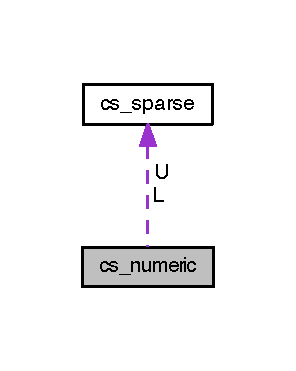
\includegraphics[width=142pt]{structcs__numeric__coll__graph}
\end{center}
\end{figure}
\subsubsection*{Public Attributes}
\begin{DoxyCompactItemize}
\item 
\hyperlink{csparse_8h_a44e471a015cf32e012cffef17e81b6db}{cs} $\ast$ \hyperlink{structcs__numeric_a93a8cf26f01d3df51b41acc690f120d7}{L}
\item 
\hyperlink{csparse_8h_a44e471a015cf32e012cffef17e81b6db}{cs} $\ast$ \hyperlink{structcs__numeric_a1e07204edb10064ca1e471289fced1cb}{U}
\item 
int $\ast$ \hyperlink{structcs__numeric_a485727ef230d7e61b735fad674135d78}{Pinv}
\item 
double $\ast$ \hyperlink{structcs__numeric_ad81bc354670c58c7e715293e98316152}{B}
\end{DoxyCompactItemize}


\subsubsection{Detailed Description}


Definition at line 59 of file csparse.\-h.



\subsubsection{Member Data Documentation}
\hypertarget{structcs__numeric_a93a8cf26f01d3df51b41acc690f120d7}{\index{cs\-\_\-numeric@{cs\-\_\-numeric}!L@{L}}
\index{L@{L}!cs_numeric@{cs\-\_\-numeric}}
\paragraph[{L}]{\setlength{\rightskip}{0pt plus 5cm}{\bf cs}$\ast$ cs\-\_\-numeric\-::\-L}}\label{structcs__numeric_a93a8cf26f01d3df51b41acc690f120d7}


Definition at line 61 of file csparse.\-h.



Referenced by cs\-\_\-chol(), cs\-\_\-cholsol(), cs\-\_\-lu(), cs\-\_\-lusol(), cs\-\_\-nfree(), cs\-\_\-qr(), and cs\-\_\-qrsol().

\hypertarget{structcs__numeric_a1e07204edb10064ca1e471289fced1cb}{\index{cs\-\_\-numeric@{cs\-\_\-numeric}!U@{U}}
\index{U@{U}!cs_numeric@{cs\-\_\-numeric}}
\paragraph[{U}]{\setlength{\rightskip}{0pt plus 5cm}{\bf cs}$\ast$ cs\-\_\-numeric\-::\-U}}\label{structcs__numeric_a1e07204edb10064ca1e471289fced1cb}


Definition at line 62 of file csparse.\-h.



Referenced by cs\-\_\-lu(), cs\-\_\-lusol(), cs\-\_\-nfree(), cs\-\_\-qr(), and cs\-\_\-qrsol().

\hypertarget{structcs__numeric_a485727ef230d7e61b735fad674135d78}{\index{cs\-\_\-numeric@{cs\-\_\-numeric}!Pinv@{Pinv}}
\index{Pinv@{Pinv}!cs_numeric@{cs\-\_\-numeric}}
\paragraph[{Pinv}]{\setlength{\rightskip}{0pt plus 5cm}int$\ast$ cs\-\_\-numeric\-::\-Pinv}}\label{structcs__numeric_a485727ef230d7e61b735fad674135d78}


Definition at line 63 of file csparse.\-h.



Referenced by cs\-\_\-lu(), cs\-\_\-lusol(), and cs\-\_\-nfree().

\hypertarget{structcs__numeric_ad81bc354670c58c7e715293e98316152}{\index{cs\-\_\-numeric@{cs\-\_\-numeric}!B@{B}}
\index{B@{B}!cs_numeric@{cs\-\_\-numeric}}
\paragraph[{B}]{\setlength{\rightskip}{0pt plus 5cm}double$\ast$ cs\-\_\-numeric\-::\-B}}\label{structcs__numeric_ad81bc354670c58c7e715293e98316152}


Definition at line 64 of file csparse.\-h.



Referenced by cs\-\_\-nfree(), cs\-\_\-qr(), and cs\-\_\-qrsol().


\hypertarget{structcs__sparse}{\subsection{cs\-\_\-sparse Struct Reference}
\label{structcs__sparse}\index{cs\-\_\-sparse@{cs\-\_\-sparse}}
}


{\ttfamily \#include $<$csparse.\-h$>$}

\subsubsection*{Public Attributes}
\begin{DoxyCompactItemize}
\item 
int \hyperlink{structcs__sparse_aab49fc365ddf6273376a96d3a6aa751f}{nzmax}
\item 
int \hyperlink{structcs__sparse_a8aeba3ffed4d599a4906e78329d3448b}{m}
\item 
int \hyperlink{structcs__sparse_a86c18870dc1551c71f8ea551efe68625}{n}
\item 
int $\ast$ \hyperlink{structcs__sparse_a263a2347e8dcf1a7a20ee66730297b85}{p}
\item 
int $\ast$ \hyperlink{structcs__sparse_aeb6831b93f8a901b4a5d520c46990f44}{i}
\item 
double $\ast$ \hyperlink{structcs__sparse_a0d6d06e4893a7d4d86e94ce49358d9c1}{x}
\item 
int \hyperlink{structcs__sparse_a707363d7869d3fc4126027c1c9c7cf7c}{nz}
\end{DoxyCompactItemize}


\subsubsection{Detailed Description}


Definition at line 14 of file csparse.\-h.



\subsubsection{Member Data Documentation}
\hypertarget{structcs__sparse_aab49fc365ddf6273376a96d3a6aa751f}{\index{cs\-\_\-sparse@{cs\-\_\-sparse}!nzmax@{nzmax}}
\index{nzmax@{nzmax}!cs_sparse@{cs\-\_\-sparse}}
\paragraph[{nzmax}]{\setlength{\rightskip}{0pt plus 5cm}int cs\-\_\-sparse\-::nzmax}}\label{structcs__sparse_aab49fc365ddf6273376a96d3a6aa751f}


Definition at line 16 of file csparse.\-h.



Referenced by cs\-\_\-amd(), cs\-\_\-entry(), cs\-\_\-lu(), cs\-\_\-print(), cs\-\_\-spalloc(), and cs\-\_\-sprealloc().

\hypertarget{structcs__sparse_a8aeba3ffed4d599a4906e78329d3448b}{\index{cs\-\_\-sparse@{cs\-\_\-sparse}!m@{m}}
\index{m@{m}!cs_sparse@{cs\-\_\-sparse}}
\paragraph[{m}]{\setlength{\rightskip}{0pt plus 5cm}int cs\-\_\-sparse\-::m}}\label{structcs__sparse_a8aeba3ffed4d599a4906e78329d3448b}


Definition at line 17 of file csparse.\-h.



Referenced by cs\-\_\-add(), cs\-\_\-amd(), cs\-\_\-counts(), cs\-\_\-dmperm(), cs\-\_\-dupl(), cs\-\_\-entry(), cs\-\_\-etree(), cs\-\_\-maxtrans(), cs\-\_\-multiply(), cs\-\_\-permute(), cs\-\_\-print(), cs\-\_\-qr(), cs\-\_\-qrsol(), cs\-\_\-spalloc(), cs\-\_\-transpose(), cs\-\_\-triplet(), and cs\-\_\-vcount().

\hypertarget{structcs__sparse_a86c18870dc1551c71f8ea551efe68625}{\index{cs\-\_\-sparse@{cs\-\_\-sparse}!n@{n}}
\index{n@{n}!cs_sparse@{cs\-\_\-sparse}}
\paragraph[{n}]{\setlength{\rightskip}{0pt plus 5cm}int cs\-\_\-sparse\-::n}}\label{structcs__sparse_a86c18870dc1551c71f8ea551efe68625}


Definition at line 18 of file csparse.\-h.



Referenced by cs\-\_\-add(), cs\-\_\-amd(), cs\-\_\-chol(), cs\-\_\-cholsol(), cs\-\_\-counts(), cs\-\_\-dmperm(), cs\-\_\-dupl(), cs\-\_\-entry(), cs\-\_\-etree(), cs\-\_\-fkeep(), cs\-\_\-gaxpy(), cs\-\_\-lsolve(), cs\-\_\-ltsolve(), cs\-\_\-lu(), cs\-\_\-lusol(), cs\-\_\-maxtrans(), cs\-\_\-multiply(), cs\-\_\-norm(), cs\-\_\-permute(), cs\-\_\-print(), cs\-\_\-qr(), cs\-\_\-qrsol(), cs\-\_\-reach(), cs\-\_\-scc(), cs\-\_\-schol(), cs\-\_\-spalloc(), cs\-\_\-splsolve(), cs\-\_\-sprealloc(), cs\-\_\-sqr(), cs\-\_\-symperm(), cs\-\_\-transpose(), cs\-\_\-triplet(), cs\-\_\-updown(), cs\-\_\-usolve(), cs\-\_\-utsolve(), and cs\-\_\-vcount().

\hypertarget{structcs__sparse_a263a2347e8dcf1a7a20ee66730297b85}{\index{cs\-\_\-sparse@{cs\-\_\-sparse}!p@{p}}
\index{p@{p}!cs_sparse@{cs\-\_\-sparse}}
\paragraph[{p}]{\setlength{\rightskip}{0pt plus 5cm}int$\ast$ cs\-\_\-sparse\-::p}}\label{structcs__sparse_a263a2347e8dcf1a7a20ee66730297b85}


Definition at line 19 of file csparse.\-h.



Referenced by cs\-\_\-add(), cs\-\_\-amd(), cs\-\_\-augment(), cs\-\_\-bfs(), cs\-\_\-chol(), cs\-\_\-counts(), cs\-\_\-dfs(), cs\-\_\-dmperm(), cs\-\_\-dupl(), cs\-\_\-entry(), cs\-\_\-ereach(), cs\-\_\-etree(), cs\-\_\-fkeep(), cs\-\_\-gaxpy(), cs\-\_\-happly(), cs\-\_\-lsolve(), cs\-\_\-ltsolve(), cs\-\_\-lu(), cs\-\_\-maxtrans(), cs\-\_\-multiply(), cs\-\_\-norm(), cs\-\_\-permute(), cs\-\_\-print(), cs\-\_\-qr(), cs\-\_\-reach(), cs\-\_\-scatter(), cs\-\_\-scc(), cs\-\_\-spalloc(), cs\-\_\-spfree(), cs\-\_\-splsolve(), cs\-\_\-sprealloc(), cs\-\_\-sqr(), cs\-\_\-symperm(), cs\-\_\-transpose(), cs\-\_\-triplet(), cs\-\_\-updown(), cs\-\_\-usolve(), cs\-\_\-utsolve(), and cs\-\_\-vcount().

\hypertarget{structcs__sparse_aeb6831b93f8a901b4a5d520c46990f44}{\index{cs\-\_\-sparse@{cs\-\_\-sparse}!i@{i}}
\index{i@{i}!cs_sparse@{cs\-\_\-sparse}}
\paragraph[{i}]{\setlength{\rightskip}{0pt plus 5cm}int$\ast$ cs\-\_\-sparse\-::i}}\label{structcs__sparse_aeb6831b93f8a901b4a5d520c46990f44}


Definition at line 20 of file csparse.\-h.



Referenced by cs\-\_\-amd(), cs\-\_\-augment(), cs\-\_\-bfs(), cs\-\_\-chol(), cs\-\_\-counts(), cs\-\_\-dfs(), cs\-\_\-dmperm(), cs\-\_\-dupl(), cs\-\_\-entry(), cs\-\_\-ereach(), cs\-\_\-etree(), cs\-\_\-fkeep(), cs\-\_\-gaxpy(), cs\-\_\-happly(), cs\-\_\-lsolve(), cs\-\_\-ltsolve(), cs\-\_\-lu(), cs\-\_\-maxtrans(), cs\-\_\-multiply(), cs\-\_\-permute(), cs\-\_\-print(), cs\-\_\-qr(), cs\-\_\-reach(), cs\-\_\-scatter(), cs\-\_\-spalloc(), cs\-\_\-spfree(), cs\-\_\-splsolve(), cs\-\_\-sprealloc(), cs\-\_\-symperm(), cs\-\_\-transpose(), cs\-\_\-triplet(), cs\-\_\-updown(), cs\-\_\-usolve(), cs\-\_\-utsolve(), and cs\-\_\-vcount().

\hypertarget{structcs__sparse_a0d6d06e4893a7d4d86e94ce49358d9c1}{\index{cs\-\_\-sparse@{cs\-\_\-sparse}!x@{x}}
\index{x@{x}!cs_sparse@{cs\-\_\-sparse}}
\paragraph[{x}]{\setlength{\rightskip}{0pt plus 5cm}double$\ast$ cs\-\_\-sparse\-::x}}\label{structcs__sparse_a0d6d06e4893a7d4d86e94ce49358d9c1}


Definition at line 21 of file csparse.\-h.



Referenced by cs\-\_\-add(), cs\-\_\-chol(), cs\-\_\-dupl(), cs\-\_\-entry(), cs\-\_\-ereach(), cs\-\_\-fkeep(), cs\-\_\-gaxpy(), cs\-\_\-happly(), cs\-\_\-lsolve(), cs\-\_\-ltsolve(), cs\-\_\-lu(), cs\-\_\-multiply(), cs\-\_\-norm(), cs\-\_\-permute(), cs\-\_\-print(), cs\-\_\-qr(), cs\-\_\-scatter(), cs\-\_\-spalloc(), cs\-\_\-spfree(), cs\-\_\-splsolve(), cs\-\_\-sprealloc(), cs\-\_\-symperm(), cs\-\_\-transpose(), cs\-\_\-triplet(), cs\-\_\-updown(), cs\-\_\-usolve(), and cs\-\_\-utsolve().

\hypertarget{structcs__sparse_a707363d7869d3fc4126027c1c9c7cf7c}{\index{cs\-\_\-sparse@{cs\-\_\-sparse}!nz@{nz}}
\index{nz@{nz}!cs_sparse@{cs\-\_\-sparse}}
\paragraph[{nz}]{\setlength{\rightskip}{0pt plus 5cm}int cs\-\_\-sparse\-::nz}}\label{structcs__sparse_a707363d7869d3fc4126027c1c9c7cf7c}


Definition at line 22 of file csparse.\-h.



Referenced by cs\-\_\-entry(), cs\-\_\-print(), cs\-\_\-spalloc(), cs\-\_\-sprealloc(), and cs\-\_\-triplet().


\hypertarget{structcs__symbolic}{\subsection{cs\-\_\-symbolic Struct Reference}
\label{structcs__symbolic}\index{cs\-\_\-symbolic@{cs\-\_\-symbolic}}
}


{\ttfamily \#include $<$csparse.\-h$>$}

\subsubsection*{Public Attributes}
\begin{DoxyCompactItemize}
\item 
int $\ast$ \hyperlink{structcs__symbolic_a095ba468af8cb63c4cecf46a1adb45ac}{Pinv}
\item 
int $\ast$ \hyperlink{structcs__symbolic_afcefa00ab98cf91d2258dc5a63f7dd6d}{Q}
\item 
int $\ast$ \hyperlink{structcs__symbolic_aefc6fc6ae59f5c51b225c93a549b6838}{parent}
\item 
int $\ast$ \hyperlink{structcs__symbolic_a85eed6fd134282ada142ebaae0fe2403}{cp}
\item 
int \hyperlink{structcs__symbolic_a6e76dde6232a98e3b5d96d942c08b12e}{m2}
\item 
int \hyperlink{structcs__symbolic_acfb8969ebae172c2efcc82e1b98ef826}{lnz}
\item 
int \hyperlink{structcs__symbolic_ad20740ef6e60d2a90e12860c0bf6aab7}{unz}
\end{DoxyCompactItemize}


\subsubsection{Detailed Description}


Definition at line 48 of file csparse.\-h.



\subsubsection{Member Data Documentation}
\hypertarget{structcs__symbolic_a095ba468af8cb63c4cecf46a1adb45ac}{\index{cs\-\_\-symbolic@{cs\-\_\-symbolic}!Pinv@{Pinv}}
\index{Pinv@{Pinv}!cs_symbolic@{cs\-\_\-symbolic}}
\paragraph[{Pinv}]{\setlength{\rightskip}{0pt plus 5cm}int$\ast$ cs\-\_\-symbolic\-::\-Pinv}}\label{structcs__symbolic_a095ba468af8cb63c4cecf46a1adb45ac}


Definition at line 50 of file csparse.\-h.



Referenced by cs\-\_\-chol(), cs\-\_\-cholsol(), cs\-\_\-qr(), cs\-\_\-qrsol(), cs\-\_\-schol(), cs\-\_\-sfree(), and cs\-\_\-sqr().

\hypertarget{structcs__symbolic_afcefa00ab98cf91d2258dc5a63f7dd6d}{\index{cs\-\_\-symbolic@{cs\-\_\-symbolic}!Q@{Q}}
\index{Q@{Q}!cs_symbolic@{cs\-\_\-symbolic}}
\paragraph[{Q}]{\setlength{\rightskip}{0pt plus 5cm}int$\ast$ cs\-\_\-symbolic\-::\-Q}}\label{structcs__symbolic_afcefa00ab98cf91d2258dc5a63f7dd6d}


Definition at line 51 of file csparse.\-h.



Referenced by cs\-\_\-lu(), cs\-\_\-lusol(), cs\-\_\-qr(), cs\-\_\-qrsol(), cs\-\_\-sfree(), and cs\-\_\-sqr().

\hypertarget{structcs__symbolic_aefc6fc6ae59f5c51b225c93a549b6838}{\index{cs\-\_\-symbolic@{cs\-\_\-symbolic}!parent@{parent}}
\index{parent@{parent}!cs_symbolic@{cs\-\_\-symbolic}}
\paragraph[{parent}]{\setlength{\rightskip}{0pt plus 5cm}int$\ast$ cs\-\_\-symbolic\-::parent}}\label{structcs__symbolic_aefc6fc6ae59f5c51b225c93a549b6838}


Definition at line 52 of file csparse.\-h.



Referenced by cs\-\_\-chol(), cs\-\_\-qr(), cs\-\_\-schol(), cs\-\_\-sfree(), and cs\-\_\-sqr().

\hypertarget{structcs__symbolic_a85eed6fd134282ada142ebaae0fe2403}{\index{cs\-\_\-symbolic@{cs\-\_\-symbolic}!cp@{cp}}
\index{cp@{cp}!cs_symbolic@{cs\-\_\-symbolic}}
\paragraph[{cp}]{\setlength{\rightskip}{0pt plus 5cm}int$\ast$ cs\-\_\-symbolic\-::cp}}\label{structcs__symbolic_a85eed6fd134282ada142ebaae0fe2403}


Definition at line 53 of file csparse.\-h.



Referenced by cs\-\_\-chol(), cs\-\_\-schol(), cs\-\_\-sfree(), and cs\-\_\-sqr().

\hypertarget{structcs__symbolic_a6e76dde6232a98e3b5d96d942c08b12e}{\index{cs\-\_\-symbolic@{cs\-\_\-symbolic}!m2@{m2}}
\index{m2@{m2}!cs_symbolic@{cs\-\_\-symbolic}}
\paragraph[{m2}]{\setlength{\rightskip}{0pt plus 5cm}int cs\-\_\-symbolic\-::m2}}\label{structcs__symbolic_a6e76dde6232a98e3b5d96d942c08b12e}


Definition at line 54 of file csparse.\-h.



Referenced by cs\-\_\-qr(), cs\-\_\-qrsol(), and cs\-\_\-sqr().

\hypertarget{structcs__symbolic_acfb8969ebae172c2efcc82e1b98ef826}{\index{cs\-\_\-symbolic@{cs\-\_\-symbolic}!lnz@{lnz}}
\index{lnz@{lnz}!cs_symbolic@{cs\-\_\-symbolic}}
\paragraph[{lnz}]{\setlength{\rightskip}{0pt plus 5cm}int cs\-\_\-symbolic\-::lnz}}\label{structcs__symbolic_acfb8969ebae172c2efcc82e1b98ef826}


Definition at line 55 of file csparse.\-h.



Referenced by cs\-\_\-lu(), cs\-\_\-qr(), cs\-\_\-schol(), and cs\-\_\-sqr().

\hypertarget{structcs__symbolic_ad20740ef6e60d2a90e12860c0bf6aab7}{\index{cs\-\_\-symbolic@{cs\-\_\-symbolic}!unz@{unz}}
\index{unz@{unz}!cs_symbolic@{cs\-\_\-symbolic}}
\paragraph[{unz}]{\setlength{\rightskip}{0pt plus 5cm}int cs\-\_\-symbolic\-::unz}}\label{structcs__symbolic_ad20740ef6e60d2a90e12860c0bf6aab7}


Definition at line 56 of file csparse.\-h.



Referenced by cs\-\_\-lu(), cs\-\_\-qr(), cs\-\_\-schol(), and cs\-\_\-sqr().


\hypertarget{structfclib__global}{\subsection{fclib\-\_\-global Struct Reference}
\label{structfclib__global}\index{fclib\-\_\-global@{fclib\-\_\-global}}
}


The global frictional contact problem defined by.  




{\ttfamily \#include $<$fclib.\-h$>$}



Collaboration diagram for fclib\-\_\-global\-:\nopagebreak
\begin{figure}[H]
\begin{center}
\leavevmode
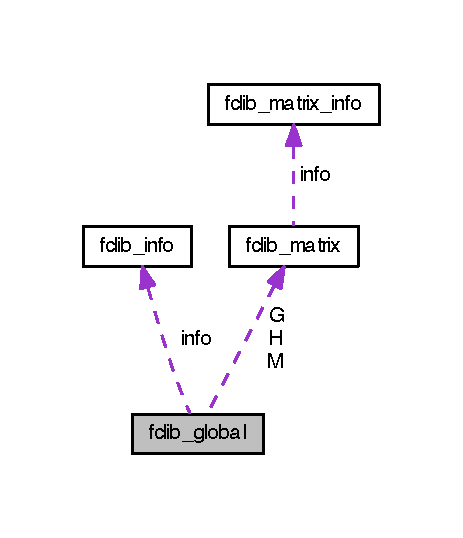
\includegraphics[width=222pt]{structfclib__global__coll__graph}
\end{center}
\end{figure}
\subsubsection*{Public Attributes}
\begin{DoxyCompactItemize}
\item 
struct \hyperlink{structfclib__matrix}{fclib\-\_\-matrix} $\ast$ \hyperlink{structfclib__global_a82538cefd07d0f1f6c1e7baebe768fc6}{M}
\begin{DoxyCompactList}\small\item\em the matrix M (see mathematical description below) \end{DoxyCompactList}\item 
struct \hyperlink{structfclib__matrix}{fclib\-\_\-matrix} $\ast$ \hyperlink{structfclib__global_ac87d5553d144625b9006e2e8b0c89b3c}{H}
\begin{DoxyCompactList}\small\item\em the matrix M (see mathematical description below) \end{DoxyCompactList}\item 
struct \hyperlink{structfclib__matrix}{fclib\-\_\-matrix} $\ast$ \hyperlink{structfclib__global_a897c09aca4a010076ed9ddb3f7527a79}{G}
\begin{DoxyCompactList}\small\item\em the matrix M (see mathematical description below) \end{DoxyCompactList}\item 
double $\ast$ \hyperlink{structfclib__global_a99fd8c775c35a6a0e233df1f8cae181a}{mu}
\begin{DoxyCompactList}\small\item\em the vector $\mu$ of coefficient of friction (see mathematical description below) \end{DoxyCompactList}\item 
double $\ast$ \hyperlink{structfclib__global_a6d5d0d1f9169b886eb3d3aca0632e8a9}{f}
\begin{DoxyCompactList}\small\item\em the vector f (see mathematical description below) \end{DoxyCompactList}\item 
double $\ast$ \hyperlink{structfclib__global_a1badf3df92b120566a2ee3c42194972f}{b}
\begin{DoxyCompactList}\small\item\em the vector b (see mathematical description below) \end{DoxyCompactList}\item 
double $\ast$ \hyperlink{structfclib__global_a8b175716b6c1f84509cf44b36a76e7ca}{w}
\begin{DoxyCompactList}\small\item\em the vector w (see mathematical description below) \end{DoxyCompactList}\item 
int \hyperlink{structfclib__global_a86dac5928d2c652f15ac688df14989a0}{spacedim}
\begin{DoxyCompactList}\small\item\em the dimension , 2 or 3, of the local space at contact (2d or 3d friction contact laws) \end{DoxyCompactList}\item 
struct \hyperlink{structfclib__info}{fclib\-\_\-info} $\ast$ \hyperlink{structfclib__global_aa6b4e80afc92dd1a9b260ff3a096b352}{info}
\begin{DoxyCompactList}\small\item\em info on the problem \end{DoxyCompactList}\end{DoxyCompactItemize}


\subsubsection{Detailed Description}
The global frictional contact problem defined by. 

Given 
\begin{DoxyItemize}
\item a symmetric positive definite matrix ${M} \in {\mathrm{I\!R}}^{n \times n}$ 
\item a vector $ {f} \in {\mathrm{I\!R}}^n$, 
\item a matrix ${H} \in {\mathrm{I\!R}}^{n \times m}$ 
\item a matrix ${G} \in {\mathrm{I\!R}}^{n \times p}$ 
\item a vector $w \in {\mathrm{I\!R}}^{m}$, 
\item a vector $b \in {\mathrm{I\!R}}^{p}$, 
\item a vector of coefficients of friction $\mu \in {\mathrm{I\!R}}^{n_c}$ 
\end{DoxyItemize}the Global Mixed 3\-D\-F\-C problem is to find four vectors $ {v} \in {\mathrm{I\!R}}^n$, $u\in{\mathrm{I\!R}}^m$, $r\in {\mathrm{I\!R}}^m$ and $\lambda \in {\mathrm{I\!R}}^p$ denoted by $\mathrm{GM3DFC}(M,H,G,w,b,\mu)$ such that \begin{eqnarray*} \begin{cases} M v = {H} {r} + G\lambda + {f} \\ \ \ G^T v +b =0 \\ \ \ \hat u = H^T v + w +\left[ \left[\begin{array}{c} \mu \|u^\alpha_T\|\ \ 0 \ \ 0 \end{array}\right]^T, \alpha = 1 \ldots n_c \right]^T \\ \ \ C^\star_{\mu} \ni {\hat u} \perp r \in C_{\mu} \end{cases} \end{eqnarray*} where the Coulomb friction cone for a contact $\alpha$ is defined by \begin{eqnarray*} \label{eq:CCC} C_{\mu^\alpha}^{\alpha} = \{r^\alpha, \|r^\alpha_T \| \leq \mu^\alpha |r^\alpha_N| \} *\end{eqnarray*} and the set $C^{\alpha,\star}_{\mu^\alpha}$ is its dual. 

Definition at line 174 of file fclib.\-h.



\subsubsection{Member Data Documentation}
\hypertarget{structfclib__global_a82538cefd07d0f1f6c1e7baebe768fc6}{\index{fclib\-\_\-global@{fclib\-\_\-global}!M@{M}}
\index{M@{M}!fclib_global@{fclib\-\_\-global}}
\paragraph[{M}]{\setlength{\rightskip}{0pt plus 5cm}struct {\bf fclib\-\_\-matrix}$\ast$ fclib\-\_\-global\-::\-M}}\label{structfclib__global_a82538cefd07d0f1f6c1e7baebe768fc6}


the matrix M (see mathematical description below) 



Definition at line 177 of file fclib.\-h.



Referenced by compare\-\_\-global\-\_\-problems(), fclib\-\_\-delete\-\_\-global(), fclib\-\_\-read\-\_\-global(), fclib\-\_\-write\-\_\-global(), main(), random\-\_\-global\-\_\-problem(), random\-\_\-global\-\_\-solutions(), read\-\_\-global\-\_\-vectors(), and write\-\_\-global\-\_\-vectors().

\hypertarget{structfclib__global_ac87d5553d144625b9006e2e8b0c89b3c}{\index{fclib\-\_\-global@{fclib\-\_\-global}!H@{H}}
\index{H@{H}!fclib_global@{fclib\-\_\-global}}
\paragraph[{H}]{\setlength{\rightskip}{0pt plus 5cm}struct {\bf fclib\-\_\-matrix}$\ast$ fclib\-\_\-global\-::\-H}}\label{structfclib__global_ac87d5553d144625b9006e2e8b0c89b3c}


the matrix M (see mathematical description below) 



Definition at line 179 of file fclib.\-h.



Referenced by compare\-\_\-global\-\_\-problems(), fclib\-\_\-delete\-\_\-global(), fclib\-\_\-read\-\_\-global(), fclib\-\_\-write\-\_\-global(), main(), random\-\_\-global\-\_\-problem(), random\-\_\-global\-\_\-solutions(), read\-\_\-global\-\_\-vectors(), and write\-\_\-global\-\_\-vectors().

\hypertarget{structfclib__global_a897c09aca4a010076ed9ddb3f7527a79}{\index{fclib\-\_\-global@{fclib\-\_\-global}!G@{G}}
\index{G@{G}!fclib_global@{fclib\-\_\-global}}
\paragraph[{G}]{\setlength{\rightskip}{0pt plus 5cm}struct {\bf fclib\-\_\-matrix}$\ast$ fclib\-\_\-global\-::\-G}}\label{structfclib__global_a897c09aca4a010076ed9ddb3f7527a79}


the matrix M (see mathematical description below) 



Definition at line 181 of file fclib.\-h.



Referenced by compare\-\_\-global\-\_\-problems(), fclib\-\_\-delete\-\_\-global(), fclib\-\_\-read\-\_\-global(), fclib\-\_\-write\-\_\-global(), main(), random\-\_\-global\-\_\-problem(), random\-\_\-global\-\_\-solutions(), read\-\_\-global\-\_\-vectors(), and write\-\_\-global\-\_\-vectors().

\hypertarget{structfclib__global_a99fd8c775c35a6a0e233df1f8cae181a}{\index{fclib\-\_\-global@{fclib\-\_\-global}!mu@{mu}}
\index{mu@{mu}!fclib_global@{fclib\-\_\-global}}
\paragraph[{mu}]{\setlength{\rightskip}{0pt plus 5cm}double$\ast$ fclib\-\_\-global\-::mu}}\label{structfclib__global_a99fd8c775c35a6a0e233df1f8cae181a}


the vector $\mu$ of coefficient of friction (see mathematical description below) 



Definition at line 183 of file fclib.\-h.



Referenced by compare\-\_\-global\-\_\-problems(), fclib\-\_\-delete\-\_\-global(), random\-\_\-global\-\_\-problem(), read\-\_\-global\-\_\-vectors(), and write\-\_\-global\-\_\-vectors().

\hypertarget{structfclib__global_a6d5d0d1f9169b886eb3d3aca0632e8a9}{\index{fclib\-\_\-global@{fclib\-\_\-global}!f@{f}}
\index{f@{f}!fclib_global@{fclib\-\_\-global}}
\paragraph[{f}]{\setlength{\rightskip}{0pt plus 5cm}double$\ast$ fclib\-\_\-global\-::f}}\label{structfclib__global_a6d5d0d1f9169b886eb3d3aca0632e8a9}


the vector f (see mathematical description below) 



Definition at line 185 of file fclib.\-h.



Referenced by compare\-\_\-global\-\_\-problems(), fclib\-\_\-delete\-\_\-global(), random\-\_\-global\-\_\-problem(), read\-\_\-global\-\_\-vectors(), and write\-\_\-global\-\_\-vectors().

\hypertarget{structfclib__global_a1badf3df92b120566a2ee3c42194972f}{\index{fclib\-\_\-global@{fclib\-\_\-global}!b@{b}}
\index{b@{b}!fclib_global@{fclib\-\_\-global}}
\paragraph[{b}]{\setlength{\rightskip}{0pt plus 5cm}double$\ast$ fclib\-\_\-global\-::b}}\label{structfclib__global_a1badf3df92b120566a2ee3c42194972f}


the vector b (see mathematical description below) 



Definition at line 187 of file fclib.\-h.



Referenced by compare\-\_\-global\-\_\-problems(), fclib\-\_\-delete\-\_\-global(), random\-\_\-global\-\_\-problem(), read\-\_\-global\-\_\-vectors(), and write\-\_\-global\-\_\-vectors().

\hypertarget{structfclib__global_a8b175716b6c1f84509cf44b36a76e7ca}{\index{fclib\-\_\-global@{fclib\-\_\-global}!w@{w}}
\index{w@{w}!fclib_global@{fclib\-\_\-global}}
\paragraph[{w}]{\setlength{\rightskip}{0pt plus 5cm}double$\ast$ fclib\-\_\-global\-::w}}\label{structfclib__global_a8b175716b6c1f84509cf44b36a76e7ca}


the vector w (see mathematical description below) 



Definition at line 189 of file fclib.\-h.



Referenced by compare\-\_\-global\-\_\-problems(), fclib\-\_\-delete\-\_\-global(), random\-\_\-global\-\_\-problem(), read\-\_\-global\-\_\-vectors(), and write\-\_\-global\-\_\-vectors().

\hypertarget{structfclib__global_a86dac5928d2c652f15ac688df14989a0}{\index{fclib\-\_\-global@{fclib\-\_\-global}!spacedim@{spacedim}}
\index{spacedim@{spacedim}!fclib_global@{fclib\-\_\-global}}
\paragraph[{spacedim}]{\setlength{\rightskip}{0pt plus 5cm}int fclib\-\_\-global\-::spacedim}}\label{structfclib__global_a86dac5928d2c652f15ac688df14989a0}


the dimension , 2 or 3, of the local space at contact (2d or 3d friction contact laws) 



Definition at line 191 of file fclib.\-h.



Referenced by compare\-\_\-global\-\_\-problems(), fclib\-\_\-read\-\_\-global(), fclib\-\_\-write\-\_\-global(), random\-\_\-global\-\_\-problem(), read\-\_\-global\-\_\-vectors(), and write\-\_\-global\-\_\-vectors().

\hypertarget{structfclib__global_aa6b4e80afc92dd1a9b260ff3a096b352}{\index{fclib\-\_\-global@{fclib\-\_\-global}!info@{info}}
\index{info@{info}!fclib_global@{fclib\-\_\-global}}
\paragraph[{info}]{\setlength{\rightskip}{0pt plus 5cm}struct {\bf fclib\-\_\-info}$\ast$ fclib\-\_\-global\-::info}}\label{structfclib__global_aa6b4e80afc92dd1a9b260ff3a096b352}


info on the problem 



Definition at line 193 of file fclib.\-h.



Referenced by compare\-\_\-global\-\_\-problems(), fclib\-\_\-delete\-\_\-global(), fclib\-\_\-read\-\_\-global(), fclib\-\_\-write\-\_\-global(), and random\-\_\-global\-\_\-problem().


\hypertarget{structfclib__info}{\subsection{fclib\-\_\-info Struct Reference}
\label{structfclib__info}\index{fclib\-\_\-info@{fclib\-\_\-info}}
}


This structure allows the user to enter a problem information as a title, a short description and known mathematical properties of the problem.  




{\ttfamily \#include $<$fclib.\-h$>$}

\subsubsection*{Public Attributes}
\begin{DoxyCompactItemize}
\item 
char $\ast$ \hyperlink{structfclib__info_a4ea1b298e3aa7228a5f2a55f711f41d2}{title}
\begin{DoxyCompactList}\small\item\em title of the problem \end{DoxyCompactList}\item 
char $\ast$ \hyperlink{structfclib__info_a0c1680fee67eaf7b20c436a775d4f35d}{description}
\begin{DoxyCompactList}\small\item\em short decription of the problem \end{DoxyCompactList}\item 
char $\ast$ \hyperlink{structfclib__info_ad6dadb3af34a719e5ec3cab2d499c7f2}{math\-\_\-info}
\begin{DoxyCompactList}\small\item\em known properties of the problem (existence, uniqueness, ...) \end{DoxyCompactList}\end{DoxyCompactItemize}


\subsubsection{Detailed Description}
This structure allows the user to enter a problem information as a title, a short description and known mathematical properties of the problem. 

Definition at line 91 of file fclib.\-h.



\subsubsection{Member Data Documentation}
\hypertarget{structfclib__info_a4ea1b298e3aa7228a5f2a55f711f41d2}{\index{fclib\-\_\-info@{fclib\-\_\-info}!title@{title}}
\index{title@{title}!fclib_info@{fclib\-\_\-info}}
\paragraph[{title}]{\setlength{\rightskip}{0pt plus 5cm}char$\ast$ fclib\-\_\-info\-::title}}\label{structfclib__info_a4ea1b298e3aa7228a5f2a55f711f41d2}


title of the problem 



Definition at line 94 of file fclib.\-h.



Referenced by compare\-\_\-infos(), delete\-\_\-info(), problem\-\_\-info(), read\-\_\-problem\-\_\-info(), and write\-\_\-problem\-\_\-info().

\hypertarget{structfclib__info_a0c1680fee67eaf7b20c436a775d4f35d}{\index{fclib\-\_\-info@{fclib\-\_\-info}!description@{description}}
\index{description@{description}!fclib_info@{fclib\-\_\-info}}
\paragraph[{description}]{\setlength{\rightskip}{0pt plus 5cm}char$\ast$ fclib\-\_\-info\-::description}}\label{structfclib__info_a0c1680fee67eaf7b20c436a775d4f35d}


short decription of the problem 



Definition at line 96 of file fclib.\-h.



Referenced by compare\-\_\-infos(), delete\-\_\-info(), problem\-\_\-info(), read\-\_\-problem\-\_\-info(), and write\-\_\-problem\-\_\-info().

\hypertarget{structfclib__info_ad6dadb3af34a719e5ec3cab2d499c7f2}{\index{fclib\-\_\-info@{fclib\-\_\-info}!math\-\_\-info@{math\-\_\-info}}
\index{math\-\_\-info@{math\-\_\-info}!fclib_info@{fclib\-\_\-info}}
\paragraph[{math\-\_\-info}]{\setlength{\rightskip}{0pt plus 5cm}char$\ast$ fclib\-\_\-info\-::math\-\_\-info}}\label{structfclib__info_ad6dadb3af34a719e5ec3cab2d499c7f2}


known properties of the problem (existence, uniqueness, ...) 



Definition at line 98 of file fclib.\-h.



Referenced by compare\-\_\-infos(), delete\-\_\-info(), problem\-\_\-info(), read\-\_\-problem\-\_\-info(), and write\-\_\-problem\-\_\-info().


\hypertarget{structfclib__local}{\subsection{fclib\-\_\-local Struct Reference}
\label{structfclib__local}\index{fclib\-\_\-local@{fclib\-\_\-local}}
}


The local frictional contact problem defined by.  




{\ttfamily \#include $<$fclib.\-h$>$}



Collaboration diagram for fclib\-\_\-local\-:\nopagebreak
\begin{figure}[H]
\begin{center}
\leavevmode
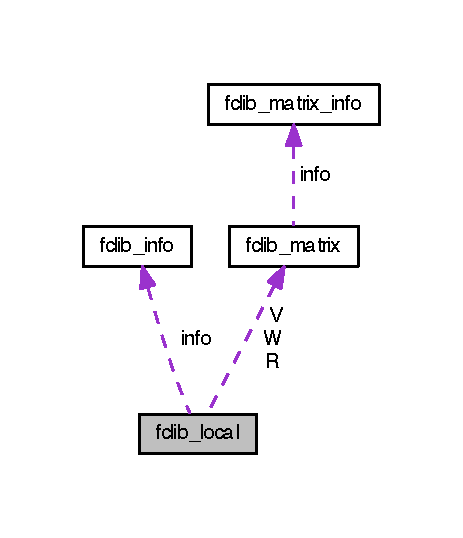
\includegraphics[width=222pt]{structfclib__local__coll__graph}
\end{center}
\end{figure}
\subsubsection*{Public Attributes}
\begin{DoxyCompactItemize}
\item 
struct \hyperlink{structfclib__matrix}{fclib\-\_\-matrix} $\ast$ \hyperlink{structfclib__local_a981b5abb9acf3f99dffe9a05602ad864}{W}
\begin{DoxyCompactList}\small\item\em the matrix W (see mathematical description below) \end{DoxyCompactList}\item 
struct \hyperlink{structfclib__matrix}{fclib\-\_\-matrix} $\ast$ \hyperlink{structfclib__local_a516663ee92260f82283b4933f7e098cf}{V}
\begin{DoxyCompactList}\small\item\em the matrix V (see mathematical description below) \end{DoxyCompactList}\item 
struct \hyperlink{structfclib__matrix}{fclib\-\_\-matrix} $\ast$ \hyperlink{structfclib__local_ae08751b33a0771d54d48aee48f838ced}{R}
\begin{DoxyCompactList}\small\item\em the matrix R (see mathematical description below) \end{DoxyCompactList}\item 
double $\ast$ \hyperlink{structfclib__local_a90d9490cac0bc9b69fd13253882f1557}{mu}
\begin{DoxyCompactList}\small\item\em the vector $\mu$ of coefficient of friction (see mathematical description below) \end{DoxyCompactList}\item 
double $\ast$ \hyperlink{structfclib__local_a9a032092a828a13a7e106cce4ba7ad96}{q}
\begin{DoxyCompactList}\small\item\em the vector q (see mathematical description below) \end{DoxyCompactList}\item 
double $\ast$ \hyperlink{structfclib__local_abb6b3a07d92a86aac1c38e4d847207e3}{s}
\begin{DoxyCompactList}\small\item\em the vector s (see mathematical description below) \end{DoxyCompactList}\item 
int \hyperlink{structfclib__local_accf07018913652e57be3a661b25d8bb7}{spacedim}
\begin{DoxyCompactList}\small\item\em the dimension , 2 or 3, of the local space at contact (2d or 3d friction contact laws) \end{DoxyCompactList}\item 
struct \hyperlink{structfclib__info}{fclib\-\_\-info} $\ast$ \hyperlink{structfclib__local_ababce9da71cdb99e4928a596dde8bc89}{info}
\begin{DoxyCompactList}\small\item\em info on the problem \end{DoxyCompactList}\end{DoxyCompactItemize}


\subsubsection{Detailed Description}
The local frictional contact problem defined by. 

given 
\begin{DoxyItemize}
\item a positive semi--definite matrix ${W} \in {\mathrm{I\!R}}^{m \times m}$ 
\item a matrix ${V} \in {\mathrm{I\!R}}^{m \times p}$ 
\item a matrix ${R} \in {\mathrm{I\!R}}^{p \times p}$ 
\item a vector $q \in {\mathrm{I\!R}}^{m}$, 
\item a vector $s \in {\mathrm{I\!R}}^{p}$, 
\item a vector of coefficients of friction $\mu \in {\mathrm{I\!R}}^{n_c}$ 
\end{DoxyItemize}the Mixed 3\-D\-F\-C problem is to find three vectors $u\in{\mathrm{I\!R}}^m$, $r\in {\mathrm{I\!R}}^m$ and $\lambda \in {\mathrm{I\!R}}^p$ denoted by $\mathrm{M3DFC}(R,V,W,q,s,\mu)$ such that \begin{eqnarray*}\label{eq:lcp1} *\begin{cases} V^T {r} + R \lambda + s = 0 \\ \ \ \hat u = W {r} + V\lambda + q +\left[ \left[\begin{array}{c} \mu^\alpha \|u^\alpha_T\|\ \ 0 \ \ 0 \end{array}\right]^T, \alpha = 1 \ldots n_c \right]^T \\ \ \ C^\star_{\mu} \ni {\hat u} \perp r \in C_{\mu} \end{cases} \end{eqnarray*} where the Coulomb friction cone for a contact $\alpha$ is defined by \begin{eqnarray*} \label{eq:CCC} C_{\mu^\alpha}^{\alpha} = \{r^\alpha, \|r^\alpha_T \| \leq \mu^\alpha |r^\alpha_N| \} \end{eqnarray*} and the set $C^{\alpha,\star}_{\mu^\alpha}$ is its dual. 

Definition at line 228 of file fclib.\-h.



\subsubsection{Member Data Documentation}
\hypertarget{structfclib__local_a981b5abb9acf3f99dffe9a05602ad864}{\index{fclib\-\_\-local@{fclib\-\_\-local}!W@{W}}
\index{W@{W}!fclib_local@{fclib\-\_\-local}}
\paragraph[{W}]{\setlength{\rightskip}{0pt plus 5cm}struct {\bf fclib\-\_\-matrix}$\ast$ fclib\-\_\-local\-::\-W}}\label{structfclib__local_a981b5abb9acf3f99dffe9a05602ad864}


the matrix W (see mathematical description below) 



Definition at line 231 of file fclib.\-h.



Referenced by compare\-\_\-local\-\_\-problems(), fclib\-\_\-delete\-\_\-local(), fclib\-\_\-merit\-\_\-local(), fclib\-\_\-read\-\_\-local(), fclib\-\_\-write\-\_\-local(), main(), random\-\_\-local\-\_\-problem(), random\-\_\-local\-\_\-solutions(), read\-\_\-local\-\_\-vectors(), and write\-\_\-local\-\_\-vectors().

\hypertarget{structfclib__local_a516663ee92260f82283b4933f7e098cf}{\index{fclib\-\_\-local@{fclib\-\_\-local}!V@{V}}
\index{V@{V}!fclib_local@{fclib\-\_\-local}}
\paragraph[{V}]{\setlength{\rightskip}{0pt plus 5cm}struct {\bf fclib\-\_\-matrix}$\ast$ fclib\-\_\-local\-::\-V}}\label{structfclib__local_a516663ee92260f82283b4933f7e098cf}


the matrix V (see mathematical description below) 



Definition at line 233 of file fclib.\-h.



Referenced by compare\-\_\-local\-\_\-problems(), fclib\-\_\-delete\-\_\-local(), fclib\-\_\-merit\-\_\-local(), fclib\-\_\-read\-\_\-local(), fclib\-\_\-write\-\_\-local(), random\-\_\-local\-\_\-problem(), and write\-\_\-local\-\_\-vectors().

\hypertarget{structfclib__local_ae08751b33a0771d54d48aee48f838ced}{\index{fclib\-\_\-local@{fclib\-\_\-local}!R@{R}}
\index{R@{R}!fclib_local@{fclib\-\_\-local}}
\paragraph[{R}]{\setlength{\rightskip}{0pt plus 5cm}struct {\bf fclib\-\_\-matrix}$\ast$ fclib\-\_\-local\-::\-R}}\label{structfclib__local_ae08751b33a0771d54d48aee48f838ced}


the matrix R (see mathematical description below) 



Definition at line 235 of file fclib.\-h.



Referenced by compare\-\_\-local\-\_\-problems(), fclib\-\_\-delete\-\_\-local(), fclib\-\_\-merit\-\_\-local(), fclib\-\_\-read\-\_\-local(), fclib\-\_\-write\-\_\-local(), main(), random\-\_\-local\-\_\-problem(), random\-\_\-local\-\_\-solutions(), read\-\_\-local\-\_\-vectors(), and write\-\_\-local\-\_\-vectors().

\hypertarget{structfclib__local_a90d9490cac0bc9b69fd13253882f1557}{\index{fclib\-\_\-local@{fclib\-\_\-local}!mu@{mu}}
\index{mu@{mu}!fclib_local@{fclib\-\_\-local}}
\paragraph[{mu}]{\setlength{\rightskip}{0pt plus 5cm}double$\ast$ fclib\-\_\-local\-::mu}}\label{structfclib__local_a90d9490cac0bc9b69fd13253882f1557}


the vector $\mu$ of coefficient of friction (see mathematical description below) 



Definition at line 237 of file fclib.\-h.



Referenced by compare\-\_\-local\-\_\-problems(), fclib\-\_\-delete\-\_\-local(), fclib\-\_\-merit\-\_\-local(), random\-\_\-local\-\_\-problem(), read\-\_\-local\-\_\-vectors(), and write\-\_\-local\-\_\-vectors().

\hypertarget{structfclib__local_a9a032092a828a13a7e106cce4ba7ad96}{\index{fclib\-\_\-local@{fclib\-\_\-local}!q@{q}}
\index{q@{q}!fclib_local@{fclib\-\_\-local}}
\paragraph[{q}]{\setlength{\rightskip}{0pt plus 5cm}double$\ast$ fclib\-\_\-local\-::q}}\label{structfclib__local_a9a032092a828a13a7e106cce4ba7ad96}


the vector q (see mathematical description below) 



Definition at line 239 of file fclib.\-h.



Referenced by compare\-\_\-local\-\_\-problems(), fclib\-\_\-delete\-\_\-local(), fclib\-\_\-merit\-\_\-local(), random\-\_\-local\-\_\-problem(), read\-\_\-local\-\_\-vectors(), and write\-\_\-local\-\_\-vectors().

\hypertarget{structfclib__local_abb6b3a07d92a86aac1c38e4d847207e3}{\index{fclib\-\_\-local@{fclib\-\_\-local}!s@{s}}
\index{s@{s}!fclib_local@{fclib\-\_\-local}}
\paragraph[{s}]{\setlength{\rightskip}{0pt plus 5cm}double$\ast$ fclib\-\_\-local\-::s}}\label{structfclib__local_abb6b3a07d92a86aac1c38e4d847207e3}


the vector s (see mathematical description below) 



Definition at line 241 of file fclib.\-h.



Referenced by compare\-\_\-local\-\_\-problems(), fclib\-\_\-delete\-\_\-local(), fclib\-\_\-merit\-\_\-local(), random\-\_\-local\-\_\-problem(), read\-\_\-local\-\_\-vectors(), and write\-\_\-local\-\_\-vectors().

\hypertarget{structfclib__local_accf07018913652e57be3a661b25d8bb7}{\index{fclib\-\_\-local@{fclib\-\_\-local}!spacedim@{spacedim}}
\index{spacedim@{spacedim}!fclib_local@{fclib\-\_\-local}}
\paragraph[{spacedim}]{\setlength{\rightskip}{0pt plus 5cm}int fclib\-\_\-local\-::spacedim}}\label{structfclib__local_accf07018913652e57be3a661b25d8bb7}


the dimension , 2 or 3, of the local space at contact (2d or 3d friction contact laws) 



Definition at line 243 of file fclib.\-h.



Referenced by compare\-\_\-local\-\_\-problems(), fclib\-\_\-merit\-\_\-local(), fclib\-\_\-read\-\_\-local(), fclib\-\_\-write\-\_\-local(), random\-\_\-local\-\_\-problem(), read\-\_\-local\-\_\-vectors(), and write\-\_\-local\-\_\-vectors().

\hypertarget{structfclib__local_ababce9da71cdb99e4928a596dde8bc89}{\index{fclib\-\_\-local@{fclib\-\_\-local}!info@{info}}
\index{info@{info}!fclib_local@{fclib\-\_\-local}}
\paragraph[{info}]{\setlength{\rightskip}{0pt plus 5cm}struct {\bf fclib\-\_\-info}$\ast$ fclib\-\_\-local\-::info}}\label{structfclib__local_ababce9da71cdb99e4928a596dde8bc89}


info on the problem 



Definition at line 245 of file fclib.\-h.



Referenced by compare\-\_\-local\-\_\-problems(), fclib\-\_\-delete\-\_\-local(), fclib\-\_\-read\-\_\-local(), fclib\-\_\-write\-\_\-local(), and random\-\_\-local\-\_\-problem().


\hypertarget{structfclib__matrix}{\subsection{fclib\-\_\-matrix Struct Reference}
\label{structfclib__matrix}\index{fclib\-\_\-matrix@{fclib\-\_\-matrix}}
}


matrix in compressed row/column or triplet form  




{\ttfamily \#include $<$fclib.\-h$>$}



Collaboration diagram for fclib\-\_\-matrix\-:\nopagebreak
\begin{figure}[H]
\begin{center}
\leavevmode
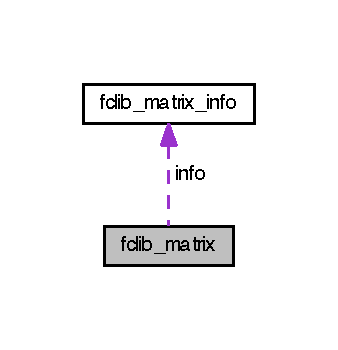
\includegraphics[width=162pt]{structfclib__matrix__coll__graph}
\end{center}
\end{figure}
\subsubsection*{Public Attributes}
\begin{DoxyCompactItemize}
\item 
int \hyperlink{structfclib__matrix_ad59323011143dc70ef74f4377279e0d0}{nzmax}
\begin{DoxyCompactList}\small\item\em maximum number of entries \end{DoxyCompactList}\item 
int \hyperlink{structfclib__matrix_aaec2a835fcc339c3fb84227e2f7b861b}{m}
\begin{DoxyCompactList}\small\item\em number of rows \end{DoxyCompactList}\item 
int \hyperlink{structfclib__matrix_ace0c395ca5da8a4bcc4958a29895c639}{n}
\begin{DoxyCompactList}\small\item\em number of columns \end{DoxyCompactList}\item 
int $\ast$ \hyperlink{structfclib__matrix_ace167d937e3c1bb2558e264aefada841}{p}
\begin{DoxyCompactList}\small\item\em compressed\-: row (size m+1) or column (size n+1) pointers; triplet\-: row indices (size nz) \end{DoxyCompactList}\item 
int $\ast$ \hyperlink{structfclib__matrix_aed86c681657206e7502450e437dba667}{i}
\begin{DoxyCompactList}\small\item\em compressed\-: column or row indices, size nzmax; triplet\-: column indices (size nz) \end{DoxyCompactList}\item 
double $\ast$ \hyperlink{structfclib__matrix_aba1891f51a81f973249456c91715e06d}{x}
\begin{DoxyCompactList}\small\item\em numerical values, size nzmax \end{DoxyCompactList}\item 
int \hyperlink{structfclib__matrix_a7d64a7cddc93a8e1f96ab32e9afe0bbb}{nz}
\begin{DoxyCompactList}\small\item\em \subsubsection*{of entries in triplet matrix, -\/1 for compressed columns, -\/2 for compressed rows}\end{DoxyCompactList}\item 
struct \hyperlink{structfclib__matrix__info}{fclib\-\_\-matrix\-\_\-info} $\ast$ \hyperlink{structfclib__matrix_ac0af227334c5b0a13a3222c8f04add36}{info}
\begin{DoxyCompactList}\small\item\em info for this matrix \end{DoxyCompactList}\end{DoxyCompactItemize}


\subsubsection{Detailed Description}
matrix in compressed row/column or triplet form 

Definition at line 119 of file fclib.\-h.



\subsubsection{Member Data Documentation}
\hypertarget{structfclib__matrix_ad59323011143dc70ef74f4377279e0d0}{\index{fclib\-\_\-matrix@{fclib\-\_\-matrix}!nzmax@{nzmax}}
\index{nzmax@{nzmax}!fclib_matrix@{fclib\-\_\-matrix}}
\paragraph[{nzmax}]{\setlength{\rightskip}{0pt plus 5cm}int fclib\-\_\-matrix\-::nzmax}}\label{structfclib__matrix_ad59323011143dc70ef74f4377279e0d0}


maximum number of entries 



Definition at line 122 of file fclib.\-h.



Referenced by compare\-\_\-matrices(), random\-\_\-matrix(), read\-\_\-matrix(), and write\-\_\-matrix().

\hypertarget{structfclib__matrix_aaec2a835fcc339c3fb84227e2f7b861b}{\index{fclib\-\_\-matrix@{fclib\-\_\-matrix}!m@{m}}
\index{m@{m}!fclib_matrix@{fclib\-\_\-matrix}}
\paragraph[{m}]{\setlength{\rightskip}{0pt plus 5cm}int fclib\-\_\-matrix\-::m}}\label{structfclib__matrix_aaec2a835fcc339c3fb84227e2f7b861b}


number of rows 



Definition at line 124 of file fclib.\-h.



Referenced by compare\-\_\-global\-\_\-problems(), compare\-\_\-matrices(), main(), matrix\-\_\-info(), random\-\_\-matrix(), read\-\_\-global\-\_\-vectors(), read\-\_\-local\-\_\-vectors(), read\-\_\-matrix(), write\-\_\-global\-\_\-vectors(), write\-\_\-local\-\_\-vectors(), and write\-\_\-matrix().

\hypertarget{structfclib__matrix_ace0c395ca5da8a4bcc4958a29895c639}{\index{fclib\-\_\-matrix@{fclib\-\_\-matrix}!n@{n}}
\index{n@{n}!fclib_matrix@{fclib\-\_\-matrix}}
\paragraph[{n}]{\setlength{\rightskip}{0pt plus 5cm}int fclib\-\_\-matrix\-::n}}\label{structfclib__matrix_ace0c395ca5da8a4bcc4958a29895c639}


number of columns 



Definition at line 126 of file fclib.\-h.



Referenced by compare\-\_\-global\-\_\-problems(), compare\-\_\-local\-\_\-problems(), compare\-\_\-matrices(), fclib\-\_\-merit\-\_\-local(), main(), random\-\_\-global\-\_\-problem(), random\-\_\-global\-\_\-solutions(), random\-\_\-local\-\_\-solutions(), random\-\_\-matrix(), read\-\_\-global\-\_\-vectors(), read\-\_\-matrix(), write\-\_\-global\-\_\-vectors(), and write\-\_\-matrix().

\hypertarget{structfclib__matrix_ace167d937e3c1bb2558e264aefada841}{\index{fclib\-\_\-matrix@{fclib\-\_\-matrix}!p@{p}}
\index{p@{p}!fclib_matrix@{fclib\-\_\-matrix}}
\paragraph[{p}]{\setlength{\rightskip}{0pt plus 5cm}int$\ast$ fclib\-\_\-matrix\-::p}}\label{structfclib__matrix_ace167d937e3c1bb2558e264aefada841}


compressed\-: row (size m+1) or column (size n+1) pointers; triplet\-: row indices (size nz) 



Definition at line 128 of file fclib.\-h.



Referenced by compare\-\_\-matrices(), delete\-\_\-matrix(), random\-\_\-matrix(), read\-\_\-matrix(), and write\-\_\-matrix().

\hypertarget{structfclib__matrix_aed86c681657206e7502450e437dba667}{\index{fclib\-\_\-matrix@{fclib\-\_\-matrix}!i@{i}}
\index{i@{i}!fclib_matrix@{fclib\-\_\-matrix}}
\paragraph[{i}]{\setlength{\rightskip}{0pt plus 5cm}int$\ast$ fclib\-\_\-matrix\-::i}}\label{structfclib__matrix_aed86c681657206e7502450e437dba667}


compressed\-: column or row indices, size nzmax; triplet\-: column indices (size nz) 



Definition at line 130 of file fclib.\-h.



Referenced by compare\-\_\-matrices(), delete\-\_\-matrix(), fclib\-\_\-merit\-\_\-local(), random\-\_\-matrix(), read\-\_\-matrix(), and write\-\_\-matrix().

\hypertarget{structfclib__matrix_aba1891f51a81f973249456c91715e06d}{\index{fclib\-\_\-matrix@{fclib\-\_\-matrix}!x@{x}}
\index{x@{x}!fclib_matrix@{fclib\-\_\-matrix}}
\paragraph[{x}]{\setlength{\rightskip}{0pt plus 5cm}double$\ast$ fclib\-\_\-matrix\-::x}}\label{structfclib__matrix_aba1891f51a81f973249456c91715e06d}


numerical values, size nzmax 



Definition at line 132 of file fclib.\-h.



Referenced by compare\-\_\-matrices(), delete\-\_\-matrix(), random\-\_\-matrix(), read\-\_\-matrix(), and write\-\_\-matrix().

\hypertarget{structfclib__matrix_a7d64a7cddc93a8e1f96ab32e9afe0bbb}{\index{fclib\-\_\-matrix@{fclib\-\_\-matrix}!nz@{nz}}
\index{nz@{nz}!fclib_matrix@{fclib\-\_\-matrix}}
\paragraph[{nz}]{\setlength{\rightskip}{0pt plus 5cm}int fclib\-\_\-matrix\-::nz}}\label{structfclib__matrix_a7d64a7cddc93a8e1f96ab32e9afe0bbb}


\subsubsection*{of entries in triplet matrix, -\/1 for compressed columns, -\/2 for compressed rows}



Definition at line 134 of file fclib.\-h.



Referenced by compare\-\_\-matrices(), random\-\_\-matrix(), read\-\_\-matrix(), and write\-\_\-matrix().

\hypertarget{structfclib__matrix_ac0af227334c5b0a13a3222c8f04add36}{\index{fclib\-\_\-matrix@{fclib\-\_\-matrix}!info@{info}}
\index{info@{info}!fclib_matrix@{fclib\-\_\-matrix}}
\paragraph[{info}]{\setlength{\rightskip}{0pt plus 5cm}struct {\bf fclib\-\_\-matrix\-\_\-info}$\ast$ fclib\-\_\-matrix\-::info}}\label{structfclib__matrix_ac0af227334c5b0a13a3222c8f04add36}


info for this matrix 



Definition at line 136 of file fclib.\-h.



Referenced by compare\-\_\-matrices(), delete\-\_\-matrix(), random\-\_\-matrix(), read\-\_\-matrix(), and write\-\_\-matrix().


\hypertarget{structfclib__matrix__info}{\subsection{fclib\-\_\-matrix\-\_\-info Struct Reference}
\label{structfclib__matrix__info}\index{fclib\-\_\-matrix\-\_\-info@{fclib\-\_\-matrix\-\_\-info}}
}


This structure allows the user to enter a description for a given matrix (comment, conditionning, determinant, rank.) if they are known.  




{\ttfamily \#include $<$fclib.\-h$>$}

\subsubsection*{Public Attributes}
\begin{DoxyCompactItemize}
\item 
char $\ast$ \hyperlink{structfclib__matrix__info_a9c4994b1759bf3a7a75c72cd78709722}{comment}
\begin{DoxyCompactList}\small\item\em comment on the matrix properties \end{DoxyCompactList}\item 
double \hyperlink{structfclib__matrix__info_a453db794429411025f2b8dfb497f5f35}{conditioning}
\begin{DoxyCompactList}\small\item\em conditioning \end{DoxyCompactList}\item 
double \hyperlink{structfclib__matrix__info_a9c6697aee458be4494b215f0f003ca48}{determinant}
\begin{DoxyCompactList}\small\item\em determinant \end{DoxyCompactList}\item 
int \hyperlink{structfclib__matrix__info_af838043a1769956958c4a66e6227227d}{rank}
\begin{DoxyCompactList}\small\item\em rank \end{DoxyCompactList}\end{DoxyCompactItemize}


\subsubsection{Detailed Description}
This structure allows the user to enter a description for a given matrix (comment, conditionning, determinant, rank.) if they are known. 

Definition at line 104 of file fclib.\-h.



\subsubsection{Member Data Documentation}
\hypertarget{structfclib__matrix__info_a9c4994b1759bf3a7a75c72cd78709722}{\index{fclib\-\_\-matrix\-\_\-info@{fclib\-\_\-matrix\-\_\-info}!comment@{comment}}
\index{comment@{comment}!fclib_matrix_info@{fclib\-\_\-matrix\-\_\-info}}
\paragraph[{comment}]{\setlength{\rightskip}{0pt plus 5cm}char$\ast$ fclib\-\_\-matrix\-\_\-info\-::comment}}\label{structfclib__matrix__info_a9c4994b1759bf3a7a75c72cd78709722}


comment on the matrix properties 



Definition at line 107 of file fclib.\-h.



Referenced by compare\-\_\-matrix\-\_\-infos(), delete\-\_\-matrix\-\_\-info(), matrix\-\_\-info(), read\-\_\-matrix(), and write\-\_\-matrix().

\hypertarget{structfclib__matrix__info_a453db794429411025f2b8dfb497f5f35}{\index{fclib\-\_\-matrix\-\_\-info@{fclib\-\_\-matrix\-\_\-info}!conditioning@{conditioning}}
\index{conditioning@{conditioning}!fclib_matrix_info@{fclib\-\_\-matrix\-\_\-info}}
\paragraph[{conditioning}]{\setlength{\rightskip}{0pt plus 5cm}double fclib\-\_\-matrix\-\_\-info\-::conditioning}}\label{structfclib__matrix__info_a453db794429411025f2b8dfb497f5f35}


conditioning 



Definition at line 109 of file fclib.\-h.



Referenced by compare\-\_\-matrix\-\_\-infos(), matrix\-\_\-info(), read\-\_\-matrix(), and write\-\_\-matrix().

\hypertarget{structfclib__matrix__info_a9c6697aee458be4494b215f0f003ca48}{\index{fclib\-\_\-matrix\-\_\-info@{fclib\-\_\-matrix\-\_\-info}!determinant@{determinant}}
\index{determinant@{determinant}!fclib_matrix_info@{fclib\-\_\-matrix\-\_\-info}}
\paragraph[{determinant}]{\setlength{\rightskip}{0pt plus 5cm}double fclib\-\_\-matrix\-\_\-info\-::determinant}}\label{structfclib__matrix__info_a9c6697aee458be4494b215f0f003ca48}


determinant 



Definition at line 111 of file fclib.\-h.



Referenced by compare\-\_\-matrix\-\_\-infos(), matrix\-\_\-info(), read\-\_\-matrix(), and write\-\_\-matrix().

\hypertarget{structfclib__matrix__info_af838043a1769956958c4a66e6227227d}{\index{fclib\-\_\-matrix\-\_\-info@{fclib\-\_\-matrix\-\_\-info}!rank@{rank}}
\index{rank@{rank}!fclib_matrix_info@{fclib\-\_\-matrix\-\_\-info}}
\paragraph[{rank}]{\setlength{\rightskip}{0pt plus 5cm}int fclib\-\_\-matrix\-\_\-info\-::rank}}\label{structfclib__matrix__info_af838043a1769956958c4a66e6227227d}


rank 



Definition at line 113 of file fclib.\-h.



Referenced by compare\-\_\-matrix\-\_\-infos(), matrix\-\_\-info(), read\-\_\-matrix(), and write\-\_\-matrix().


\hypertarget{structfclib__solution}{\subsection{fclib\-\_\-solution Struct Reference}
\label{structfclib__solution}\index{fclib\-\_\-solution@{fclib\-\_\-solution}}
}


A solution or a guess for the frictional contact problem.  




{\ttfamily \#include $<$fclib.\-h$>$}

\subsubsection*{Public Attributes}
\begin{DoxyCompactItemize}
\item 
double $\ast$ \hyperlink{structfclib__solution_a252982ce524686a094223a55c194fea8}{v}
\begin{DoxyCompactList}\small\item\em global velocity (or position/displacement for quasi-\/static problems) solution vector \end{DoxyCompactList}\item 
double $\ast$ \hyperlink{structfclib__solution_acb160f0dad04b9420388464d256ae41f}{u}
\begin{DoxyCompactList}\small\item\em local velocity (or position/displacement for quasi-\/static problems) solution vector \end{DoxyCompactList}\item 
double $\ast$ \hyperlink{structfclib__solution_aba0437aebbb1060350ef2f0a6e8b504d}{r}
\begin{DoxyCompactList}\small\item\em local contact forces (or impulses) solution vector \end{DoxyCompactList}\item 
double $\ast$ \hyperlink{structfclib__solution_a872a687856540dd19286aec43d890ede}{l}
\begin{DoxyCompactList}\small\item\em multiplier for equlity constraints ( $\lambda$) solution vector \end{DoxyCompactList}\end{DoxyCompactItemize}


\subsubsection{Detailed Description}
A solution or a guess for the frictional contact problem. 

This structure allows to store a solution vector of a guess vector for the various frictional contact problems. 

Definition at line 254 of file fclib.\-h.



\subsubsection{Member Data Documentation}
\hypertarget{structfclib__solution_a252982ce524686a094223a55c194fea8}{\index{fclib\-\_\-solution@{fclib\-\_\-solution}!v@{v}}
\index{v@{v}!fclib_solution@{fclib\-\_\-solution}}
\paragraph[{v}]{\setlength{\rightskip}{0pt plus 5cm}double$\ast$ fclib\-\_\-solution\-::v}}\label{structfclib__solution_a252982ce524686a094223a55c194fea8}


global velocity (or position/displacement for quasi-\/static problems) solution vector 



Definition at line 257 of file fclib.\-h.



Referenced by compare\-\_\-solutions(), fclib\-\_\-delete\-\_\-solutions(), fclib\-\_\-merit\-\_\-local(), random\-\_\-global\-\_\-solutions(), random\-\_\-local\-\_\-solutions(), read\-\_\-solution(), and write\-\_\-solution().

\hypertarget{structfclib__solution_acb160f0dad04b9420388464d256ae41f}{\index{fclib\-\_\-solution@{fclib\-\_\-solution}!u@{u}}
\index{u@{u}!fclib_solution@{fclib\-\_\-solution}}
\paragraph[{u}]{\setlength{\rightskip}{0pt plus 5cm}double$\ast$ fclib\-\_\-solution\-::u}}\label{structfclib__solution_acb160f0dad04b9420388464d256ae41f}


local velocity (or position/displacement for quasi-\/static problems) solution vector 



Definition at line 259 of file fclib.\-h.



Referenced by compare\-\_\-solutions(), fclib\-\_\-delete\-\_\-solutions(), fclib\-\_\-merit\-\_\-local(), random\-\_\-global\-\_\-solutions(), random\-\_\-local\-\_\-solutions(), read\-\_\-solution(), and write\-\_\-solution().

\hypertarget{structfclib__solution_aba0437aebbb1060350ef2f0a6e8b504d}{\index{fclib\-\_\-solution@{fclib\-\_\-solution}!r@{r}}
\index{r@{r}!fclib_solution@{fclib\-\_\-solution}}
\paragraph[{r}]{\setlength{\rightskip}{0pt plus 5cm}double$\ast$ fclib\-\_\-solution\-::r}}\label{structfclib__solution_aba0437aebbb1060350ef2f0a6e8b504d}


local contact forces (or impulses) solution vector 



Definition at line 261 of file fclib.\-h.



Referenced by compare\-\_\-solutions(), fclib\-\_\-delete\-\_\-solutions(), fclib\-\_\-merit\-\_\-local(), random\-\_\-global\-\_\-solutions(), random\-\_\-local\-\_\-solutions(), read\-\_\-solution(), and write\-\_\-solution().

\hypertarget{structfclib__solution_a872a687856540dd19286aec43d890ede}{\index{fclib\-\_\-solution@{fclib\-\_\-solution}!l@{l}}
\index{l@{l}!fclib_solution@{fclib\-\_\-solution}}
\paragraph[{l}]{\setlength{\rightskip}{0pt plus 5cm}double$\ast$ fclib\-\_\-solution\-::l}}\label{structfclib__solution_a872a687856540dd19286aec43d890ede}


multiplier for equlity constraints ( $\lambda$) solution vector 



Definition at line 263 of file fclib.\-h.



Referenced by compare\-\_\-solutions(), fclib\-\_\-delete\-\_\-solutions(), fclib\-\_\-merit\-\_\-local(), random\-\_\-global\-\_\-solutions(), random\-\_\-local\-\_\-solutions(), read\-\_\-solution(), and write\-\_\-solution().


\section{File Documentation}
\hypertarget{additionalpages_8doxygen}{\subsection{additionalpages.\-doxygen File Reference}
\label{additionalpages_8doxygen}\index{additionalpages.\-doxygen@{additionalpages.\-doxygen}}
}

\hypertarget{csparse_8c}{\subsection{csparse.\-c File Reference}
\label{csparse_8c}\index{csparse.\-c@{csparse.\-c}}
}
{\ttfamily \#include $<$stdlib.\-h$>$}\\*
{\ttfamily \#include $<$limits.\-h$>$}\\*
{\ttfamily \#include $<$math.\-h$>$}\\*
{\ttfamily \#include $<$stdio.\-h$>$}\\*
{\ttfamily \#include \char`\"{}csparse.\-h\char`\"{}}\\*
Include dependency graph for csparse.\-c\-:\nopagebreak
\begin{figure}[H]
\begin{center}
\leavevmode
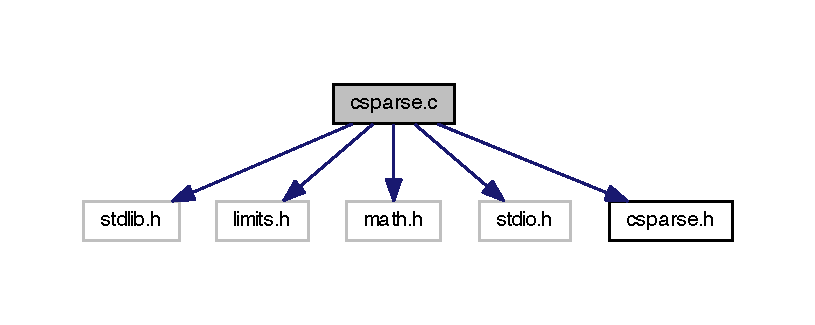
\includegraphics[width=350pt]{csparse_8c__incl}
\end{center}
\end{figure}
\subsubsection*{Functions}
\begin{DoxyCompactItemize}
\item 
\hyperlink{csparse_8h_a44e471a015cf32e012cffef17e81b6db}{cs} $\ast$ \hyperlink{csparse_8c_a12000fbd0b9198d3852978cca8386afe}{cs\-\_\-add} (const \hyperlink{csparse_8h_a44e471a015cf32e012cffef17e81b6db}{cs} $\ast$A, const \hyperlink{csparse_8h_a44e471a015cf32e012cffef17e81b6db}{cs} $\ast$B, double alpha, double beta)
\item 
static int \hyperlink{csparse_8c_a73c323ac388668ef8ab5a2aa97807fbe}{cs\-\_\-wclear} (int mark, int lemax, int $\ast$w, int n)
\item 
static int \hyperlink{csparse_8c_ab744b6c0bb84f8f54496c547e8a95e16}{cs\-\_\-diag} (int i, int j, double aij, void $\ast$other)
\item 
int $\ast$ \hyperlink{csparse_8c_a8ae6ef945b48ea6aff888481c8394ef8}{cs\-\_\-amd} (const \hyperlink{csparse_8h_a44e471a015cf32e012cffef17e81b6db}{cs} $\ast$A, int order)
\item 
static int \hyperlink{csparse_8c_a48e5697b039da6a7bfff8dc91cc7bfc4}{cs\-\_\-ereach} (const \hyperlink{csparse_8h_a44e471a015cf32e012cffef17e81b6db}{cs} $\ast$A, int k, const int $\ast$parent, int $\ast$s, int $\ast$w, double $\ast$x, int top)
\item 
\hyperlink{csparse_8h_aa81f48a471a94557a00da42ceb21dc68}{csn} $\ast$ \hyperlink{csparse_8c_a5ae664f3c6b2baeed717be084e00e13f}{cs\-\_\-chol} (const \hyperlink{csparse_8h_a44e471a015cf32e012cffef17e81b6db}{cs} $\ast$A, const \hyperlink{csparse_8h_afdd66916fadd9fd39cd279717aa5c6b9}{css} $\ast$S)
\item 
int \hyperlink{csparse_8c_ac3a64b3dfa45b30d2e764e096107ba1e}{cs\-\_\-cholsol} (const \hyperlink{csparse_8h_a44e471a015cf32e012cffef17e81b6db}{cs} $\ast$A, double $\ast$b, int order)
\item 
static void \hyperlink{csparse_8c_a81c80549e731339bf1dc4b55d0195544}{cs\-\_\-cedge} (int j, int i, const int $\ast$first, int $\ast$maxfirst, int $\ast$delta, int $\ast$prevleaf, int $\ast$ancestor)
\item 
int $\ast$ \hyperlink{csparse_8c_aa7fdeead97aef81cdf18af7576a7f722}{cs\-\_\-counts} (const \hyperlink{csparse_8h_a44e471a015cf32e012cffef17e81b6db}{cs} $\ast$A, const int $\ast$parent, const int $\ast$post, int ata)
\item 
int \hyperlink{csparse_8c_afa16a8bc0209e3bd5c0819ed15d2c987}{cs\-\_\-cumsum} (int $\ast$p, int $\ast$c, int n)
\item 
int \hyperlink{csparse_8c_a30e23f78c9bcbe87e9027d078c98467a}{cs\-\_\-dfs} (int j, \hyperlink{csparse_8h_a44e471a015cf32e012cffef17e81b6db}{cs} $\ast$L, int top, int $\ast$xi, int $\ast$pstack, const int $\ast$Pinv)
\item 
static int \hyperlink{csparse_8c_ae296f1a9ad0b70efedc382fae12e028b}{cs\-\_\-bfs} (const \hyperlink{csparse_8h_a44e471a015cf32e012cffef17e81b6db}{cs} $\ast$A, int n, int $\ast$wi, int $\ast$wj, int $\ast$queue, const int $\ast$imatch, const int $\ast$jmatch, int mark)
\item 
static void \hyperlink{csparse_8c_a1a8f474b45442c314cadf760871433c3}{cs\-\_\-matched} (int m, const int $\ast$wi, const int $\ast$jmatch, int $\ast$P, int $\ast$Q, int $\ast$cc, int $\ast$rr, int set, int mark)
\item 
static void \hyperlink{csparse_8c_af3bc55de536690597bfefa13d827bcb5}{cs\-\_\-unmatched} (int m, const int $\ast$wi, int $\ast$P, int $\ast$rr, int set)
\item 
static int \hyperlink{csparse_8c_ab71ee855eb5dc6e1aa6f0de6a4253d87}{cs\-\_\-rprune} (int i, int j, double aij, void $\ast$other)
\item 
\hyperlink{csparse_8h_a157bda8b8156601179bd598e17ff4b9d}{csd} $\ast$ \hyperlink{csparse_8c_a59484c944748596c1a9adecfd19085b4}{cs\-\_\-dmperm} (const \hyperlink{csparse_8h_a44e471a015cf32e012cffef17e81b6db}{cs} $\ast$A)
\item 
static int \hyperlink{csparse_8c_adb704422b5f80f757920bf30c5dcabed}{cs\-\_\-tol} (int i, int j, double aij, void $\ast$tol)
\item 
int \hyperlink{csparse_8c_a39d53ef3034685545cda58ae28af6bb5}{cs\-\_\-droptol} (\hyperlink{csparse_8h_a44e471a015cf32e012cffef17e81b6db}{cs} $\ast$A, double tol)
\item 
static int \hyperlink{csparse_8c_a9dad9370bdde743eee26de2d53572bda}{cs\-\_\-nonzero} (int i, int j, double aij, void $\ast$other)
\item 
int \hyperlink{csparse_8c_a50c30e47141ef37dbb4b342e1b4ba924}{cs\-\_\-dropzeros} (\hyperlink{csparse_8h_a44e471a015cf32e012cffef17e81b6db}{cs} $\ast$A)
\item 
int \hyperlink{csparse_8c_a83dc83954d821b748c3ba9fea1f6b5ca}{cs\-\_\-dupl} (\hyperlink{csparse_8h_a44e471a015cf32e012cffef17e81b6db}{cs} $\ast$A)
\item 
int \hyperlink{csparse_8c_a123f77ef9b940089a931a994deb21735}{cs\-\_\-entry} (\hyperlink{csparse_8h_a44e471a015cf32e012cffef17e81b6db}{cs} $\ast$T, int i, int j, double x)
\item 
int $\ast$ \hyperlink{csparse_8c_a5c531804008e67c207e93f14c2551b1a}{cs\-\_\-etree} (const \hyperlink{csparse_8h_a44e471a015cf32e012cffef17e81b6db}{cs} $\ast$A, int ata)
\item 
int \hyperlink{csparse_8c_ade63a58ec1758250c64518d817ea3c4c}{cs\-\_\-fkeep} (\hyperlink{csparse_8h_a44e471a015cf32e012cffef17e81b6db}{cs} $\ast$A, int($\ast$fkeep)(int, int, double, void $\ast$), void $\ast$other)
\item 
int \hyperlink{csparse_8c_a7c887151e9bd6dd56f580c8ae6a5af31}{cs\-\_\-gaxpy} (const \hyperlink{csparse_8h_a44e471a015cf32e012cffef17e81b6db}{cs} $\ast$A, const double $\ast$x, double $\ast$y)
\item 
int \hyperlink{csparse_8c_a27050a31d36046e833b7763fe8ef62ce}{cs\-\_\-happly} (const \hyperlink{csparse_8h_a44e471a015cf32e012cffef17e81b6db}{cs} $\ast$V, int i, double beta, double $\ast$x)
\item 
double \hyperlink{csparse_8c_a096c9057bf2038f9eaef0c1dfb09f3dd}{cs\-\_\-house} (double $\ast$x, double $\ast$beta, int n)
\item 
int \hyperlink{csparse_8c_a51a8d1a79477ff438a978ab1d8f9849b}{cs\-\_\-ipvec} (int n, const int $\ast$P, const double $\ast$b, double $\ast$x)
\item 
\hyperlink{csparse_8h_a44e471a015cf32e012cffef17e81b6db}{cs} $\ast$ \hyperlink{csparse_8c_a12eb66c4f53e51ee5e03ec0b9f24b368}{cs\-\_\-load} (F\-I\-L\-E $\ast$f)
\item 
int \hyperlink{csparse_8c_adbd011bdb4d7bef9825ca1c743fc6b46}{cs\-\_\-lsolve} (const \hyperlink{csparse_8h_a44e471a015cf32e012cffef17e81b6db}{cs} $\ast$L, double $\ast$x)
\item 
int \hyperlink{csparse_8c_afc61741ee2f33a3544f1c5f6b9caf9f6}{cs\-\_\-ltsolve} (const \hyperlink{csparse_8h_a44e471a015cf32e012cffef17e81b6db}{cs} $\ast$L, double $\ast$x)
\item 
\hyperlink{csparse_8h_aa81f48a471a94557a00da42ceb21dc68}{csn} $\ast$ \hyperlink{csparse_8c_a6a35ad4816f210234a33eed09b19d181}{cs\-\_\-lu} (const \hyperlink{csparse_8h_a44e471a015cf32e012cffef17e81b6db}{cs} $\ast$A, const \hyperlink{csparse_8h_afdd66916fadd9fd39cd279717aa5c6b9}{css} $\ast$S, double tol)
\item 
int \hyperlink{csparse_8c_a14612df0010f5284c8f3feac2a7e02fd}{cs\-\_\-lusol} (const \hyperlink{csparse_8h_a44e471a015cf32e012cffef17e81b6db}{cs} $\ast$A, double $\ast$b, int order, double tol)
\item 
void $\ast$ \hyperlink{csparse_8c_a4c6c75c54cbdf2f3fd4574a90c2f8a86}{cs\-\_\-malloc} (int n, size\-\_\-t size)
\item 
void $\ast$ \hyperlink{csparse_8c_ad3e846c0142a1457e8e85bcaf559fb98}{cs\-\_\-calloc} (int n, size\-\_\-t size)
\item 
void $\ast$ \hyperlink{csparse_8c_a78c1d1194aacc65212bb0d2b03643ac7}{cs\-\_\-free} (void $\ast$p)
\item 
void $\ast$ \hyperlink{csparse_8c_a7e829e1175f2c8ddb0d6d9e0bb90f985}{cs\-\_\-realloc} (void $\ast$p, int n, size\-\_\-t size, int $\ast$ok)
\item 
static void \hyperlink{csparse_8c_a76ac84cfd998800844b585a556a5f6ad}{cs\-\_\-augment} (int k, const \hyperlink{csparse_8h_a44e471a015cf32e012cffef17e81b6db}{cs} $\ast$A, int $\ast$jmatch, int $\ast$cheap, int $\ast$w, int $\ast$js, int $\ast$is, int $\ast$ps)
\item 
int $\ast$ \hyperlink{csparse_8c_aebd7035aaa1627313149c32755b9f642}{cs\-\_\-maxtrans} (const \hyperlink{csparse_8h_a44e471a015cf32e012cffef17e81b6db}{cs} $\ast$A)
\item 
\hyperlink{csparse_8h_a44e471a015cf32e012cffef17e81b6db}{cs} $\ast$ \hyperlink{csparse_8c_a066e18f8570c820530c73ebc88b30a97}{cs\-\_\-multiply} (const \hyperlink{csparse_8h_a44e471a015cf32e012cffef17e81b6db}{cs} $\ast$A, const \hyperlink{csparse_8h_a44e471a015cf32e012cffef17e81b6db}{cs} $\ast$B)
\item 
double \hyperlink{csparse_8c_ae2b324f8f0cdc3610d98ce6cebd50075}{cs\-\_\-norm} (const \hyperlink{csparse_8h_a44e471a015cf32e012cffef17e81b6db}{cs} $\ast$A)
\item 
\hyperlink{csparse_8h_a44e471a015cf32e012cffef17e81b6db}{cs} $\ast$ \hyperlink{csparse_8c_a752362fe7bf8d0d49d3c2d788f4d38a9}{cs\-\_\-permute} (const \hyperlink{csparse_8h_a44e471a015cf32e012cffef17e81b6db}{cs} $\ast$A, const int $\ast$Pinv, const int $\ast$Q, int values)
\item 
int $\ast$ \hyperlink{csparse_8c_af29c4a6ca5cea4b9ffa1cbf24636bbc6}{cs\-\_\-pinv} (int const $\ast$P, int n)
\item 
int $\ast$ \hyperlink{csparse_8c_af84bc0a35c099a9a1e01e5aebf8c7292}{cs\-\_\-post} (int n, const int $\ast$parent)
\item 
int \hyperlink{csparse_8c_ab3e2c74ed6cf7521170a45d04aab9b51}{cs\-\_\-print} (const \hyperlink{csparse_8h_a44e471a015cf32e012cffef17e81b6db}{cs} $\ast$A, int brief)
\item 
int \hyperlink{csparse_8c_a547d4d67ec772ecf190dc7073e7fcf41}{cs\-\_\-pvec} (int n, const int $\ast$P, const double $\ast$b, double $\ast$x)
\item 
\hyperlink{csparse_8h_aa81f48a471a94557a00da42ceb21dc68}{csn} $\ast$ \hyperlink{csparse_8c_a767dc90c22d90fe898f72c2da0d98c03}{cs\-\_\-qr} (const \hyperlink{csparse_8h_a44e471a015cf32e012cffef17e81b6db}{cs} $\ast$A, const \hyperlink{csparse_8h_afdd66916fadd9fd39cd279717aa5c6b9}{css} $\ast$S)
\item 
int \hyperlink{csparse_8c_a833a289a30d66ea255d49ab3e93c1334}{cs\-\_\-qrsol} (const \hyperlink{csparse_8h_a44e471a015cf32e012cffef17e81b6db}{cs} $\ast$A, double $\ast$b, int order)
\item 
int \hyperlink{csparse_8c_add4fc69b3887fae610e0362fc13bb214}{cs\-\_\-reach} (\hyperlink{csparse_8h_a44e471a015cf32e012cffef17e81b6db}{cs} $\ast$L, const \hyperlink{csparse_8h_a44e471a015cf32e012cffef17e81b6db}{cs} $\ast$B, int k, int $\ast$xi, const int $\ast$Pinv)
\item 
int \hyperlink{csparse_8c_a3729a7e21dbc3309ac96461ddb060328}{cs\-\_\-scatter} (const \hyperlink{csparse_8h_a44e471a015cf32e012cffef17e81b6db}{cs} $\ast$A, int j, double beta, int $\ast$w, double $\ast$x, int mark, \hyperlink{csparse_8h_a44e471a015cf32e012cffef17e81b6db}{cs} $\ast$C, int nz)
\item 
\hyperlink{csparse_8h_a157bda8b8156601179bd598e17ff4b9d}{csd} $\ast$ \hyperlink{csparse_8c_a9fede5f7dcf4367d7d005ca6dd0ba100}{cs\-\_\-scc} (\hyperlink{csparse_8h_a44e471a015cf32e012cffef17e81b6db}{cs} $\ast$A)
\item 
\hyperlink{csparse_8h_afdd66916fadd9fd39cd279717aa5c6b9}{css} $\ast$ \hyperlink{csparse_8c_afcc0ebf37f4cf80e097ac7e8aa2830f2}{cs\-\_\-schol} (const \hyperlink{csparse_8h_a44e471a015cf32e012cffef17e81b6db}{cs} $\ast$A, int order)
\item 
int \hyperlink{csparse_8c_aabed11053c84c540d80e6edc410cce2f}{cs\-\_\-splsolve} (\hyperlink{csparse_8h_a44e471a015cf32e012cffef17e81b6db}{cs} $\ast$L, const \hyperlink{csparse_8h_a44e471a015cf32e012cffef17e81b6db}{cs} $\ast$B, int k, int $\ast$xi, double $\ast$x, const int $\ast$Pinv)
\item 
static int $\ast$ \hyperlink{csparse_8c_a205fe209b778ab1379668d9037f1e6d7}{cs\-\_\-vcount} (const \hyperlink{csparse_8h_a44e471a015cf32e012cffef17e81b6db}{cs} $\ast$A, const int $\ast$parent, int $\ast$m2, int $\ast$vnz)
\item 
\hyperlink{csparse_8h_afdd66916fadd9fd39cd279717aa5c6b9}{css} $\ast$ \hyperlink{csparse_8c_a0a717b429d68d3c98b6dc8579988473d}{cs\-\_\-sqr} (const \hyperlink{csparse_8h_a44e471a015cf32e012cffef17e81b6db}{cs} $\ast$A, int order, int qr)
\item 
\hyperlink{csparse_8h_a44e471a015cf32e012cffef17e81b6db}{cs} $\ast$ \hyperlink{csparse_8c_a6aa95f82cd0d8c61afb033405320d727}{cs\-\_\-symperm} (const \hyperlink{csparse_8h_a44e471a015cf32e012cffef17e81b6db}{cs} $\ast$A, const int $\ast$Pinv, int values)
\item 
int \hyperlink{csparse_8c_a7b064c4799cc09da13c13d982197eff7}{cs\-\_\-tdfs} (int j, int k, int $\ast$head, const int $\ast$next, int $\ast$post, int $\ast$stack)
\item 
\hyperlink{csparse_8h_a44e471a015cf32e012cffef17e81b6db}{cs} $\ast$ \hyperlink{csparse_8c_a090225477a18abe5f8d5ab26e4efaf3a}{cs\-\_\-transpose} (const \hyperlink{csparse_8h_a44e471a015cf32e012cffef17e81b6db}{cs} $\ast$A, int values)
\item 
\hyperlink{csparse_8h_a44e471a015cf32e012cffef17e81b6db}{cs} $\ast$ \hyperlink{csparse_8c_a333e20a0edc2af41f68d77d79ede53e5}{cs\-\_\-triplet} (const \hyperlink{csparse_8h_a44e471a015cf32e012cffef17e81b6db}{cs} $\ast$T)
\item 
int \hyperlink{csparse_8c_ad5fa81f80009c06259a77fd7d2092f78}{cs\-\_\-updown} (\hyperlink{csparse_8h_a44e471a015cf32e012cffef17e81b6db}{cs} $\ast$L, int sigma, const \hyperlink{csparse_8h_a44e471a015cf32e012cffef17e81b6db}{cs} $\ast$C, const int $\ast$parent)
\item 
int \hyperlink{csparse_8c_aa4cdacecec403b30b97abc7c27594b4f}{cs\-\_\-usolve} (const \hyperlink{csparse_8h_a44e471a015cf32e012cffef17e81b6db}{cs} $\ast$U, double $\ast$x)
\item 
\hyperlink{csparse_8h_a44e471a015cf32e012cffef17e81b6db}{cs} $\ast$ \hyperlink{csparse_8c_aad3a584d9185a4fe4497a36f892b9c72}{cs\-\_\-spalloc} (int m, int n, int nzmax, int values, int triplet)
\item 
int \hyperlink{csparse_8c_a5a9bc4224732ce1cedc50119afc687c1}{cs\-\_\-sprealloc} (\hyperlink{csparse_8h_a44e471a015cf32e012cffef17e81b6db}{cs} $\ast$A, int nzmax)
\item 
\hyperlink{csparse_8h_a44e471a015cf32e012cffef17e81b6db}{cs} $\ast$ \hyperlink{csparse_8c_a6d705e404a7831ccf01bc0ea064215b9}{cs\-\_\-spfree} (\hyperlink{csparse_8h_a44e471a015cf32e012cffef17e81b6db}{cs} $\ast$A)
\item 
\hyperlink{csparse_8h_aa81f48a471a94557a00da42ceb21dc68}{csn} $\ast$ \hyperlink{csparse_8c_af2e6d75dfc24a842fdbce3aa510dc4bc}{cs\-\_\-nfree} (\hyperlink{csparse_8h_aa81f48a471a94557a00da42ceb21dc68}{csn} $\ast$N)
\item 
\hyperlink{csparse_8h_afdd66916fadd9fd39cd279717aa5c6b9}{css} $\ast$ \hyperlink{csparse_8c_ace766075ef439ad6e4347f6b076eb4b7}{cs\-\_\-sfree} (\hyperlink{csparse_8h_afdd66916fadd9fd39cd279717aa5c6b9}{css} $\ast$S)
\item 
\hyperlink{csparse_8h_a157bda8b8156601179bd598e17ff4b9d}{csd} $\ast$ \hyperlink{csparse_8c_aefbcfeb2d1143578988d22d116dde57b}{cs\-\_\-dalloc} (int m, int n)
\item 
\hyperlink{csparse_8h_a157bda8b8156601179bd598e17ff4b9d}{csd} $\ast$ \hyperlink{csparse_8c_a7c59264397d2c5cc85c87c879aedc4f5}{cs\-\_\-dfree} (\hyperlink{csparse_8h_a157bda8b8156601179bd598e17ff4b9d}{csd} $\ast$D)
\item 
\hyperlink{csparse_8h_a44e471a015cf32e012cffef17e81b6db}{cs} $\ast$ \hyperlink{csparse_8c_a41590e7ef8c8f3ebce8c7bbe07303c28}{cs\-\_\-done} (\hyperlink{csparse_8h_a44e471a015cf32e012cffef17e81b6db}{cs} $\ast$C, void $\ast$w, void $\ast$x, int ok)
\item 
int $\ast$ \hyperlink{csparse_8c_a9c3bd8e36cdfb832d199b580e22467c7}{cs\-\_\-idone} (int $\ast$p, \hyperlink{csparse_8h_a44e471a015cf32e012cffef17e81b6db}{cs} $\ast$C, void $\ast$w, int ok)
\item 
\hyperlink{csparse_8h_aa81f48a471a94557a00da42ceb21dc68}{csn} $\ast$ \hyperlink{csparse_8c_a24796e2f78414578fd2b8e7528535cbb}{cs\-\_\-ndone} (\hyperlink{csparse_8h_aa81f48a471a94557a00da42ceb21dc68}{csn} $\ast$N, \hyperlink{csparse_8h_a44e471a015cf32e012cffef17e81b6db}{cs} $\ast$C, void $\ast$w, void $\ast$x, int ok)
\item 
\hyperlink{csparse_8h_a157bda8b8156601179bd598e17ff4b9d}{csd} $\ast$ \hyperlink{csparse_8c_a312cb23797ac49cd9e99853f6bd2895f}{cs\-\_\-ddone} (\hyperlink{csparse_8h_a157bda8b8156601179bd598e17ff4b9d}{csd} $\ast$D, \hyperlink{csparse_8h_a44e471a015cf32e012cffef17e81b6db}{cs} $\ast$C, void $\ast$w, int ok)
\item 
int \hyperlink{csparse_8c_a9fbb54471515f219326666ffc4e3e255}{cs\-\_\-utsolve} (const \hyperlink{csparse_8h_a44e471a015cf32e012cffef17e81b6db}{cs} $\ast$U, double $\ast$x)
\end{DoxyCompactItemize}


\subsubsection{Function Documentation}
\hypertarget{csparse_8c_a12000fbd0b9198d3852978cca8386afe}{\index{csparse.\-c@{csparse.\-c}!cs\-\_\-add@{cs\-\_\-add}}
\index{cs\-\_\-add@{cs\-\_\-add}!csparse.c@{csparse.\-c}}
\paragraph[{cs\-\_\-add}]{\setlength{\rightskip}{0pt plus 5cm}{\bf cs}$\ast$ cs\-\_\-add (
\begin{DoxyParamCaption}
\item[{const {\bf cs} $\ast$}]{A, }
\item[{const {\bf cs} $\ast$}]{B, }
\item[{double}]{alpha, }
\item[{double}]{beta}
\end{DoxyParamCaption}
)}}\label{csparse_8c_a12000fbd0b9198d3852978cca8386afe}


Definition at line 8 of file csparse.\-c.



References cs\-\_\-calloc(), cs\-\_\-done(), cs\-\_\-malloc(), cs\-\_\-scatter(), cs\-\_\-spalloc(), cs\-\_\-sprealloc(), cs\-\_\-sparse\-::m, cs\-\_\-sparse\-::n, cs\-\_\-sparse\-::p, and cs\-\_\-sparse\-::x.



Referenced by cs\-\_\-amd().



Here is the call graph for this function\-:\nopagebreak
\begin{figure}[H]
\begin{center}
\leavevmode
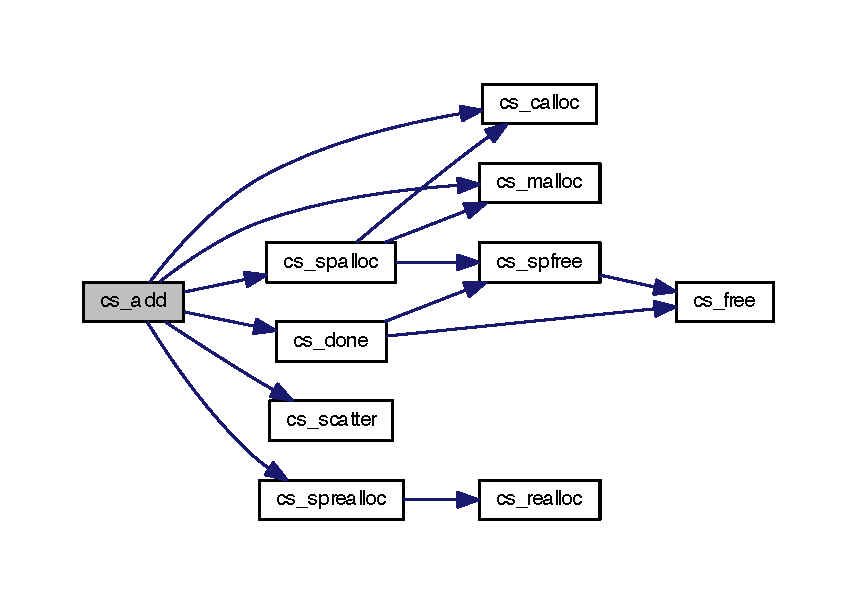
\includegraphics[width=350pt]{csparse_8c_a12000fbd0b9198d3852978cca8386afe_cgraph}
\end{center}
\end{figure}


\hypertarget{csparse_8c_a73c323ac388668ef8ab5a2aa97807fbe}{\index{csparse.\-c@{csparse.\-c}!cs\-\_\-wclear@{cs\-\_\-wclear}}
\index{cs\-\_\-wclear@{cs\-\_\-wclear}!csparse.c@{csparse.\-c}}
\paragraph[{cs\-\_\-wclear}]{\setlength{\rightskip}{0pt plus 5cm}static int cs\-\_\-wclear (
\begin{DoxyParamCaption}
\item[{int}]{mark, }
\item[{int}]{lemax, }
\item[{int $\ast$}]{w, }
\item[{int}]{n}
\end{DoxyParamCaption}
)\hspace{0.3cm}{\ttfamily [static]}}}\label{csparse_8c_a73c323ac388668ef8ab5a2aa97807fbe}


Definition at line 50 of file csparse.\-c.



Referenced by cs\-\_\-amd().

\hypertarget{csparse_8c_ab744b6c0bb84f8f54496c547e8a95e16}{\index{csparse.\-c@{csparse.\-c}!cs\-\_\-diag@{cs\-\_\-diag}}
\index{cs\-\_\-diag@{cs\-\_\-diag}!csparse.c@{csparse.\-c}}
\paragraph[{cs\-\_\-diag}]{\setlength{\rightskip}{0pt plus 5cm}static int cs\-\_\-diag (
\begin{DoxyParamCaption}
\item[{int}]{i, }
\item[{int}]{j, }
\item[{double}]{aij, }
\item[{void $\ast$}]{other}
\end{DoxyParamCaption}
)\hspace{0.3cm}{\ttfamily [static]}}}\label{csparse_8c_ab744b6c0bb84f8f54496c547e8a95e16}


Definition at line 73 of file csparse.\-c.



Referenced by cs\-\_\-amd().

\hypertarget{csparse_8c_a8ae6ef945b48ea6aff888481c8394ef8}{\index{csparse.\-c@{csparse.\-c}!cs\-\_\-amd@{cs\-\_\-amd}}
\index{cs\-\_\-amd@{cs\-\_\-amd}!csparse.c@{csparse.\-c}}
\paragraph[{cs\-\_\-amd}]{\setlength{\rightskip}{0pt plus 5cm}int$\ast$ cs\-\_\-amd (
\begin{DoxyParamCaption}
\item[{const {\bf cs} $\ast$}]{A, }
\item[{int}]{order}
\end{DoxyParamCaption}
)}}\label{csparse_8c_a8ae6ef945b48ea6aff888481c8394ef8}


Definition at line 79 of file csparse.\-c.



References cs\-\_\-add(), cs\-\_\-diag(), cs\-\_\-fkeep(), C\-S\-\_\-\-F\-L\-I\-P, cs\-\_\-idone(), cs\-\_\-malloc(), C\-S\-\_\-\-M\-A\-X, C\-S\-\_\-\-M\-I\-N, cs\-\_\-multiply(), cs\-\_\-spfree(), cs\-\_\-sprealloc(), cs\-\_\-tdfs(), cs\-\_\-transpose(), cs\-\_\-wclear(), cs\-\_\-sparse\-::i, cs\-\_\-sparse\-::m, cs\-\_\-sparse\-::n, cs\-\_\-sparse\-::nzmax, and cs\-\_\-sparse\-::p.



Referenced by cs\-\_\-schol(), and cs\-\_\-sqr().



Here is the call graph for this function\-:\nopagebreak
\begin{figure}[H]
\begin{center}
\leavevmode
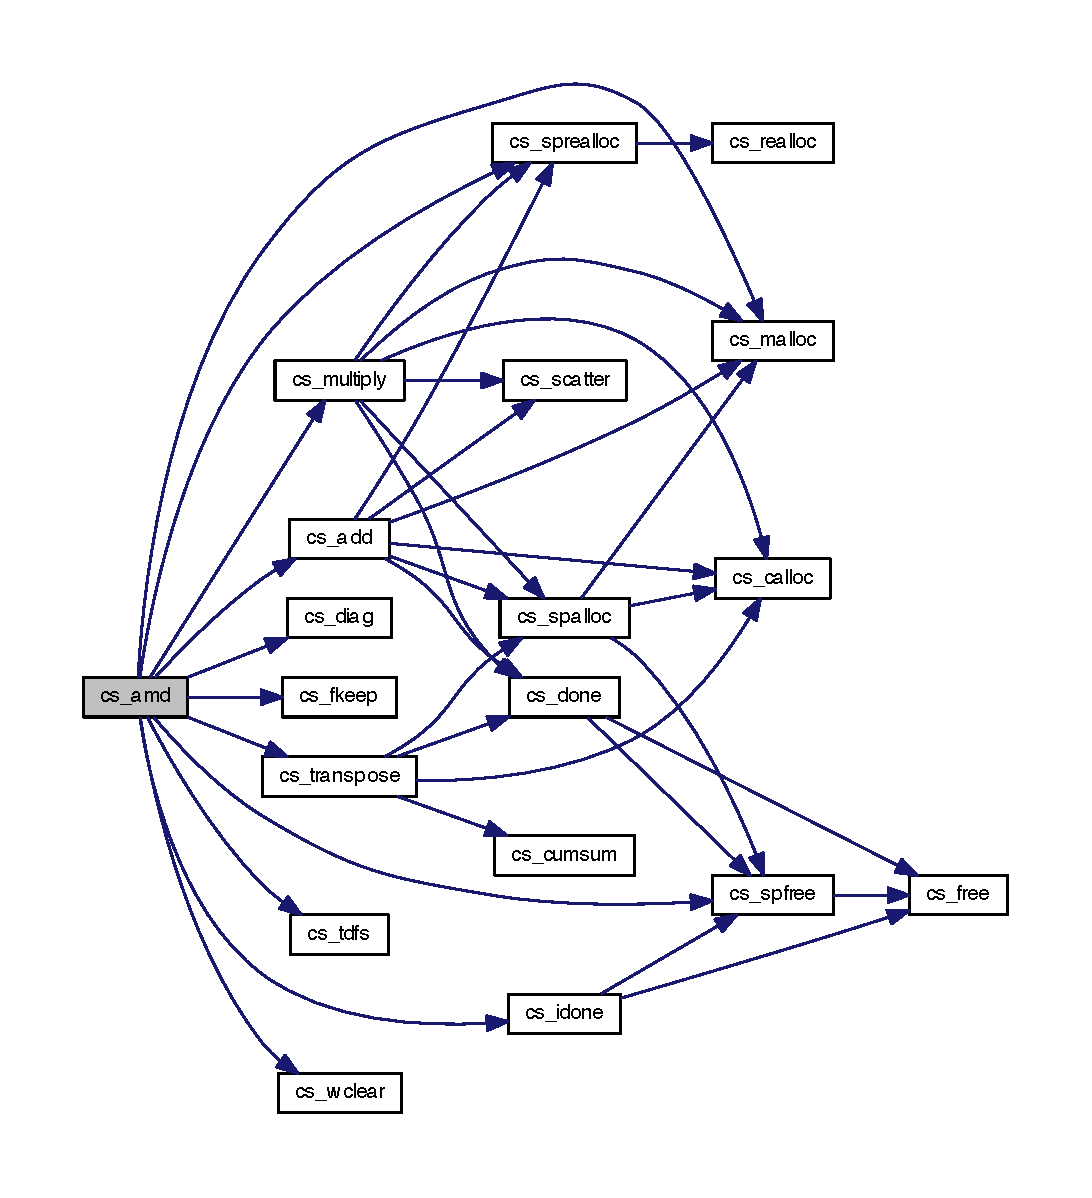
\includegraphics[width=350pt]{csparse_8c_a8ae6ef945b48ea6aff888481c8394ef8_cgraph}
\end{center}
\end{figure}


\hypertarget{csparse_8c_a48e5697b039da6a7bfff8dc91cc7bfc4}{\index{csparse.\-c@{csparse.\-c}!cs\-\_\-ereach@{cs\-\_\-ereach}}
\index{cs\-\_\-ereach@{cs\-\_\-ereach}!csparse.c@{csparse.\-c}}
\paragraph[{cs\-\_\-ereach}]{\setlength{\rightskip}{0pt plus 5cm}static int cs\-\_\-ereach (
\begin{DoxyParamCaption}
\item[{const {\bf cs} $\ast$}]{A, }
\item[{int}]{k, }
\item[{const int $\ast$}]{parent, }
\item[{int $\ast$}]{s, }
\item[{int $\ast$}]{w, }
\item[{double $\ast$}]{x, }
\item[{int}]{top}
\end{DoxyParamCaption}
)\hspace{0.3cm}{\ttfamily [static]}}}\label{csparse_8c_a48e5697b039da6a7bfff8dc91cc7bfc4}


Definition at line 453 of file csparse.\-c.



References cs\-\_\-sparse\-::i, cs\-\_\-sparse\-::p, and cs\-\_\-sparse\-::x.



Referenced by cs\-\_\-chol().

\hypertarget{csparse_8c_a5ae664f3c6b2baeed717be084e00e13f}{\index{csparse.\-c@{csparse.\-c}!cs\-\_\-chol@{cs\-\_\-chol}}
\index{cs\-\_\-chol@{cs\-\_\-chol}!csparse.c@{csparse.\-c}}
\paragraph[{cs\-\_\-chol}]{\setlength{\rightskip}{0pt plus 5cm}{\bf csn}$\ast$ cs\-\_\-chol (
\begin{DoxyParamCaption}
\item[{const {\bf cs} $\ast$}]{A, }
\item[{const {\bf css} $\ast$}]{S}
\end{DoxyParamCaption}
)}}\label{csparse_8c_a5ae664f3c6b2baeed717be084e00e13f}


Definition at line 474 of file csparse.\-c.



References cs\-\_\-symbolic\-::cp, cs\-\_\-calloc(), cs\-\_\-ereach(), cs\-\_\-malloc(), cs\-\_\-ndone(), cs\-\_\-spalloc(), cs\-\_\-symperm(), cs\-\_\-sparse\-::i, cs\-\_\-numeric\-::\-L, cs\-\_\-sparse\-::n, cs\-\_\-sparse\-::p, cs\-\_\-symbolic\-::parent, cs\-\_\-symbolic\-::\-Pinv, and cs\-\_\-sparse\-::x.



Referenced by cs\-\_\-cholsol().



Here is the call graph for this function\-:\nopagebreak
\begin{figure}[H]
\begin{center}
\leavevmode
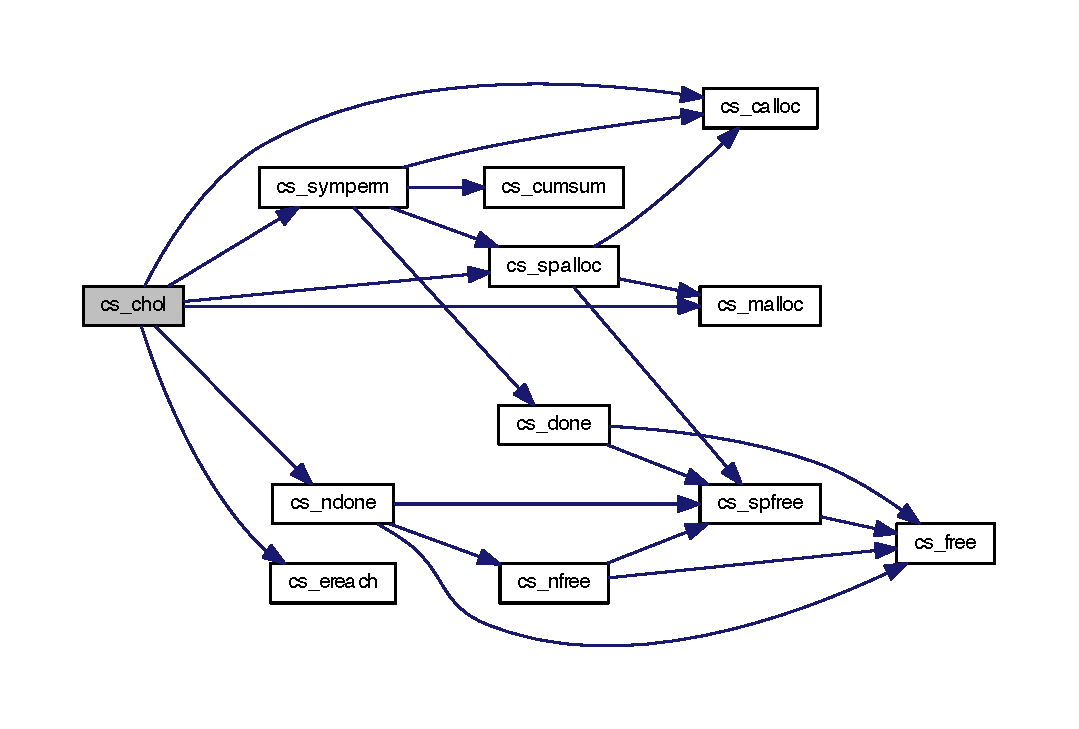
\includegraphics[width=350pt]{csparse_8c_a5ae664f3c6b2baeed717be084e00e13f_cgraph}
\end{center}
\end{figure}


\hypertarget{csparse_8c_ac3a64b3dfa45b30d2e764e096107ba1e}{\index{csparse.\-c@{csparse.\-c}!cs\-\_\-cholsol@{cs\-\_\-cholsol}}
\index{cs\-\_\-cholsol@{cs\-\_\-cholsol}!csparse.c@{csparse.\-c}}
\paragraph[{cs\-\_\-cholsol}]{\setlength{\rightskip}{0pt plus 5cm}int cs\-\_\-cholsol (
\begin{DoxyParamCaption}
\item[{const {\bf cs} $\ast$}]{A, }
\item[{double $\ast$}]{b, }
\item[{int}]{order}
\end{DoxyParamCaption}
)}}\label{csparse_8c_ac3a64b3dfa45b30d2e764e096107ba1e}


Definition at line 533 of file csparse.\-c.



References cs\-\_\-chol(), cs\-\_\-free(), cs\-\_\-ipvec(), cs\-\_\-lsolve(), cs\-\_\-ltsolve(), cs\-\_\-malloc(), cs\-\_\-nfree(), cs\-\_\-pvec(), cs\-\_\-schol(), cs\-\_\-sfree(), cs\-\_\-numeric\-::\-L, cs\-\_\-sparse\-::n, and cs\-\_\-symbolic\-::\-Pinv.



Here is the call graph for this function\-:\nopagebreak
\begin{figure}[H]
\begin{center}
\leavevmode
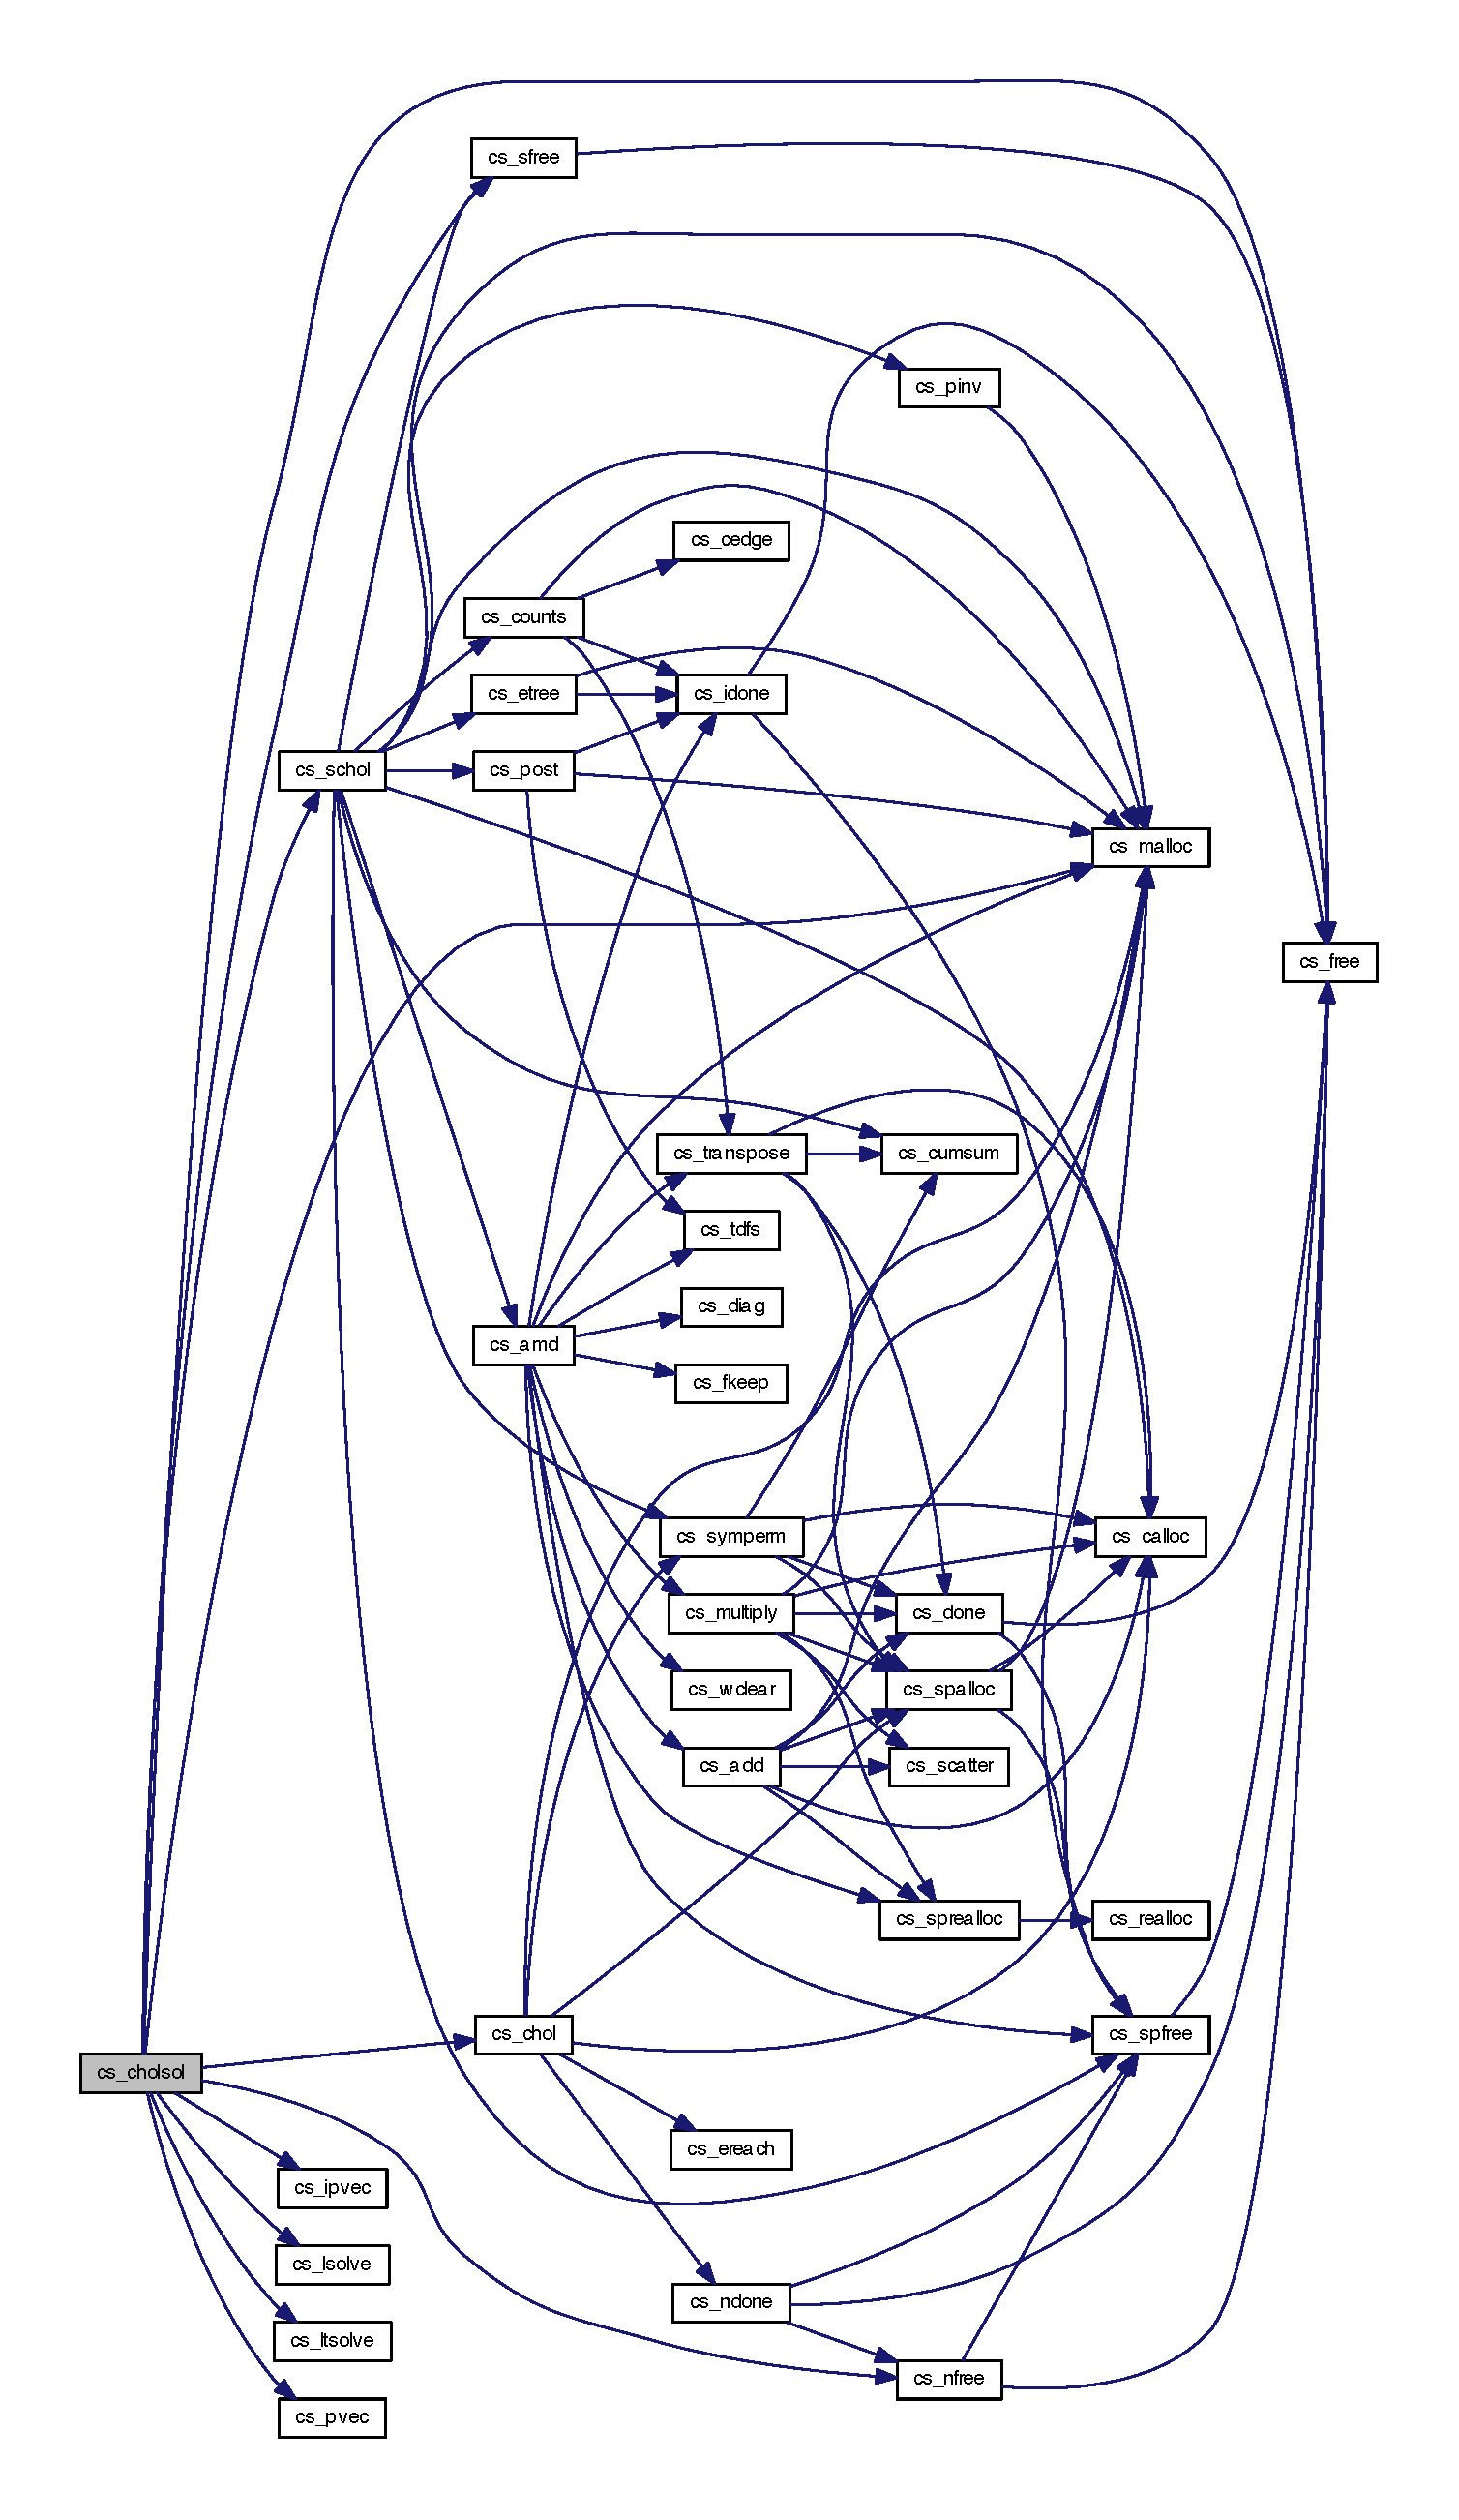
\includegraphics[height=550pt]{csparse_8c_ac3a64b3dfa45b30d2e764e096107ba1e_cgraph}
\end{center}
\end{figure}


\hypertarget{csparse_8c_a81c80549e731339bf1dc4b55d0195544}{\index{csparse.\-c@{csparse.\-c}!cs\-\_\-cedge@{cs\-\_\-cedge}}
\index{cs\-\_\-cedge@{cs\-\_\-cedge}!csparse.c@{csparse.\-c}}
\paragraph[{cs\-\_\-cedge}]{\setlength{\rightskip}{0pt plus 5cm}static void cs\-\_\-cedge (
\begin{DoxyParamCaption}
\item[{int}]{j, }
\item[{int}]{i, }
\item[{const int $\ast$}]{first, }
\item[{int $\ast$}]{maxfirst, }
\item[{int $\ast$}]{delta, }
\item[{int $\ast$}]{prevleaf, }
\item[{int $\ast$}]{ancestor}
\end{DoxyParamCaption}
)\hspace{0.3cm}{\ttfamily [static]}}}\label{csparse_8c_a81c80549e731339bf1dc4b55d0195544}


Definition at line 559 of file csparse.\-c.



Referenced by cs\-\_\-counts().

\hypertarget{csparse_8c_aa7fdeead97aef81cdf18af7576a7f722}{\index{csparse.\-c@{csparse.\-c}!cs\-\_\-counts@{cs\-\_\-counts}}
\index{cs\-\_\-counts@{cs\-\_\-counts}!csparse.c@{csparse.\-c}}
\paragraph[{cs\-\_\-counts}]{\setlength{\rightskip}{0pt plus 5cm}int$\ast$ cs\-\_\-counts (
\begin{DoxyParamCaption}
\item[{const {\bf cs} $\ast$}]{A, }
\item[{const int $\ast$}]{parent, }
\item[{const int $\ast$}]{post, }
\item[{int}]{ata}
\end{DoxyParamCaption}
)}}\label{csparse_8c_aa7fdeead97aef81cdf18af7576a7f722}


Definition at line 582 of file csparse.\-c.



References cs\-\_\-cedge(), cs\-\_\-idone(), cs\-\_\-malloc(), C\-S\-\_\-\-M\-I\-N, cs\-\_\-transpose(), cs\-\_\-sparse\-::i, cs\-\_\-sparse\-::m, cs\-\_\-sparse\-::n, and cs\-\_\-sparse\-::p.



Referenced by cs\-\_\-schol(), and cs\-\_\-sqr().



Here is the call graph for this function\-:\nopagebreak
\begin{figure}[H]
\begin{center}
\leavevmode
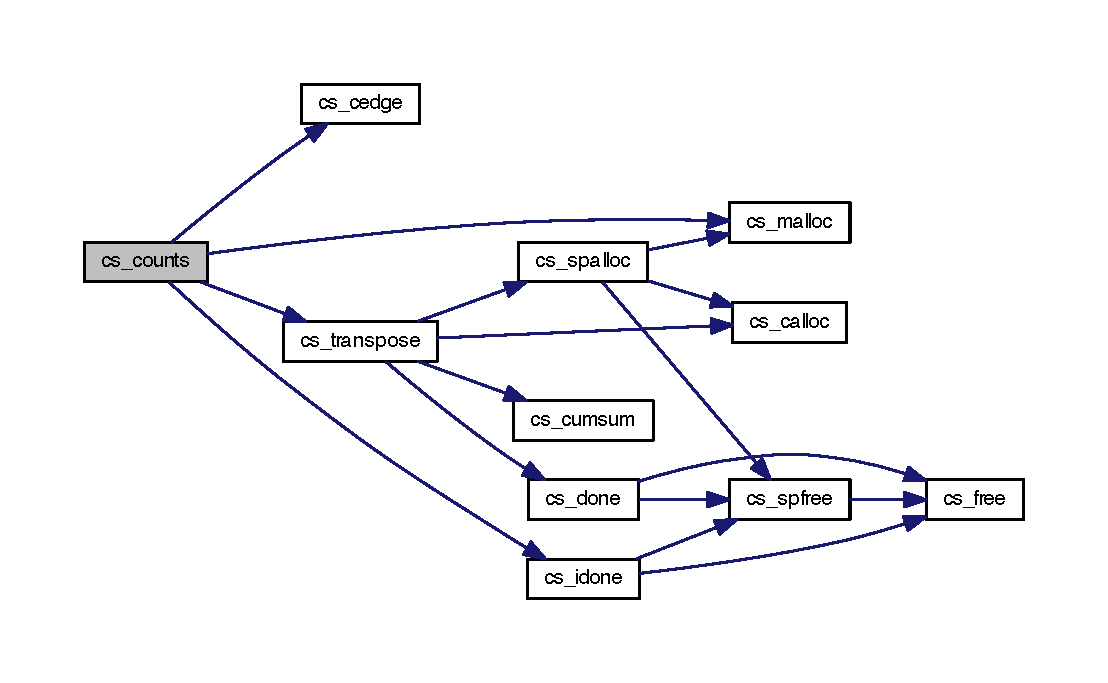
\includegraphics[width=350pt]{csparse_8c_aa7fdeead97aef81cdf18af7576a7f722_cgraph}
\end{center}
\end{figure}


\hypertarget{csparse_8c_afa16a8bc0209e3bd5c0819ed15d2c987}{\index{csparse.\-c@{csparse.\-c}!cs\-\_\-cumsum@{cs\-\_\-cumsum}}
\index{cs\-\_\-cumsum@{cs\-\_\-cumsum}!csparse.c@{csparse.\-c}}
\paragraph[{cs\-\_\-cumsum}]{\setlength{\rightskip}{0pt plus 5cm}int cs\-\_\-cumsum (
\begin{DoxyParamCaption}
\item[{int $\ast$}]{p, }
\item[{int $\ast$}]{c, }
\item[{int}]{n}
\end{DoxyParamCaption}
)}}\label{csparse_8c_afa16a8bc0209e3bd5c0819ed15d2c987}


Definition at line 651 of file csparse.\-c.



Referenced by cs\-\_\-schol(), cs\-\_\-symperm(), cs\-\_\-transpose(), and cs\-\_\-triplet().

\hypertarget{csparse_8c_a30e23f78c9bcbe87e9027d078c98467a}{\index{csparse.\-c@{csparse.\-c}!cs\-\_\-dfs@{cs\-\_\-dfs}}
\index{cs\-\_\-dfs@{cs\-\_\-dfs}!csparse.c@{csparse.\-c}}
\paragraph[{cs\-\_\-dfs}]{\setlength{\rightskip}{0pt plus 5cm}int cs\-\_\-dfs (
\begin{DoxyParamCaption}
\item[{int}]{j, }
\item[{{\bf cs} $\ast$}]{L, }
\item[{int}]{top, }
\item[{int $\ast$}]{xi, }
\item[{int $\ast$}]{pstack, }
\item[{const int $\ast$}]{Pinv}
\end{DoxyParamCaption}
)}}\label{csparse_8c_a30e23f78c9bcbe87e9027d078c98467a}


Definition at line 666 of file csparse.\-c.



References C\-S\-\_\-\-M\-A\-R\-K, C\-S\-\_\-\-M\-A\-R\-K\-E\-D, C\-S\-\_\-\-U\-N\-F\-L\-I\-P, cs\-\_\-sparse\-::i, and cs\-\_\-sparse\-::p.



Referenced by cs\-\_\-reach(), and cs\-\_\-scc().

\hypertarget{csparse_8c_ae296f1a9ad0b70efedc382fae12e028b}{\index{csparse.\-c@{csparse.\-c}!cs\-\_\-bfs@{cs\-\_\-bfs}}
\index{cs\-\_\-bfs@{cs\-\_\-bfs}!csparse.c@{csparse.\-c}}
\paragraph[{cs\-\_\-bfs}]{\setlength{\rightskip}{0pt plus 5cm}static int cs\-\_\-bfs (
\begin{DoxyParamCaption}
\item[{const {\bf cs} $\ast$}]{A, }
\item[{int}]{n, }
\item[{int $\ast$}]{wi, }
\item[{int $\ast$}]{wj, }
\item[{int $\ast$}]{queue, }
\item[{const int $\ast$}]{imatch, }
\item[{const int $\ast$}]{jmatch, }
\item[{int}]{mark}
\end{DoxyParamCaption}
)\hspace{0.3cm}{\ttfamily [static]}}}\label{csparse_8c_ae296f1a9ad0b70efedc382fae12e028b}


Definition at line 703 of file csparse.\-c.



References cs\-\_\-spfree(), cs\-\_\-transpose(), cs\-\_\-sparse\-::i, and cs\-\_\-sparse\-::p.



Referenced by cs\-\_\-dmperm().



Here is the call graph for this function\-:\nopagebreak
\begin{figure}[H]
\begin{center}
\leavevmode
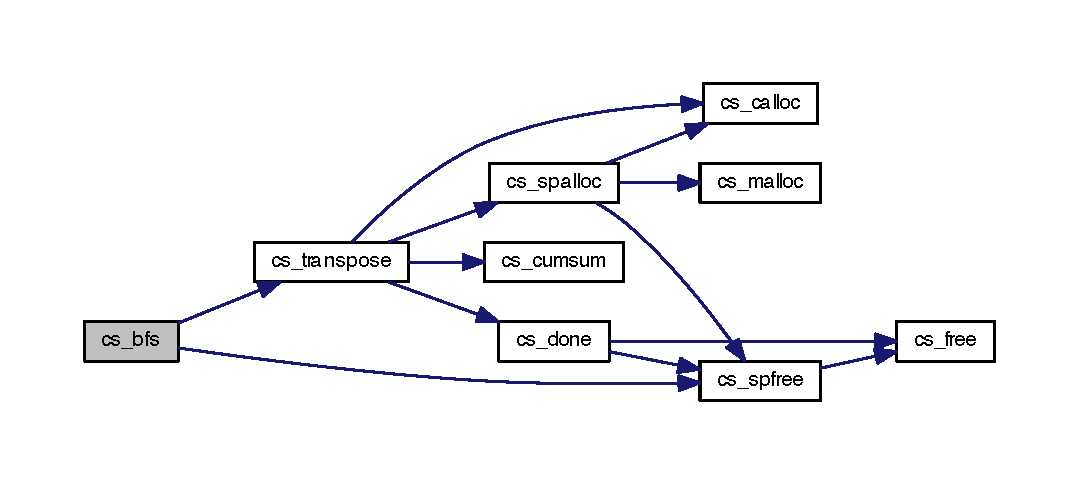
\includegraphics[width=350pt]{csparse_8c_ae296f1a9ad0b70efedc382fae12e028b_cgraph}
\end{center}
\end{figure}


\hypertarget{csparse_8c_a1a8f474b45442c314cadf760871433c3}{\index{csparse.\-c@{csparse.\-c}!cs\-\_\-matched@{cs\-\_\-matched}}
\index{cs\-\_\-matched@{cs\-\_\-matched}!csparse.c@{csparse.\-c}}
\paragraph[{cs\-\_\-matched}]{\setlength{\rightskip}{0pt plus 5cm}static void cs\-\_\-matched (
\begin{DoxyParamCaption}
\item[{int}]{m, }
\item[{const int $\ast$}]{wi, }
\item[{const int $\ast$}]{jmatch, }
\item[{int $\ast$}]{P, }
\item[{int $\ast$}]{Q, }
\item[{int $\ast$}]{cc, }
\item[{int $\ast$}]{rr, }
\item[{int}]{set, }
\item[{int}]{mark}
\end{DoxyParamCaption}
)\hspace{0.3cm}{\ttfamily [static]}}}\label{csparse_8c_a1a8f474b45442c314cadf760871433c3}


Definition at line 738 of file csparse.\-c.



Referenced by cs\-\_\-dmperm().

\hypertarget{csparse_8c_af3bc55de536690597bfefa13d827bcb5}{\index{csparse.\-c@{csparse.\-c}!cs\-\_\-unmatched@{cs\-\_\-unmatched}}
\index{cs\-\_\-unmatched@{cs\-\_\-unmatched}!csparse.c@{csparse.\-c}}
\paragraph[{cs\-\_\-unmatched}]{\setlength{\rightskip}{0pt plus 5cm}static void cs\-\_\-unmatched (
\begin{DoxyParamCaption}
\item[{int}]{m, }
\item[{const int $\ast$}]{wi, }
\item[{int $\ast$}]{P, }
\item[{int $\ast$}]{rr, }
\item[{int}]{set}
\end{DoxyParamCaption}
)\hspace{0.3cm}{\ttfamily [static]}}}\label{csparse_8c_af3bc55de536690597bfefa13d827bcb5}


Definition at line 754 of file csparse.\-c.



Referenced by cs\-\_\-dmperm().

\hypertarget{csparse_8c_ab71ee855eb5dc6e1aa6f0de6a4253d87}{\index{csparse.\-c@{csparse.\-c}!cs\-\_\-rprune@{cs\-\_\-rprune}}
\index{cs\-\_\-rprune@{cs\-\_\-rprune}!csparse.c@{csparse.\-c}}
\paragraph[{cs\-\_\-rprune}]{\setlength{\rightskip}{0pt plus 5cm}static int cs\-\_\-rprune (
\begin{DoxyParamCaption}
\item[{int}]{i, }
\item[{int}]{j, }
\item[{double}]{aij, }
\item[{void $\ast$}]{other}
\end{DoxyParamCaption}
)\hspace{0.3cm}{\ttfamily [static]}}}\label{csparse_8c_ab71ee855eb5dc6e1aa6f0de6a4253d87}


Definition at line 767 of file csparse.\-c.



Referenced by cs\-\_\-dmperm().

\hypertarget{csparse_8c_a59484c944748596c1a9adecfd19085b4}{\index{csparse.\-c@{csparse.\-c}!cs\-\_\-dmperm@{cs\-\_\-dmperm}}
\index{cs\-\_\-dmperm@{cs\-\_\-dmperm}!csparse.c@{csparse.\-c}}
\paragraph[{cs\-\_\-dmperm}]{\setlength{\rightskip}{0pt plus 5cm}{\bf csd}$\ast$ cs\-\_\-dmperm (
\begin{DoxyParamCaption}
\item[{const {\bf cs} $\ast$}]{A}
\end{DoxyParamCaption}
)}}\label{csparse_8c_a59484c944748596c1a9adecfd19085b4}


Definition at line 774 of file csparse.\-c.



References cs\-\_\-dmperm\-\_\-results\-::cc, cs\-\_\-bfs(), cs\-\_\-dalloc(), cs\-\_\-ddone(), cs\-\_\-dfree(), cs\-\_\-fkeep(), cs\-\_\-free(), cs\-\_\-matched(), cs\-\_\-maxtrans(), cs\-\_\-permute(), cs\-\_\-pinv(), cs\-\_\-rprune(), cs\-\_\-scc(), cs\-\_\-unmatched(), cs\-\_\-sparse\-::i, cs\-\_\-sparse\-::m, cs\-\_\-sparse\-::n, cs\-\_\-dmperm\-\_\-results\-::nb, cs\-\_\-sparse\-::p, cs\-\_\-dmperm\-\_\-results\-::\-P, cs\-\_\-dmperm\-\_\-results\-::\-Q, cs\-\_\-dmperm\-\_\-results\-::\-R, cs\-\_\-dmperm\-\_\-results\-::rr, and cs\-\_\-dmperm\-\_\-results\-::\-S.



Here is the call graph for this function\-:\nopagebreak
\begin{figure}[H]
\begin{center}
\leavevmode
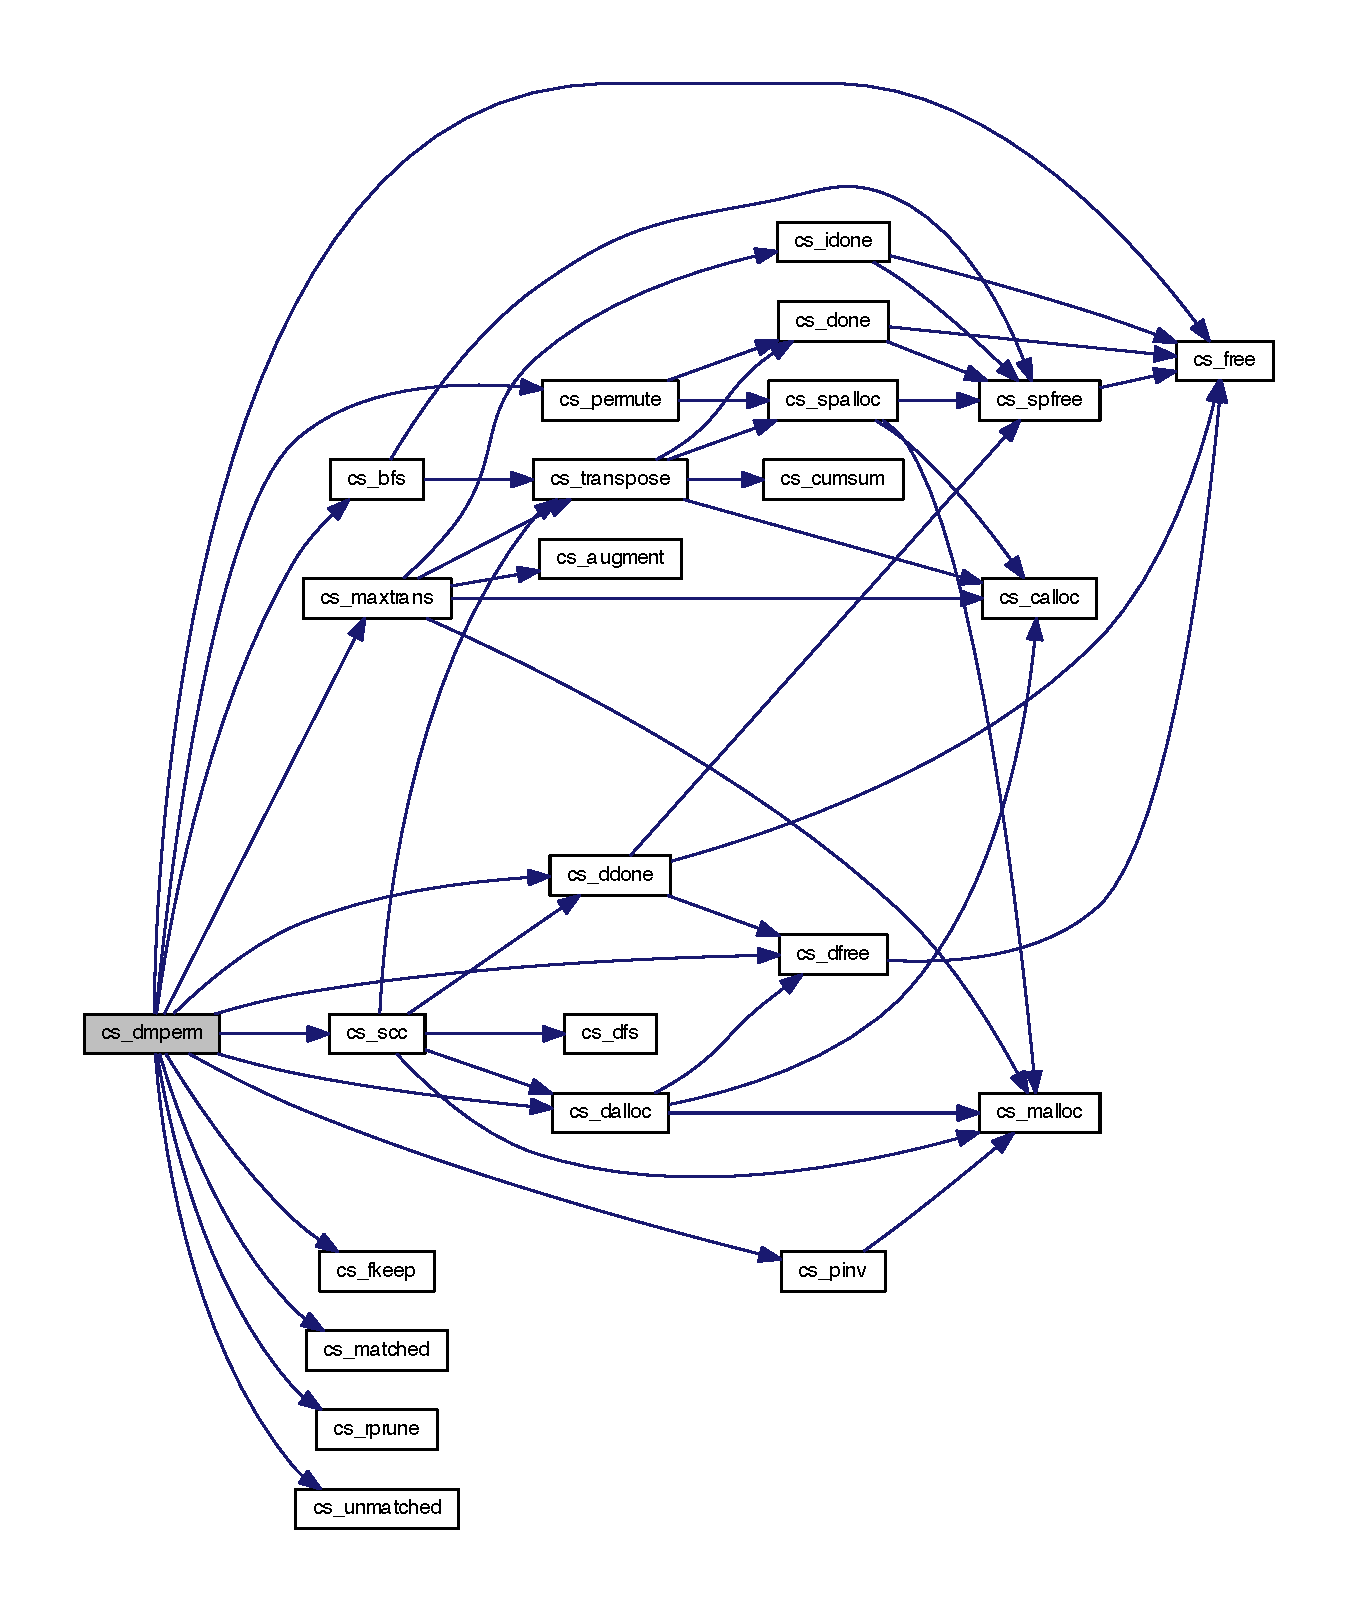
\includegraphics[width=350pt]{csparse_8c_a59484c944748596c1a9adecfd19085b4_cgraph}
\end{center}
\end{figure}


\hypertarget{csparse_8c_adb704422b5f80f757920bf30c5dcabed}{\index{csparse.\-c@{csparse.\-c}!cs\-\_\-tol@{cs\-\_\-tol}}
\index{cs\-\_\-tol@{cs\-\_\-tol}!csparse.c@{csparse.\-c}}
\paragraph[{cs\-\_\-tol}]{\setlength{\rightskip}{0pt plus 5cm}static int cs\-\_\-tol (
\begin{DoxyParamCaption}
\item[{int}]{i, }
\item[{int}]{j, }
\item[{double}]{aij, }
\item[{void $\ast$}]{tol}
\end{DoxyParamCaption}
)\hspace{0.3cm}{\ttfamily [static]}}}\label{csparse_8c_adb704422b5f80f757920bf30c5dcabed}


Definition at line 860 of file csparse.\-c.



Referenced by cs\-\_\-droptol().

\hypertarget{csparse_8c_a39d53ef3034685545cda58ae28af6bb5}{\index{csparse.\-c@{csparse.\-c}!cs\-\_\-droptol@{cs\-\_\-droptol}}
\index{cs\-\_\-droptol@{cs\-\_\-droptol}!csparse.c@{csparse.\-c}}
\paragraph[{cs\-\_\-droptol}]{\setlength{\rightskip}{0pt plus 5cm}int cs\-\_\-droptol (
\begin{DoxyParamCaption}
\item[{{\bf cs} $\ast$}]{A, }
\item[{double}]{tol}
\end{DoxyParamCaption}
)}}\label{csparse_8c_a39d53ef3034685545cda58ae28af6bb5}


Definition at line 864 of file csparse.\-c.



References cs\-\_\-fkeep(), and cs\-\_\-tol().



Here is the call graph for this function\-:\nopagebreak
\begin{figure}[H]
\begin{center}
\leavevmode
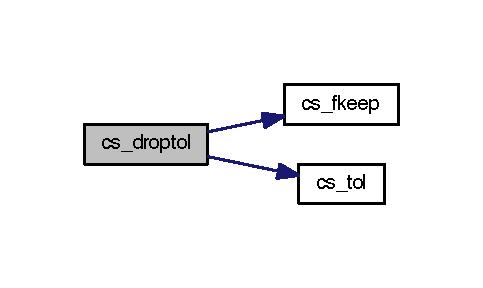
\includegraphics[width=232pt]{csparse_8c_a39d53ef3034685545cda58ae28af6bb5_cgraph}
\end{center}
\end{figure}


\hypertarget{csparse_8c_a9dad9370bdde743eee26de2d53572bda}{\index{csparse.\-c@{csparse.\-c}!cs\-\_\-nonzero@{cs\-\_\-nonzero}}
\index{cs\-\_\-nonzero@{cs\-\_\-nonzero}!csparse.c@{csparse.\-c}}
\paragraph[{cs\-\_\-nonzero}]{\setlength{\rightskip}{0pt plus 5cm}static int cs\-\_\-nonzero (
\begin{DoxyParamCaption}
\item[{int}]{i, }
\item[{int}]{j, }
\item[{double}]{aij, }
\item[{void $\ast$}]{other}
\end{DoxyParamCaption}
)\hspace{0.3cm}{\ttfamily [static]}}}\label{csparse_8c_a9dad9370bdde743eee26de2d53572bda}


Definition at line 869 of file csparse.\-c.



Referenced by cs\-\_\-dropzeros().

\hypertarget{csparse_8c_a50c30e47141ef37dbb4b342e1b4ba924}{\index{csparse.\-c@{csparse.\-c}!cs\-\_\-dropzeros@{cs\-\_\-dropzeros}}
\index{cs\-\_\-dropzeros@{cs\-\_\-dropzeros}!csparse.c@{csparse.\-c}}
\paragraph[{cs\-\_\-dropzeros}]{\setlength{\rightskip}{0pt plus 5cm}int cs\-\_\-dropzeros (
\begin{DoxyParamCaption}
\item[{{\bf cs} $\ast$}]{A}
\end{DoxyParamCaption}
)}}\label{csparse_8c_a50c30e47141ef37dbb4b342e1b4ba924}


Definition at line 873 of file csparse.\-c.



References cs\-\_\-fkeep(), and cs\-\_\-nonzero().



Here is the call graph for this function\-:\nopagebreak
\begin{figure}[H]
\begin{center}
\leavevmode
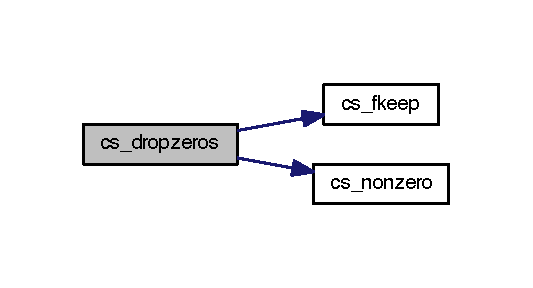
\includegraphics[width=256pt]{csparse_8c_a50c30e47141ef37dbb4b342e1b4ba924_cgraph}
\end{center}
\end{figure}


\hypertarget{csparse_8c_a83dc83954d821b748c3ba9fea1f6b5ca}{\index{csparse.\-c@{csparse.\-c}!cs\-\_\-dupl@{cs\-\_\-dupl}}
\index{cs\-\_\-dupl@{cs\-\_\-dupl}!csparse.c@{csparse.\-c}}
\paragraph[{cs\-\_\-dupl}]{\setlength{\rightskip}{0pt plus 5cm}int cs\-\_\-dupl (
\begin{DoxyParamCaption}
\item[{{\bf cs} $\ast$}]{A}
\end{DoxyParamCaption}
)}}\label{csparse_8c_a83dc83954d821b748c3ba9fea1f6b5ca}


Definition at line 877 of file csparse.\-c.



References cs\-\_\-free(), cs\-\_\-malloc(), cs\-\_\-sprealloc(), cs\-\_\-sparse\-::i, cs\-\_\-sparse\-::m, cs\-\_\-sparse\-::n, cs\-\_\-sparse\-::p, and cs\-\_\-sparse\-::x.



Here is the call graph for this function\-:\nopagebreak
\begin{figure}[H]
\begin{center}
\leavevmode
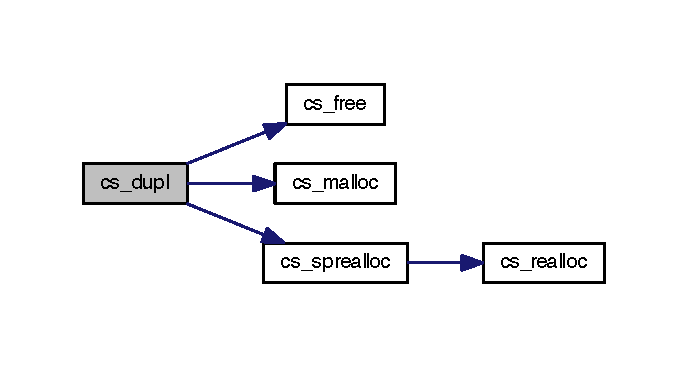
\includegraphics[width=330pt]{csparse_8c_a83dc83954d821b748c3ba9fea1f6b5ca_cgraph}
\end{center}
\end{figure}


\hypertarget{csparse_8c_a123f77ef9b940089a931a994deb21735}{\index{csparse.\-c@{csparse.\-c}!cs\-\_\-entry@{cs\-\_\-entry}}
\index{cs\-\_\-entry@{cs\-\_\-entry}!csparse.c@{csparse.\-c}}
\paragraph[{cs\-\_\-entry}]{\setlength{\rightskip}{0pt plus 5cm}int cs\-\_\-entry (
\begin{DoxyParamCaption}
\item[{{\bf cs} $\ast$}]{T, }
\item[{int}]{i, }
\item[{int}]{j, }
\item[{double}]{x}
\end{DoxyParamCaption}
)}}\label{csparse_8c_a123f77ef9b940089a931a994deb21735}


Definition at line 926 of file csparse.\-c.



References C\-S\-\_\-\-M\-A\-X, cs\-\_\-sprealloc(), cs\-\_\-sparse\-::i, cs\-\_\-sparse\-::m, cs\-\_\-sparse\-::n, cs\-\_\-sparse\-::nz, cs\-\_\-sparse\-::nzmax, cs\-\_\-sparse\-::p, and cs\-\_\-sparse\-::x.



Referenced by cs\-\_\-load().



Here is the call graph for this function\-:\nopagebreak
\begin{figure}[H]
\begin{center}
\leavevmode
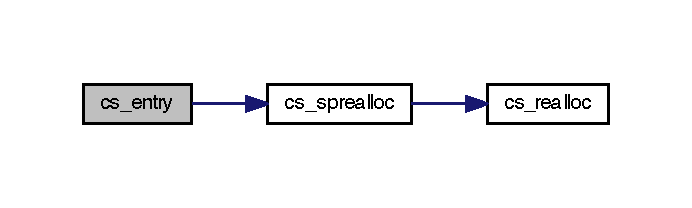
\includegraphics[width=332pt]{csparse_8c_a123f77ef9b940089a931a994deb21735_cgraph}
\end{center}
\end{figure}


\hypertarget{csparse_8c_a5c531804008e67c207e93f14c2551b1a}{\index{csparse.\-c@{csparse.\-c}!cs\-\_\-etree@{cs\-\_\-etree}}
\index{cs\-\_\-etree@{cs\-\_\-etree}!csparse.c@{csparse.\-c}}
\paragraph[{cs\-\_\-etree}]{\setlength{\rightskip}{0pt plus 5cm}int$\ast$ cs\-\_\-etree (
\begin{DoxyParamCaption}
\item[{const {\bf cs} $\ast$}]{A, }
\item[{int}]{ata}
\end{DoxyParamCaption}
)}}\label{csparse_8c_a5c531804008e67c207e93f14c2551b1a}


Definition at line 938 of file csparse.\-c.



References cs\-\_\-idone(), cs\-\_\-malloc(), cs\-\_\-sparse\-::i, cs\-\_\-sparse\-::m, cs\-\_\-sparse\-::n, and cs\-\_\-sparse\-::p.



Referenced by cs\-\_\-schol(), and cs\-\_\-sqr().



Here is the call graph for this function\-:\nopagebreak
\begin{figure}[H]
\begin{center}
\leavevmode
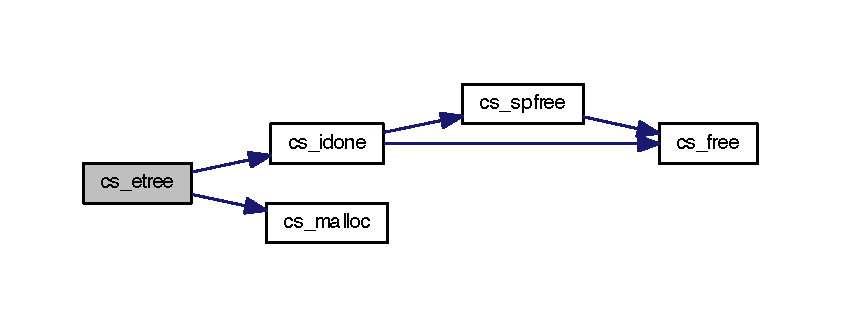
\includegraphics[width=350pt]{csparse_8c_a5c531804008e67c207e93f14c2551b1a_cgraph}
\end{center}
\end{figure}


\hypertarget{csparse_8c_ade63a58ec1758250c64518d817ea3c4c}{\index{csparse.\-c@{csparse.\-c}!cs\-\_\-fkeep@{cs\-\_\-fkeep}}
\index{cs\-\_\-fkeep@{cs\-\_\-fkeep}!csparse.c@{csparse.\-c}}
\paragraph[{cs\-\_\-fkeep}]{\setlength{\rightskip}{0pt plus 5cm}int cs\-\_\-fkeep (
\begin{DoxyParamCaption}
\item[{{\bf cs} $\ast$}]{A, }
\item[{int($\ast$)(int, int, double, void $\ast$)}]{fkeep, }
\item[{void $\ast$}]{other}
\end{DoxyParamCaption}
)}}\label{csparse_8c_ade63a58ec1758250c64518d817ea3c4c}


Definition at line 972 of file csparse.\-c.



References cs\-\_\-sparse\-::i, cs\-\_\-sparse\-::n, cs\-\_\-sparse\-::p, and cs\-\_\-sparse\-::x.



Referenced by cs\-\_\-amd(), cs\-\_\-dmperm(), cs\-\_\-droptol(), and cs\-\_\-dropzeros().

\hypertarget{csparse_8c_a7c887151e9bd6dd56f580c8ae6a5af31}{\index{csparse.\-c@{csparse.\-c}!cs\-\_\-gaxpy@{cs\-\_\-gaxpy}}
\index{cs\-\_\-gaxpy@{cs\-\_\-gaxpy}!csparse.c@{csparse.\-c}}
\paragraph[{cs\-\_\-gaxpy}]{\setlength{\rightskip}{0pt plus 5cm}int cs\-\_\-gaxpy (
\begin{DoxyParamCaption}
\item[{const {\bf cs} $\ast$}]{A, }
\item[{const double $\ast$}]{x, }
\item[{double $\ast$}]{y}
\end{DoxyParamCaption}
)}}\label{csparse_8c_a7c887151e9bd6dd56f580c8ae6a5af31}


Definition at line 998 of file csparse.\-c.



References cs\-\_\-sparse\-::i, cs\-\_\-sparse\-::n, cs\-\_\-sparse\-::p, and cs\-\_\-sparse\-::x.



Referenced by fclib\-\_\-merit\-\_\-local().

\hypertarget{csparse_8c_a27050a31d36046e833b7763fe8ef62ce}{\index{csparse.\-c@{csparse.\-c}!cs\-\_\-happly@{cs\-\_\-happly}}
\index{cs\-\_\-happly@{cs\-\_\-happly}!csparse.c@{csparse.\-c}}
\paragraph[{cs\-\_\-happly}]{\setlength{\rightskip}{0pt plus 5cm}int cs\-\_\-happly (
\begin{DoxyParamCaption}
\item[{const {\bf cs} $\ast$}]{V, }
\item[{int}]{i, }
\item[{double}]{beta, }
\item[{double $\ast$}]{x}
\end{DoxyParamCaption}
)}}\label{csparse_8c_a27050a31d36046e833b7763fe8ef62ce}


Definition at line 1018 of file csparse.\-c.



References cs\-\_\-sparse\-::i, cs\-\_\-sparse\-::p, and cs\-\_\-sparse\-::x.



Referenced by cs\-\_\-qr(), and cs\-\_\-qrsol().

\hypertarget{csparse_8c_a096c9057bf2038f9eaef0c1dfb09f3dd}{\index{csparse.\-c@{csparse.\-c}!cs\-\_\-house@{cs\-\_\-house}}
\index{cs\-\_\-house@{cs\-\_\-house}!csparse.c@{csparse.\-c}}
\paragraph[{cs\-\_\-house}]{\setlength{\rightskip}{0pt plus 5cm}double cs\-\_\-house (
\begin{DoxyParamCaption}
\item[{double $\ast$}]{x, }
\item[{double $\ast$}]{beta, }
\item[{int}]{n}
\end{DoxyParamCaption}
)}}\label{csparse_8c_a096c9057bf2038f9eaef0c1dfb09f3dd}


Definition at line 1040 of file csparse.\-c.



Referenced by cs\-\_\-qr().

\hypertarget{csparse_8c_a51a8d1a79477ff438a978ab1d8f9849b}{\index{csparse.\-c@{csparse.\-c}!cs\-\_\-ipvec@{cs\-\_\-ipvec}}
\index{cs\-\_\-ipvec@{cs\-\_\-ipvec}!csparse.c@{csparse.\-c}}
\paragraph[{cs\-\_\-ipvec}]{\setlength{\rightskip}{0pt plus 5cm}int cs\-\_\-ipvec (
\begin{DoxyParamCaption}
\item[{int}]{n, }
\item[{const int $\ast$}]{P, }
\item[{const double $\ast$}]{b, }
\item[{double $\ast$}]{x}
\end{DoxyParamCaption}
)}}\label{csparse_8c_a51a8d1a79477ff438a978ab1d8f9849b}


Definition at line 1062 of file csparse.\-c.



Referenced by cs\-\_\-cholsol(), cs\-\_\-lusol(), and cs\-\_\-qrsol().

\hypertarget{csparse_8c_a12eb66c4f53e51ee5e03ec0b9f24b368}{\index{csparse.\-c@{csparse.\-c}!cs\-\_\-load@{cs\-\_\-load}}
\index{cs\-\_\-load@{cs\-\_\-load}!csparse.c@{csparse.\-c}}
\paragraph[{cs\-\_\-load}]{\setlength{\rightskip}{0pt plus 5cm}{\bf cs}$\ast$ cs\-\_\-load (
\begin{DoxyParamCaption}
\item[{F\-I\-L\-E $\ast$}]{f}
\end{DoxyParamCaption}
)}}\label{csparse_8c_a12eb66c4f53e51ee5e03ec0b9f24b368}


Definition at line 1069 of file csparse.\-c.



References cs\-\_\-entry(), cs\-\_\-spalloc(), and cs\-\_\-spfree().



Here is the call graph for this function\-:\nopagebreak
\begin{figure}[H]
\begin{center}
\leavevmode
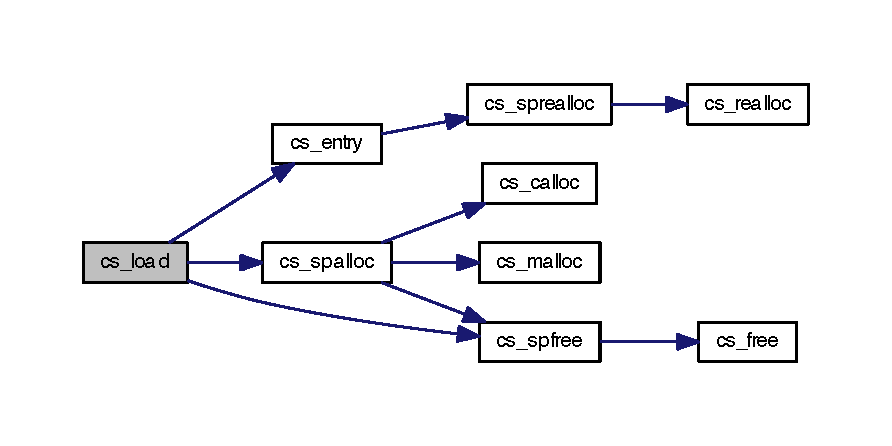
\includegraphics[width=350pt]{csparse_8c_a12eb66c4f53e51ee5e03ec0b9f24b368_cgraph}
\end{center}
\end{figure}


\hypertarget{csparse_8c_adbd011bdb4d7bef9825ca1c743fc6b46}{\index{csparse.\-c@{csparse.\-c}!cs\-\_\-lsolve@{cs\-\_\-lsolve}}
\index{cs\-\_\-lsolve@{cs\-\_\-lsolve}!csparse.c@{csparse.\-c}}
\paragraph[{cs\-\_\-lsolve}]{\setlength{\rightskip}{0pt plus 5cm}int cs\-\_\-lsolve (
\begin{DoxyParamCaption}
\item[{const {\bf cs} $\ast$}]{L, }
\item[{double $\ast$}]{x}
\end{DoxyParamCaption}
)}}\label{csparse_8c_adbd011bdb4d7bef9825ca1c743fc6b46}


Definition at line 1093 of file csparse.\-c.



References cs\-\_\-sparse\-::i, cs\-\_\-sparse\-::n, cs\-\_\-sparse\-::p, and cs\-\_\-sparse\-::x.



Referenced by cs\-\_\-cholsol(), and cs\-\_\-lusol().

\hypertarget{csparse_8c_afc61741ee2f33a3544f1c5f6b9caf9f6}{\index{csparse.\-c@{csparse.\-c}!cs\-\_\-ltsolve@{cs\-\_\-ltsolve}}
\index{cs\-\_\-ltsolve@{cs\-\_\-ltsolve}!csparse.c@{csparse.\-c}}
\paragraph[{cs\-\_\-ltsolve}]{\setlength{\rightskip}{0pt plus 5cm}int cs\-\_\-ltsolve (
\begin{DoxyParamCaption}
\item[{const {\bf cs} $\ast$}]{L, }
\item[{double $\ast$}]{x}
\end{DoxyParamCaption}
)}}\label{csparse_8c_afc61741ee2f33a3544f1c5f6b9caf9f6}


Definition at line 1127 of file csparse.\-c.



References cs\-\_\-sparse\-::i, cs\-\_\-sparse\-::n, cs\-\_\-sparse\-::p, and cs\-\_\-sparse\-::x.



Referenced by cs\-\_\-cholsol().

\hypertarget{csparse_8c_a6a35ad4816f210234a33eed09b19d181}{\index{csparse.\-c@{csparse.\-c}!cs\-\_\-lu@{cs\-\_\-lu}}
\index{cs\-\_\-lu@{cs\-\_\-lu}!csparse.c@{csparse.\-c}}
\paragraph[{cs\-\_\-lu}]{\setlength{\rightskip}{0pt plus 5cm}{\bf csn}$\ast$ cs\-\_\-lu (
\begin{DoxyParamCaption}
\item[{const {\bf cs} $\ast$}]{A, }
\item[{const {\bf css} $\ast$}]{S, }
\item[{double}]{tol}
\end{DoxyParamCaption}
)}}\label{csparse_8c_a6a35ad4816f210234a33eed09b19d181}


Definition at line 1163 of file csparse.\-c.



References cs\-\_\-calloc(), cs\-\_\-malloc(), cs\-\_\-ndone(), cs\-\_\-spalloc(), cs\-\_\-splsolve(), cs\-\_\-sprealloc(), cs\-\_\-sparse\-::i, cs\-\_\-numeric\-::\-L, cs\-\_\-symbolic\-::lnz, cs\-\_\-sparse\-::n, cs\-\_\-sparse\-::nzmax, cs\-\_\-sparse\-::p, cs\-\_\-numeric\-::\-Pinv, cs\-\_\-symbolic\-::\-Q, cs\-\_\-numeric\-::\-U, cs\-\_\-symbolic\-::unz, and cs\-\_\-sparse\-::x.



Referenced by cs\-\_\-lusol().



Here is the call graph for this function\-:\nopagebreak
\begin{figure}[H]
\begin{center}
\leavevmode
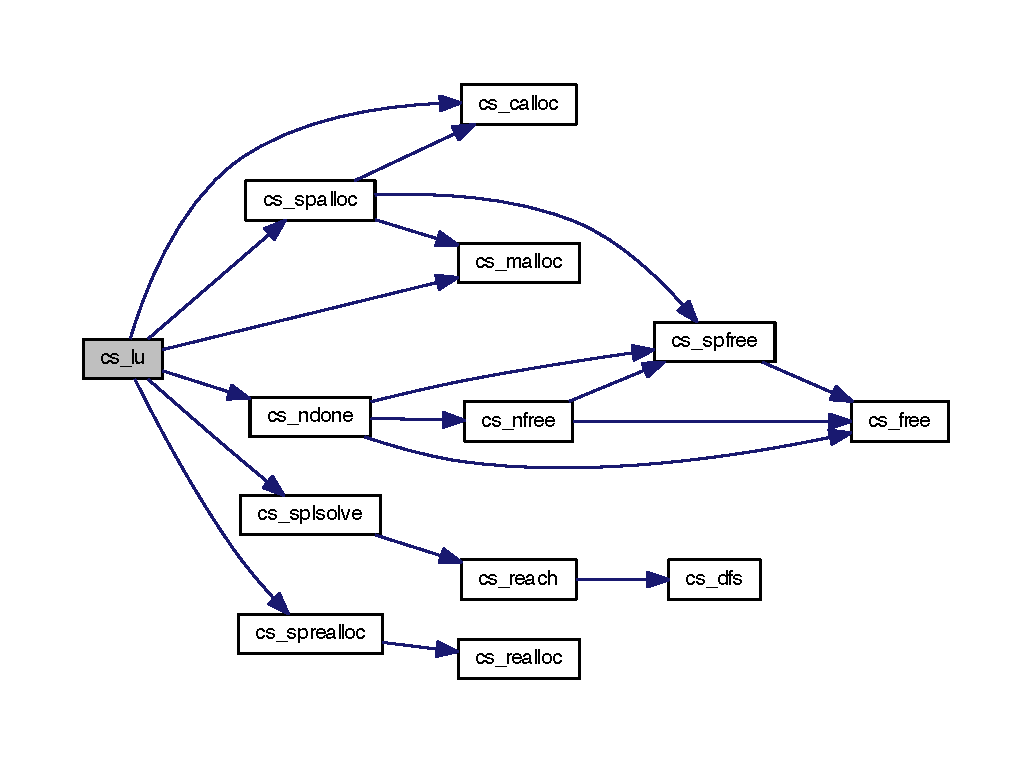
\includegraphics[width=350pt]{csparse_8c_a6a35ad4816f210234a33eed09b19d181_cgraph}
\end{center}
\end{figure}


\hypertarget{csparse_8c_a14612df0010f5284c8f3feac2a7e02fd}{\index{csparse.\-c@{csparse.\-c}!cs\-\_\-lusol@{cs\-\_\-lusol}}
\index{cs\-\_\-lusol@{cs\-\_\-lusol}!csparse.c@{csparse.\-c}}
\paragraph[{cs\-\_\-lusol}]{\setlength{\rightskip}{0pt plus 5cm}int cs\-\_\-lusol (
\begin{DoxyParamCaption}
\item[{const {\bf cs} $\ast$}]{A, }
\item[{double $\ast$}]{b, }
\item[{int}]{order, }
\item[{double}]{tol}
\end{DoxyParamCaption}
)}}\label{csparse_8c_a14612df0010f5284c8f3feac2a7e02fd}


Definition at line 1255 of file csparse.\-c.



References cs\-\_\-free(), cs\-\_\-ipvec(), cs\-\_\-lsolve(), cs\-\_\-lu(), cs\-\_\-malloc(), cs\-\_\-nfree(), cs\-\_\-sfree(), cs\-\_\-sqr(), cs\-\_\-usolve(), cs\-\_\-numeric\-::\-L, cs\-\_\-sparse\-::n, cs\-\_\-numeric\-::\-Pinv, cs\-\_\-symbolic\-::\-Q, and cs\-\_\-numeric\-::\-U.



Here is the call graph for this function\-:\nopagebreak
\begin{figure}[H]
\begin{center}
\leavevmode
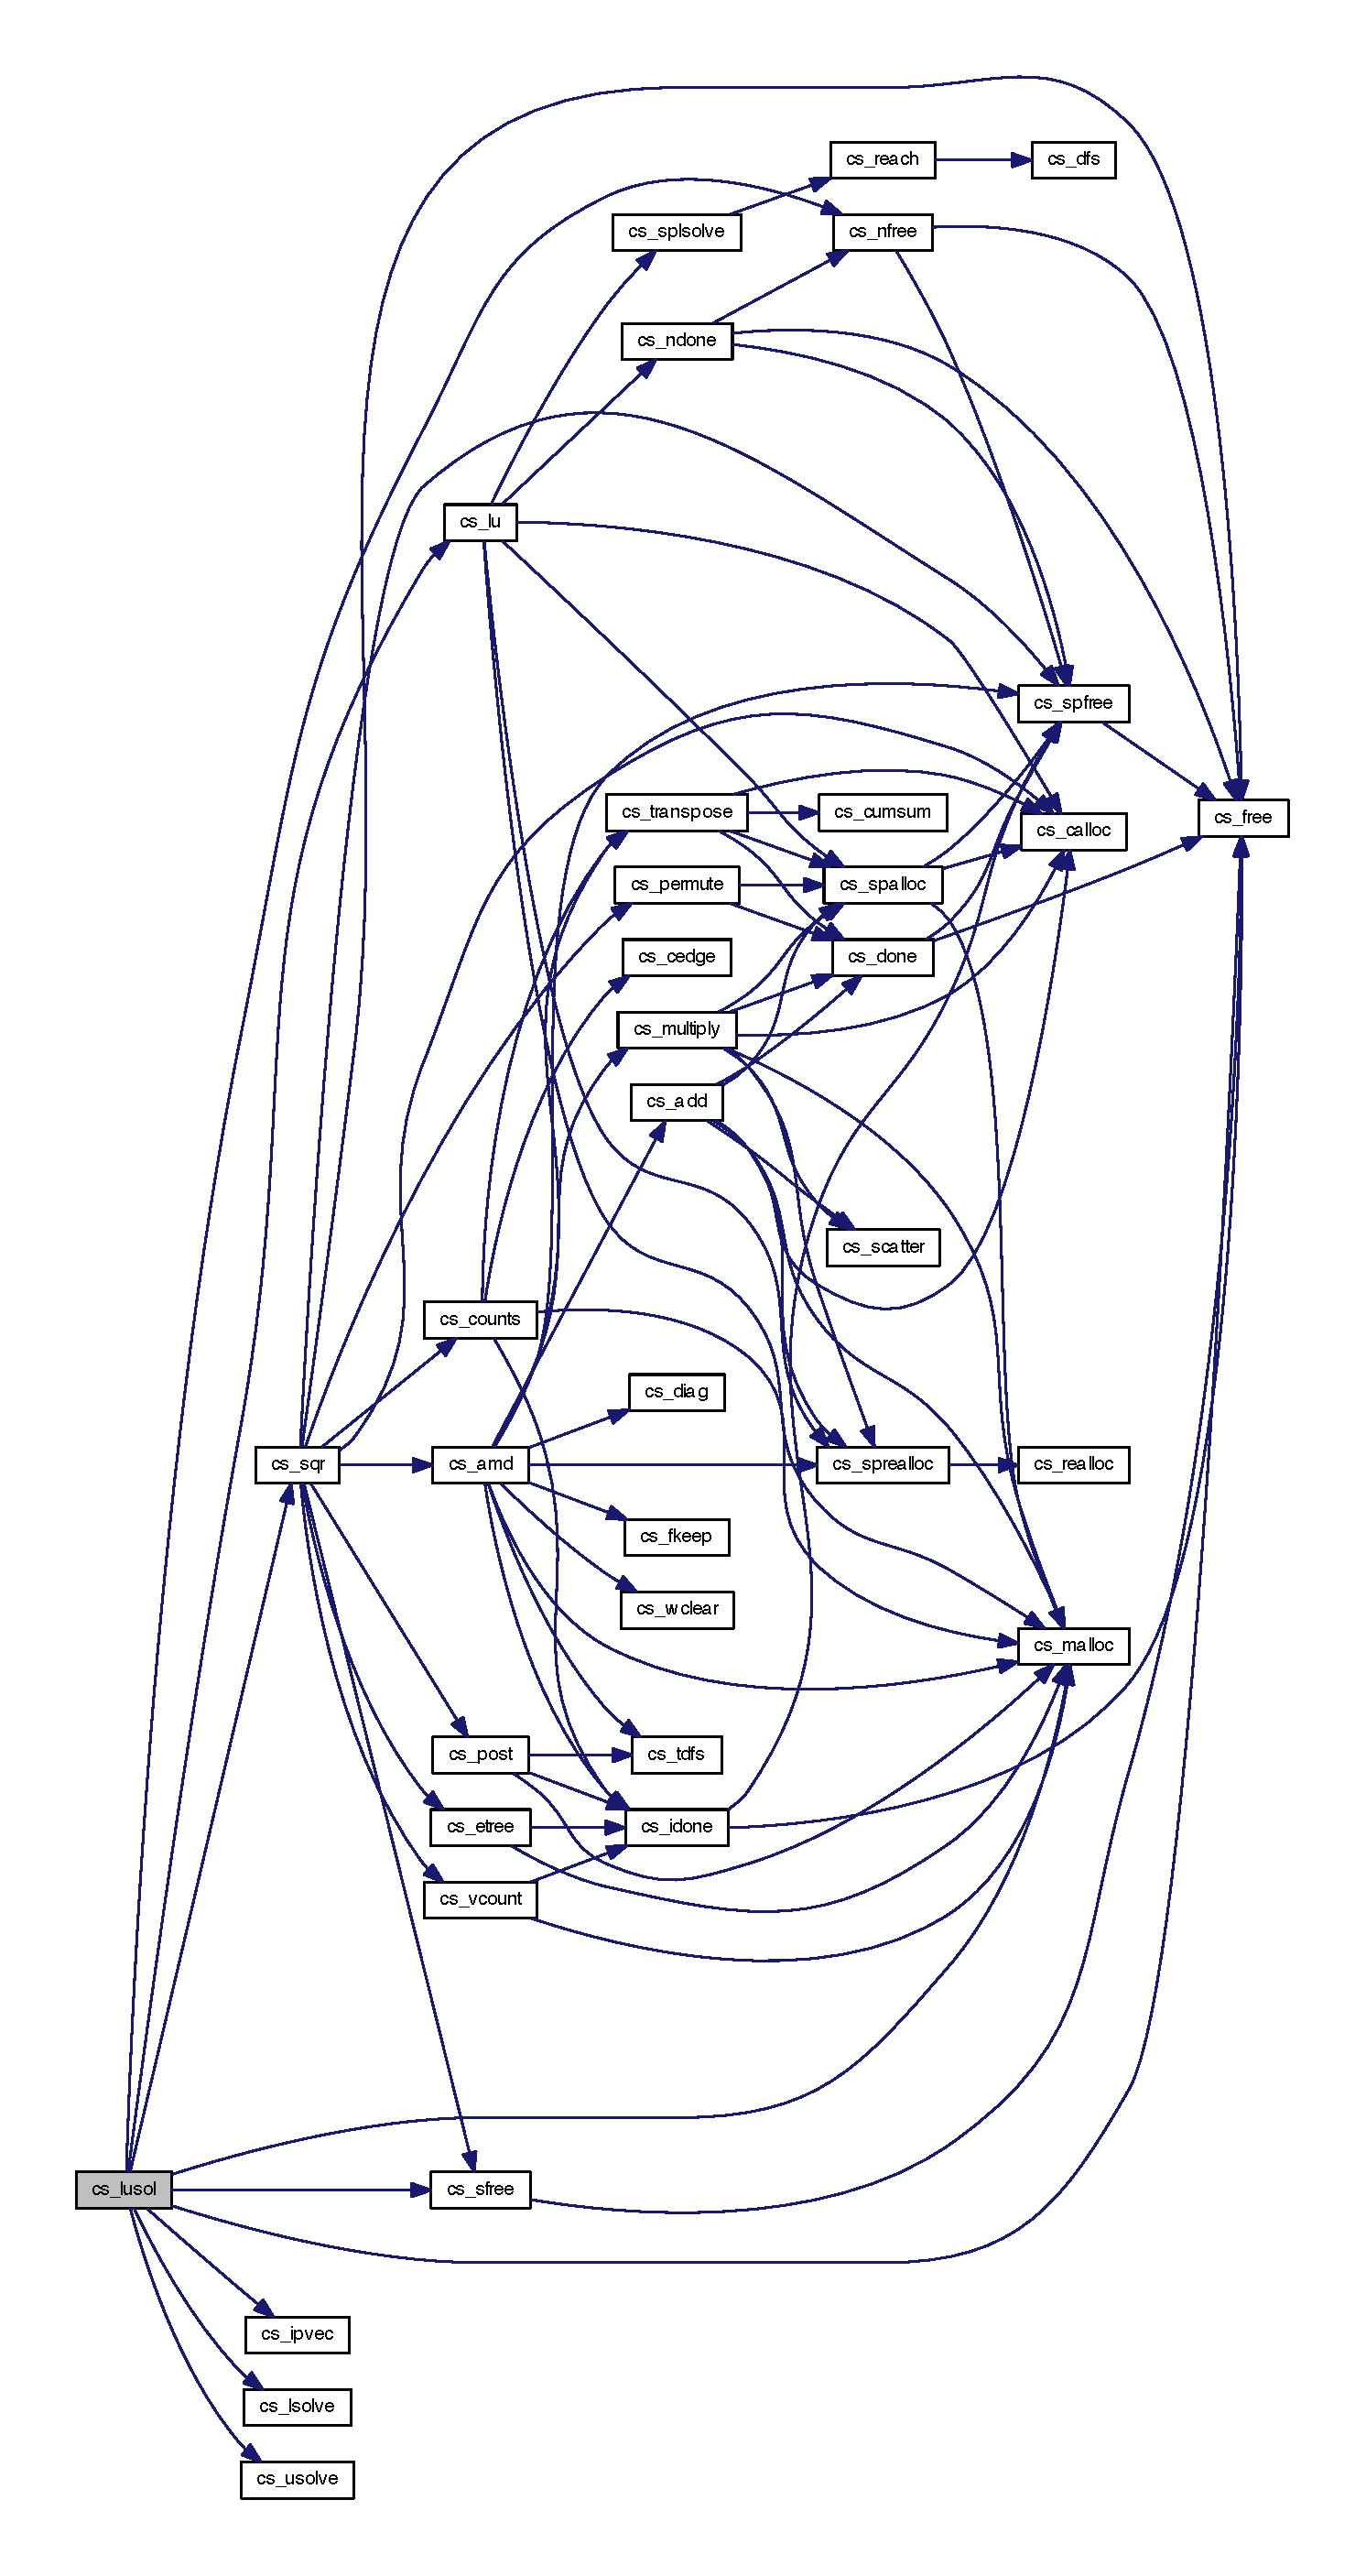
\includegraphics[height=550pt]{csparse_8c_a14612df0010f5284c8f3feac2a7e02fd_cgraph}
\end{center}
\end{figure}


\hypertarget{csparse_8c_a4c6c75c54cbdf2f3fd4574a90c2f8a86}{\index{csparse.\-c@{csparse.\-c}!cs\-\_\-malloc@{cs\-\_\-malloc}}
\index{cs\-\_\-malloc@{cs\-\_\-malloc}!csparse.c@{csparse.\-c}}
\paragraph[{cs\-\_\-malloc}]{\setlength{\rightskip}{0pt plus 5cm}void$\ast$ cs\-\_\-malloc (
\begin{DoxyParamCaption}
\item[{int}]{n, }
\item[{size\-\_\-t}]{size}
\end{DoxyParamCaption}
)}}\label{csparse_8c_a4c6c75c54cbdf2f3fd4574a90c2f8a86}


Definition at line 1288 of file csparse.\-c.



References C\-S\-\_\-\-M\-A\-X, and C\-S\-\_\-\-O\-V\-E\-R\-F\-L\-O\-W.



Referenced by cs\-\_\-add(), cs\-\_\-amd(), cs\-\_\-chol(), cs\-\_\-cholsol(), cs\-\_\-counts(), cs\-\_\-dalloc(), cs\-\_\-dupl(), cs\-\_\-etree(), cs\-\_\-lu(), cs\-\_\-lusol(), cs\-\_\-maxtrans(), cs\-\_\-multiply(), cs\-\_\-pinv(), cs\-\_\-post(), cs\-\_\-qr(), cs\-\_\-scc(), cs\-\_\-schol(), cs\-\_\-spalloc(), cs\-\_\-updown(), and cs\-\_\-vcount().

\hypertarget{csparse_8c_ad3e846c0142a1457e8e85bcaf559fb98}{\index{csparse.\-c@{csparse.\-c}!cs\-\_\-calloc@{cs\-\_\-calloc}}
\index{cs\-\_\-calloc@{cs\-\_\-calloc}!csparse.c@{csparse.\-c}}
\paragraph[{cs\-\_\-calloc}]{\setlength{\rightskip}{0pt plus 5cm}void$\ast$ cs\-\_\-calloc (
\begin{DoxyParamCaption}
\item[{int}]{n, }
\item[{size\-\_\-t}]{size}
\end{DoxyParamCaption}
)}}\label{csparse_8c_ad3e846c0142a1457e8e85bcaf559fb98}


Definition at line 1294 of file csparse.\-c.



References C\-S\-\_\-\-M\-A\-X, and C\-S\-\_\-\-O\-V\-E\-R\-F\-L\-O\-W.



Referenced by cs\-\_\-add(), cs\-\_\-chol(), cs\-\_\-dalloc(), cs\-\_\-lu(), cs\-\_\-maxtrans(), cs\-\_\-multiply(), cs\-\_\-qr(), cs\-\_\-qrsol(), cs\-\_\-schol(), cs\-\_\-spalloc(), cs\-\_\-sqr(), cs\-\_\-symperm(), cs\-\_\-transpose(), and cs\-\_\-triplet().

\hypertarget{csparse_8c_a78c1d1194aacc65212bb0d2b03643ac7}{\index{csparse.\-c@{csparse.\-c}!cs\-\_\-free@{cs\-\_\-free}}
\index{cs\-\_\-free@{cs\-\_\-free}!csparse.c@{csparse.\-c}}
\paragraph[{cs\-\_\-free}]{\setlength{\rightskip}{0pt plus 5cm}void$\ast$ cs\-\_\-free (
\begin{DoxyParamCaption}
\item[{void $\ast$}]{p}
\end{DoxyParamCaption}
)}}\label{csparse_8c_a78c1d1194aacc65212bb0d2b03643ac7}


Definition at line 1300 of file csparse.\-c.



Referenced by cs\-\_\-cholsol(), cs\-\_\-ddone(), cs\-\_\-dfree(), cs\-\_\-dmperm(), cs\-\_\-done(), cs\-\_\-dupl(), cs\-\_\-idone(), cs\-\_\-lusol(), cs\-\_\-ndone(), cs\-\_\-nfree(), cs\-\_\-qrsol(), cs\-\_\-schol(), cs\-\_\-sfree(), cs\-\_\-spfree(), cs\-\_\-sqr(), and cs\-\_\-updown().

\hypertarget{csparse_8c_a7e829e1175f2c8ddb0d6d9e0bb90f985}{\index{csparse.\-c@{csparse.\-c}!cs\-\_\-realloc@{cs\-\_\-realloc}}
\index{cs\-\_\-realloc@{cs\-\_\-realloc}!csparse.c@{csparse.\-c}}
\paragraph[{cs\-\_\-realloc}]{\setlength{\rightskip}{0pt plus 5cm}void$\ast$ cs\-\_\-realloc (
\begin{DoxyParamCaption}
\item[{void $\ast$}]{p, }
\item[{int}]{n, }
\item[{size\-\_\-t}]{size, }
\item[{int $\ast$}]{ok}
\end{DoxyParamCaption}
)}}\label{csparse_8c_a7e829e1175f2c8ddb0d6d9e0bb90f985}


Definition at line 1307 of file csparse.\-c.



References C\-S\-\_\-\-M\-A\-X, and C\-S\-\_\-\-O\-V\-E\-R\-F\-L\-O\-W.



Referenced by cs\-\_\-sprealloc().

\hypertarget{csparse_8c_a76ac84cfd998800844b585a556a5f6ad}{\index{csparse.\-c@{csparse.\-c}!cs\-\_\-augment@{cs\-\_\-augment}}
\index{cs\-\_\-augment@{cs\-\_\-augment}!csparse.c@{csparse.\-c}}
\paragraph[{cs\-\_\-augment}]{\setlength{\rightskip}{0pt plus 5cm}static void cs\-\_\-augment (
\begin{DoxyParamCaption}
\item[{int}]{k, }
\item[{const {\bf cs} $\ast$}]{A, }
\item[{int $\ast$}]{jmatch, }
\item[{int $\ast$}]{cheap, }
\item[{int $\ast$}]{w, }
\item[{int $\ast$}]{js, }
\item[{int $\ast$}]{is, }
\item[{int $\ast$}]{ps}
\end{DoxyParamCaption}
)\hspace{0.3cm}{\ttfamily [static]}}}\label{csparse_8c_a76ac84cfd998800844b585a556a5f6ad}


Definition at line 1318 of file csparse.\-c.



References cs\-\_\-sparse\-::i, and cs\-\_\-sparse\-::p.



Referenced by cs\-\_\-maxtrans().

\hypertarget{csparse_8c_aebd7035aaa1627313149c32755b9f642}{\index{csparse.\-c@{csparse.\-c}!cs\-\_\-maxtrans@{cs\-\_\-maxtrans}}
\index{cs\-\_\-maxtrans@{cs\-\_\-maxtrans}!csparse.c@{csparse.\-c}}
\paragraph[{cs\-\_\-maxtrans}]{\setlength{\rightskip}{0pt plus 5cm}int$\ast$ cs\-\_\-maxtrans (
\begin{DoxyParamCaption}
\item[{const {\bf cs} $\ast$}]{A}
\end{DoxyParamCaption}
)}}\label{csparse_8c_aebd7035aaa1627313149c32755b9f642}


Definition at line 1359 of file csparse.\-c.



References cs\-\_\-augment(), cs\-\_\-calloc(), cs\-\_\-idone(), cs\-\_\-malloc(), cs\-\_\-transpose(), cs\-\_\-sparse\-::i, cs\-\_\-sparse\-::m, cs\-\_\-sparse\-::n, and cs\-\_\-sparse\-::p.



Referenced by cs\-\_\-dmperm().



Here is the call graph for this function\-:\nopagebreak
\begin{figure}[H]
\begin{center}
\leavevmode
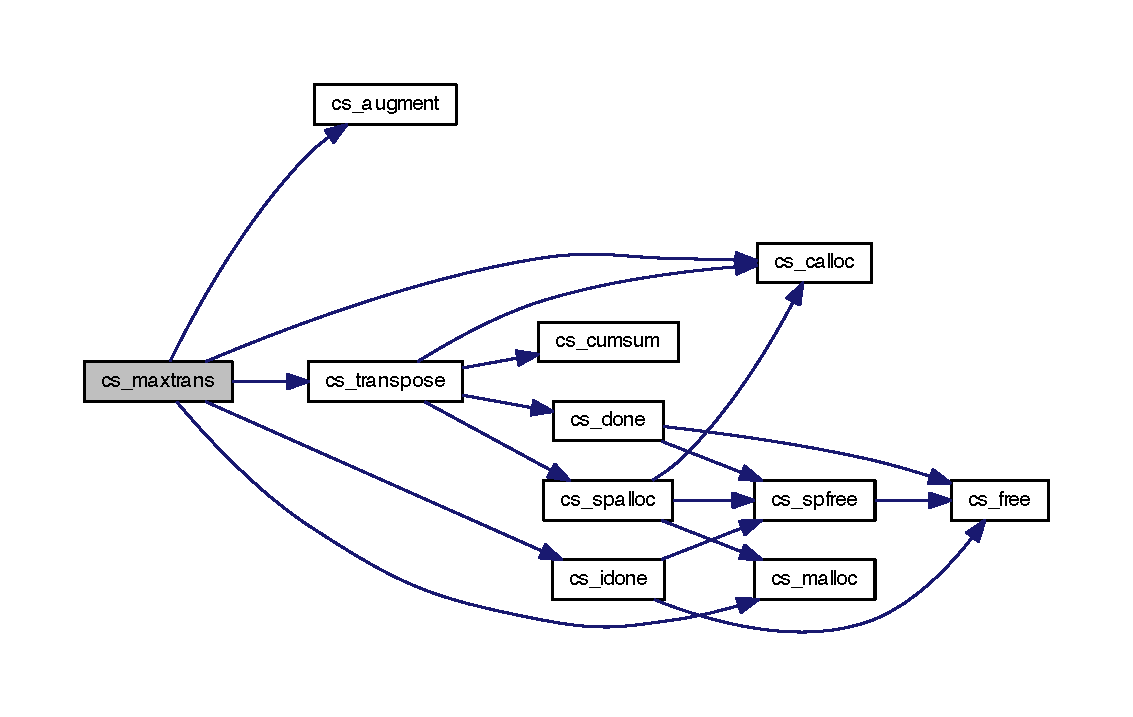
\includegraphics[width=350pt]{csparse_8c_aebd7035aaa1627313149c32755b9f642_cgraph}
\end{center}
\end{figure}


\hypertarget{csparse_8c_a066e18f8570c820530c73ebc88b30a97}{\index{csparse.\-c@{csparse.\-c}!cs\-\_\-multiply@{cs\-\_\-multiply}}
\index{cs\-\_\-multiply@{cs\-\_\-multiply}!csparse.c@{csparse.\-c}}
\paragraph[{cs\-\_\-multiply}]{\setlength{\rightskip}{0pt plus 5cm}{\bf cs}$\ast$ cs\-\_\-multiply (
\begin{DoxyParamCaption}
\item[{const {\bf cs} $\ast$}]{A, }
\item[{const {\bf cs} $\ast$}]{B}
\end{DoxyParamCaption}
)}}\label{csparse_8c_a066e18f8570c820530c73ebc88b30a97}


Definition at line 1400 of file csparse.\-c.



References cs\-\_\-calloc(), cs\-\_\-done(), cs\-\_\-malloc(), cs\-\_\-scatter(), cs\-\_\-spalloc(), cs\-\_\-sprealloc(), cs\-\_\-sparse\-::i, cs\-\_\-sparse\-::m, cs\-\_\-sparse\-::n, cs\-\_\-sparse\-::p, and cs\-\_\-sparse\-::x.



Referenced by cs\-\_\-amd().



Here is the call graph for this function\-:\nopagebreak
\begin{figure}[H]
\begin{center}
\leavevmode
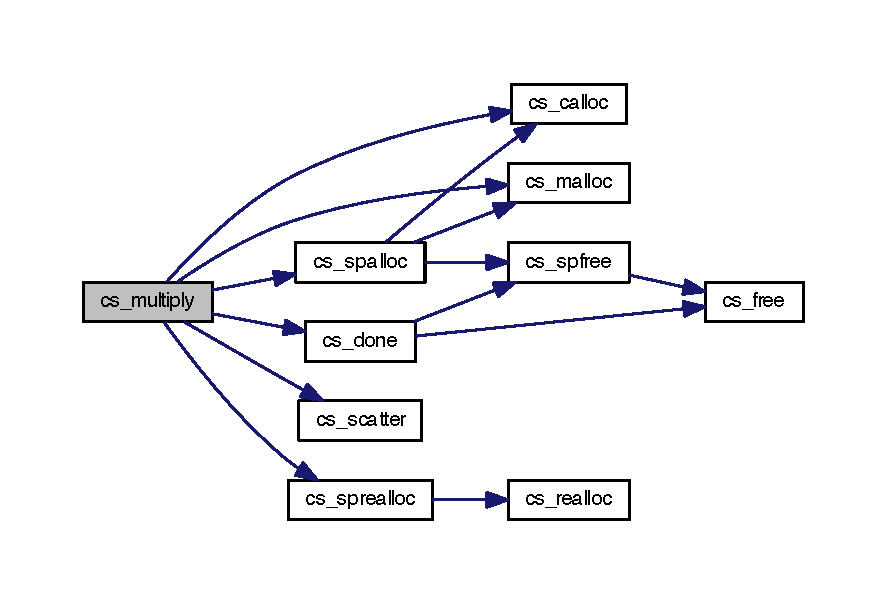
\includegraphics[width=350pt]{csparse_8c_a066e18f8570c820530c73ebc88b30a97_cgraph}
\end{center}
\end{figure}


\hypertarget{csparse_8c_ae2b324f8f0cdc3610d98ce6cebd50075}{\index{csparse.\-c@{csparse.\-c}!cs\-\_\-norm@{cs\-\_\-norm}}
\index{cs\-\_\-norm@{cs\-\_\-norm}!csparse.c@{csparse.\-c}}
\paragraph[{cs\-\_\-norm}]{\setlength{\rightskip}{0pt plus 5cm}double cs\-\_\-norm (
\begin{DoxyParamCaption}
\item[{const {\bf cs} $\ast$}]{A}
\end{DoxyParamCaption}
)}}\label{csparse_8c_ae2b324f8f0cdc3610d98ce6cebd50075}


Definition at line 1440 of file csparse.\-c.



References C\-S\-\_\-\-M\-A\-X, cs\-\_\-sparse\-::n, cs\-\_\-sparse\-::p, and cs\-\_\-sparse\-::x.



Referenced by cs\-\_\-print().

\hypertarget{csparse_8c_a752362fe7bf8d0d49d3c2d788f4d38a9}{\index{csparse.\-c@{csparse.\-c}!cs\-\_\-permute@{cs\-\_\-permute}}
\index{cs\-\_\-permute@{cs\-\_\-permute}!csparse.c@{csparse.\-c}}
\paragraph[{cs\-\_\-permute}]{\setlength{\rightskip}{0pt plus 5cm}{\bf cs}$\ast$ cs\-\_\-permute (
\begin{DoxyParamCaption}
\item[{const {\bf cs} $\ast$}]{A, }
\item[{const int $\ast$}]{Pinv, }
\item[{const int $\ast$}]{Q, }
\item[{int}]{values}
\end{DoxyParamCaption}
)}}\label{csparse_8c_a752362fe7bf8d0d49d3c2d788f4d38a9}


Definition at line 1457 of file csparse.\-c.



References cs\-\_\-done(), cs\-\_\-spalloc(), cs\-\_\-sparse\-::i, cs\-\_\-sparse\-::m, cs\-\_\-sparse\-::n, cs\-\_\-sparse\-::p, and cs\-\_\-sparse\-::x.



Referenced by cs\-\_\-dmperm(), and cs\-\_\-sqr().



Here is the call graph for this function\-:\nopagebreak
\begin{figure}[H]
\begin{center}
\leavevmode
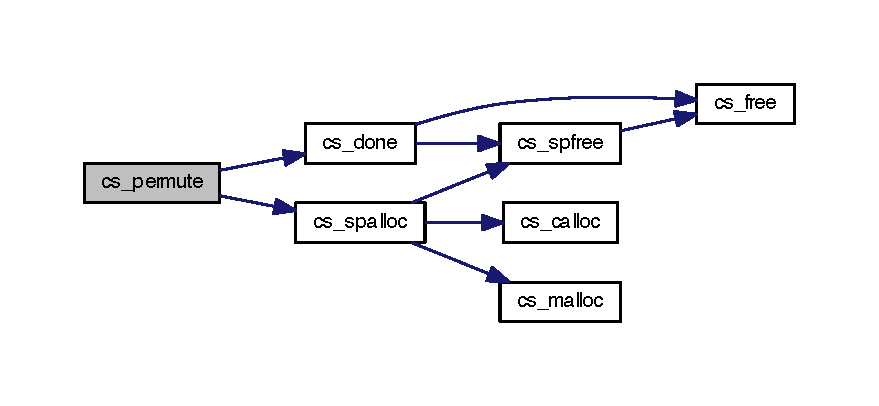
\includegraphics[width=350pt]{csparse_8c_a752362fe7bf8d0d49d3c2d788f4d38a9_cgraph}
\end{center}
\end{figure}


\hypertarget{csparse_8c_af29c4a6ca5cea4b9ffa1cbf24636bbc6}{\index{csparse.\-c@{csparse.\-c}!cs\-\_\-pinv@{cs\-\_\-pinv}}
\index{cs\-\_\-pinv@{cs\-\_\-pinv}!csparse.c@{csparse.\-c}}
\paragraph[{cs\-\_\-pinv}]{\setlength{\rightskip}{0pt plus 5cm}int$\ast$ cs\-\_\-pinv (
\begin{DoxyParamCaption}
\item[{int const $\ast$}]{P, }
\item[{int}]{n}
\end{DoxyParamCaption}
)}}\label{csparse_8c_af29c4a6ca5cea4b9ffa1cbf24636bbc6}


Definition at line 1488 of file csparse.\-c.



References cs\-\_\-malloc().



Referenced by cs\-\_\-dmperm(), and cs\-\_\-schol().



Here is the call graph for this function\-:\nopagebreak
\begin{figure}[H]
\begin{center}
\leavevmode
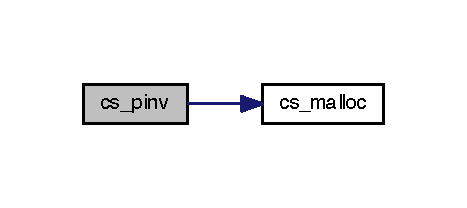
\includegraphics[width=224pt]{csparse_8c_af29c4a6ca5cea4b9ffa1cbf24636bbc6_cgraph}
\end{center}
\end{figure}


\hypertarget{csparse_8c_af84bc0a35c099a9a1e01e5aebf8c7292}{\index{csparse.\-c@{csparse.\-c}!cs\-\_\-post@{cs\-\_\-post}}
\index{cs\-\_\-post@{cs\-\_\-post}!csparse.c@{csparse.\-c}}
\paragraph[{cs\-\_\-post}]{\setlength{\rightskip}{0pt plus 5cm}int$\ast$ cs\-\_\-post (
\begin{DoxyParamCaption}
\item[{int}]{n, }
\item[{const int $\ast$}]{parent}
\end{DoxyParamCaption}
)}}\label{csparse_8c_af84bc0a35c099a9a1e01e5aebf8c7292}


Definition at line 1499 of file csparse.\-c.



References cs\-\_\-idone(), cs\-\_\-malloc(), and cs\-\_\-tdfs().



Referenced by cs\-\_\-schol(), and cs\-\_\-sqr().



Here is the call graph for this function\-:\nopagebreak
\begin{figure}[H]
\begin{center}
\leavevmode
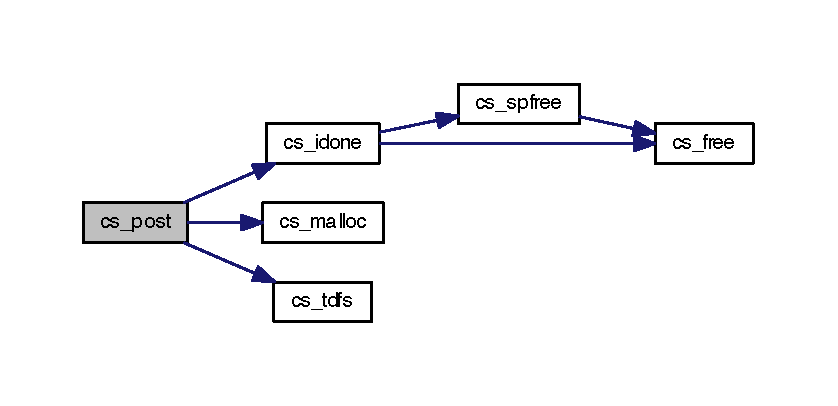
\includegraphics[width=350pt]{csparse_8c_af84bc0a35c099a9a1e01e5aebf8c7292_cgraph}
\end{center}
\end{figure}


\hypertarget{csparse_8c_ab3e2c74ed6cf7521170a45d04aab9b51}{\index{csparse.\-c@{csparse.\-c}!cs\-\_\-print@{cs\-\_\-print}}
\index{cs\-\_\-print@{cs\-\_\-print}!csparse.c@{csparse.\-c}}
\paragraph[{cs\-\_\-print}]{\setlength{\rightskip}{0pt plus 5cm}int cs\-\_\-print (
\begin{DoxyParamCaption}
\item[{const {\bf cs} $\ast$}]{A, }
\item[{int}]{brief}
\end{DoxyParamCaption}
)}}\label{csparse_8c_ab3e2c74ed6cf7521170a45d04aab9b51}


Definition at line 1525 of file csparse.\-c.



References C\-S\-\_\-\-C\-O\-P\-Y\-R\-I\-G\-H\-T, C\-S\-\_\-\-D\-A\-T\-E, cs\-\_\-norm(), C\-S\-\_\-\-S\-U\-B\-S\-U\-B, C\-S\-\_\-\-S\-U\-B\-V\-E\-R, C\-S\-\_\-\-V\-E\-R, cs\-\_\-sparse\-::i, cs\-\_\-sparse\-::m, cs\-\_\-sparse\-::n, cs\-\_\-sparse\-::nz, cs\-\_\-sparse\-::nzmax, cs\-\_\-sparse\-::p, and cs\-\_\-sparse\-::x.



Here is the call graph for this function\-:\nopagebreak
\begin{figure}[H]
\begin{center}
\leavevmode
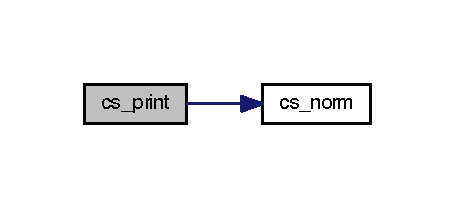
\includegraphics[width=218pt]{csparse_8c_ab3e2c74ed6cf7521170a45d04aab9b51_cgraph}
\end{center}
\end{figure}


\hypertarget{csparse_8c_a547d4d67ec772ecf190dc7073e7fcf41}{\index{csparse.\-c@{csparse.\-c}!cs\-\_\-pvec@{cs\-\_\-pvec}}
\index{cs\-\_\-pvec@{cs\-\_\-pvec}!csparse.c@{csparse.\-c}}
\paragraph[{cs\-\_\-pvec}]{\setlength{\rightskip}{0pt plus 5cm}int cs\-\_\-pvec (
\begin{DoxyParamCaption}
\item[{int}]{n, }
\item[{const int $\ast$}]{P, }
\item[{const double $\ast$}]{b, }
\item[{double $\ast$}]{x}
\end{DoxyParamCaption}
)}}\label{csparse_8c_a547d4d67ec772ecf190dc7073e7fcf41}


Definition at line 1578 of file csparse.\-c.



Referenced by cs\-\_\-cholsol(), and cs\-\_\-qrsol().

\hypertarget{csparse_8c_a767dc90c22d90fe898f72c2da0d98c03}{\index{csparse.\-c@{csparse.\-c}!cs\-\_\-qr@{cs\-\_\-qr}}
\index{cs\-\_\-qr@{cs\-\_\-qr}!csparse.c@{csparse.\-c}}
\paragraph[{cs\-\_\-qr}]{\setlength{\rightskip}{0pt plus 5cm}{\bf csn}$\ast$ cs\-\_\-qr (
\begin{DoxyParamCaption}
\item[{const {\bf cs} $\ast$}]{A, }
\item[{const {\bf css} $\ast$}]{S}
\end{DoxyParamCaption}
)}}\label{csparse_8c_a767dc90c22d90fe898f72c2da0d98c03}


Definition at line 1587 of file csparse.\-c.



References cs\-\_\-numeric\-::\-B, cs\-\_\-calloc(), cs\-\_\-happly(), cs\-\_\-house(), cs\-\_\-malloc(), cs\-\_\-ndone(), cs\-\_\-scatter(), cs\-\_\-spalloc(), cs\-\_\-sparse\-::i, cs\-\_\-numeric\-::\-L, cs\-\_\-symbolic\-::lnz, cs\-\_\-sparse\-::m, cs\-\_\-symbolic\-::m2, cs\-\_\-sparse\-::n, cs\-\_\-sparse\-::p, cs\-\_\-symbolic\-::parent, cs\-\_\-symbolic\-::\-Pinv, cs\-\_\-symbolic\-::\-Q, cs\-\_\-numeric\-::\-U, cs\-\_\-symbolic\-::unz, and cs\-\_\-sparse\-::x.



Referenced by cs\-\_\-qrsol().



Here is the call graph for this function\-:\nopagebreak
\begin{figure}[H]
\begin{center}
\leavevmode
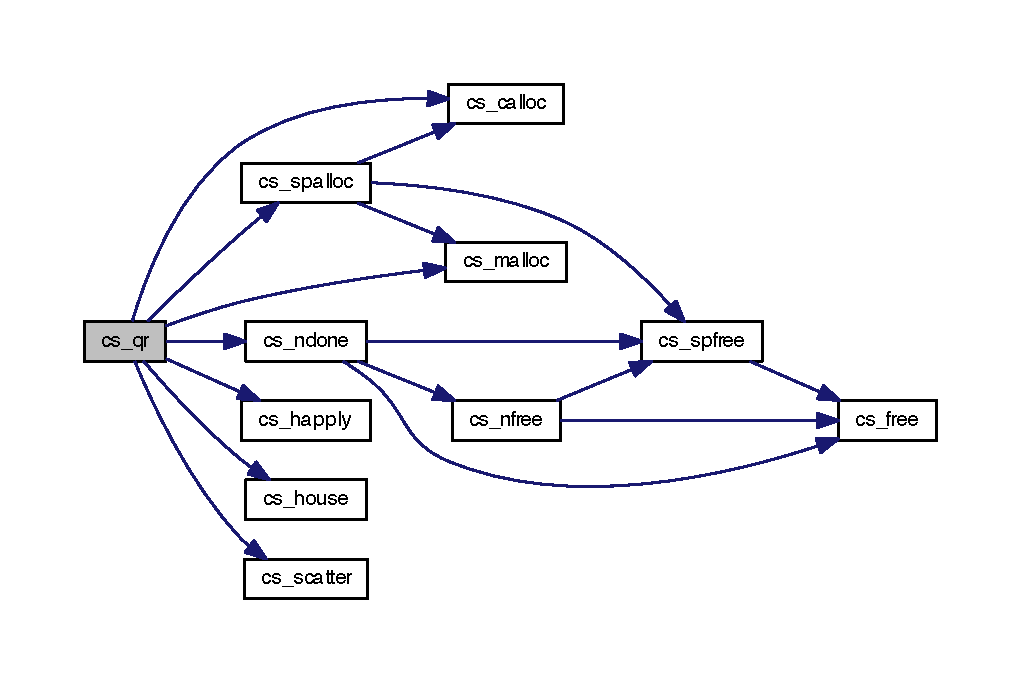
\includegraphics[width=350pt]{csparse_8c_a767dc90c22d90fe898f72c2da0d98c03_cgraph}
\end{center}
\end{figure}


\hypertarget{csparse_8c_a833a289a30d66ea255d49ab3e93c1334}{\index{csparse.\-c@{csparse.\-c}!cs\-\_\-qrsol@{cs\-\_\-qrsol}}
\index{cs\-\_\-qrsol@{cs\-\_\-qrsol}!csparse.c@{csparse.\-c}}
\paragraph[{cs\-\_\-qrsol}]{\setlength{\rightskip}{0pt plus 5cm}int cs\-\_\-qrsol (
\begin{DoxyParamCaption}
\item[{const {\bf cs} $\ast$}]{A, }
\item[{double $\ast$}]{b, }
\item[{int}]{order}
\end{DoxyParamCaption}
)}}\label{csparse_8c_a833a289a30d66ea255d49ab3e93c1334}


Definition at line 1674 of file csparse.\-c.



References cs\-\_\-numeric\-::\-B, cs\-\_\-calloc(), cs\-\_\-free(), cs\-\_\-happly(), cs\-\_\-ipvec(), cs\-\_\-nfree(), cs\-\_\-pvec(), cs\-\_\-qr(), cs\-\_\-sfree(), cs\-\_\-spfree(), cs\-\_\-sqr(), cs\-\_\-transpose(), cs\-\_\-usolve(), cs\-\_\-utsolve(), cs\-\_\-numeric\-::\-L, cs\-\_\-sparse\-::m, cs\-\_\-symbolic\-::m2, cs\-\_\-sparse\-::n, cs\-\_\-symbolic\-::\-Pinv, cs\-\_\-symbolic\-::\-Q, and cs\-\_\-numeric\-::\-U.



Here is the call graph for this function\-:\nopagebreak
\begin{figure}[H]
\begin{center}
\leavevmode
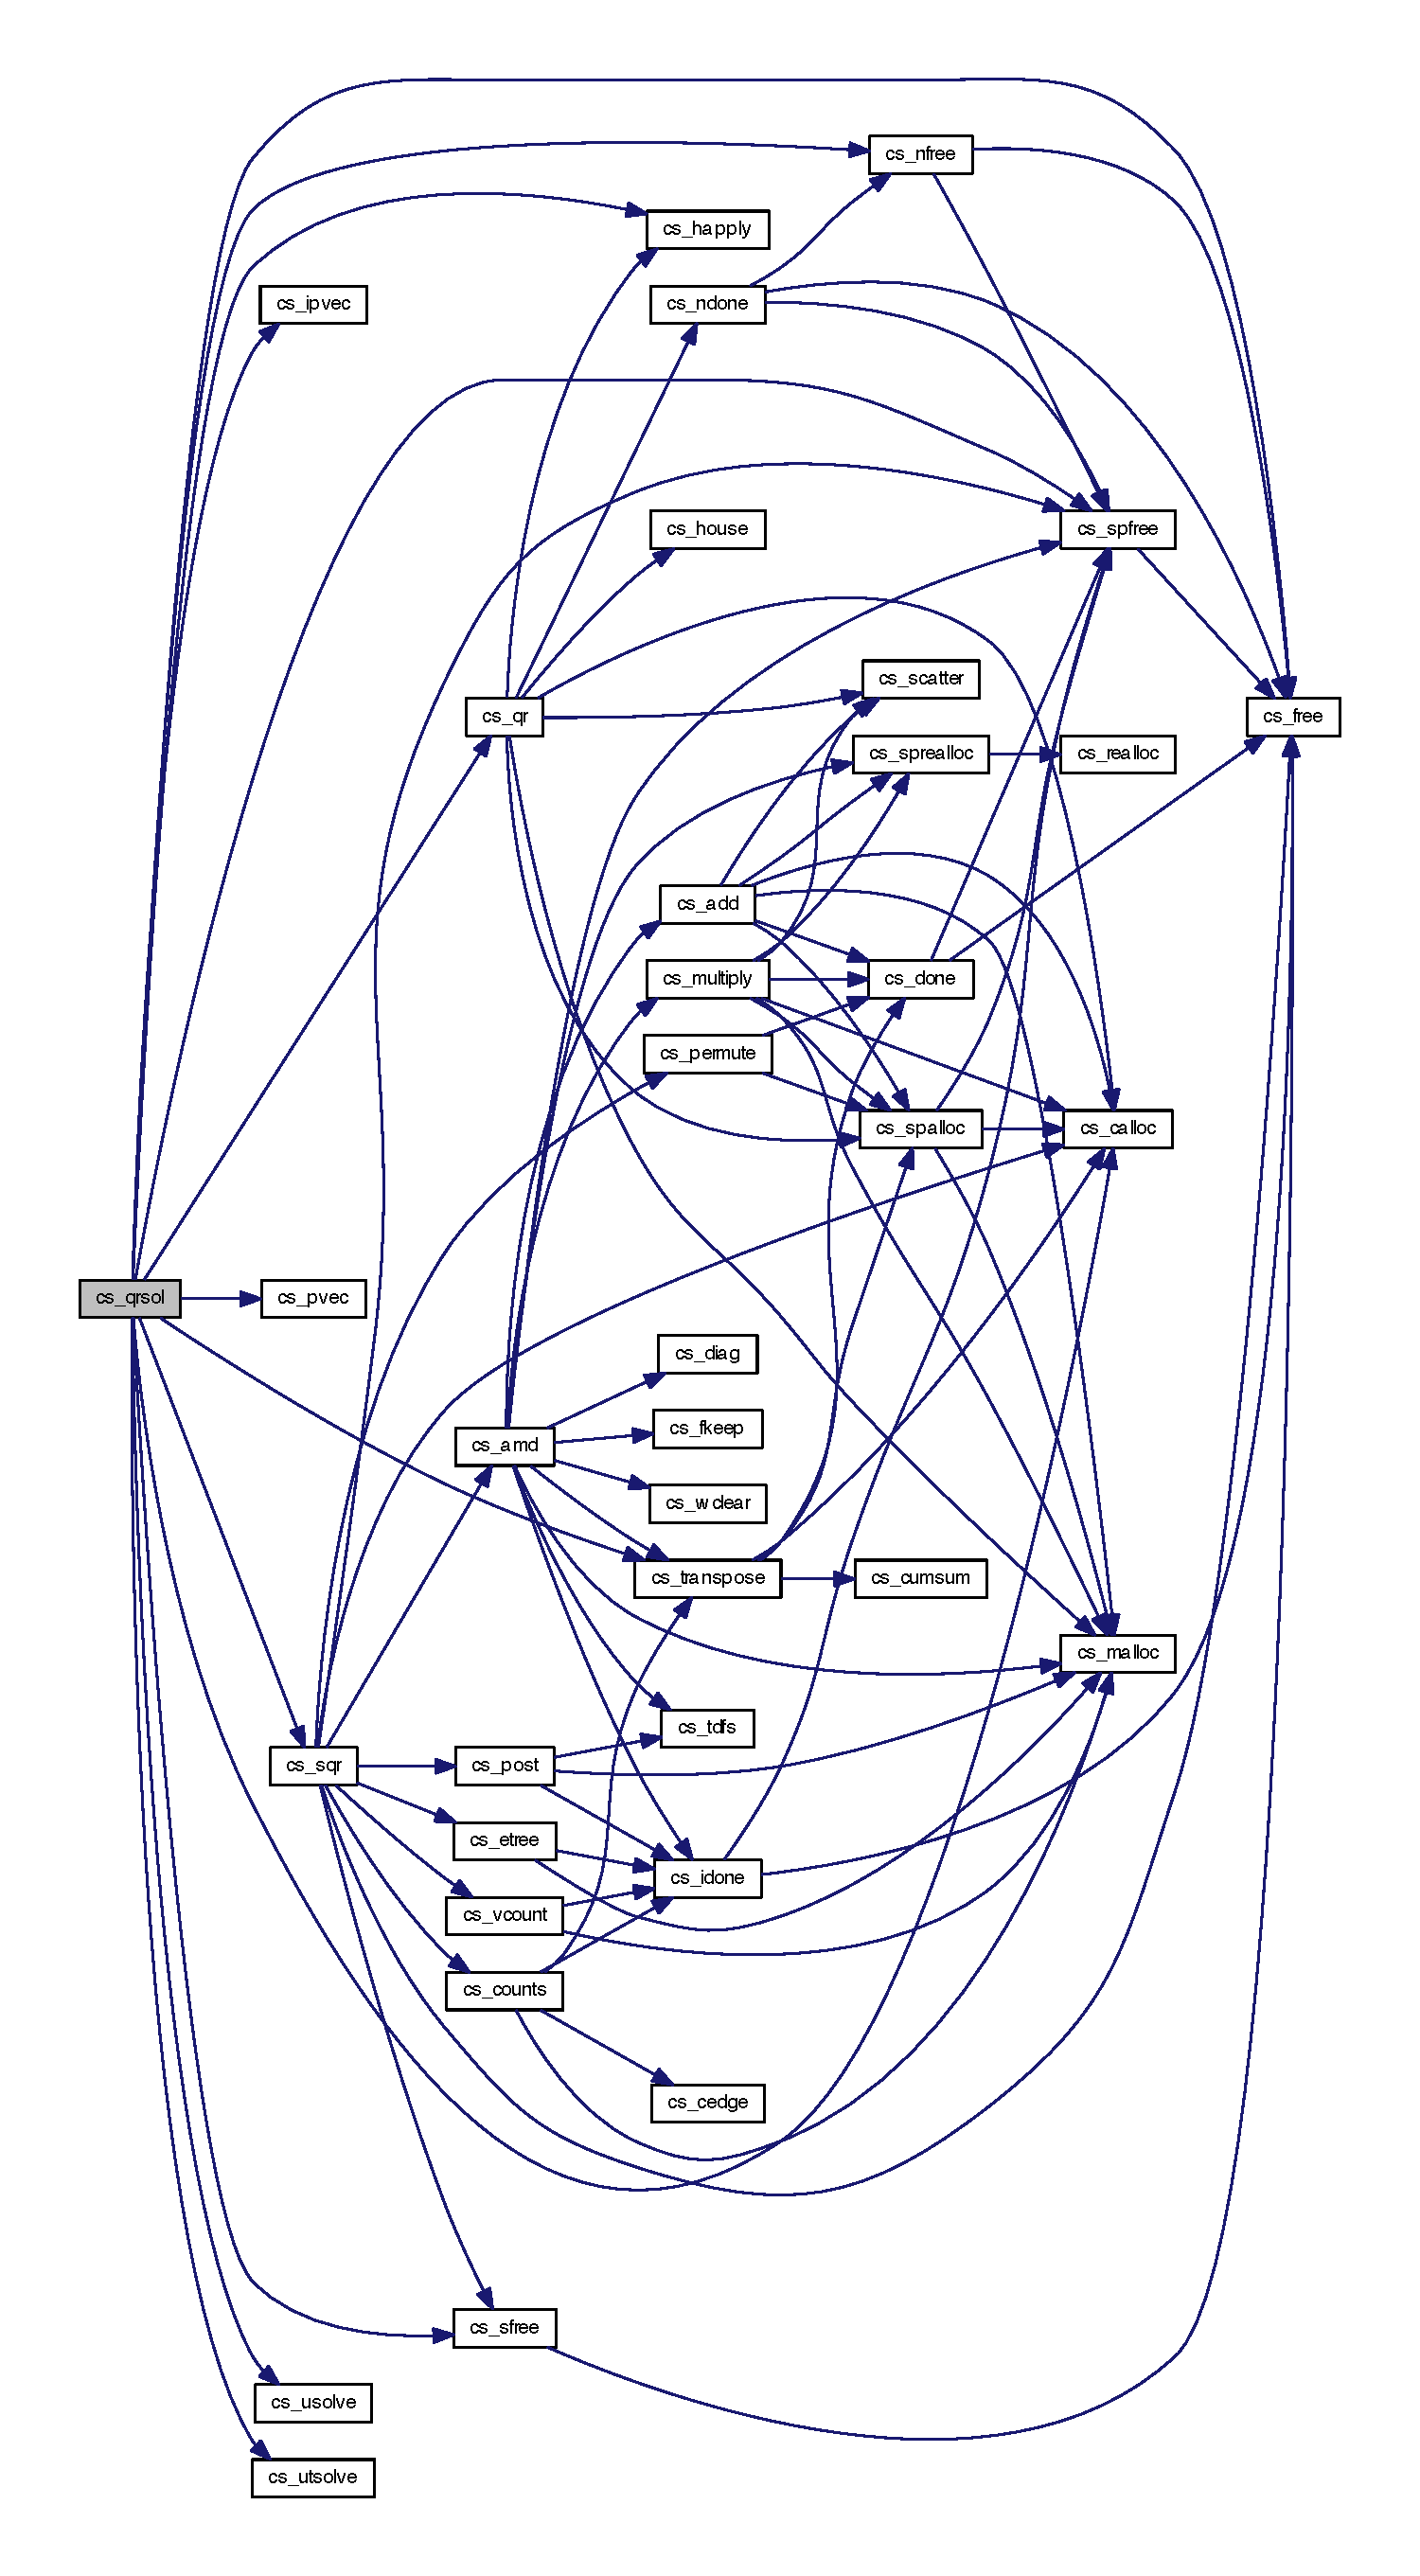
\includegraphics[height=550pt]{csparse_8c_a833a289a30d66ea255d49ab3e93c1334_cgraph}
\end{center}
\end{figure}


\hypertarget{csparse_8c_add4fc69b3887fae610e0362fc13bb214}{\index{csparse.\-c@{csparse.\-c}!cs\-\_\-reach@{cs\-\_\-reach}}
\index{cs\-\_\-reach@{cs\-\_\-reach}!csparse.c@{csparse.\-c}}
\paragraph[{cs\-\_\-reach}]{\setlength{\rightskip}{0pt plus 5cm}int cs\-\_\-reach (
\begin{DoxyParamCaption}
\item[{{\bf cs} $\ast$}]{L, }
\item[{const {\bf cs} $\ast$}]{B, }
\item[{int}]{k, }
\item[{int $\ast$}]{xi, }
\item[{const int $\ast$}]{Pinv}
\end{DoxyParamCaption}
)}}\label{csparse_8c_add4fc69b3887fae610e0362fc13bb214}


Definition at line 1728 of file csparse.\-c.



References cs\-\_\-dfs(), C\-S\-\_\-\-M\-A\-R\-K, C\-S\-\_\-\-M\-A\-R\-K\-E\-D, cs\-\_\-sparse\-::i, cs\-\_\-sparse\-::n, and cs\-\_\-sparse\-::p.



Referenced by cs\-\_\-splsolve().



Here is the call graph for this function\-:\nopagebreak
\begin{figure}[H]
\begin{center}
\leavevmode
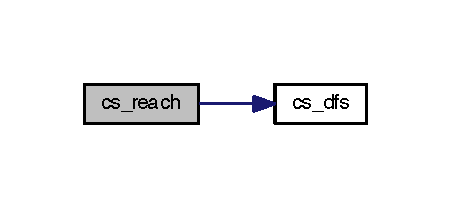
\includegraphics[width=216pt]{csparse_8c_add4fc69b3887fae610e0362fc13bb214_cgraph}
\end{center}
\end{figure}


\hypertarget{csparse_8c_a3729a7e21dbc3309ac96461ddb060328}{\index{csparse.\-c@{csparse.\-c}!cs\-\_\-scatter@{cs\-\_\-scatter}}
\index{cs\-\_\-scatter@{cs\-\_\-scatter}!csparse.c@{csparse.\-c}}
\paragraph[{cs\-\_\-scatter}]{\setlength{\rightskip}{0pt plus 5cm}int cs\-\_\-scatter (
\begin{DoxyParamCaption}
\item[{const {\bf cs} $\ast$}]{A, }
\item[{int}]{j, }
\item[{double}]{beta, }
\item[{int $\ast$}]{w, }
\item[{double $\ast$}]{x, }
\item[{int}]{mark, }
\item[{{\bf cs} $\ast$}]{C, }
\item[{int}]{nz}
\end{DoxyParamCaption}
)}}\label{csparse_8c_a3729a7e21dbc3309ac96461ddb060328}


Definition at line 1749 of file csparse.\-c.



References cs\-\_\-sparse\-::i, cs\-\_\-sparse\-::p, and cs\-\_\-sparse\-::x.



Referenced by cs\-\_\-add(), cs\-\_\-multiply(), and cs\-\_\-qr().

\hypertarget{csparse_8c_a9fede5f7dcf4367d7d005ca6dd0ba100}{\index{csparse.\-c@{csparse.\-c}!cs\-\_\-scc@{cs\-\_\-scc}}
\index{cs\-\_\-scc@{cs\-\_\-scc}!csparse.c@{csparse.\-c}}
\paragraph[{cs\-\_\-scc}]{\setlength{\rightskip}{0pt plus 5cm}{\bf csd}$\ast$ cs\-\_\-scc (
\begin{DoxyParamCaption}
\item[{{\bf cs} $\ast$}]{A}
\end{DoxyParamCaption}
)}}\label{csparse_8c_a9fede5f7dcf4367d7d005ca6dd0ba100}


Definition at line 1774 of file csparse.\-c.



References cs\-\_\-dalloc(), cs\-\_\-ddone(), cs\-\_\-dfs(), cs\-\_\-malloc(), C\-S\-\_\-\-M\-A\-R\-K, C\-S\-\_\-\-M\-A\-R\-K\-E\-D, cs\-\_\-transpose(), cs\-\_\-sparse\-::n, cs\-\_\-dmperm\-\_\-results\-::nb, cs\-\_\-sparse\-::p, cs\-\_\-dmperm\-\_\-results\-::\-P, and cs\-\_\-dmperm\-\_\-results\-::\-R.



Referenced by cs\-\_\-dmperm().



Here is the call graph for this function\-:\nopagebreak
\begin{figure}[H]
\begin{center}
\leavevmode
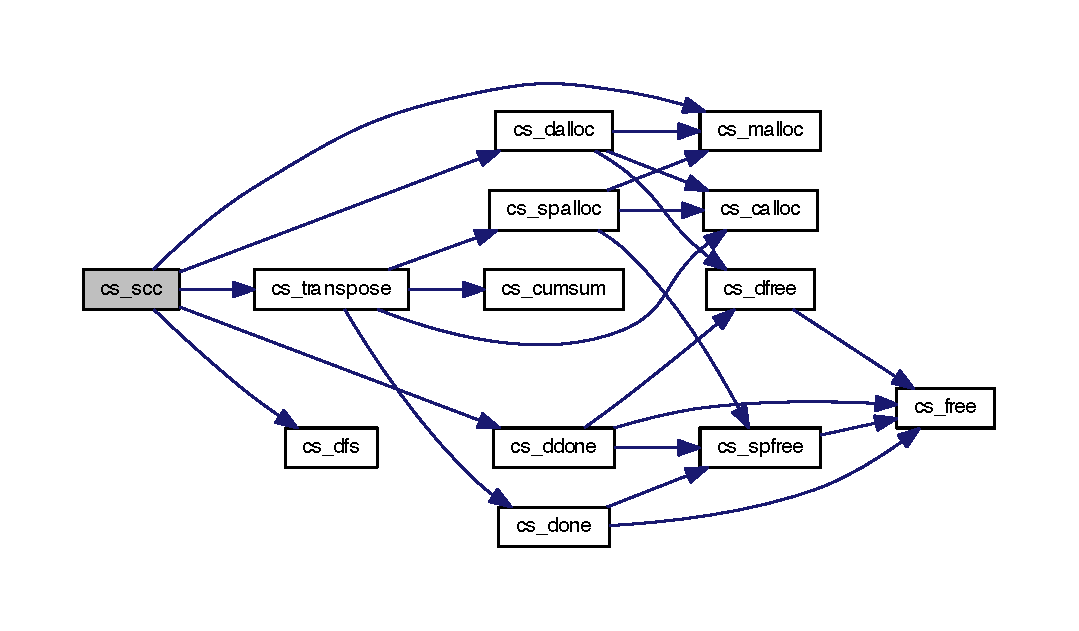
\includegraphics[width=350pt]{csparse_8c_a9fede5f7dcf4367d7d005ca6dd0ba100_cgraph}
\end{center}
\end{figure}


\hypertarget{csparse_8c_afcc0ebf37f4cf80e097ac7e8aa2830f2}{\index{csparse.\-c@{csparse.\-c}!cs\-\_\-schol@{cs\-\_\-schol}}
\index{cs\-\_\-schol@{cs\-\_\-schol}!csparse.c@{csparse.\-c}}
\paragraph[{cs\-\_\-schol}]{\setlength{\rightskip}{0pt plus 5cm}{\bf css}$\ast$ cs\-\_\-schol (
\begin{DoxyParamCaption}
\item[{const {\bf cs} $\ast$}]{A, }
\item[{int}]{order}
\end{DoxyParamCaption}
)}}\label{csparse_8c_afcc0ebf37f4cf80e097ac7e8aa2830f2}


Definition at line 1812 of file csparse.\-c.



References cs\-\_\-symbolic\-::cp, cs\-\_\-amd(), cs\-\_\-calloc(), cs\-\_\-counts(), cs\-\_\-cumsum(), cs\-\_\-etree(), cs\-\_\-free(), cs\-\_\-malloc(), cs\-\_\-pinv(), cs\-\_\-post(), cs\-\_\-sfree(), cs\-\_\-spfree(), cs\-\_\-symperm(), cs\-\_\-symbolic\-::lnz, cs\-\_\-sparse\-::n, cs\-\_\-symbolic\-::parent, cs\-\_\-symbolic\-::\-Pinv, and cs\-\_\-symbolic\-::unz.



Referenced by cs\-\_\-cholsol().



Here is the call graph for this function\-:\nopagebreak
\begin{figure}[H]
\begin{center}
\leavevmode
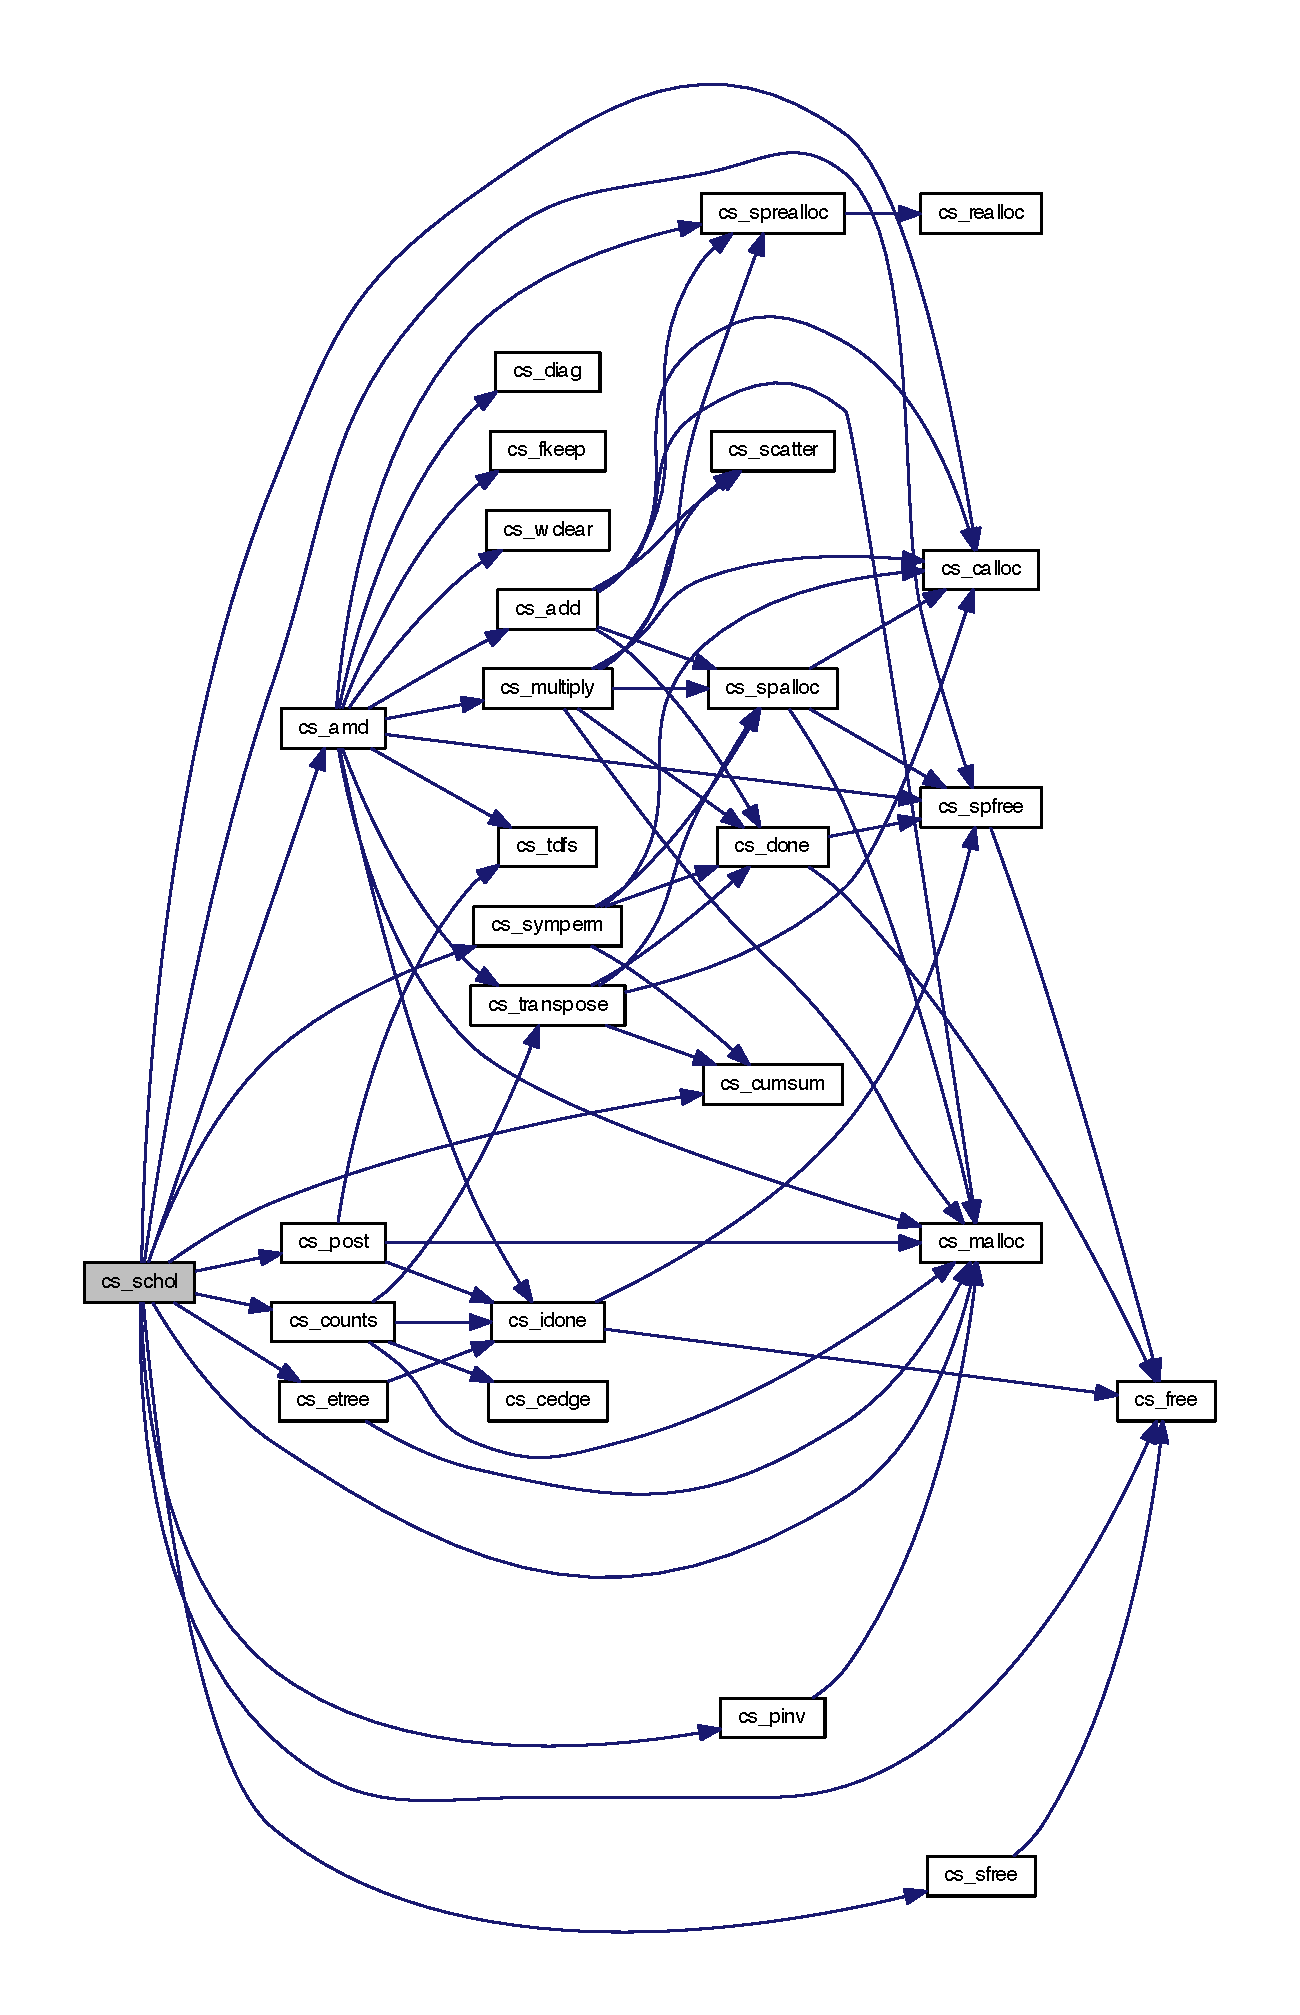
\includegraphics[width=350pt]{csparse_8c_afcc0ebf37f4cf80e097ac7e8aa2830f2_cgraph}
\end{center}
\end{figure}


\hypertarget{csparse_8c_aabed11053c84c540d80e6edc410cce2f}{\index{csparse.\-c@{csparse.\-c}!cs\-\_\-splsolve@{cs\-\_\-splsolve}}
\index{cs\-\_\-splsolve@{cs\-\_\-splsolve}!csparse.c@{csparse.\-c}}
\paragraph[{cs\-\_\-splsolve}]{\setlength{\rightskip}{0pt plus 5cm}int cs\-\_\-splsolve (
\begin{DoxyParamCaption}
\item[{{\bf cs} $\ast$}]{L, }
\item[{const {\bf cs} $\ast$}]{B, }
\item[{int}]{k, }
\item[{int $\ast$}]{xi, }
\item[{double $\ast$}]{x, }
\item[{const int $\ast$}]{Pinv}
\end{DoxyParamCaption}
)}}\label{csparse_8c_aabed11053c84c540d80e6edc410cce2f}


Definition at line 1838 of file csparse.\-c.



References cs\-\_\-reach(), cs\-\_\-sparse\-::i, cs\-\_\-sparse\-::n, cs\-\_\-sparse\-::p, and cs\-\_\-sparse\-::x.



Referenced by cs\-\_\-lu().



Here is the call graph for this function\-:\nopagebreak
\begin{figure}[H]
\begin{center}
\leavevmode
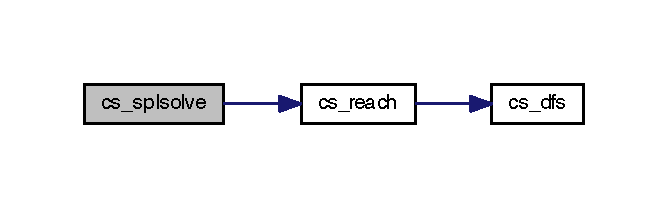
\includegraphics[width=320pt]{csparse_8c_aabed11053c84c540d80e6edc410cce2f_cgraph}
\end{center}
\end{figure}


\hypertarget{csparse_8c_a205fe209b778ab1379668d9037f1e6d7}{\index{csparse.\-c@{csparse.\-c}!cs\-\_\-vcount@{cs\-\_\-vcount}}
\index{cs\-\_\-vcount@{cs\-\_\-vcount}!csparse.c@{csparse.\-c}}
\paragraph[{cs\-\_\-vcount}]{\setlength{\rightskip}{0pt plus 5cm}static int$\ast$ cs\-\_\-vcount (
\begin{DoxyParamCaption}
\item[{const {\bf cs} $\ast$}]{A, }
\item[{const int $\ast$}]{parent, }
\item[{int $\ast$}]{m2, }
\item[{int $\ast$}]{vnz}
\end{DoxyParamCaption}
)\hspace{0.3cm}{\ttfamily [static]}}}\label{csparse_8c_a205fe209b778ab1379668d9037f1e6d7}


Definition at line 1867 of file csparse.\-c.



References cs\-\_\-idone(), cs\-\_\-malloc(), cs\-\_\-sparse\-::i, cs\-\_\-sparse\-::m, cs\-\_\-sparse\-::n, and cs\-\_\-sparse\-::p.



Referenced by cs\-\_\-sqr().



Here is the call graph for this function\-:\nopagebreak
\begin{figure}[H]
\begin{center}
\leavevmode
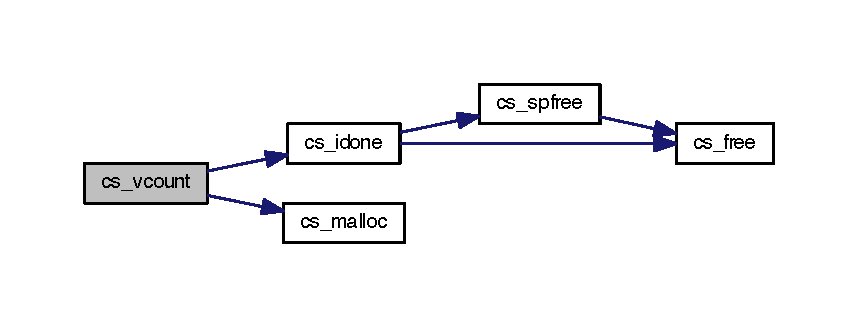
\includegraphics[width=350pt]{csparse_8c_a205fe209b778ab1379668d9037f1e6d7_cgraph}
\end{center}
\end{figure}


\hypertarget{csparse_8c_a0a717b429d68d3c98b6dc8579988473d}{\index{csparse.\-c@{csparse.\-c}!cs\-\_\-sqr@{cs\-\_\-sqr}}
\index{cs\-\_\-sqr@{cs\-\_\-sqr}!csparse.c@{csparse.\-c}}
\paragraph[{cs\-\_\-sqr}]{\setlength{\rightskip}{0pt plus 5cm}{\bf css}$\ast$ cs\-\_\-sqr (
\begin{DoxyParamCaption}
\item[{const {\bf cs} $\ast$}]{A, }
\item[{int}]{order, }
\item[{int}]{qr}
\end{DoxyParamCaption}
)}}\label{csparse_8c_a0a717b429d68d3c98b6dc8579988473d}


Definition at line 1917 of file csparse.\-c.



References cs\-\_\-symbolic\-::cp, cs\-\_\-amd(), cs\-\_\-calloc(), cs\-\_\-counts(), cs\-\_\-etree(), cs\-\_\-free(), cs\-\_\-permute(), cs\-\_\-post(), cs\-\_\-sfree(), cs\-\_\-spfree(), cs\-\_\-vcount(), cs\-\_\-symbolic\-::lnz, cs\-\_\-symbolic\-::m2, cs\-\_\-sparse\-::n, cs\-\_\-sparse\-::p, cs\-\_\-symbolic\-::parent, cs\-\_\-symbolic\-::\-Pinv, cs\-\_\-symbolic\-::\-Q, and cs\-\_\-symbolic\-::unz.



Referenced by cs\-\_\-lusol(), and cs\-\_\-qrsol().



Here is the call graph for this function\-:\nopagebreak
\begin{figure}[H]
\begin{center}
\leavevmode
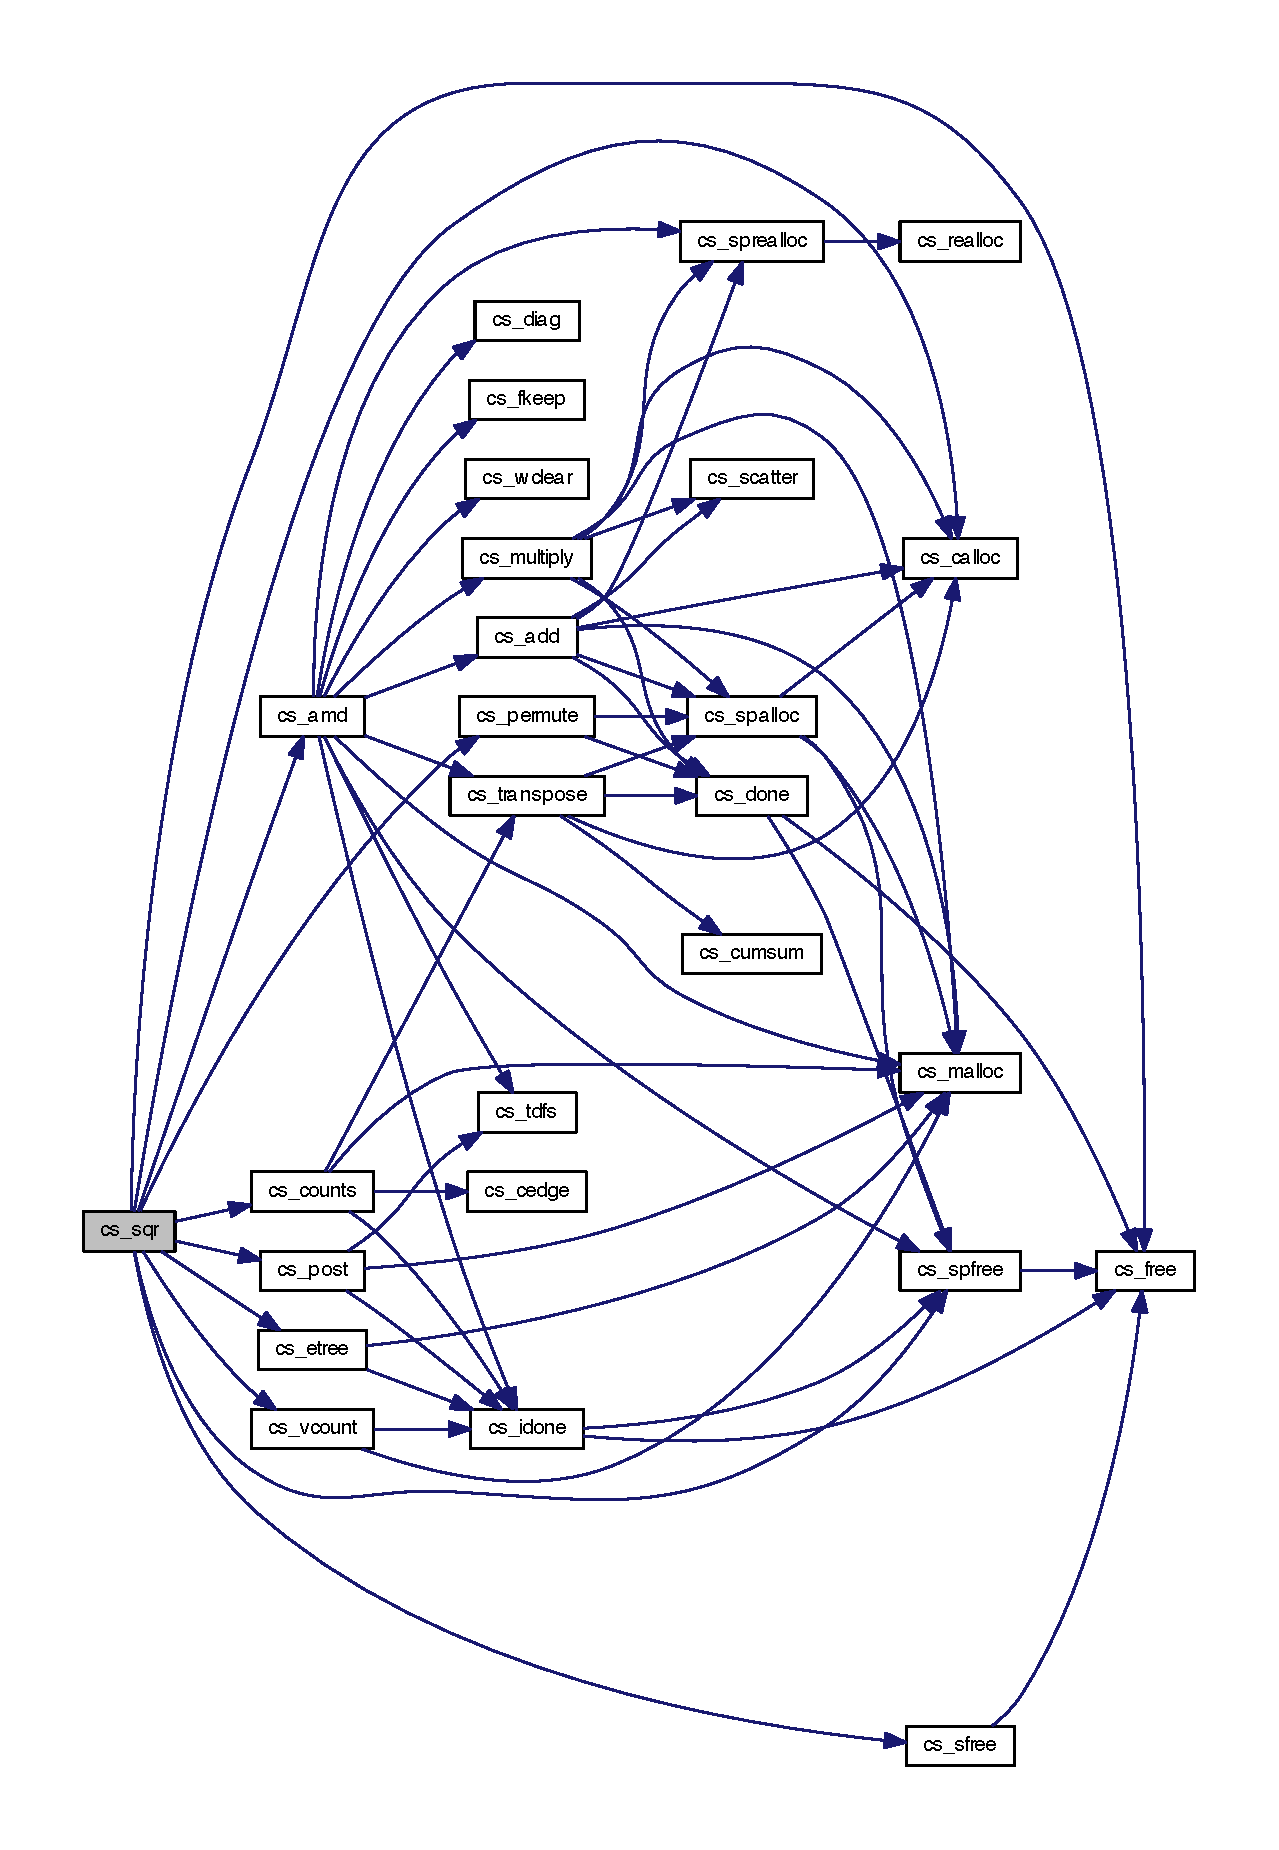
\includegraphics[width=350pt]{csparse_8c_a0a717b429d68d3c98b6dc8579988473d_cgraph}
\end{center}
\end{figure}


\hypertarget{csparse_8c_a6aa95f82cd0d8c61afb033405320d727}{\index{csparse.\-c@{csparse.\-c}!cs\-\_\-symperm@{cs\-\_\-symperm}}
\index{cs\-\_\-symperm@{cs\-\_\-symperm}!csparse.c@{csparse.\-c}}
\paragraph[{cs\-\_\-symperm}]{\setlength{\rightskip}{0pt plus 5cm}{\bf cs}$\ast$ cs\-\_\-symperm (
\begin{DoxyParamCaption}
\item[{const {\bf cs} $\ast$}]{A, }
\item[{const int $\ast$}]{Pinv, }
\item[{int}]{values}
\end{DoxyParamCaption}
)}}\label{csparse_8c_a6aa95f82cd0d8c61afb033405320d727}


Definition at line 1949 of file csparse.\-c.



References cs\-\_\-calloc(), cs\-\_\-cumsum(), cs\-\_\-done(), C\-S\-\_\-\-M\-A\-X, C\-S\-\_\-\-M\-I\-N, cs\-\_\-spalloc(), cs\-\_\-sparse\-::i, cs\-\_\-sparse\-::n, cs\-\_\-sparse\-::p, and cs\-\_\-sparse\-::x.



Referenced by cs\-\_\-chol(), and cs\-\_\-schol().



Here is the call graph for this function\-:\nopagebreak
\begin{figure}[H]
\begin{center}
\leavevmode
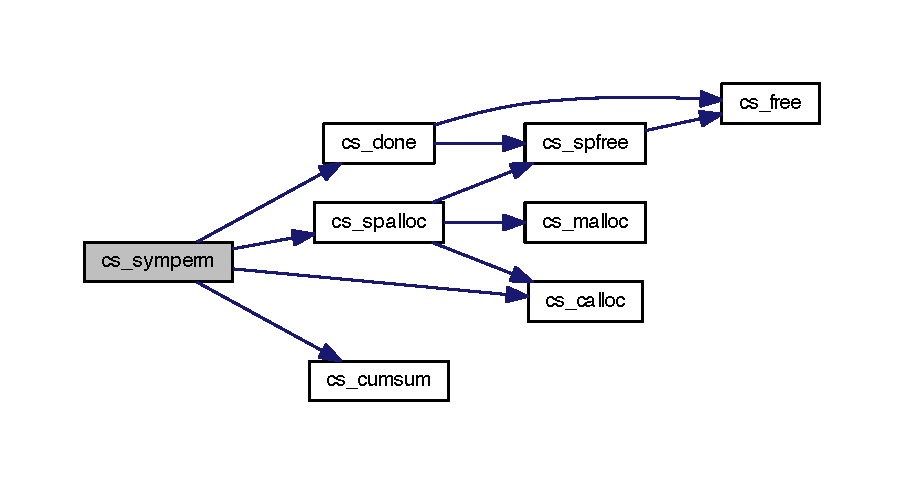
\includegraphics[width=350pt]{csparse_8c_a6aa95f82cd0d8c61afb033405320d727_cgraph}
\end{center}
\end{figure}


\hypertarget{csparse_8c_a7b064c4799cc09da13c13d982197eff7}{\index{csparse.\-c@{csparse.\-c}!cs\-\_\-tdfs@{cs\-\_\-tdfs}}
\index{cs\-\_\-tdfs@{cs\-\_\-tdfs}!csparse.c@{csparse.\-c}}
\paragraph[{cs\-\_\-tdfs}]{\setlength{\rightskip}{0pt plus 5cm}int cs\-\_\-tdfs (
\begin{DoxyParamCaption}
\item[{int}]{j, }
\item[{int}]{k, }
\item[{int $\ast$}]{head, }
\item[{const int $\ast$}]{next, }
\item[{int $\ast$}]{post, }
\item[{int $\ast$}]{stack}
\end{DoxyParamCaption}
)}}\label{csparse_8c_a7b064c4799cc09da13c13d982197eff7}


Definition at line 1993 of file csparse.\-c.



Referenced by cs\-\_\-amd(), and cs\-\_\-post().

\hypertarget{csparse_8c_a090225477a18abe5f8d5ab26e4efaf3a}{\index{csparse.\-c@{csparse.\-c}!cs\-\_\-transpose@{cs\-\_\-transpose}}
\index{cs\-\_\-transpose@{cs\-\_\-transpose}!csparse.c@{csparse.\-c}}
\paragraph[{cs\-\_\-transpose}]{\setlength{\rightskip}{0pt plus 5cm}{\bf cs}$\ast$ cs\-\_\-transpose (
\begin{DoxyParamCaption}
\item[{const {\bf cs} $\ast$}]{A, }
\item[{int}]{values}
\end{DoxyParamCaption}
)}}\label{csparse_8c_a090225477a18abe5f8d5ab26e4efaf3a}


Definition at line 2017 of file csparse.\-c.



References cs\-\_\-calloc(), cs\-\_\-cumsum(), cs\-\_\-done(), cs\-\_\-spalloc(), cs\-\_\-sparse\-::i, cs\-\_\-sparse\-::m, cs\-\_\-sparse\-::n, cs\-\_\-sparse\-::p, and cs\-\_\-sparse\-::x.



Referenced by cs\-\_\-amd(), cs\-\_\-bfs(), cs\-\_\-counts(), cs\-\_\-maxtrans(), cs\-\_\-qrsol(), cs\-\_\-scc(), and fclib\-\_\-merit\-\_\-local().



Here is the call graph for this function\-:\nopagebreak
\begin{figure}[H]
\begin{center}
\leavevmode
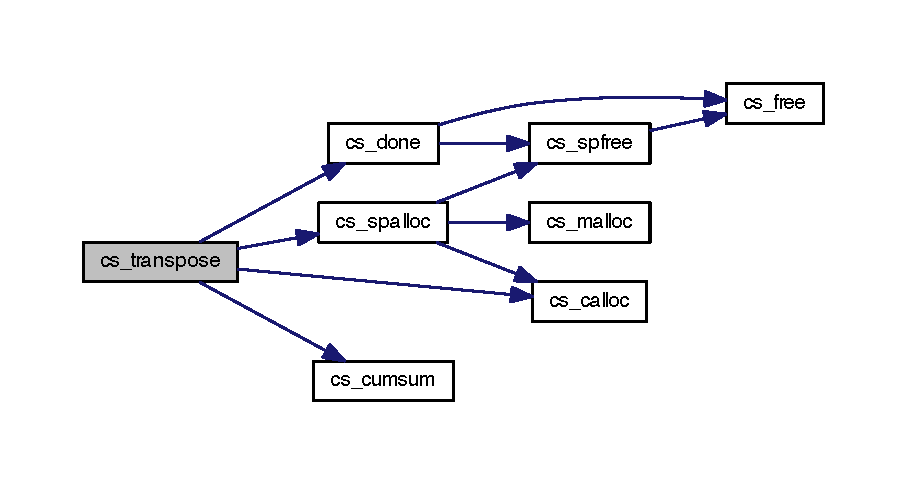
\includegraphics[width=350pt]{csparse_8c_a090225477a18abe5f8d5ab26e4efaf3a_cgraph}
\end{center}
\end{figure}


\hypertarget{csparse_8c_a333e20a0edc2af41f68d77d79ede53e5}{\index{csparse.\-c@{csparse.\-c}!cs\-\_\-triplet@{cs\-\_\-triplet}}
\index{cs\-\_\-triplet@{cs\-\_\-triplet}!csparse.c@{csparse.\-c}}
\paragraph[{cs\-\_\-triplet}]{\setlength{\rightskip}{0pt plus 5cm}{\bf cs}$\ast$ cs\-\_\-triplet (
\begin{DoxyParamCaption}
\item[{const {\bf cs} $\ast$}]{T}
\end{DoxyParamCaption}
)}}\label{csparse_8c_a333e20a0edc2af41f68d77d79ede53e5}


Definition at line 2048 of file csparse.\-c.



References cs\-\_\-calloc(), cs\-\_\-cumsum(), cs\-\_\-done(), cs\-\_\-spalloc(), cs\-\_\-sparse\-::i, cs\-\_\-sparse\-::m, cs\-\_\-sparse\-::n, cs\-\_\-sparse\-::nz, cs\-\_\-sparse\-::p, and cs\-\_\-sparse\-::x.



Here is the call graph for this function\-:\nopagebreak
\begin{figure}[H]
\begin{center}
\leavevmode
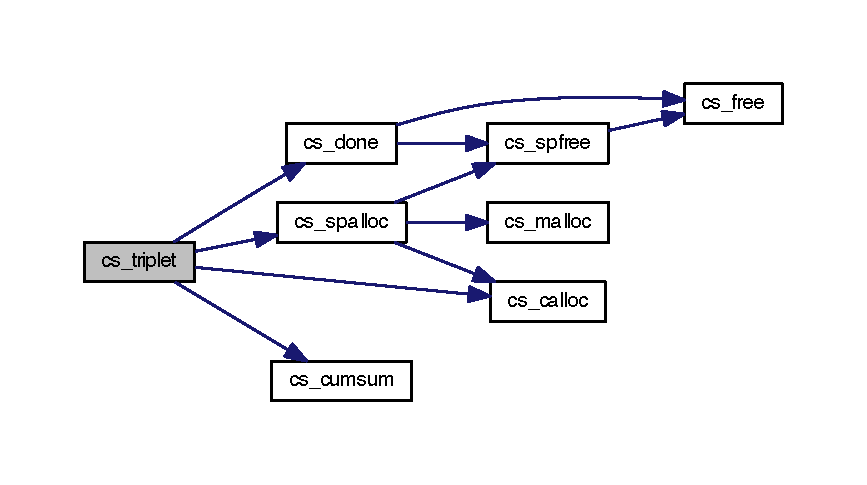
\includegraphics[width=350pt]{csparse_8c_a333e20a0edc2af41f68d77d79ede53e5_cgraph}
\end{center}
\end{figure}


\hypertarget{csparse_8c_ad5fa81f80009c06259a77fd7d2092f78}{\index{csparse.\-c@{csparse.\-c}!cs\-\_\-updown@{cs\-\_\-updown}}
\index{cs\-\_\-updown@{cs\-\_\-updown}!csparse.c@{csparse.\-c}}
\paragraph[{cs\-\_\-updown}]{\setlength{\rightskip}{0pt plus 5cm}int cs\-\_\-updown (
\begin{DoxyParamCaption}
\item[{{\bf cs} $\ast$}]{L, }
\item[{int}]{sigma, }
\item[{const {\bf cs} $\ast$}]{C, }
\item[{const int $\ast$}]{parent}
\end{DoxyParamCaption}
)}}\label{csparse_8c_ad5fa81f80009c06259a77fd7d2092f78}


Definition at line 2077 of file csparse.\-c.



References cs\-\_\-free(), cs\-\_\-malloc(), C\-S\-\_\-\-M\-I\-N, cs\-\_\-sparse\-::i, cs\-\_\-sparse\-::n, cs\-\_\-sparse\-::p, and cs\-\_\-sparse\-::x.



Here is the call graph for this function\-:\nopagebreak
\begin{figure}[H]
\begin{center}
\leavevmode
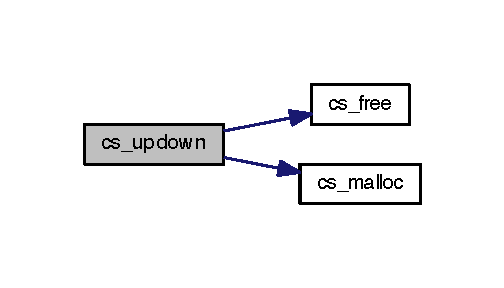
\includegraphics[width=242pt]{csparse_8c_ad5fa81f80009c06259a77fd7d2092f78_cgraph}
\end{center}
\end{figure}


\hypertarget{csparse_8c_aa4cdacecec403b30b97abc7c27594b4f}{\index{csparse.\-c@{csparse.\-c}!cs\-\_\-usolve@{cs\-\_\-usolve}}
\index{cs\-\_\-usolve@{cs\-\_\-usolve}!csparse.c@{csparse.\-c}}
\paragraph[{cs\-\_\-usolve}]{\setlength{\rightskip}{0pt plus 5cm}int cs\-\_\-usolve (
\begin{DoxyParamCaption}
\item[{const {\bf cs} $\ast$}]{U, }
\item[{double $\ast$}]{x}
\end{DoxyParamCaption}
)}}\label{csparse_8c_aa4cdacecec403b30b97abc7c27594b4f}


Definition at line 2119 of file csparse.\-c.



References cs\-\_\-sparse\-::i, cs\-\_\-sparse\-::n, cs\-\_\-sparse\-::p, and cs\-\_\-sparse\-::x.



Referenced by cs\-\_\-lusol(), and cs\-\_\-qrsol().

\hypertarget{csparse_8c_aad3a584d9185a4fe4497a36f892b9c72}{\index{csparse.\-c@{csparse.\-c}!cs\-\_\-spalloc@{cs\-\_\-spalloc}}
\index{cs\-\_\-spalloc@{cs\-\_\-spalloc}!csparse.c@{csparse.\-c}}
\paragraph[{cs\-\_\-spalloc}]{\setlength{\rightskip}{0pt plus 5cm}{\bf cs}$\ast$ cs\-\_\-spalloc (
\begin{DoxyParamCaption}
\item[{int}]{m, }
\item[{int}]{n, }
\item[{int}]{nzmax, }
\item[{int}]{values, }
\item[{int}]{triplet}
\end{DoxyParamCaption}
)}}\label{csparse_8c_aad3a584d9185a4fe4497a36f892b9c72}


Definition at line 2140 of file csparse.\-c.



References cs\-\_\-calloc(), cs\-\_\-malloc(), C\-S\-\_\-\-M\-A\-X, cs\-\_\-spfree(), cs\-\_\-sparse\-::i, cs\-\_\-sparse\-::m, cs\-\_\-sparse\-::n, cs\-\_\-sparse\-::nz, cs\-\_\-sparse\-::nzmax, cs\-\_\-sparse\-::p, and cs\-\_\-sparse\-::x.



Referenced by cs\-\_\-add(), cs\-\_\-chol(), cs\-\_\-load(), cs\-\_\-lu(), cs\-\_\-multiply(), cs\-\_\-permute(), cs\-\_\-qr(), cs\-\_\-symperm(), cs\-\_\-transpose(), and cs\-\_\-triplet().



Here is the call graph for this function\-:\nopagebreak
\begin{figure}[H]
\begin{center}
\leavevmode
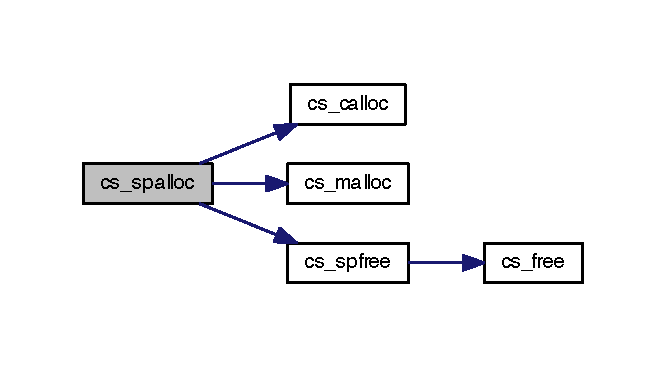
\includegraphics[width=320pt]{csparse_8c_aad3a584d9185a4fe4497a36f892b9c72_cgraph}
\end{center}
\end{figure}


\hypertarget{csparse_8c_a5a9bc4224732ce1cedc50119afc687c1}{\index{csparse.\-c@{csparse.\-c}!cs\-\_\-sprealloc@{cs\-\_\-sprealloc}}
\index{cs\-\_\-sprealloc@{cs\-\_\-sprealloc}!csparse.c@{csparse.\-c}}
\paragraph[{cs\-\_\-sprealloc}]{\setlength{\rightskip}{0pt plus 5cm}int cs\-\_\-sprealloc (
\begin{DoxyParamCaption}
\item[{{\bf cs} $\ast$}]{A, }
\item[{int}]{nzmax}
\end{DoxyParamCaption}
)}}\label{csparse_8c_a5a9bc4224732ce1cedc50119afc687c1}


Definition at line 2155 of file csparse.\-c.



References cs\-\_\-realloc(), cs\-\_\-sparse\-::i, cs\-\_\-sparse\-::n, cs\-\_\-sparse\-::nz, cs\-\_\-sparse\-::nzmax, cs\-\_\-sparse\-::p, and cs\-\_\-sparse\-::x.



Referenced by cs\-\_\-add(), cs\-\_\-amd(), cs\-\_\-dupl(), cs\-\_\-entry(), cs\-\_\-lu(), and cs\-\_\-multiply().



Here is the call graph for this function\-:\nopagebreak
\begin{figure}[H]
\begin{center}
\leavevmode
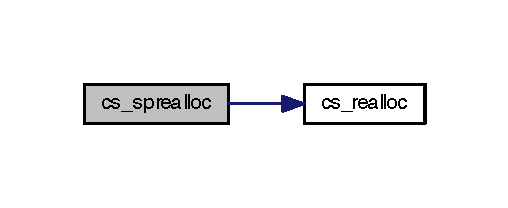
\includegraphics[width=244pt]{csparse_8c_a5a9bc4224732ce1cedc50119afc687c1_cgraph}
\end{center}
\end{figure}


\hypertarget{csparse_8c_a6d705e404a7831ccf01bc0ea064215b9}{\index{csparse.\-c@{csparse.\-c}!cs\-\_\-spfree@{cs\-\_\-spfree}}
\index{cs\-\_\-spfree@{cs\-\_\-spfree}!csparse.c@{csparse.\-c}}
\paragraph[{cs\-\_\-spfree}]{\setlength{\rightskip}{0pt plus 5cm}{\bf cs}$\ast$ cs\-\_\-spfree (
\begin{DoxyParamCaption}
\item[{{\bf cs} $\ast$}]{A}
\end{DoxyParamCaption}
)}}\label{csparse_8c_a6d705e404a7831ccf01bc0ea064215b9}


Definition at line 2169 of file csparse.\-c.



References cs\-\_\-free(), cs\-\_\-sparse\-::i, cs\-\_\-sparse\-::p, and cs\-\_\-sparse\-::x.



Referenced by cs\-\_\-amd(), cs\-\_\-bfs(), cs\-\_\-ddone(), cs\-\_\-done(), cs\-\_\-idone(), cs\-\_\-load(), cs\-\_\-ndone(), cs\-\_\-nfree(), cs\-\_\-qrsol(), cs\-\_\-schol(), cs\-\_\-spalloc(), and cs\-\_\-sqr().



Here is the call graph for this function\-:\nopagebreak
\begin{figure}[H]
\begin{center}
\leavevmode
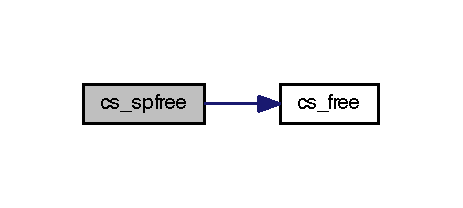
\includegraphics[width=222pt]{csparse_8c_a6d705e404a7831ccf01bc0ea064215b9_cgraph}
\end{center}
\end{figure}


\hypertarget{csparse_8c_af2e6d75dfc24a842fdbce3aa510dc4bc}{\index{csparse.\-c@{csparse.\-c}!cs\-\_\-nfree@{cs\-\_\-nfree}}
\index{cs\-\_\-nfree@{cs\-\_\-nfree}!csparse.c@{csparse.\-c}}
\paragraph[{cs\-\_\-nfree}]{\setlength{\rightskip}{0pt plus 5cm}{\bf csn}$\ast$ cs\-\_\-nfree (
\begin{DoxyParamCaption}
\item[{{\bf csn} $\ast$}]{N}
\end{DoxyParamCaption}
)}}\label{csparse_8c_af2e6d75dfc24a842fdbce3aa510dc4bc}


Definition at line 2179 of file csparse.\-c.



References cs\-\_\-numeric\-::\-B, cs\-\_\-free(), cs\-\_\-spfree(), cs\-\_\-numeric\-::\-L, cs\-\_\-numeric\-::\-Pinv, and cs\-\_\-numeric\-::\-U.



Referenced by cs\-\_\-cholsol(), cs\-\_\-lusol(), cs\-\_\-ndone(), and cs\-\_\-qrsol().



Here is the call graph for this function\-:\nopagebreak
\begin{figure}[H]
\begin{center}
\leavevmode
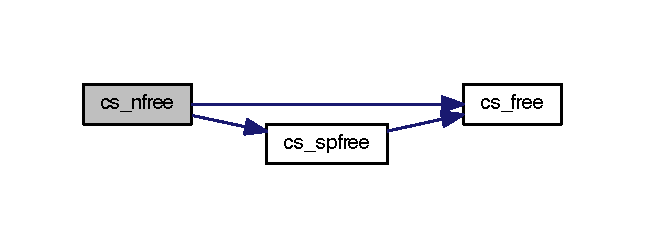
\includegraphics[width=310pt]{csparse_8c_af2e6d75dfc24a842fdbce3aa510dc4bc_cgraph}
\end{center}
\end{figure}


\hypertarget{csparse_8c_ace766075ef439ad6e4347f6b076eb4b7}{\index{csparse.\-c@{csparse.\-c}!cs\-\_\-sfree@{cs\-\_\-sfree}}
\index{cs\-\_\-sfree@{cs\-\_\-sfree}!csparse.c@{csparse.\-c}}
\paragraph[{cs\-\_\-sfree}]{\setlength{\rightskip}{0pt plus 5cm}{\bf css}$\ast$ cs\-\_\-sfree (
\begin{DoxyParamCaption}
\item[{{\bf css} $\ast$}]{S}
\end{DoxyParamCaption}
)}}\label{csparse_8c_ace766075ef439ad6e4347f6b076eb4b7}


Definition at line 2190 of file csparse.\-c.



References cs\-\_\-symbolic\-::cp, cs\-\_\-free(), cs\-\_\-symbolic\-::parent, cs\-\_\-symbolic\-::\-Pinv, and cs\-\_\-symbolic\-::\-Q.



Referenced by cs\-\_\-cholsol(), cs\-\_\-lusol(), cs\-\_\-qrsol(), cs\-\_\-schol(), and cs\-\_\-sqr().



Here is the call graph for this function\-:\nopagebreak
\begin{figure}[H]
\begin{center}
\leavevmode
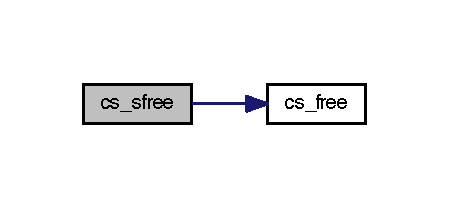
\includegraphics[width=216pt]{csparse_8c_ace766075ef439ad6e4347f6b076eb4b7_cgraph}
\end{center}
\end{figure}


\hypertarget{csparse_8c_aefbcfeb2d1143578988d22d116dde57b}{\index{csparse.\-c@{csparse.\-c}!cs\-\_\-dalloc@{cs\-\_\-dalloc}}
\index{cs\-\_\-dalloc@{cs\-\_\-dalloc}!csparse.c@{csparse.\-c}}
\paragraph[{cs\-\_\-dalloc}]{\setlength{\rightskip}{0pt plus 5cm}{\bf csd}$\ast$ cs\-\_\-dalloc (
\begin{DoxyParamCaption}
\item[{int}]{m, }
\item[{int}]{n}
\end{DoxyParamCaption}
)}}\label{csparse_8c_aefbcfeb2d1143578988d22d116dde57b}


Definition at line 2201 of file csparse.\-c.



References cs\-\_\-calloc(), cs\-\_\-dfree(), cs\-\_\-malloc(), cs\-\_\-dmperm\-\_\-results\-::\-P, cs\-\_\-dmperm\-\_\-results\-::\-Q, cs\-\_\-dmperm\-\_\-results\-::\-R, and cs\-\_\-dmperm\-\_\-results\-::\-S.



Referenced by cs\-\_\-dmperm(), and cs\-\_\-scc().



Here is the call graph for this function\-:\nopagebreak
\begin{figure}[H]
\begin{center}
\leavevmode
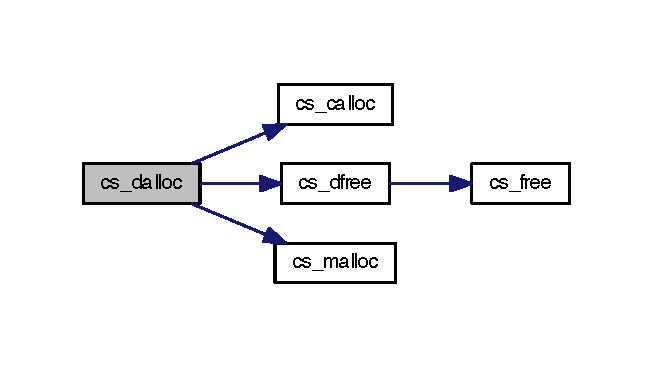
\includegraphics[width=314pt]{csparse_8c_aefbcfeb2d1143578988d22d116dde57b_cgraph}
\end{center}
\end{figure}


\hypertarget{csparse_8c_a7c59264397d2c5cc85c87c879aedc4f5}{\index{csparse.\-c@{csparse.\-c}!cs\-\_\-dfree@{cs\-\_\-dfree}}
\index{cs\-\_\-dfree@{cs\-\_\-dfree}!csparse.c@{csparse.\-c}}
\paragraph[{cs\-\_\-dfree}]{\setlength{\rightskip}{0pt plus 5cm}{\bf csd}$\ast$ cs\-\_\-dfree (
\begin{DoxyParamCaption}
\item[{{\bf csd} $\ast$}]{D}
\end{DoxyParamCaption}
)}}\label{csparse_8c_a7c59264397d2c5cc85c87c879aedc4f5}


Definition at line 2214 of file csparse.\-c.



References cs\-\_\-free(), cs\-\_\-dmperm\-\_\-results\-::\-P, cs\-\_\-dmperm\-\_\-results\-::\-Q, cs\-\_\-dmperm\-\_\-results\-::\-R, and cs\-\_\-dmperm\-\_\-results\-::\-S.



Referenced by cs\-\_\-dalloc(), cs\-\_\-ddone(), and cs\-\_\-dmperm().



Here is the call graph for this function\-:\nopagebreak
\begin{figure}[H]
\begin{center}
\leavevmode
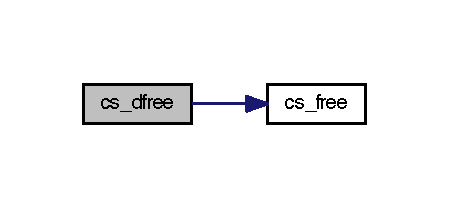
\includegraphics[width=216pt]{csparse_8c_a7c59264397d2c5cc85c87c879aedc4f5_cgraph}
\end{center}
\end{figure}


\hypertarget{csparse_8c_a41590e7ef8c8f3ebce8c7bbe07303c28}{\index{csparse.\-c@{csparse.\-c}!cs\-\_\-done@{cs\-\_\-done}}
\index{cs\-\_\-done@{cs\-\_\-done}!csparse.c@{csparse.\-c}}
\paragraph[{cs\-\_\-done}]{\setlength{\rightskip}{0pt plus 5cm}{\bf cs}$\ast$ cs\-\_\-done (
\begin{DoxyParamCaption}
\item[{{\bf cs} $\ast$}]{C, }
\item[{void $\ast$}]{w, }
\item[{void $\ast$}]{x, }
\item[{int}]{ok}
\end{DoxyParamCaption}
)}}\label{csparse_8c_a41590e7ef8c8f3ebce8c7bbe07303c28}


Definition at line 2225 of file csparse.\-c.



References cs\-\_\-free(), and cs\-\_\-spfree().



Referenced by cs\-\_\-add(), cs\-\_\-multiply(), cs\-\_\-permute(), cs\-\_\-symperm(), cs\-\_\-transpose(), and cs\-\_\-triplet().



Here is the call graph for this function\-:\nopagebreak
\begin{figure}[H]
\begin{center}
\leavevmode
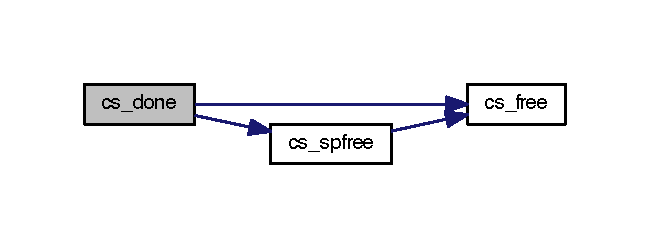
\includegraphics[width=312pt]{csparse_8c_a41590e7ef8c8f3ebce8c7bbe07303c28_cgraph}
\end{center}
\end{figure}


\hypertarget{csparse_8c_a9c3bd8e36cdfb832d199b580e22467c7}{\index{csparse.\-c@{csparse.\-c}!cs\-\_\-idone@{cs\-\_\-idone}}
\index{cs\-\_\-idone@{cs\-\_\-idone}!csparse.c@{csparse.\-c}}
\paragraph[{cs\-\_\-idone}]{\setlength{\rightskip}{0pt plus 5cm}int$\ast$ cs\-\_\-idone (
\begin{DoxyParamCaption}
\item[{int $\ast$}]{p, }
\item[{{\bf cs} $\ast$}]{C, }
\item[{void $\ast$}]{w, }
\item[{int}]{ok}
\end{DoxyParamCaption}
)}}\label{csparse_8c_a9c3bd8e36cdfb832d199b580e22467c7}


Definition at line 2233 of file csparse.\-c.



References cs\-\_\-free(), and cs\-\_\-spfree().



Referenced by cs\-\_\-amd(), cs\-\_\-counts(), cs\-\_\-etree(), cs\-\_\-maxtrans(), cs\-\_\-post(), and cs\-\_\-vcount().



Here is the call graph for this function\-:\nopagebreak
\begin{figure}[H]
\begin{center}
\leavevmode
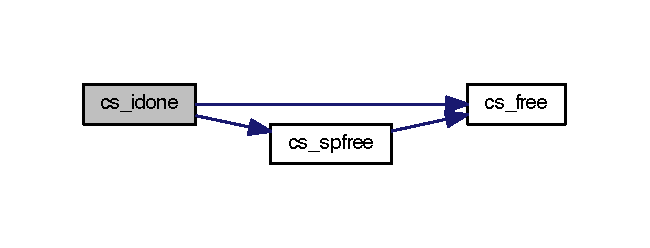
\includegraphics[width=312pt]{csparse_8c_a9c3bd8e36cdfb832d199b580e22467c7_cgraph}
\end{center}
\end{figure}


\hypertarget{csparse_8c_a24796e2f78414578fd2b8e7528535cbb}{\index{csparse.\-c@{csparse.\-c}!cs\-\_\-ndone@{cs\-\_\-ndone}}
\index{cs\-\_\-ndone@{cs\-\_\-ndone}!csparse.c@{csparse.\-c}}
\paragraph[{cs\-\_\-ndone}]{\setlength{\rightskip}{0pt plus 5cm}{\bf csn}$\ast$ cs\-\_\-ndone (
\begin{DoxyParamCaption}
\item[{{\bf csn} $\ast$}]{N, }
\item[{{\bf cs} $\ast$}]{C, }
\item[{void $\ast$}]{w, }
\item[{void $\ast$}]{x, }
\item[{int}]{ok}
\end{DoxyParamCaption}
)}}\label{csparse_8c_a24796e2f78414578fd2b8e7528535cbb}


Definition at line 2241 of file csparse.\-c.



References cs\-\_\-free(), cs\-\_\-nfree(), and cs\-\_\-spfree().



Referenced by cs\-\_\-chol(), cs\-\_\-lu(), and cs\-\_\-qr().



Here is the call graph for this function\-:\nopagebreak
\begin{figure}[H]
\begin{center}
\leavevmode
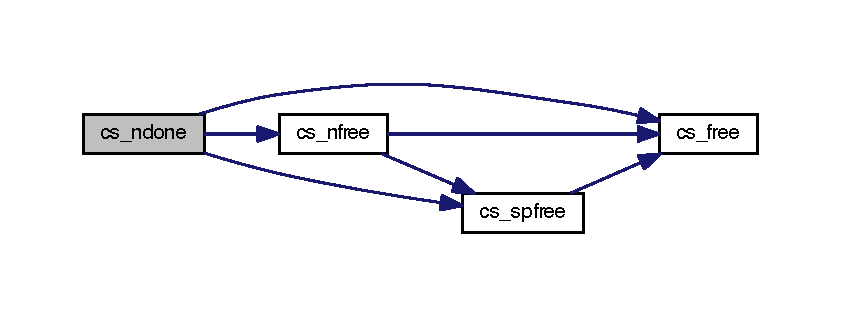
\includegraphics[width=350pt]{csparse_8c_a24796e2f78414578fd2b8e7528535cbb_cgraph}
\end{center}
\end{figure}


\hypertarget{csparse_8c_a312cb23797ac49cd9e99853f6bd2895f}{\index{csparse.\-c@{csparse.\-c}!cs\-\_\-ddone@{cs\-\_\-ddone}}
\index{cs\-\_\-ddone@{cs\-\_\-ddone}!csparse.c@{csparse.\-c}}
\paragraph[{cs\-\_\-ddone}]{\setlength{\rightskip}{0pt plus 5cm}{\bf csd}$\ast$ cs\-\_\-ddone (
\begin{DoxyParamCaption}
\item[{{\bf csd} $\ast$}]{D, }
\item[{{\bf cs} $\ast$}]{C, }
\item[{void $\ast$}]{w, }
\item[{int}]{ok}
\end{DoxyParamCaption}
)}}\label{csparse_8c_a312cb23797ac49cd9e99853f6bd2895f}


Definition at line 2250 of file csparse.\-c.



References cs\-\_\-dfree(), cs\-\_\-free(), and cs\-\_\-spfree().



Referenced by cs\-\_\-dmperm(), and cs\-\_\-scc().



Here is the call graph for this function\-:\nopagebreak
\begin{figure}[H]
\begin{center}
\leavevmode
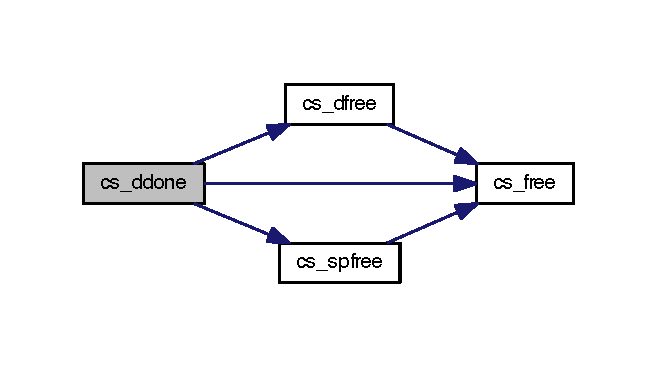
\includegraphics[width=316pt]{csparse_8c_a312cb23797ac49cd9e99853f6bd2895f_cgraph}
\end{center}
\end{figure}


\hypertarget{csparse_8c_a9fbb54471515f219326666ffc4e3e255}{\index{csparse.\-c@{csparse.\-c}!cs\-\_\-utsolve@{cs\-\_\-utsolve}}
\index{cs\-\_\-utsolve@{cs\-\_\-utsolve}!csparse.c@{csparse.\-c}}
\paragraph[{cs\-\_\-utsolve}]{\setlength{\rightskip}{0pt plus 5cm}int cs\-\_\-utsolve (
\begin{DoxyParamCaption}
\item[{const {\bf cs} $\ast$}]{U, }
\item[{double $\ast$}]{x}
\end{DoxyParamCaption}
)}}\label{csparse_8c_a9fbb54471515f219326666ffc4e3e255}


Definition at line 2258 of file csparse.\-c.



References cs\-\_\-sparse\-::i, cs\-\_\-sparse\-::n, cs\-\_\-sparse\-::p, and cs\-\_\-sparse\-::x.



Referenced by cs\-\_\-qrsol().


\hypertarget{csparse_8h}{\subsection{csparse.\-h File Reference}
\label{csparse_8h}\index{csparse.\-h@{csparse.\-h}}
}
This graph shows which files directly or indirectly include this file\-:\nopagebreak
\begin{figure}[H]
\begin{center}
\leavevmode
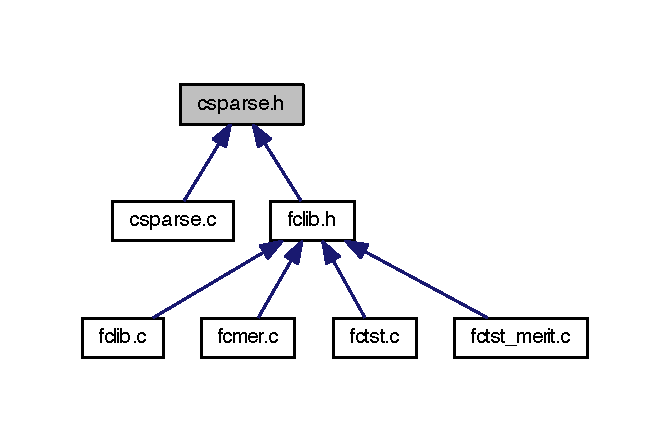
\includegraphics[width=322pt]{csparse_8h__dep__incl}
\end{center}
\end{figure}
\subsubsection*{Classes}
\begin{DoxyCompactItemize}
\item 
struct \hyperlink{structcs__sparse}{cs\-\_\-sparse}
\item 
struct \hyperlink{structcs__symbolic}{cs\-\_\-symbolic}
\item 
struct \hyperlink{structcs__numeric}{cs\-\_\-numeric}
\item 
struct \hyperlink{structcs__dmperm__results}{cs\-\_\-dmperm\-\_\-results}
\end{DoxyCompactItemize}
\subsubsection*{Macros}
\begin{DoxyCompactItemize}
\item 
\#define \hyperlink{csparse_8h_a4371903ff8b39a742cfaf6c6d7f60c4b}{C\-S\-\_\-\-V\-E\-R}~1		    /$\ast$ C\-Sparse Version 1.\-2.\-0 $\ast$/
\item 
\#define \hyperlink{csparse_8h_ac86012ab063a9b8248eaac8bec3b648b}{C\-S\-\_\-\-S\-U\-B\-V\-E\-R}~2
\item 
\#define \hyperlink{csparse_8h_a7f63c57bd63a43fe7ca98e82f524f2ea}{C\-S\-\_\-\-S\-U\-B\-S\-U\-B}~0
\item 
\#define \hyperlink{csparse_8h_a368a611d92ef4a9df9b95cfad8dccf80}{C\-S\-\_\-\-D\-A\-T\-E}~\char`\"{}Mar 6, 2006\char`\"{}	    /$\ast$ C\-Sparse release date $\ast$/
\item 
\#define \hyperlink{csparse_8h_ae6b1a40644b8ddacbbc3bd7c255dbbb4}{C\-S\-\_\-\-C\-O\-P\-Y\-R\-I\-G\-H\-T}~\char`\"{}Copyright (c) Timothy A. Davis, 2006\char`\"{}
\item 
\#define \hyperlink{csparse_8h_a7447e0bed6bf453743551d158e019e8b}{C\-S\-\_\-\-M\-A\-X}(a, b)~(((a) $>$ (b)) ? (a) \-: (b))
\item 
\#define \hyperlink{csparse_8h_a2635aa5c35f05bb0e4c88be5aabae949}{C\-S\-\_\-\-M\-I\-N}(a, b)~(((a) $<$ (b)) ? (a) \-: (b))
\item 
\#define \hyperlink{csparse_8h_aa64f99348d6e0bd00fd5f974199b685a}{C\-S\-\_\-\-F\-L\-I\-P}(i)~(-\/(i)-\/2)
\item 
\#define \hyperlink{csparse_8h_ac9ba6b1092f27aeed7f94a418610aff9}{C\-S\-\_\-\-U\-N\-F\-L\-I\-P}(i)~(((i) $<$ 0) ? \hyperlink{csparse_8h_aa64f99348d6e0bd00fd5f974199b685a}{C\-S\-\_\-\-F\-L\-I\-P}(i) \-: (i))
\item 
\#define \hyperlink{csparse_8h_a434539b758c06b28c4e62ad2a56b859b}{C\-S\-\_\-\-M\-A\-R\-K\-E\-D}(Ap, j)~(Ap \mbox{[}j\mbox{]} $<$ 0)
\item 
\#define \hyperlink{csparse_8h_a8c9d2b0aa06c83acbaf8a183d76e4e2c}{C\-S\-\_\-\-M\-A\-R\-K}(Ap, j)~\{ Ap \mbox{[}j\mbox{]} = \hyperlink{csparse_8h_aa64f99348d6e0bd00fd5f974199b685a}{C\-S\-\_\-\-F\-L\-I\-P} (Ap \mbox{[}j\mbox{]}) ; \}
\item 
\#define \hyperlink{csparse_8h_a0062601c62a646fef2e56a5d62380907}{C\-S\-\_\-\-O\-V\-E\-R\-F\-L\-O\-W}(n, size)~(n $>$ I\-N\-T\-\_\-\-M\-A\-X / (int) size)
\end{DoxyCompactItemize}
\subsubsection*{Typedefs}
\begin{DoxyCompactItemize}
\item 
typedef struct \hyperlink{structcs__sparse}{cs\-\_\-sparse} \hyperlink{csparse_8h_a44e471a015cf32e012cffef17e81b6db}{cs}
\item 
typedef struct \hyperlink{structcs__symbolic}{cs\-\_\-symbolic} \hyperlink{csparse_8h_afdd66916fadd9fd39cd279717aa5c6b9}{css}
\item 
typedef struct \hyperlink{structcs__numeric}{cs\-\_\-numeric} \hyperlink{csparse_8h_aa81f48a471a94557a00da42ceb21dc68}{csn}
\item 
typedef struct \hyperlink{structcs__dmperm__results}{cs\-\_\-dmperm\-\_\-results} \hyperlink{csparse_8h_a157bda8b8156601179bd598e17ff4b9d}{csd}
\end{DoxyCompactItemize}
\subsubsection*{Functions}
\begin{DoxyCompactItemize}
\item 
\hyperlink{csparse_8h_a44e471a015cf32e012cffef17e81b6db}{cs} $\ast$ \hyperlink{csparse_8h_a12000fbd0b9198d3852978cca8386afe}{cs\-\_\-add} (const \hyperlink{csparse_8h_a44e471a015cf32e012cffef17e81b6db}{cs} $\ast$A, const \hyperlink{csparse_8h_a44e471a015cf32e012cffef17e81b6db}{cs} $\ast$B, double alpha, double beta)
\item 
int \hyperlink{csparse_8h_ac3a64b3dfa45b30d2e764e096107ba1e}{cs\-\_\-cholsol} (const \hyperlink{csparse_8h_a44e471a015cf32e012cffef17e81b6db}{cs} $\ast$A, double $\ast$b, int order)
\item 
int \hyperlink{csparse_8h_a83dc83954d821b748c3ba9fea1f6b5ca}{cs\-\_\-dupl} (\hyperlink{csparse_8h_a44e471a015cf32e012cffef17e81b6db}{cs} $\ast$A)
\item 
int \hyperlink{csparse_8h_a123f77ef9b940089a931a994deb21735}{cs\-\_\-entry} (\hyperlink{csparse_8h_a44e471a015cf32e012cffef17e81b6db}{cs} $\ast$T, int i, int j, double x)
\item 
int \hyperlink{csparse_8h_a14612df0010f5284c8f3feac2a7e02fd}{cs\-\_\-lusol} (const \hyperlink{csparse_8h_a44e471a015cf32e012cffef17e81b6db}{cs} $\ast$A, double $\ast$b, int order, double tol)
\item 
int \hyperlink{csparse_8h_a7c887151e9bd6dd56f580c8ae6a5af31}{cs\-\_\-gaxpy} (const \hyperlink{csparse_8h_a44e471a015cf32e012cffef17e81b6db}{cs} $\ast$A, const double $\ast$x, double $\ast$y)
\item 
\hyperlink{csparse_8h_a44e471a015cf32e012cffef17e81b6db}{cs} $\ast$ \hyperlink{csparse_8h_a066e18f8570c820530c73ebc88b30a97}{cs\-\_\-multiply} (const \hyperlink{csparse_8h_a44e471a015cf32e012cffef17e81b6db}{cs} $\ast$A, const \hyperlink{csparse_8h_a44e471a015cf32e012cffef17e81b6db}{cs} $\ast$B)
\item 
int \hyperlink{csparse_8h_a833a289a30d66ea255d49ab3e93c1334}{cs\-\_\-qrsol} (const \hyperlink{csparse_8h_a44e471a015cf32e012cffef17e81b6db}{cs} $\ast$A, double $\ast$b, int order)
\item 
\hyperlink{csparse_8h_a44e471a015cf32e012cffef17e81b6db}{cs} $\ast$ \hyperlink{csparse_8h_a090225477a18abe5f8d5ab26e4efaf3a}{cs\-\_\-transpose} (const \hyperlink{csparse_8h_a44e471a015cf32e012cffef17e81b6db}{cs} $\ast$A, int values)
\item 
\hyperlink{csparse_8h_a44e471a015cf32e012cffef17e81b6db}{cs} $\ast$ \hyperlink{csparse_8h_a333e20a0edc2af41f68d77d79ede53e5}{cs\-\_\-triplet} (const \hyperlink{csparse_8h_a44e471a015cf32e012cffef17e81b6db}{cs} $\ast$T)
\item 
double \hyperlink{csparse_8h_ae2b324f8f0cdc3610d98ce6cebd50075}{cs\-\_\-norm} (const \hyperlink{csparse_8h_a44e471a015cf32e012cffef17e81b6db}{cs} $\ast$A)
\item 
int \hyperlink{csparse_8h_ab3e2c74ed6cf7521170a45d04aab9b51}{cs\-\_\-print} (const \hyperlink{csparse_8h_a44e471a015cf32e012cffef17e81b6db}{cs} $\ast$A, int brief)
\item 
\hyperlink{csparse_8h_a44e471a015cf32e012cffef17e81b6db}{cs} $\ast$ \hyperlink{csparse_8h_a12eb66c4f53e51ee5e03ec0b9f24b368}{cs\-\_\-load} (F\-I\-L\-E $\ast$f)
\item 
void $\ast$ \hyperlink{csparse_8h_ad3e846c0142a1457e8e85bcaf559fb98}{cs\-\_\-calloc} (int n, size\-\_\-t size)
\item 
void $\ast$ \hyperlink{csparse_8h_a78c1d1194aacc65212bb0d2b03643ac7}{cs\-\_\-free} (void $\ast$p)
\item 
void $\ast$ \hyperlink{csparse_8h_a7e829e1175f2c8ddb0d6d9e0bb90f985}{cs\-\_\-realloc} (void $\ast$p, int n, size\-\_\-t size, int $\ast$ok)
\item 
\hyperlink{csparse_8h_a44e471a015cf32e012cffef17e81b6db}{cs} $\ast$ \hyperlink{csparse_8h_aad3a584d9185a4fe4497a36f892b9c72}{cs\-\_\-spalloc} (int m, int n, int nzmax, int values, int triplet)
\item 
\hyperlink{csparse_8h_a44e471a015cf32e012cffef17e81b6db}{cs} $\ast$ \hyperlink{csparse_8h_a6d705e404a7831ccf01bc0ea064215b9}{cs\-\_\-spfree} (\hyperlink{csparse_8h_a44e471a015cf32e012cffef17e81b6db}{cs} $\ast$A)
\item 
int \hyperlink{csparse_8h_a5a9bc4224732ce1cedc50119afc687c1}{cs\-\_\-sprealloc} (\hyperlink{csparse_8h_a44e471a015cf32e012cffef17e81b6db}{cs} $\ast$A, int nzmax)
\item 
void $\ast$ \hyperlink{csparse_8h_a4c6c75c54cbdf2f3fd4574a90c2f8a86}{cs\-\_\-malloc} (int n, size\-\_\-t size)
\item 
int $\ast$ \hyperlink{csparse_8h_a8ae6ef945b48ea6aff888481c8394ef8}{cs\-\_\-amd} (const \hyperlink{csparse_8h_a44e471a015cf32e012cffef17e81b6db}{cs} $\ast$A, int order)
\item 
\hyperlink{csparse_8h_aa81f48a471a94557a00da42ceb21dc68}{csn} $\ast$ \hyperlink{csparse_8h_a5ae664f3c6b2baeed717be084e00e13f}{cs\-\_\-chol} (const \hyperlink{csparse_8h_a44e471a015cf32e012cffef17e81b6db}{cs} $\ast$A, const \hyperlink{csparse_8h_afdd66916fadd9fd39cd279717aa5c6b9}{css} $\ast$S)
\item 
\hyperlink{csparse_8h_a157bda8b8156601179bd598e17ff4b9d}{csd} $\ast$ \hyperlink{csparse_8h_a59484c944748596c1a9adecfd19085b4}{cs\-\_\-dmperm} (const \hyperlink{csparse_8h_a44e471a015cf32e012cffef17e81b6db}{cs} $\ast$A)
\item 
int \hyperlink{csparse_8h_a39d53ef3034685545cda58ae28af6bb5}{cs\-\_\-droptol} (\hyperlink{csparse_8h_a44e471a015cf32e012cffef17e81b6db}{cs} $\ast$A, double tol)
\item 
int \hyperlink{csparse_8h_a50c30e47141ef37dbb4b342e1b4ba924}{cs\-\_\-dropzeros} (\hyperlink{csparse_8h_a44e471a015cf32e012cffef17e81b6db}{cs} $\ast$A)
\item 
int \hyperlink{csparse_8h_a27050a31d36046e833b7763fe8ef62ce}{cs\-\_\-happly} (const \hyperlink{csparse_8h_a44e471a015cf32e012cffef17e81b6db}{cs} $\ast$V, int i, double beta, double $\ast$x)
\item 
int \hyperlink{csparse_8h_a51a8d1a79477ff438a978ab1d8f9849b}{cs\-\_\-ipvec} (int n, const int $\ast$P, const double $\ast$b, double $\ast$x)
\item 
int \hyperlink{csparse_8h_adbd011bdb4d7bef9825ca1c743fc6b46}{cs\-\_\-lsolve} (const \hyperlink{csparse_8h_a44e471a015cf32e012cffef17e81b6db}{cs} $\ast$L, double $\ast$x)
\item 
int \hyperlink{csparse_8h_afc61741ee2f33a3544f1c5f6b9caf9f6}{cs\-\_\-ltsolve} (const \hyperlink{csparse_8h_a44e471a015cf32e012cffef17e81b6db}{cs} $\ast$L, double $\ast$x)
\item 
\hyperlink{csparse_8h_aa81f48a471a94557a00da42ceb21dc68}{csn} $\ast$ \hyperlink{csparse_8h_a6a35ad4816f210234a33eed09b19d181}{cs\-\_\-lu} (const \hyperlink{csparse_8h_a44e471a015cf32e012cffef17e81b6db}{cs} $\ast$A, const \hyperlink{csparse_8h_afdd66916fadd9fd39cd279717aa5c6b9}{css} $\ast$S, double tol)
\item 
\hyperlink{csparse_8h_a44e471a015cf32e012cffef17e81b6db}{cs} $\ast$ \hyperlink{csparse_8h_a1428474a78c2db414b465aef5b40feb3}{cs\-\_\-permute} (const \hyperlink{csparse_8h_a44e471a015cf32e012cffef17e81b6db}{cs} $\ast$A, const int $\ast$P, const int $\ast$Q, int values)
\item 
int $\ast$ \hyperlink{csparse_8h_a879e3a62bc0c081fb2a598d20f59b2d2}{cs\-\_\-pinv} (const int $\ast$P, int n)
\item 
int \hyperlink{csparse_8h_a547d4d67ec772ecf190dc7073e7fcf41}{cs\-\_\-pvec} (int n, const int $\ast$P, const double $\ast$b, double $\ast$x)
\item 
\hyperlink{csparse_8h_aa81f48a471a94557a00da42ceb21dc68}{csn} $\ast$ \hyperlink{csparse_8h_a767dc90c22d90fe898f72c2da0d98c03}{cs\-\_\-qr} (const \hyperlink{csparse_8h_a44e471a015cf32e012cffef17e81b6db}{cs} $\ast$A, const \hyperlink{csparse_8h_afdd66916fadd9fd39cd279717aa5c6b9}{css} $\ast$S)
\item 
\hyperlink{csparse_8h_afdd66916fadd9fd39cd279717aa5c6b9}{css} $\ast$ \hyperlink{csparse_8h_afcc0ebf37f4cf80e097ac7e8aa2830f2}{cs\-\_\-schol} (const \hyperlink{csparse_8h_a44e471a015cf32e012cffef17e81b6db}{cs} $\ast$A, int order)
\item 
\hyperlink{csparse_8h_afdd66916fadd9fd39cd279717aa5c6b9}{css} $\ast$ \hyperlink{csparse_8h_a0a717b429d68d3c98b6dc8579988473d}{cs\-\_\-sqr} (const \hyperlink{csparse_8h_a44e471a015cf32e012cffef17e81b6db}{cs} $\ast$A, int order, int qr)
\item 
\hyperlink{csparse_8h_a44e471a015cf32e012cffef17e81b6db}{cs} $\ast$ \hyperlink{csparse_8h_a6aa95f82cd0d8c61afb033405320d727}{cs\-\_\-symperm} (const \hyperlink{csparse_8h_a44e471a015cf32e012cffef17e81b6db}{cs} $\ast$A, const int $\ast$Pinv, int values)
\item 
int \hyperlink{csparse_8h_aa4cdacecec403b30b97abc7c27594b4f}{cs\-\_\-usolve} (const \hyperlink{csparse_8h_a44e471a015cf32e012cffef17e81b6db}{cs} $\ast$U, double $\ast$x)
\item 
int \hyperlink{csparse_8h_a9fbb54471515f219326666ffc4e3e255}{cs\-\_\-utsolve} (const \hyperlink{csparse_8h_a44e471a015cf32e012cffef17e81b6db}{cs} $\ast$U, double $\ast$x)
\item 
int \hyperlink{csparse_8h_ad5fa81f80009c06259a77fd7d2092f78}{cs\-\_\-updown} (\hyperlink{csparse_8h_a44e471a015cf32e012cffef17e81b6db}{cs} $\ast$L, int sigma, const \hyperlink{csparse_8h_a44e471a015cf32e012cffef17e81b6db}{cs} $\ast$C, const int $\ast$parent)
\item 
\hyperlink{csparse_8h_afdd66916fadd9fd39cd279717aa5c6b9}{css} $\ast$ \hyperlink{csparse_8h_ace766075ef439ad6e4347f6b076eb4b7}{cs\-\_\-sfree} (\hyperlink{csparse_8h_afdd66916fadd9fd39cd279717aa5c6b9}{css} $\ast$S)
\item 
\hyperlink{csparse_8h_aa81f48a471a94557a00da42ceb21dc68}{csn} $\ast$ \hyperlink{csparse_8h_af2e6d75dfc24a842fdbce3aa510dc4bc}{cs\-\_\-nfree} (\hyperlink{csparse_8h_aa81f48a471a94557a00da42ceb21dc68}{csn} $\ast$N)
\item 
\hyperlink{csparse_8h_a157bda8b8156601179bd598e17ff4b9d}{csd} $\ast$ \hyperlink{csparse_8h_a7c59264397d2c5cc85c87c879aedc4f5}{cs\-\_\-dfree} (\hyperlink{csparse_8h_a157bda8b8156601179bd598e17ff4b9d}{csd} $\ast$D)
\item 
int $\ast$ \hyperlink{csparse_8h_aa7fdeead97aef81cdf18af7576a7f722}{cs\-\_\-counts} (const \hyperlink{csparse_8h_a44e471a015cf32e012cffef17e81b6db}{cs} $\ast$A, const int $\ast$parent, const int $\ast$post, int ata)
\item 
int \hyperlink{csparse_8h_afa16a8bc0209e3bd5c0819ed15d2c987}{cs\-\_\-cumsum} (int $\ast$p, int $\ast$c, int n)
\item 
int \hyperlink{csparse_8h_a30e23f78c9bcbe87e9027d078c98467a}{cs\-\_\-dfs} (int j, \hyperlink{csparse_8h_a44e471a015cf32e012cffef17e81b6db}{cs} $\ast$L, int top, int $\ast$xi, int $\ast$pstack, const int $\ast$Pinv)
\item 
int $\ast$ \hyperlink{csparse_8h_a5c531804008e67c207e93f14c2551b1a}{cs\-\_\-etree} (const \hyperlink{csparse_8h_a44e471a015cf32e012cffef17e81b6db}{cs} $\ast$A, int ata)
\item 
int \hyperlink{csparse_8h_ade63a58ec1758250c64518d817ea3c4c}{cs\-\_\-fkeep} (\hyperlink{csparse_8h_a44e471a015cf32e012cffef17e81b6db}{cs} $\ast$A, int($\ast$fkeep)(int, int, double, void $\ast$), void $\ast$other)
\item 
double \hyperlink{csparse_8h_a096c9057bf2038f9eaef0c1dfb09f3dd}{cs\-\_\-house} (double $\ast$x, double $\ast$beta, int n)
\item 
int $\ast$ \hyperlink{csparse_8h_aebd7035aaa1627313149c32755b9f642}{cs\-\_\-maxtrans} (const \hyperlink{csparse_8h_a44e471a015cf32e012cffef17e81b6db}{cs} $\ast$A)
\item 
int $\ast$ \hyperlink{csparse_8h_af84bc0a35c099a9a1e01e5aebf8c7292}{cs\-\_\-post} (int n, const int $\ast$parent)
\item 
int \hyperlink{csparse_8h_add4fc69b3887fae610e0362fc13bb214}{cs\-\_\-reach} (\hyperlink{csparse_8h_a44e471a015cf32e012cffef17e81b6db}{cs} $\ast$L, const \hyperlink{csparse_8h_a44e471a015cf32e012cffef17e81b6db}{cs} $\ast$B, int k, int $\ast$xi, const int $\ast$Pinv)
\item 
\hyperlink{csparse_8h_a157bda8b8156601179bd598e17ff4b9d}{csd} $\ast$ \hyperlink{csparse_8h_a9fede5f7dcf4367d7d005ca6dd0ba100}{cs\-\_\-scc} (\hyperlink{csparse_8h_a44e471a015cf32e012cffef17e81b6db}{cs} $\ast$A)
\item 
int \hyperlink{csparse_8h_a3729a7e21dbc3309ac96461ddb060328}{cs\-\_\-scatter} (const \hyperlink{csparse_8h_a44e471a015cf32e012cffef17e81b6db}{cs} $\ast$A, int j, double beta, int $\ast$w, double $\ast$x, int mark, \hyperlink{csparse_8h_a44e471a015cf32e012cffef17e81b6db}{cs} $\ast$C, int nz)
\item 
int \hyperlink{csparse_8h_aabed11053c84c540d80e6edc410cce2f}{cs\-\_\-splsolve} (\hyperlink{csparse_8h_a44e471a015cf32e012cffef17e81b6db}{cs} $\ast$L, const \hyperlink{csparse_8h_a44e471a015cf32e012cffef17e81b6db}{cs} $\ast$B, int k, int $\ast$xi, double $\ast$x, const int $\ast$Pinv)
\item 
int \hyperlink{csparse_8h_a7b064c4799cc09da13c13d982197eff7}{cs\-\_\-tdfs} (int j, int k, int $\ast$head, const int $\ast$next, int $\ast$post, int $\ast$stack)
\item 
\hyperlink{csparse_8h_a157bda8b8156601179bd598e17ff4b9d}{csd} $\ast$ \hyperlink{csparse_8h_aefbcfeb2d1143578988d22d116dde57b}{cs\-\_\-dalloc} (int m, int n)
\item 
\hyperlink{csparse_8h_a44e471a015cf32e012cffef17e81b6db}{cs} $\ast$ \hyperlink{csparse_8h_a41590e7ef8c8f3ebce8c7bbe07303c28}{cs\-\_\-done} (\hyperlink{csparse_8h_a44e471a015cf32e012cffef17e81b6db}{cs} $\ast$C, void $\ast$w, void $\ast$x, int ok)
\item 
int $\ast$ \hyperlink{csparse_8h_a9c3bd8e36cdfb832d199b580e22467c7}{cs\-\_\-idone} (int $\ast$p, \hyperlink{csparse_8h_a44e471a015cf32e012cffef17e81b6db}{cs} $\ast$C, void $\ast$w, int ok)
\item 
\hyperlink{csparse_8h_aa81f48a471a94557a00da42ceb21dc68}{csn} $\ast$ \hyperlink{csparse_8h_a24796e2f78414578fd2b8e7528535cbb}{cs\-\_\-ndone} (\hyperlink{csparse_8h_aa81f48a471a94557a00da42ceb21dc68}{csn} $\ast$N, \hyperlink{csparse_8h_a44e471a015cf32e012cffef17e81b6db}{cs} $\ast$C, void $\ast$w, void $\ast$x, int ok)
\item 
\hyperlink{csparse_8h_a157bda8b8156601179bd598e17ff4b9d}{csd} $\ast$ \hyperlink{csparse_8h_a312cb23797ac49cd9e99853f6bd2895f}{cs\-\_\-ddone} (\hyperlink{csparse_8h_a157bda8b8156601179bd598e17ff4b9d}{csd} $\ast$D, \hyperlink{csparse_8h_a44e471a015cf32e012cffef17e81b6db}{cs} $\ast$C, void $\ast$w, int ok)
\end{DoxyCompactItemize}


\subsubsection{Macro Definition Documentation}
\hypertarget{csparse_8h_a4371903ff8b39a742cfaf6c6d7f60c4b}{\index{csparse.\-h@{csparse.\-h}!C\-S\-\_\-\-V\-E\-R@{C\-S\-\_\-\-V\-E\-R}}
\index{C\-S\-\_\-\-V\-E\-R@{C\-S\-\_\-\-V\-E\-R}!csparse.h@{csparse.\-h}}
\paragraph[{C\-S\-\_\-\-V\-E\-R}]{\setlength{\rightskip}{0pt plus 5cm}\#define C\-S\-\_\-\-V\-E\-R~1		    /$\ast$ C\-Sparse Version 1.\-2.\-0 $\ast$/}}\label{csparse_8h_a4371903ff8b39a742cfaf6c6d7f60c4b}


Definition at line 7 of file csparse.\-h.



Referenced by cs\-\_\-print().

\hypertarget{csparse_8h_ac86012ab063a9b8248eaac8bec3b648b}{\index{csparse.\-h@{csparse.\-h}!C\-S\-\_\-\-S\-U\-B\-V\-E\-R@{C\-S\-\_\-\-S\-U\-B\-V\-E\-R}}
\index{C\-S\-\_\-\-S\-U\-B\-V\-E\-R@{C\-S\-\_\-\-S\-U\-B\-V\-E\-R}!csparse.h@{csparse.\-h}}
\paragraph[{C\-S\-\_\-\-S\-U\-B\-V\-E\-R}]{\setlength{\rightskip}{0pt plus 5cm}\#define C\-S\-\_\-\-S\-U\-B\-V\-E\-R~2}}\label{csparse_8h_ac86012ab063a9b8248eaac8bec3b648b}


Definition at line 8 of file csparse.\-h.



Referenced by cs\-\_\-print().

\hypertarget{csparse_8h_a7f63c57bd63a43fe7ca98e82f524f2ea}{\index{csparse.\-h@{csparse.\-h}!C\-S\-\_\-\-S\-U\-B\-S\-U\-B@{C\-S\-\_\-\-S\-U\-B\-S\-U\-B}}
\index{C\-S\-\_\-\-S\-U\-B\-S\-U\-B@{C\-S\-\_\-\-S\-U\-B\-S\-U\-B}!csparse.h@{csparse.\-h}}
\paragraph[{C\-S\-\_\-\-S\-U\-B\-S\-U\-B}]{\setlength{\rightskip}{0pt plus 5cm}\#define C\-S\-\_\-\-S\-U\-B\-S\-U\-B~0}}\label{csparse_8h_a7f63c57bd63a43fe7ca98e82f524f2ea}


Definition at line 9 of file csparse.\-h.



Referenced by cs\-\_\-print().

\hypertarget{csparse_8h_a368a611d92ef4a9df9b95cfad8dccf80}{\index{csparse.\-h@{csparse.\-h}!C\-S\-\_\-\-D\-A\-T\-E@{C\-S\-\_\-\-D\-A\-T\-E}}
\index{C\-S\-\_\-\-D\-A\-T\-E@{C\-S\-\_\-\-D\-A\-T\-E}!csparse.h@{csparse.\-h}}
\paragraph[{C\-S\-\_\-\-D\-A\-T\-E}]{\setlength{\rightskip}{0pt plus 5cm}\#define C\-S\-\_\-\-D\-A\-T\-E~\char`\"{}Mar 6, 2006\char`\"{}	    /$\ast$ C\-Sparse release date $\ast$/}}\label{csparse_8h_a368a611d92ef4a9df9b95cfad8dccf80}


Definition at line 10 of file csparse.\-h.



Referenced by cs\-\_\-print().

\hypertarget{csparse_8h_ae6b1a40644b8ddacbbc3bd7c255dbbb4}{\index{csparse.\-h@{csparse.\-h}!C\-S\-\_\-\-C\-O\-P\-Y\-R\-I\-G\-H\-T@{C\-S\-\_\-\-C\-O\-P\-Y\-R\-I\-G\-H\-T}}
\index{C\-S\-\_\-\-C\-O\-P\-Y\-R\-I\-G\-H\-T@{C\-S\-\_\-\-C\-O\-P\-Y\-R\-I\-G\-H\-T}!csparse.h@{csparse.\-h}}
\paragraph[{C\-S\-\_\-\-C\-O\-P\-Y\-R\-I\-G\-H\-T}]{\setlength{\rightskip}{0pt plus 5cm}\#define C\-S\-\_\-\-C\-O\-P\-Y\-R\-I\-G\-H\-T~\char`\"{}Copyright (c) Timothy A. Davis, 2006\char`\"{}}}\label{csparse_8h_ae6b1a40644b8ddacbbc3bd7c255dbbb4}


Definition at line 11 of file csparse.\-h.



Referenced by cs\-\_\-print().

\hypertarget{csparse_8h_a7447e0bed6bf453743551d158e019e8b}{\index{csparse.\-h@{csparse.\-h}!C\-S\-\_\-\-M\-A\-X@{C\-S\-\_\-\-M\-A\-X}}
\index{C\-S\-\_\-\-M\-A\-X@{C\-S\-\_\-\-M\-A\-X}!csparse.h@{csparse.\-h}}
\paragraph[{C\-S\-\_\-\-M\-A\-X}]{\setlength{\rightskip}{0pt plus 5cm}\#define C\-S\-\_\-\-M\-A\-X(
\begin{DoxyParamCaption}
\item[{}]{a, }
\item[{}]{b}
\end{DoxyParamCaption}
)~(((a) $>$ (b)) ? (a) \-: (b))}}\label{csparse_8h_a7447e0bed6bf453743551d158e019e8b}


Definition at line 127 of file csparse.\-h.



Referenced by cs\-\_\-amd(), cs\-\_\-calloc(), cs\-\_\-entry(), cs\-\_\-malloc(), cs\-\_\-norm(), cs\-\_\-realloc(), cs\-\_\-spalloc(), and cs\-\_\-symperm().

\hypertarget{csparse_8h_a2635aa5c35f05bb0e4c88be5aabae949}{\index{csparse.\-h@{csparse.\-h}!C\-S\-\_\-\-M\-I\-N@{C\-S\-\_\-\-M\-I\-N}}
\index{C\-S\-\_\-\-M\-I\-N@{C\-S\-\_\-\-M\-I\-N}!csparse.h@{csparse.\-h}}
\paragraph[{C\-S\-\_\-\-M\-I\-N}]{\setlength{\rightskip}{0pt plus 5cm}\#define C\-S\-\_\-\-M\-I\-N(
\begin{DoxyParamCaption}
\item[{}]{a, }
\item[{}]{b}
\end{DoxyParamCaption}
)~(((a) $<$ (b)) ? (a) \-: (b))}}\label{csparse_8h_a2635aa5c35f05bb0e4c88be5aabae949}


Definition at line 128 of file csparse.\-h.



Referenced by cs\-\_\-amd(), cs\-\_\-counts(), cs\-\_\-symperm(), and cs\-\_\-updown().

\hypertarget{csparse_8h_aa64f99348d6e0bd00fd5f974199b685a}{\index{csparse.\-h@{csparse.\-h}!C\-S\-\_\-\-F\-L\-I\-P@{C\-S\-\_\-\-F\-L\-I\-P}}
\index{C\-S\-\_\-\-F\-L\-I\-P@{C\-S\-\_\-\-F\-L\-I\-P}!csparse.h@{csparse.\-h}}
\paragraph[{C\-S\-\_\-\-F\-L\-I\-P}]{\setlength{\rightskip}{0pt plus 5cm}\#define C\-S\-\_\-\-F\-L\-I\-P(
\begin{DoxyParamCaption}
\item[{}]{i}
\end{DoxyParamCaption}
)~(-\/(i)-\/2)}}\label{csparse_8h_aa64f99348d6e0bd00fd5f974199b685a}


Definition at line 129 of file csparse.\-h.



Referenced by cs\-\_\-amd().

\hypertarget{csparse_8h_ac9ba6b1092f27aeed7f94a418610aff9}{\index{csparse.\-h@{csparse.\-h}!C\-S\-\_\-\-U\-N\-F\-L\-I\-P@{C\-S\-\_\-\-U\-N\-F\-L\-I\-P}}
\index{C\-S\-\_\-\-U\-N\-F\-L\-I\-P@{C\-S\-\_\-\-U\-N\-F\-L\-I\-P}!csparse.h@{csparse.\-h}}
\paragraph[{C\-S\-\_\-\-U\-N\-F\-L\-I\-P}]{\setlength{\rightskip}{0pt plus 5cm}\#define C\-S\-\_\-\-U\-N\-F\-L\-I\-P(
\begin{DoxyParamCaption}
\item[{}]{i}
\end{DoxyParamCaption}
)~(((i) $<$ 0) ? {\bf C\-S\-\_\-\-F\-L\-I\-P}(i) \-: (i))}}\label{csparse_8h_ac9ba6b1092f27aeed7f94a418610aff9}


Definition at line 130 of file csparse.\-h.



Referenced by cs\-\_\-dfs().

\hypertarget{csparse_8h_a434539b758c06b28c4e62ad2a56b859b}{\index{csparse.\-h@{csparse.\-h}!C\-S\-\_\-\-M\-A\-R\-K\-E\-D@{C\-S\-\_\-\-M\-A\-R\-K\-E\-D}}
\index{C\-S\-\_\-\-M\-A\-R\-K\-E\-D@{C\-S\-\_\-\-M\-A\-R\-K\-E\-D}!csparse.h@{csparse.\-h}}
\paragraph[{C\-S\-\_\-\-M\-A\-R\-K\-E\-D}]{\setlength{\rightskip}{0pt plus 5cm}\#define C\-S\-\_\-\-M\-A\-R\-K\-E\-D(
\begin{DoxyParamCaption}
\item[{}]{Ap, }
\item[{}]{j}
\end{DoxyParamCaption}
)~(Ap \mbox{[}j\mbox{]} $<$ 0)}}\label{csparse_8h_a434539b758c06b28c4e62ad2a56b859b}


Definition at line 131 of file csparse.\-h.



Referenced by cs\-\_\-dfs(), cs\-\_\-reach(), and cs\-\_\-scc().

\hypertarget{csparse_8h_a8c9d2b0aa06c83acbaf8a183d76e4e2c}{\index{csparse.\-h@{csparse.\-h}!C\-S\-\_\-\-M\-A\-R\-K@{C\-S\-\_\-\-M\-A\-R\-K}}
\index{C\-S\-\_\-\-M\-A\-R\-K@{C\-S\-\_\-\-M\-A\-R\-K}!csparse.h@{csparse.\-h}}
\paragraph[{C\-S\-\_\-\-M\-A\-R\-K}]{\setlength{\rightskip}{0pt plus 5cm}\#define C\-S\-\_\-\-M\-A\-R\-K(
\begin{DoxyParamCaption}
\item[{}]{Ap, }
\item[{}]{j}
\end{DoxyParamCaption}
)~\{ Ap \mbox{[}j\mbox{]} = {\bf C\-S\-\_\-\-F\-L\-I\-P} (Ap \mbox{[}j\mbox{]}) ; \}}}\label{csparse_8h_a8c9d2b0aa06c83acbaf8a183d76e4e2c}


Definition at line 132 of file csparse.\-h.



Referenced by cs\-\_\-dfs(), cs\-\_\-reach(), and cs\-\_\-scc().

\hypertarget{csparse_8h_a0062601c62a646fef2e56a5d62380907}{\index{csparse.\-h@{csparse.\-h}!C\-S\-\_\-\-O\-V\-E\-R\-F\-L\-O\-W@{C\-S\-\_\-\-O\-V\-E\-R\-F\-L\-O\-W}}
\index{C\-S\-\_\-\-O\-V\-E\-R\-F\-L\-O\-W@{C\-S\-\_\-\-O\-V\-E\-R\-F\-L\-O\-W}!csparse.h@{csparse.\-h}}
\paragraph[{C\-S\-\_\-\-O\-V\-E\-R\-F\-L\-O\-W}]{\setlength{\rightskip}{0pt plus 5cm}\#define C\-S\-\_\-\-O\-V\-E\-R\-F\-L\-O\-W(
\begin{DoxyParamCaption}
\item[{}]{n, }
\item[{}]{size}
\end{DoxyParamCaption}
)~(n $>$ I\-N\-T\-\_\-\-M\-A\-X / (int) size)}}\label{csparse_8h_a0062601c62a646fef2e56a5d62380907}


Definition at line 133 of file csparse.\-h.



Referenced by cs\-\_\-calloc(), cs\-\_\-malloc(), and cs\-\_\-realloc().



\subsubsection{Typedef Documentation}
\hypertarget{csparse_8h_a44e471a015cf32e012cffef17e81b6db}{\index{csparse.\-h@{csparse.\-h}!cs@{cs}}
\index{cs@{cs}!csparse.h@{csparse.\-h}}
\paragraph[{cs}]{\setlength{\rightskip}{0pt plus 5cm}typedef struct {\bf cs\-\_\-sparse}  {\bf cs}}}\label{csparse_8h_a44e471a015cf32e012cffef17e81b6db}
\hypertarget{csparse_8h_afdd66916fadd9fd39cd279717aa5c6b9}{\index{csparse.\-h@{csparse.\-h}!css@{css}}
\index{css@{css}!csparse.h@{csparse.\-h}}
\paragraph[{css}]{\setlength{\rightskip}{0pt plus 5cm}typedef struct {\bf cs\-\_\-symbolic}  {\bf css}}}\label{csparse_8h_afdd66916fadd9fd39cd279717aa5c6b9}
\hypertarget{csparse_8h_aa81f48a471a94557a00da42ceb21dc68}{\index{csparse.\-h@{csparse.\-h}!csn@{csn}}
\index{csn@{csn}!csparse.h@{csparse.\-h}}
\paragraph[{csn}]{\setlength{\rightskip}{0pt plus 5cm}typedef struct {\bf cs\-\_\-numeric}  {\bf csn}}}\label{csparse_8h_aa81f48a471a94557a00da42ceb21dc68}
\hypertarget{csparse_8h_a157bda8b8156601179bd598e17ff4b9d}{\index{csparse.\-h@{csparse.\-h}!csd@{csd}}
\index{csd@{csd}!csparse.h@{csparse.\-h}}
\paragraph[{csd}]{\setlength{\rightskip}{0pt plus 5cm}typedef struct {\bf cs\-\_\-dmperm\-\_\-results}  {\bf csd}}}\label{csparse_8h_a157bda8b8156601179bd598e17ff4b9d}


\subsubsection{Function Documentation}
\hypertarget{csparse_8h_a12000fbd0b9198d3852978cca8386afe}{\index{csparse.\-h@{csparse.\-h}!cs\-\_\-add@{cs\-\_\-add}}
\index{cs\-\_\-add@{cs\-\_\-add}!csparse.h@{csparse.\-h}}
\paragraph[{cs\-\_\-add}]{\setlength{\rightskip}{0pt plus 5cm}{\bf cs}$\ast$ cs\-\_\-add (
\begin{DoxyParamCaption}
\item[{const {\bf cs} $\ast$}]{A, }
\item[{const {\bf cs} $\ast$}]{B, }
\item[{double}]{alpha, }
\item[{double}]{beta}
\end{DoxyParamCaption}
)}}\label{csparse_8h_a12000fbd0b9198d3852978cca8386afe}


Definition at line 8 of file csparse.\-c.



References cs\-\_\-calloc(), cs\-\_\-done(), cs\-\_\-malloc(), cs\-\_\-scatter(), cs\-\_\-spalloc(), cs\-\_\-sprealloc(), cs\-\_\-sparse\-::m, cs\-\_\-sparse\-::n, cs\-\_\-sparse\-::p, and cs\-\_\-sparse\-::x.



Referenced by cs\-\_\-amd().



Here is the call graph for this function\-:\nopagebreak
\begin{figure}[H]
\begin{center}
\leavevmode
\includegraphics[width=350pt]{csparse_8h_a12000fbd0b9198d3852978cca8386afe_cgraph}
\end{center}
\end{figure}


\hypertarget{csparse_8h_ac3a64b3dfa45b30d2e764e096107ba1e}{\index{csparse.\-h@{csparse.\-h}!cs\-\_\-cholsol@{cs\-\_\-cholsol}}
\index{cs\-\_\-cholsol@{cs\-\_\-cholsol}!csparse.h@{csparse.\-h}}
\paragraph[{cs\-\_\-cholsol}]{\setlength{\rightskip}{0pt plus 5cm}int cs\-\_\-cholsol (
\begin{DoxyParamCaption}
\item[{const {\bf cs} $\ast$}]{A, }
\item[{double $\ast$}]{b, }
\item[{int}]{order}
\end{DoxyParamCaption}
)}}\label{csparse_8h_ac3a64b3dfa45b30d2e764e096107ba1e}


Definition at line 533 of file csparse.\-c.



References cs\-\_\-chol(), cs\-\_\-free(), cs\-\_\-ipvec(), cs\-\_\-lsolve(), cs\-\_\-ltsolve(), cs\-\_\-malloc(), cs\-\_\-nfree(), cs\-\_\-pvec(), cs\-\_\-schol(), cs\-\_\-sfree(), cs\-\_\-numeric\-::\-L, cs\-\_\-sparse\-::n, and cs\-\_\-symbolic\-::\-Pinv.



Here is the call graph for this function\-:\nopagebreak
\begin{figure}[H]
\begin{center}
\leavevmode
\includegraphics[height=550pt]{csparse_8h_ac3a64b3dfa45b30d2e764e096107ba1e_cgraph}
\end{center}
\end{figure}


\hypertarget{csparse_8h_a83dc83954d821b748c3ba9fea1f6b5ca}{\index{csparse.\-h@{csparse.\-h}!cs\-\_\-dupl@{cs\-\_\-dupl}}
\index{cs\-\_\-dupl@{cs\-\_\-dupl}!csparse.h@{csparse.\-h}}
\paragraph[{cs\-\_\-dupl}]{\setlength{\rightskip}{0pt plus 5cm}int cs\-\_\-dupl (
\begin{DoxyParamCaption}
\item[{{\bf cs} $\ast$}]{A}
\end{DoxyParamCaption}
)}}\label{csparse_8h_a83dc83954d821b748c3ba9fea1f6b5ca}


Definition at line 877 of file csparse.\-c.



References cs\-\_\-free(), cs\-\_\-malloc(), cs\-\_\-sprealloc(), cs\-\_\-sparse\-::i, cs\-\_\-sparse\-::m, cs\-\_\-sparse\-::n, cs\-\_\-sparse\-::p, and cs\-\_\-sparse\-::x.



Here is the call graph for this function\-:\nopagebreak
\begin{figure}[H]
\begin{center}
\leavevmode
\includegraphics[width=330pt]{csparse_8h_a83dc83954d821b748c3ba9fea1f6b5ca_cgraph}
\end{center}
\end{figure}


\hypertarget{csparse_8h_a123f77ef9b940089a931a994deb21735}{\index{csparse.\-h@{csparse.\-h}!cs\-\_\-entry@{cs\-\_\-entry}}
\index{cs\-\_\-entry@{cs\-\_\-entry}!csparse.h@{csparse.\-h}}
\paragraph[{cs\-\_\-entry}]{\setlength{\rightskip}{0pt plus 5cm}int cs\-\_\-entry (
\begin{DoxyParamCaption}
\item[{{\bf cs} $\ast$}]{T, }
\item[{int}]{i, }
\item[{int}]{j, }
\item[{double}]{x}
\end{DoxyParamCaption}
)}}\label{csparse_8h_a123f77ef9b940089a931a994deb21735}


Definition at line 926 of file csparse.\-c.



References C\-S\-\_\-\-M\-A\-X, cs\-\_\-sprealloc(), cs\-\_\-sparse\-::i, cs\-\_\-sparse\-::m, cs\-\_\-sparse\-::n, cs\-\_\-sparse\-::nz, cs\-\_\-sparse\-::nzmax, cs\-\_\-sparse\-::p, and cs\-\_\-sparse\-::x.



Referenced by cs\-\_\-load().



Here is the call graph for this function\-:\nopagebreak
\begin{figure}[H]
\begin{center}
\leavevmode
\includegraphics[width=332pt]{csparse_8h_a123f77ef9b940089a931a994deb21735_cgraph}
\end{center}
\end{figure}


\hypertarget{csparse_8h_a14612df0010f5284c8f3feac2a7e02fd}{\index{csparse.\-h@{csparse.\-h}!cs\-\_\-lusol@{cs\-\_\-lusol}}
\index{cs\-\_\-lusol@{cs\-\_\-lusol}!csparse.h@{csparse.\-h}}
\paragraph[{cs\-\_\-lusol}]{\setlength{\rightskip}{0pt plus 5cm}int cs\-\_\-lusol (
\begin{DoxyParamCaption}
\item[{const {\bf cs} $\ast$}]{A, }
\item[{double $\ast$}]{b, }
\item[{int}]{order, }
\item[{double}]{tol}
\end{DoxyParamCaption}
)}}\label{csparse_8h_a14612df0010f5284c8f3feac2a7e02fd}


Definition at line 1255 of file csparse.\-c.



References cs\-\_\-free(), cs\-\_\-ipvec(), cs\-\_\-lsolve(), cs\-\_\-lu(), cs\-\_\-malloc(), cs\-\_\-nfree(), cs\-\_\-sfree(), cs\-\_\-sqr(), cs\-\_\-usolve(), cs\-\_\-numeric\-::\-L, cs\-\_\-sparse\-::n, cs\-\_\-numeric\-::\-Pinv, cs\-\_\-symbolic\-::\-Q, and cs\-\_\-numeric\-::\-U.



Here is the call graph for this function\-:\nopagebreak
\begin{figure}[H]
\begin{center}
\leavevmode
\includegraphics[height=550pt]{csparse_8h_a14612df0010f5284c8f3feac2a7e02fd_cgraph}
\end{center}
\end{figure}


\hypertarget{csparse_8h_a7c887151e9bd6dd56f580c8ae6a5af31}{\index{csparse.\-h@{csparse.\-h}!cs\-\_\-gaxpy@{cs\-\_\-gaxpy}}
\index{cs\-\_\-gaxpy@{cs\-\_\-gaxpy}!csparse.h@{csparse.\-h}}
\paragraph[{cs\-\_\-gaxpy}]{\setlength{\rightskip}{0pt plus 5cm}int cs\-\_\-gaxpy (
\begin{DoxyParamCaption}
\item[{const {\bf cs} $\ast$}]{A, }
\item[{const double $\ast$}]{x, }
\item[{double $\ast$}]{y}
\end{DoxyParamCaption}
)}}\label{csparse_8h_a7c887151e9bd6dd56f580c8ae6a5af31}


Definition at line 998 of file csparse.\-c.



References cs\-\_\-sparse\-::i, cs\-\_\-sparse\-::n, cs\-\_\-sparse\-::p, and cs\-\_\-sparse\-::x.



Referenced by fclib\-\_\-merit\-\_\-local().

\hypertarget{csparse_8h_a066e18f8570c820530c73ebc88b30a97}{\index{csparse.\-h@{csparse.\-h}!cs\-\_\-multiply@{cs\-\_\-multiply}}
\index{cs\-\_\-multiply@{cs\-\_\-multiply}!csparse.h@{csparse.\-h}}
\paragraph[{cs\-\_\-multiply}]{\setlength{\rightskip}{0pt plus 5cm}{\bf cs}$\ast$ cs\-\_\-multiply (
\begin{DoxyParamCaption}
\item[{const {\bf cs} $\ast$}]{A, }
\item[{const {\bf cs} $\ast$}]{B}
\end{DoxyParamCaption}
)}}\label{csparse_8h_a066e18f8570c820530c73ebc88b30a97}


Definition at line 1400 of file csparse.\-c.



References cs\-\_\-calloc(), cs\-\_\-done(), cs\-\_\-malloc(), cs\-\_\-scatter(), cs\-\_\-spalloc(), cs\-\_\-sprealloc(), cs\-\_\-sparse\-::i, cs\-\_\-sparse\-::m, cs\-\_\-sparse\-::n, cs\-\_\-sparse\-::p, and cs\-\_\-sparse\-::x.



Referenced by cs\-\_\-amd().



Here is the call graph for this function\-:\nopagebreak
\begin{figure}[H]
\begin{center}
\leavevmode
\includegraphics[width=350pt]{csparse_8h_a066e18f8570c820530c73ebc88b30a97_cgraph}
\end{center}
\end{figure}


\hypertarget{csparse_8h_a833a289a30d66ea255d49ab3e93c1334}{\index{csparse.\-h@{csparse.\-h}!cs\-\_\-qrsol@{cs\-\_\-qrsol}}
\index{cs\-\_\-qrsol@{cs\-\_\-qrsol}!csparse.h@{csparse.\-h}}
\paragraph[{cs\-\_\-qrsol}]{\setlength{\rightskip}{0pt plus 5cm}int cs\-\_\-qrsol (
\begin{DoxyParamCaption}
\item[{const {\bf cs} $\ast$}]{A, }
\item[{double $\ast$}]{b, }
\item[{int}]{order}
\end{DoxyParamCaption}
)}}\label{csparse_8h_a833a289a30d66ea255d49ab3e93c1334}


Definition at line 1674 of file csparse.\-c.



References cs\-\_\-numeric\-::\-B, cs\-\_\-calloc(), cs\-\_\-free(), cs\-\_\-happly(), cs\-\_\-ipvec(), cs\-\_\-nfree(), cs\-\_\-pvec(), cs\-\_\-qr(), cs\-\_\-sfree(), cs\-\_\-spfree(), cs\-\_\-sqr(), cs\-\_\-transpose(), cs\-\_\-usolve(), cs\-\_\-utsolve(), cs\-\_\-numeric\-::\-L, cs\-\_\-sparse\-::m, cs\-\_\-symbolic\-::m2, cs\-\_\-sparse\-::n, cs\-\_\-symbolic\-::\-Pinv, cs\-\_\-symbolic\-::\-Q, and cs\-\_\-numeric\-::\-U.



Here is the call graph for this function\-:\nopagebreak
\begin{figure}[H]
\begin{center}
\leavevmode
\includegraphics[height=550pt]{csparse_8h_a833a289a30d66ea255d49ab3e93c1334_cgraph}
\end{center}
\end{figure}


\hypertarget{csparse_8h_a090225477a18abe5f8d5ab26e4efaf3a}{\index{csparse.\-h@{csparse.\-h}!cs\-\_\-transpose@{cs\-\_\-transpose}}
\index{cs\-\_\-transpose@{cs\-\_\-transpose}!csparse.h@{csparse.\-h}}
\paragraph[{cs\-\_\-transpose}]{\setlength{\rightskip}{0pt plus 5cm}{\bf cs}$\ast$ cs\-\_\-transpose (
\begin{DoxyParamCaption}
\item[{const {\bf cs} $\ast$}]{A, }
\item[{int}]{values}
\end{DoxyParamCaption}
)}}\label{csparse_8h_a090225477a18abe5f8d5ab26e4efaf3a}


Definition at line 2017 of file csparse.\-c.



References cs\-\_\-calloc(), cs\-\_\-cumsum(), cs\-\_\-done(), cs\-\_\-spalloc(), cs\-\_\-sparse\-::i, cs\-\_\-sparse\-::m, cs\-\_\-sparse\-::n, cs\-\_\-sparse\-::p, and cs\-\_\-sparse\-::x.



Referenced by cs\-\_\-amd(), cs\-\_\-bfs(), cs\-\_\-counts(), cs\-\_\-maxtrans(), cs\-\_\-qrsol(), cs\-\_\-scc(), and fclib\-\_\-merit\-\_\-local().



Here is the call graph for this function\-:\nopagebreak
\begin{figure}[H]
\begin{center}
\leavevmode
\includegraphics[width=350pt]{csparse_8h_a090225477a18abe5f8d5ab26e4efaf3a_cgraph}
\end{center}
\end{figure}


\hypertarget{csparse_8h_a333e20a0edc2af41f68d77d79ede53e5}{\index{csparse.\-h@{csparse.\-h}!cs\-\_\-triplet@{cs\-\_\-triplet}}
\index{cs\-\_\-triplet@{cs\-\_\-triplet}!csparse.h@{csparse.\-h}}
\paragraph[{cs\-\_\-triplet}]{\setlength{\rightskip}{0pt plus 5cm}{\bf cs}$\ast$ cs\-\_\-triplet (
\begin{DoxyParamCaption}
\item[{const {\bf cs} $\ast$}]{T}
\end{DoxyParamCaption}
)}}\label{csparse_8h_a333e20a0edc2af41f68d77d79ede53e5}


Definition at line 2048 of file csparse.\-c.



References cs\-\_\-calloc(), cs\-\_\-cumsum(), cs\-\_\-done(), cs\-\_\-spalloc(), cs\-\_\-sparse\-::i, cs\-\_\-sparse\-::m, cs\-\_\-sparse\-::n, cs\-\_\-sparse\-::nz, cs\-\_\-sparse\-::p, and cs\-\_\-sparse\-::x.



Here is the call graph for this function\-:\nopagebreak
\begin{figure}[H]
\begin{center}
\leavevmode
\includegraphics[width=350pt]{csparse_8h_a333e20a0edc2af41f68d77d79ede53e5_cgraph}
\end{center}
\end{figure}


\hypertarget{csparse_8h_ae2b324f8f0cdc3610d98ce6cebd50075}{\index{csparse.\-h@{csparse.\-h}!cs\-\_\-norm@{cs\-\_\-norm}}
\index{cs\-\_\-norm@{cs\-\_\-norm}!csparse.h@{csparse.\-h}}
\paragraph[{cs\-\_\-norm}]{\setlength{\rightskip}{0pt plus 5cm}double cs\-\_\-norm (
\begin{DoxyParamCaption}
\item[{const {\bf cs} $\ast$}]{A}
\end{DoxyParamCaption}
)}}\label{csparse_8h_ae2b324f8f0cdc3610d98ce6cebd50075}


Definition at line 1440 of file csparse.\-c.



References C\-S\-\_\-\-M\-A\-X, cs\-\_\-sparse\-::n, cs\-\_\-sparse\-::p, and cs\-\_\-sparse\-::x.



Referenced by cs\-\_\-print().

\hypertarget{csparse_8h_ab3e2c74ed6cf7521170a45d04aab9b51}{\index{csparse.\-h@{csparse.\-h}!cs\-\_\-print@{cs\-\_\-print}}
\index{cs\-\_\-print@{cs\-\_\-print}!csparse.h@{csparse.\-h}}
\paragraph[{cs\-\_\-print}]{\setlength{\rightskip}{0pt plus 5cm}int cs\-\_\-print (
\begin{DoxyParamCaption}
\item[{const {\bf cs} $\ast$}]{A, }
\item[{int}]{brief}
\end{DoxyParamCaption}
)}}\label{csparse_8h_ab3e2c74ed6cf7521170a45d04aab9b51}


Definition at line 1525 of file csparse.\-c.



References C\-S\-\_\-\-C\-O\-P\-Y\-R\-I\-G\-H\-T, C\-S\-\_\-\-D\-A\-T\-E, cs\-\_\-norm(), C\-S\-\_\-\-S\-U\-B\-S\-U\-B, C\-S\-\_\-\-S\-U\-B\-V\-E\-R, C\-S\-\_\-\-V\-E\-R, cs\-\_\-sparse\-::i, cs\-\_\-sparse\-::m, cs\-\_\-sparse\-::n, cs\-\_\-sparse\-::nz, cs\-\_\-sparse\-::nzmax, cs\-\_\-sparse\-::p, and cs\-\_\-sparse\-::x.



Here is the call graph for this function\-:\nopagebreak
\begin{figure}[H]
\begin{center}
\leavevmode
\includegraphics[width=218pt]{csparse_8h_ab3e2c74ed6cf7521170a45d04aab9b51_cgraph}
\end{center}
\end{figure}


\hypertarget{csparse_8h_a12eb66c4f53e51ee5e03ec0b9f24b368}{\index{csparse.\-h@{csparse.\-h}!cs\-\_\-load@{cs\-\_\-load}}
\index{cs\-\_\-load@{cs\-\_\-load}!csparse.h@{csparse.\-h}}
\paragraph[{cs\-\_\-load}]{\setlength{\rightskip}{0pt plus 5cm}{\bf cs}$\ast$ cs\-\_\-load (
\begin{DoxyParamCaption}
\item[{F\-I\-L\-E $\ast$}]{f}
\end{DoxyParamCaption}
)}}\label{csparse_8h_a12eb66c4f53e51ee5e03ec0b9f24b368}


Definition at line 1069 of file csparse.\-c.



References cs\-\_\-entry(), cs\-\_\-spalloc(), and cs\-\_\-spfree().



Here is the call graph for this function\-:\nopagebreak
\begin{figure}[H]
\begin{center}
\leavevmode
\includegraphics[width=350pt]{csparse_8h_a12eb66c4f53e51ee5e03ec0b9f24b368_cgraph}
\end{center}
\end{figure}


\hypertarget{csparse_8h_ad3e846c0142a1457e8e85bcaf559fb98}{\index{csparse.\-h@{csparse.\-h}!cs\-\_\-calloc@{cs\-\_\-calloc}}
\index{cs\-\_\-calloc@{cs\-\_\-calloc}!csparse.h@{csparse.\-h}}
\paragraph[{cs\-\_\-calloc}]{\setlength{\rightskip}{0pt plus 5cm}void$\ast$ cs\-\_\-calloc (
\begin{DoxyParamCaption}
\item[{int}]{n, }
\item[{size\-\_\-t}]{size}
\end{DoxyParamCaption}
)}}\label{csparse_8h_ad3e846c0142a1457e8e85bcaf559fb98}


Definition at line 1294 of file csparse.\-c.



References C\-S\-\_\-\-M\-A\-X, and C\-S\-\_\-\-O\-V\-E\-R\-F\-L\-O\-W.



Referenced by cs\-\_\-add(), cs\-\_\-chol(), cs\-\_\-dalloc(), cs\-\_\-lu(), cs\-\_\-maxtrans(), cs\-\_\-multiply(), cs\-\_\-qr(), cs\-\_\-qrsol(), cs\-\_\-schol(), cs\-\_\-spalloc(), cs\-\_\-sqr(), cs\-\_\-symperm(), cs\-\_\-transpose(), and cs\-\_\-triplet().

\hypertarget{csparse_8h_a78c1d1194aacc65212bb0d2b03643ac7}{\index{csparse.\-h@{csparse.\-h}!cs\-\_\-free@{cs\-\_\-free}}
\index{cs\-\_\-free@{cs\-\_\-free}!csparse.h@{csparse.\-h}}
\paragraph[{cs\-\_\-free}]{\setlength{\rightskip}{0pt plus 5cm}void$\ast$ cs\-\_\-free (
\begin{DoxyParamCaption}
\item[{void $\ast$}]{p}
\end{DoxyParamCaption}
)}}\label{csparse_8h_a78c1d1194aacc65212bb0d2b03643ac7}


Definition at line 1300 of file csparse.\-c.



Referenced by cs\-\_\-cholsol(), cs\-\_\-ddone(), cs\-\_\-dfree(), cs\-\_\-dmperm(), cs\-\_\-done(), cs\-\_\-dupl(), cs\-\_\-idone(), cs\-\_\-lusol(), cs\-\_\-ndone(), cs\-\_\-nfree(), cs\-\_\-qrsol(), cs\-\_\-schol(), cs\-\_\-sfree(), cs\-\_\-spfree(), cs\-\_\-sqr(), and cs\-\_\-updown().

\hypertarget{csparse_8h_a7e829e1175f2c8ddb0d6d9e0bb90f985}{\index{csparse.\-h@{csparse.\-h}!cs\-\_\-realloc@{cs\-\_\-realloc}}
\index{cs\-\_\-realloc@{cs\-\_\-realloc}!csparse.h@{csparse.\-h}}
\paragraph[{cs\-\_\-realloc}]{\setlength{\rightskip}{0pt plus 5cm}void$\ast$ cs\-\_\-realloc (
\begin{DoxyParamCaption}
\item[{void $\ast$}]{p, }
\item[{int}]{n, }
\item[{size\-\_\-t}]{size, }
\item[{int $\ast$}]{ok}
\end{DoxyParamCaption}
)}}\label{csparse_8h_a7e829e1175f2c8ddb0d6d9e0bb90f985}


Definition at line 1307 of file csparse.\-c.



References C\-S\-\_\-\-M\-A\-X, and C\-S\-\_\-\-O\-V\-E\-R\-F\-L\-O\-W.



Referenced by cs\-\_\-sprealloc().

\hypertarget{csparse_8h_aad3a584d9185a4fe4497a36f892b9c72}{\index{csparse.\-h@{csparse.\-h}!cs\-\_\-spalloc@{cs\-\_\-spalloc}}
\index{cs\-\_\-spalloc@{cs\-\_\-spalloc}!csparse.h@{csparse.\-h}}
\paragraph[{cs\-\_\-spalloc}]{\setlength{\rightskip}{0pt plus 5cm}{\bf cs}$\ast$ cs\-\_\-spalloc (
\begin{DoxyParamCaption}
\item[{int}]{m, }
\item[{int}]{n, }
\item[{int}]{nzmax, }
\item[{int}]{values, }
\item[{int}]{triplet}
\end{DoxyParamCaption}
)}}\label{csparse_8h_aad3a584d9185a4fe4497a36f892b9c72}


Definition at line 2140 of file csparse.\-c.



References cs\-\_\-calloc(), cs\-\_\-malloc(), C\-S\-\_\-\-M\-A\-X, cs\-\_\-spfree(), cs\-\_\-sparse\-::i, cs\-\_\-sparse\-::m, cs\-\_\-sparse\-::n, cs\-\_\-sparse\-::nz, cs\-\_\-sparse\-::nzmax, cs\-\_\-sparse\-::p, and cs\-\_\-sparse\-::x.



Referenced by cs\-\_\-add(), cs\-\_\-chol(), cs\-\_\-load(), cs\-\_\-lu(), cs\-\_\-multiply(), cs\-\_\-permute(), cs\-\_\-qr(), cs\-\_\-symperm(), cs\-\_\-transpose(), and cs\-\_\-triplet().



Here is the call graph for this function\-:\nopagebreak
\begin{figure}[H]
\begin{center}
\leavevmode
\includegraphics[width=320pt]{csparse_8h_aad3a584d9185a4fe4497a36f892b9c72_cgraph}
\end{center}
\end{figure}


\hypertarget{csparse_8h_a6d705e404a7831ccf01bc0ea064215b9}{\index{csparse.\-h@{csparse.\-h}!cs\-\_\-spfree@{cs\-\_\-spfree}}
\index{cs\-\_\-spfree@{cs\-\_\-spfree}!csparse.h@{csparse.\-h}}
\paragraph[{cs\-\_\-spfree}]{\setlength{\rightskip}{0pt plus 5cm}{\bf cs}$\ast$ cs\-\_\-spfree (
\begin{DoxyParamCaption}
\item[{{\bf cs} $\ast$}]{A}
\end{DoxyParamCaption}
)}}\label{csparse_8h_a6d705e404a7831ccf01bc0ea064215b9}


Definition at line 2169 of file csparse.\-c.



References cs\-\_\-free(), cs\-\_\-sparse\-::i, cs\-\_\-sparse\-::p, and cs\-\_\-sparse\-::x.



Referenced by cs\-\_\-amd(), cs\-\_\-bfs(), cs\-\_\-ddone(), cs\-\_\-done(), cs\-\_\-idone(), cs\-\_\-load(), cs\-\_\-ndone(), cs\-\_\-nfree(), cs\-\_\-qrsol(), cs\-\_\-schol(), cs\-\_\-spalloc(), and cs\-\_\-sqr().



Here is the call graph for this function\-:\nopagebreak
\begin{figure}[H]
\begin{center}
\leavevmode
\includegraphics[width=222pt]{csparse_8h_a6d705e404a7831ccf01bc0ea064215b9_cgraph}
\end{center}
\end{figure}


\hypertarget{csparse_8h_a5a9bc4224732ce1cedc50119afc687c1}{\index{csparse.\-h@{csparse.\-h}!cs\-\_\-sprealloc@{cs\-\_\-sprealloc}}
\index{cs\-\_\-sprealloc@{cs\-\_\-sprealloc}!csparse.h@{csparse.\-h}}
\paragraph[{cs\-\_\-sprealloc}]{\setlength{\rightskip}{0pt plus 5cm}int cs\-\_\-sprealloc (
\begin{DoxyParamCaption}
\item[{{\bf cs} $\ast$}]{A, }
\item[{int}]{nzmax}
\end{DoxyParamCaption}
)}}\label{csparse_8h_a5a9bc4224732ce1cedc50119afc687c1}


Definition at line 2155 of file csparse.\-c.



References cs\-\_\-realloc(), cs\-\_\-sparse\-::i, cs\-\_\-sparse\-::n, cs\-\_\-sparse\-::nz, cs\-\_\-sparse\-::nzmax, cs\-\_\-sparse\-::p, and cs\-\_\-sparse\-::x.



Referenced by cs\-\_\-add(), cs\-\_\-amd(), cs\-\_\-dupl(), cs\-\_\-entry(), cs\-\_\-lu(), and cs\-\_\-multiply().



Here is the call graph for this function\-:\nopagebreak
\begin{figure}[H]
\begin{center}
\leavevmode
\includegraphics[width=244pt]{csparse_8h_a5a9bc4224732ce1cedc50119afc687c1_cgraph}
\end{center}
\end{figure}


\hypertarget{csparse_8h_a4c6c75c54cbdf2f3fd4574a90c2f8a86}{\index{csparse.\-h@{csparse.\-h}!cs\-\_\-malloc@{cs\-\_\-malloc}}
\index{cs\-\_\-malloc@{cs\-\_\-malloc}!csparse.h@{csparse.\-h}}
\paragraph[{cs\-\_\-malloc}]{\setlength{\rightskip}{0pt plus 5cm}void$\ast$ cs\-\_\-malloc (
\begin{DoxyParamCaption}
\item[{int}]{n, }
\item[{size\-\_\-t}]{size}
\end{DoxyParamCaption}
)}}\label{csparse_8h_a4c6c75c54cbdf2f3fd4574a90c2f8a86}


Definition at line 1288 of file csparse.\-c.



References C\-S\-\_\-\-M\-A\-X, and C\-S\-\_\-\-O\-V\-E\-R\-F\-L\-O\-W.



Referenced by cs\-\_\-add(), cs\-\_\-amd(), cs\-\_\-chol(), cs\-\_\-cholsol(), cs\-\_\-counts(), cs\-\_\-dalloc(), cs\-\_\-dupl(), cs\-\_\-etree(), cs\-\_\-lu(), cs\-\_\-lusol(), cs\-\_\-maxtrans(), cs\-\_\-multiply(), cs\-\_\-pinv(), cs\-\_\-post(), cs\-\_\-qr(), cs\-\_\-scc(), cs\-\_\-schol(), cs\-\_\-spalloc(), cs\-\_\-updown(), and cs\-\_\-vcount().

\hypertarget{csparse_8h_a8ae6ef945b48ea6aff888481c8394ef8}{\index{csparse.\-h@{csparse.\-h}!cs\-\_\-amd@{cs\-\_\-amd}}
\index{cs\-\_\-amd@{cs\-\_\-amd}!csparse.h@{csparse.\-h}}
\paragraph[{cs\-\_\-amd}]{\setlength{\rightskip}{0pt plus 5cm}int$\ast$ cs\-\_\-amd (
\begin{DoxyParamCaption}
\item[{const {\bf cs} $\ast$}]{A, }
\item[{int}]{order}
\end{DoxyParamCaption}
)}}\label{csparse_8h_a8ae6ef945b48ea6aff888481c8394ef8}


Definition at line 79 of file csparse.\-c.



References cs\-\_\-add(), cs\-\_\-diag(), cs\-\_\-fkeep(), C\-S\-\_\-\-F\-L\-I\-P, cs\-\_\-idone(), cs\-\_\-malloc(), C\-S\-\_\-\-M\-A\-X, C\-S\-\_\-\-M\-I\-N, cs\-\_\-multiply(), cs\-\_\-spfree(), cs\-\_\-sprealloc(), cs\-\_\-tdfs(), cs\-\_\-transpose(), cs\-\_\-wclear(), cs\-\_\-sparse\-::i, cs\-\_\-sparse\-::m, cs\-\_\-sparse\-::n, cs\-\_\-sparse\-::nzmax, and cs\-\_\-sparse\-::p.



Referenced by cs\-\_\-schol(), and cs\-\_\-sqr().



Here is the call graph for this function\-:\nopagebreak
\begin{figure}[H]
\begin{center}
\leavevmode
\includegraphics[width=350pt]{csparse_8h_a8ae6ef945b48ea6aff888481c8394ef8_cgraph}
\end{center}
\end{figure}


\hypertarget{csparse_8h_a5ae664f3c6b2baeed717be084e00e13f}{\index{csparse.\-h@{csparse.\-h}!cs\-\_\-chol@{cs\-\_\-chol}}
\index{cs\-\_\-chol@{cs\-\_\-chol}!csparse.h@{csparse.\-h}}
\paragraph[{cs\-\_\-chol}]{\setlength{\rightskip}{0pt plus 5cm}{\bf csn}$\ast$ cs\-\_\-chol (
\begin{DoxyParamCaption}
\item[{const {\bf cs} $\ast$}]{A, }
\item[{const {\bf css} $\ast$}]{S}
\end{DoxyParamCaption}
)}}\label{csparse_8h_a5ae664f3c6b2baeed717be084e00e13f}


Definition at line 474 of file csparse.\-c.



References cs\-\_\-symbolic\-::cp, cs\-\_\-calloc(), cs\-\_\-ereach(), cs\-\_\-malloc(), cs\-\_\-ndone(), cs\-\_\-spalloc(), cs\-\_\-symperm(), cs\-\_\-sparse\-::i, cs\-\_\-numeric\-::\-L, cs\-\_\-sparse\-::n, cs\-\_\-sparse\-::p, cs\-\_\-symbolic\-::parent, cs\-\_\-symbolic\-::\-Pinv, and cs\-\_\-sparse\-::x.



Referenced by cs\-\_\-cholsol().



Here is the call graph for this function\-:\nopagebreak
\begin{figure}[H]
\begin{center}
\leavevmode
\includegraphics[width=350pt]{csparse_8h_a5ae664f3c6b2baeed717be084e00e13f_cgraph}
\end{center}
\end{figure}


\hypertarget{csparse_8h_a59484c944748596c1a9adecfd19085b4}{\index{csparse.\-h@{csparse.\-h}!cs\-\_\-dmperm@{cs\-\_\-dmperm}}
\index{cs\-\_\-dmperm@{cs\-\_\-dmperm}!csparse.h@{csparse.\-h}}
\paragraph[{cs\-\_\-dmperm}]{\setlength{\rightskip}{0pt plus 5cm}{\bf csd}$\ast$ cs\-\_\-dmperm (
\begin{DoxyParamCaption}
\item[{const {\bf cs} $\ast$}]{A}
\end{DoxyParamCaption}
)}}\label{csparse_8h_a59484c944748596c1a9adecfd19085b4}


Definition at line 774 of file csparse.\-c.



References cs\-\_\-dmperm\-\_\-results\-::cc, cs\-\_\-bfs(), cs\-\_\-dalloc(), cs\-\_\-ddone(), cs\-\_\-dfree(), cs\-\_\-fkeep(), cs\-\_\-free(), cs\-\_\-matched(), cs\-\_\-maxtrans(), cs\-\_\-permute(), cs\-\_\-pinv(), cs\-\_\-rprune(), cs\-\_\-scc(), cs\-\_\-unmatched(), cs\-\_\-sparse\-::i, cs\-\_\-sparse\-::m, cs\-\_\-sparse\-::n, cs\-\_\-dmperm\-\_\-results\-::nb, cs\-\_\-sparse\-::p, cs\-\_\-dmperm\-\_\-results\-::\-P, cs\-\_\-dmperm\-\_\-results\-::\-Q, cs\-\_\-dmperm\-\_\-results\-::\-R, cs\-\_\-dmperm\-\_\-results\-::rr, and cs\-\_\-dmperm\-\_\-results\-::\-S.



Here is the call graph for this function\-:\nopagebreak
\begin{figure}[H]
\begin{center}
\leavevmode
\includegraphics[width=350pt]{csparse_8h_a59484c944748596c1a9adecfd19085b4_cgraph}
\end{center}
\end{figure}


\hypertarget{csparse_8h_a39d53ef3034685545cda58ae28af6bb5}{\index{csparse.\-h@{csparse.\-h}!cs\-\_\-droptol@{cs\-\_\-droptol}}
\index{cs\-\_\-droptol@{cs\-\_\-droptol}!csparse.h@{csparse.\-h}}
\paragraph[{cs\-\_\-droptol}]{\setlength{\rightskip}{0pt plus 5cm}int cs\-\_\-droptol (
\begin{DoxyParamCaption}
\item[{{\bf cs} $\ast$}]{A, }
\item[{double}]{tol}
\end{DoxyParamCaption}
)}}\label{csparse_8h_a39d53ef3034685545cda58ae28af6bb5}


Definition at line 864 of file csparse.\-c.



References cs\-\_\-fkeep(), and cs\-\_\-tol().



Here is the call graph for this function\-:\nopagebreak
\begin{figure}[H]
\begin{center}
\leavevmode
\includegraphics[width=232pt]{csparse_8h_a39d53ef3034685545cda58ae28af6bb5_cgraph}
\end{center}
\end{figure}


\hypertarget{csparse_8h_a50c30e47141ef37dbb4b342e1b4ba924}{\index{csparse.\-h@{csparse.\-h}!cs\-\_\-dropzeros@{cs\-\_\-dropzeros}}
\index{cs\-\_\-dropzeros@{cs\-\_\-dropzeros}!csparse.h@{csparse.\-h}}
\paragraph[{cs\-\_\-dropzeros}]{\setlength{\rightskip}{0pt plus 5cm}int cs\-\_\-dropzeros (
\begin{DoxyParamCaption}
\item[{{\bf cs} $\ast$}]{A}
\end{DoxyParamCaption}
)}}\label{csparse_8h_a50c30e47141ef37dbb4b342e1b4ba924}


Definition at line 873 of file csparse.\-c.



References cs\-\_\-fkeep(), and cs\-\_\-nonzero().



Here is the call graph for this function\-:\nopagebreak
\begin{figure}[H]
\begin{center}
\leavevmode
\includegraphics[width=256pt]{csparse_8h_a50c30e47141ef37dbb4b342e1b4ba924_cgraph}
\end{center}
\end{figure}


\hypertarget{csparse_8h_a27050a31d36046e833b7763fe8ef62ce}{\index{csparse.\-h@{csparse.\-h}!cs\-\_\-happly@{cs\-\_\-happly}}
\index{cs\-\_\-happly@{cs\-\_\-happly}!csparse.h@{csparse.\-h}}
\paragraph[{cs\-\_\-happly}]{\setlength{\rightskip}{0pt plus 5cm}int cs\-\_\-happly (
\begin{DoxyParamCaption}
\item[{const {\bf cs} $\ast$}]{V, }
\item[{int}]{i, }
\item[{double}]{beta, }
\item[{double $\ast$}]{x}
\end{DoxyParamCaption}
)}}\label{csparse_8h_a27050a31d36046e833b7763fe8ef62ce}


Definition at line 1018 of file csparse.\-c.



References cs\-\_\-sparse\-::i, cs\-\_\-sparse\-::p, and cs\-\_\-sparse\-::x.



Referenced by cs\-\_\-qr(), and cs\-\_\-qrsol().

\hypertarget{csparse_8h_a51a8d1a79477ff438a978ab1d8f9849b}{\index{csparse.\-h@{csparse.\-h}!cs\-\_\-ipvec@{cs\-\_\-ipvec}}
\index{cs\-\_\-ipvec@{cs\-\_\-ipvec}!csparse.h@{csparse.\-h}}
\paragraph[{cs\-\_\-ipvec}]{\setlength{\rightskip}{0pt plus 5cm}int cs\-\_\-ipvec (
\begin{DoxyParamCaption}
\item[{int}]{n, }
\item[{const int $\ast$}]{P, }
\item[{const double $\ast$}]{b, }
\item[{double $\ast$}]{x}
\end{DoxyParamCaption}
)}}\label{csparse_8h_a51a8d1a79477ff438a978ab1d8f9849b}


Definition at line 1062 of file csparse.\-c.



Referenced by cs\-\_\-cholsol(), cs\-\_\-lusol(), and cs\-\_\-qrsol().

\hypertarget{csparse_8h_adbd011bdb4d7bef9825ca1c743fc6b46}{\index{csparse.\-h@{csparse.\-h}!cs\-\_\-lsolve@{cs\-\_\-lsolve}}
\index{cs\-\_\-lsolve@{cs\-\_\-lsolve}!csparse.h@{csparse.\-h}}
\paragraph[{cs\-\_\-lsolve}]{\setlength{\rightskip}{0pt plus 5cm}int cs\-\_\-lsolve (
\begin{DoxyParamCaption}
\item[{const {\bf cs} $\ast$}]{L, }
\item[{double $\ast$}]{x}
\end{DoxyParamCaption}
)}}\label{csparse_8h_adbd011bdb4d7bef9825ca1c743fc6b46}


Definition at line 1093 of file csparse.\-c.



References cs\-\_\-sparse\-::i, cs\-\_\-sparse\-::n, cs\-\_\-sparse\-::p, and cs\-\_\-sparse\-::x.



Referenced by cs\-\_\-cholsol(), and cs\-\_\-lusol().

\hypertarget{csparse_8h_afc61741ee2f33a3544f1c5f6b9caf9f6}{\index{csparse.\-h@{csparse.\-h}!cs\-\_\-ltsolve@{cs\-\_\-ltsolve}}
\index{cs\-\_\-ltsolve@{cs\-\_\-ltsolve}!csparse.h@{csparse.\-h}}
\paragraph[{cs\-\_\-ltsolve}]{\setlength{\rightskip}{0pt plus 5cm}int cs\-\_\-ltsolve (
\begin{DoxyParamCaption}
\item[{const {\bf cs} $\ast$}]{L, }
\item[{double $\ast$}]{x}
\end{DoxyParamCaption}
)}}\label{csparse_8h_afc61741ee2f33a3544f1c5f6b9caf9f6}


Definition at line 1127 of file csparse.\-c.



References cs\-\_\-sparse\-::i, cs\-\_\-sparse\-::n, cs\-\_\-sparse\-::p, and cs\-\_\-sparse\-::x.



Referenced by cs\-\_\-cholsol().

\hypertarget{csparse_8h_a6a35ad4816f210234a33eed09b19d181}{\index{csparse.\-h@{csparse.\-h}!cs\-\_\-lu@{cs\-\_\-lu}}
\index{cs\-\_\-lu@{cs\-\_\-lu}!csparse.h@{csparse.\-h}}
\paragraph[{cs\-\_\-lu}]{\setlength{\rightskip}{0pt plus 5cm}{\bf csn}$\ast$ cs\-\_\-lu (
\begin{DoxyParamCaption}
\item[{const {\bf cs} $\ast$}]{A, }
\item[{const {\bf css} $\ast$}]{S, }
\item[{double}]{tol}
\end{DoxyParamCaption}
)}}\label{csparse_8h_a6a35ad4816f210234a33eed09b19d181}


Definition at line 1163 of file csparse.\-c.



References cs\-\_\-calloc(), cs\-\_\-malloc(), cs\-\_\-ndone(), cs\-\_\-spalloc(), cs\-\_\-splsolve(), cs\-\_\-sprealloc(), cs\-\_\-sparse\-::i, cs\-\_\-numeric\-::\-L, cs\-\_\-symbolic\-::lnz, cs\-\_\-sparse\-::n, cs\-\_\-sparse\-::nzmax, cs\-\_\-sparse\-::p, cs\-\_\-numeric\-::\-Pinv, cs\-\_\-symbolic\-::\-Q, cs\-\_\-numeric\-::\-U, cs\-\_\-symbolic\-::unz, and cs\-\_\-sparse\-::x.



Referenced by cs\-\_\-lusol().



Here is the call graph for this function\-:\nopagebreak
\begin{figure}[H]
\begin{center}
\leavevmode
\includegraphics[width=350pt]{csparse_8h_a6a35ad4816f210234a33eed09b19d181_cgraph}
\end{center}
\end{figure}


\hypertarget{csparse_8h_a1428474a78c2db414b465aef5b40feb3}{\index{csparse.\-h@{csparse.\-h}!cs\-\_\-permute@{cs\-\_\-permute}}
\index{cs\-\_\-permute@{cs\-\_\-permute}!csparse.h@{csparse.\-h}}
\paragraph[{cs\-\_\-permute}]{\setlength{\rightskip}{0pt plus 5cm}{\bf cs}$\ast$ cs\-\_\-permute (
\begin{DoxyParamCaption}
\item[{const {\bf cs} $\ast$}]{A, }
\item[{const int $\ast$}]{P, }
\item[{const int $\ast$}]{Q, }
\item[{int}]{values}
\end{DoxyParamCaption}
)}}\label{csparse_8h_a1428474a78c2db414b465aef5b40feb3}


Definition at line 1457 of file csparse.\-c.



References cs\-\_\-done(), cs\-\_\-spalloc(), cs\-\_\-sparse\-::i, cs\-\_\-sparse\-::m, cs\-\_\-sparse\-::n, cs\-\_\-sparse\-::p, and cs\-\_\-sparse\-::x.



Referenced by cs\-\_\-dmperm(), and cs\-\_\-sqr().



Here is the call graph for this function\-:\nopagebreak
\begin{figure}[H]
\begin{center}
\leavevmode
\includegraphics[width=350pt]{csparse_8h_a1428474a78c2db414b465aef5b40feb3_cgraph}
\end{center}
\end{figure}


\hypertarget{csparse_8h_a879e3a62bc0c081fb2a598d20f59b2d2}{\index{csparse.\-h@{csparse.\-h}!cs\-\_\-pinv@{cs\-\_\-pinv}}
\index{cs\-\_\-pinv@{cs\-\_\-pinv}!csparse.h@{csparse.\-h}}
\paragraph[{cs\-\_\-pinv}]{\setlength{\rightskip}{0pt plus 5cm}int$\ast$ cs\-\_\-pinv (
\begin{DoxyParamCaption}
\item[{const int $\ast$}]{P, }
\item[{int}]{n}
\end{DoxyParamCaption}
)}}\label{csparse_8h_a879e3a62bc0c081fb2a598d20f59b2d2}


Definition at line 1488 of file csparse.\-c.



References cs\-\_\-malloc().



Referenced by cs\-\_\-dmperm(), and cs\-\_\-schol().



Here is the call graph for this function\-:\nopagebreak
\begin{figure}[H]
\begin{center}
\leavevmode
\includegraphics[width=224pt]{csparse_8h_a879e3a62bc0c081fb2a598d20f59b2d2_cgraph}
\end{center}
\end{figure}


\hypertarget{csparse_8h_a547d4d67ec772ecf190dc7073e7fcf41}{\index{csparse.\-h@{csparse.\-h}!cs\-\_\-pvec@{cs\-\_\-pvec}}
\index{cs\-\_\-pvec@{cs\-\_\-pvec}!csparse.h@{csparse.\-h}}
\paragraph[{cs\-\_\-pvec}]{\setlength{\rightskip}{0pt plus 5cm}int cs\-\_\-pvec (
\begin{DoxyParamCaption}
\item[{int}]{n, }
\item[{const int $\ast$}]{P, }
\item[{const double $\ast$}]{b, }
\item[{double $\ast$}]{x}
\end{DoxyParamCaption}
)}}\label{csparse_8h_a547d4d67ec772ecf190dc7073e7fcf41}


Definition at line 1578 of file csparse.\-c.



Referenced by cs\-\_\-cholsol(), and cs\-\_\-qrsol().

\hypertarget{csparse_8h_a767dc90c22d90fe898f72c2da0d98c03}{\index{csparse.\-h@{csparse.\-h}!cs\-\_\-qr@{cs\-\_\-qr}}
\index{cs\-\_\-qr@{cs\-\_\-qr}!csparse.h@{csparse.\-h}}
\paragraph[{cs\-\_\-qr}]{\setlength{\rightskip}{0pt plus 5cm}{\bf csn}$\ast$ cs\-\_\-qr (
\begin{DoxyParamCaption}
\item[{const {\bf cs} $\ast$}]{A, }
\item[{const {\bf css} $\ast$}]{S}
\end{DoxyParamCaption}
)}}\label{csparse_8h_a767dc90c22d90fe898f72c2da0d98c03}


Definition at line 1587 of file csparse.\-c.



References cs\-\_\-numeric\-::\-B, cs\-\_\-calloc(), cs\-\_\-happly(), cs\-\_\-house(), cs\-\_\-malloc(), cs\-\_\-ndone(), cs\-\_\-scatter(), cs\-\_\-spalloc(), cs\-\_\-sparse\-::i, cs\-\_\-numeric\-::\-L, cs\-\_\-symbolic\-::lnz, cs\-\_\-sparse\-::m, cs\-\_\-symbolic\-::m2, cs\-\_\-sparse\-::n, cs\-\_\-sparse\-::p, cs\-\_\-symbolic\-::parent, cs\-\_\-symbolic\-::\-Pinv, cs\-\_\-symbolic\-::\-Q, cs\-\_\-numeric\-::\-U, cs\-\_\-symbolic\-::unz, and cs\-\_\-sparse\-::x.



Referenced by cs\-\_\-qrsol().



Here is the call graph for this function\-:\nopagebreak
\begin{figure}[H]
\begin{center}
\leavevmode
\includegraphics[width=350pt]{csparse_8h_a767dc90c22d90fe898f72c2da0d98c03_cgraph}
\end{center}
\end{figure}


\hypertarget{csparse_8h_afcc0ebf37f4cf80e097ac7e8aa2830f2}{\index{csparse.\-h@{csparse.\-h}!cs\-\_\-schol@{cs\-\_\-schol}}
\index{cs\-\_\-schol@{cs\-\_\-schol}!csparse.h@{csparse.\-h}}
\paragraph[{cs\-\_\-schol}]{\setlength{\rightskip}{0pt plus 5cm}{\bf css}$\ast$ cs\-\_\-schol (
\begin{DoxyParamCaption}
\item[{const {\bf cs} $\ast$}]{A, }
\item[{int}]{order}
\end{DoxyParamCaption}
)}}\label{csparse_8h_afcc0ebf37f4cf80e097ac7e8aa2830f2}


Definition at line 1812 of file csparse.\-c.



References cs\-\_\-symbolic\-::cp, cs\-\_\-amd(), cs\-\_\-calloc(), cs\-\_\-counts(), cs\-\_\-cumsum(), cs\-\_\-etree(), cs\-\_\-free(), cs\-\_\-malloc(), cs\-\_\-pinv(), cs\-\_\-post(), cs\-\_\-sfree(), cs\-\_\-spfree(), cs\-\_\-symperm(), cs\-\_\-symbolic\-::lnz, cs\-\_\-sparse\-::n, cs\-\_\-symbolic\-::parent, cs\-\_\-symbolic\-::\-Pinv, and cs\-\_\-symbolic\-::unz.



Referenced by cs\-\_\-cholsol().



Here is the call graph for this function\-:\nopagebreak
\begin{figure}[H]
\begin{center}
\leavevmode
\includegraphics[width=350pt]{csparse_8h_afcc0ebf37f4cf80e097ac7e8aa2830f2_cgraph}
\end{center}
\end{figure}


\hypertarget{csparse_8h_a0a717b429d68d3c98b6dc8579988473d}{\index{csparse.\-h@{csparse.\-h}!cs\-\_\-sqr@{cs\-\_\-sqr}}
\index{cs\-\_\-sqr@{cs\-\_\-sqr}!csparse.h@{csparse.\-h}}
\paragraph[{cs\-\_\-sqr}]{\setlength{\rightskip}{0pt plus 5cm}{\bf css}$\ast$ cs\-\_\-sqr (
\begin{DoxyParamCaption}
\item[{const {\bf cs} $\ast$}]{A, }
\item[{int}]{order, }
\item[{int}]{qr}
\end{DoxyParamCaption}
)}}\label{csparse_8h_a0a717b429d68d3c98b6dc8579988473d}


Definition at line 1917 of file csparse.\-c.



References cs\-\_\-symbolic\-::cp, cs\-\_\-amd(), cs\-\_\-calloc(), cs\-\_\-counts(), cs\-\_\-etree(), cs\-\_\-free(), cs\-\_\-permute(), cs\-\_\-post(), cs\-\_\-sfree(), cs\-\_\-spfree(), cs\-\_\-vcount(), cs\-\_\-symbolic\-::lnz, cs\-\_\-symbolic\-::m2, cs\-\_\-sparse\-::n, cs\-\_\-sparse\-::p, cs\-\_\-symbolic\-::parent, cs\-\_\-symbolic\-::\-Pinv, cs\-\_\-symbolic\-::\-Q, and cs\-\_\-symbolic\-::unz.



Referenced by cs\-\_\-lusol(), and cs\-\_\-qrsol().



Here is the call graph for this function\-:\nopagebreak
\begin{figure}[H]
\begin{center}
\leavevmode
\includegraphics[width=350pt]{csparse_8h_a0a717b429d68d3c98b6dc8579988473d_cgraph}
\end{center}
\end{figure}


\hypertarget{csparse_8h_a6aa95f82cd0d8c61afb033405320d727}{\index{csparse.\-h@{csparse.\-h}!cs\-\_\-symperm@{cs\-\_\-symperm}}
\index{cs\-\_\-symperm@{cs\-\_\-symperm}!csparse.h@{csparse.\-h}}
\paragraph[{cs\-\_\-symperm}]{\setlength{\rightskip}{0pt plus 5cm}{\bf cs}$\ast$ cs\-\_\-symperm (
\begin{DoxyParamCaption}
\item[{const {\bf cs} $\ast$}]{A, }
\item[{const int $\ast$}]{Pinv, }
\item[{int}]{values}
\end{DoxyParamCaption}
)}}\label{csparse_8h_a6aa95f82cd0d8c61afb033405320d727}


Definition at line 1949 of file csparse.\-c.



References cs\-\_\-calloc(), cs\-\_\-cumsum(), cs\-\_\-done(), C\-S\-\_\-\-M\-A\-X, C\-S\-\_\-\-M\-I\-N, cs\-\_\-spalloc(), cs\-\_\-sparse\-::i, cs\-\_\-sparse\-::n, cs\-\_\-sparse\-::p, and cs\-\_\-sparse\-::x.



Referenced by cs\-\_\-chol(), and cs\-\_\-schol().



Here is the call graph for this function\-:\nopagebreak
\begin{figure}[H]
\begin{center}
\leavevmode
\includegraphics[width=350pt]{csparse_8h_a6aa95f82cd0d8c61afb033405320d727_cgraph}
\end{center}
\end{figure}


\hypertarget{csparse_8h_aa4cdacecec403b30b97abc7c27594b4f}{\index{csparse.\-h@{csparse.\-h}!cs\-\_\-usolve@{cs\-\_\-usolve}}
\index{cs\-\_\-usolve@{cs\-\_\-usolve}!csparse.h@{csparse.\-h}}
\paragraph[{cs\-\_\-usolve}]{\setlength{\rightskip}{0pt plus 5cm}int cs\-\_\-usolve (
\begin{DoxyParamCaption}
\item[{const {\bf cs} $\ast$}]{U, }
\item[{double $\ast$}]{x}
\end{DoxyParamCaption}
)}}\label{csparse_8h_aa4cdacecec403b30b97abc7c27594b4f}


Definition at line 2119 of file csparse.\-c.



References cs\-\_\-sparse\-::i, cs\-\_\-sparse\-::n, cs\-\_\-sparse\-::p, and cs\-\_\-sparse\-::x.



Referenced by cs\-\_\-lusol(), and cs\-\_\-qrsol().

\hypertarget{csparse_8h_a9fbb54471515f219326666ffc4e3e255}{\index{csparse.\-h@{csparse.\-h}!cs\-\_\-utsolve@{cs\-\_\-utsolve}}
\index{cs\-\_\-utsolve@{cs\-\_\-utsolve}!csparse.h@{csparse.\-h}}
\paragraph[{cs\-\_\-utsolve}]{\setlength{\rightskip}{0pt plus 5cm}int cs\-\_\-utsolve (
\begin{DoxyParamCaption}
\item[{const {\bf cs} $\ast$}]{U, }
\item[{double $\ast$}]{x}
\end{DoxyParamCaption}
)}}\label{csparse_8h_a9fbb54471515f219326666ffc4e3e255}


Definition at line 2258 of file csparse.\-c.



References cs\-\_\-sparse\-::i, cs\-\_\-sparse\-::n, cs\-\_\-sparse\-::p, and cs\-\_\-sparse\-::x.



Referenced by cs\-\_\-qrsol().

\hypertarget{csparse_8h_ad5fa81f80009c06259a77fd7d2092f78}{\index{csparse.\-h@{csparse.\-h}!cs\-\_\-updown@{cs\-\_\-updown}}
\index{cs\-\_\-updown@{cs\-\_\-updown}!csparse.h@{csparse.\-h}}
\paragraph[{cs\-\_\-updown}]{\setlength{\rightskip}{0pt plus 5cm}int cs\-\_\-updown (
\begin{DoxyParamCaption}
\item[{{\bf cs} $\ast$}]{L, }
\item[{int}]{sigma, }
\item[{const {\bf cs} $\ast$}]{C, }
\item[{const int $\ast$}]{parent}
\end{DoxyParamCaption}
)}}\label{csparse_8h_ad5fa81f80009c06259a77fd7d2092f78}


Definition at line 2077 of file csparse.\-c.



References cs\-\_\-free(), cs\-\_\-malloc(), C\-S\-\_\-\-M\-I\-N, cs\-\_\-sparse\-::i, cs\-\_\-sparse\-::n, cs\-\_\-sparse\-::p, and cs\-\_\-sparse\-::x.



Here is the call graph for this function\-:\nopagebreak
\begin{figure}[H]
\begin{center}
\leavevmode
\includegraphics[width=242pt]{csparse_8h_ad5fa81f80009c06259a77fd7d2092f78_cgraph}
\end{center}
\end{figure}


\hypertarget{csparse_8h_ace766075ef439ad6e4347f6b076eb4b7}{\index{csparse.\-h@{csparse.\-h}!cs\-\_\-sfree@{cs\-\_\-sfree}}
\index{cs\-\_\-sfree@{cs\-\_\-sfree}!csparse.h@{csparse.\-h}}
\paragraph[{cs\-\_\-sfree}]{\setlength{\rightskip}{0pt plus 5cm}{\bf css}$\ast$ cs\-\_\-sfree (
\begin{DoxyParamCaption}
\item[{{\bf css} $\ast$}]{S}
\end{DoxyParamCaption}
)}}\label{csparse_8h_ace766075ef439ad6e4347f6b076eb4b7}


Definition at line 2190 of file csparse.\-c.



References cs\-\_\-symbolic\-::cp, cs\-\_\-free(), cs\-\_\-symbolic\-::parent, cs\-\_\-symbolic\-::\-Pinv, and cs\-\_\-symbolic\-::\-Q.



Referenced by cs\-\_\-cholsol(), cs\-\_\-lusol(), cs\-\_\-qrsol(), cs\-\_\-schol(), and cs\-\_\-sqr().



Here is the call graph for this function\-:\nopagebreak
\begin{figure}[H]
\begin{center}
\leavevmode
\includegraphics[width=216pt]{csparse_8h_ace766075ef439ad6e4347f6b076eb4b7_cgraph}
\end{center}
\end{figure}


\hypertarget{csparse_8h_af2e6d75dfc24a842fdbce3aa510dc4bc}{\index{csparse.\-h@{csparse.\-h}!cs\-\_\-nfree@{cs\-\_\-nfree}}
\index{cs\-\_\-nfree@{cs\-\_\-nfree}!csparse.h@{csparse.\-h}}
\paragraph[{cs\-\_\-nfree}]{\setlength{\rightskip}{0pt plus 5cm}{\bf csn}$\ast$ cs\-\_\-nfree (
\begin{DoxyParamCaption}
\item[{{\bf csn} $\ast$}]{N}
\end{DoxyParamCaption}
)}}\label{csparse_8h_af2e6d75dfc24a842fdbce3aa510dc4bc}


Definition at line 2179 of file csparse.\-c.



References cs\-\_\-numeric\-::\-B, cs\-\_\-free(), cs\-\_\-spfree(), cs\-\_\-numeric\-::\-L, cs\-\_\-numeric\-::\-Pinv, and cs\-\_\-numeric\-::\-U.



Referenced by cs\-\_\-cholsol(), cs\-\_\-lusol(), cs\-\_\-ndone(), and cs\-\_\-qrsol().



Here is the call graph for this function\-:\nopagebreak
\begin{figure}[H]
\begin{center}
\leavevmode
\includegraphics[width=310pt]{csparse_8h_af2e6d75dfc24a842fdbce3aa510dc4bc_cgraph}
\end{center}
\end{figure}


\hypertarget{csparse_8h_a7c59264397d2c5cc85c87c879aedc4f5}{\index{csparse.\-h@{csparse.\-h}!cs\-\_\-dfree@{cs\-\_\-dfree}}
\index{cs\-\_\-dfree@{cs\-\_\-dfree}!csparse.h@{csparse.\-h}}
\paragraph[{cs\-\_\-dfree}]{\setlength{\rightskip}{0pt plus 5cm}{\bf csd}$\ast$ cs\-\_\-dfree (
\begin{DoxyParamCaption}
\item[{{\bf csd} $\ast$}]{D}
\end{DoxyParamCaption}
)}}\label{csparse_8h_a7c59264397d2c5cc85c87c879aedc4f5}


Definition at line 2214 of file csparse.\-c.



References cs\-\_\-free(), cs\-\_\-dmperm\-\_\-results\-::\-P, cs\-\_\-dmperm\-\_\-results\-::\-Q, cs\-\_\-dmperm\-\_\-results\-::\-R, and cs\-\_\-dmperm\-\_\-results\-::\-S.



Referenced by cs\-\_\-dalloc(), cs\-\_\-ddone(), and cs\-\_\-dmperm().



Here is the call graph for this function\-:\nopagebreak
\begin{figure}[H]
\begin{center}
\leavevmode
\includegraphics[width=216pt]{csparse_8h_a7c59264397d2c5cc85c87c879aedc4f5_cgraph}
\end{center}
\end{figure}


\hypertarget{csparse_8h_aa7fdeead97aef81cdf18af7576a7f722}{\index{csparse.\-h@{csparse.\-h}!cs\-\_\-counts@{cs\-\_\-counts}}
\index{cs\-\_\-counts@{cs\-\_\-counts}!csparse.h@{csparse.\-h}}
\paragraph[{cs\-\_\-counts}]{\setlength{\rightskip}{0pt plus 5cm}int$\ast$ cs\-\_\-counts (
\begin{DoxyParamCaption}
\item[{const {\bf cs} $\ast$}]{A, }
\item[{const int $\ast$}]{parent, }
\item[{const int $\ast$}]{post, }
\item[{int}]{ata}
\end{DoxyParamCaption}
)}}\label{csparse_8h_aa7fdeead97aef81cdf18af7576a7f722}


Definition at line 582 of file csparse.\-c.



References cs\-\_\-cedge(), cs\-\_\-idone(), cs\-\_\-malloc(), C\-S\-\_\-\-M\-I\-N, cs\-\_\-transpose(), cs\-\_\-sparse\-::i, cs\-\_\-sparse\-::m, cs\-\_\-sparse\-::n, and cs\-\_\-sparse\-::p.



Referenced by cs\-\_\-schol(), and cs\-\_\-sqr().



Here is the call graph for this function\-:\nopagebreak
\begin{figure}[H]
\begin{center}
\leavevmode
\includegraphics[width=350pt]{csparse_8h_aa7fdeead97aef81cdf18af7576a7f722_cgraph}
\end{center}
\end{figure}


\hypertarget{csparse_8h_afa16a8bc0209e3bd5c0819ed15d2c987}{\index{csparse.\-h@{csparse.\-h}!cs\-\_\-cumsum@{cs\-\_\-cumsum}}
\index{cs\-\_\-cumsum@{cs\-\_\-cumsum}!csparse.h@{csparse.\-h}}
\paragraph[{cs\-\_\-cumsum}]{\setlength{\rightskip}{0pt plus 5cm}int cs\-\_\-cumsum (
\begin{DoxyParamCaption}
\item[{int $\ast$}]{p, }
\item[{int $\ast$}]{c, }
\item[{int}]{n}
\end{DoxyParamCaption}
)}}\label{csparse_8h_afa16a8bc0209e3bd5c0819ed15d2c987}


Definition at line 651 of file csparse.\-c.



Referenced by cs\-\_\-schol(), cs\-\_\-symperm(), cs\-\_\-transpose(), and cs\-\_\-triplet().

\hypertarget{csparse_8h_a30e23f78c9bcbe87e9027d078c98467a}{\index{csparse.\-h@{csparse.\-h}!cs\-\_\-dfs@{cs\-\_\-dfs}}
\index{cs\-\_\-dfs@{cs\-\_\-dfs}!csparse.h@{csparse.\-h}}
\paragraph[{cs\-\_\-dfs}]{\setlength{\rightskip}{0pt plus 5cm}int cs\-\_\-dfs (
\begin{DoxyParamCaption}
\item[{int}]{j, }
\item[{{\bf cs} $\ast$}]{L, }
\item[{int}]{top, }
\item[{int $\ast$}]{xi, }
\item[{int $\ast$}]{pstack, }
\item[{const int $\ast$}]{Pinv}
\end{DoxyParamCaption}
)}}\label{csparse_8h_a30e23f78c9bcbe87e9027d078c98467a}


Definition at line 666 of file csparse.\-c.



References C\-S\-\_\-\-M\-A\-R\-K, C\-S\-\_\-\-M\-A\-R\-K\-E\-D, C\-S\-\_\-\-U\-N\-F\-L\-I\-P, cs\-\_\-sparse\-::i, and cs\-\_\-sparse\-::p.



Referenced by cs\-\_\-reach(), and cs\-\_\-scc().

\hypertarget{csparse_8h_a5c531804008e67c207e93f14c2551b1a}{\index{csparse.\-h@{csparse.\-h}!cs\-\_\-etree@{cs\-\_\-etree}}
\index{cs\-\_\-etree@{cs\-\_\-etree}!csparse.h@{csparse.\-h}}
\paragraph[{cs\-\_\-etree}]{\setlength{\rightskip}{0pt plus 5cm}int$\ast$ cs\-\_\-etree (
\begin{DoxyParamCaption}
\item[{const {\bf cs} $\ast$}]{A, }
\item[{int}]{ata}
\end{DoxyParamCaption}
)}}\label{csparse_8h_a5c531804008e67c207e93f14c2551b1a}


Definition at line 938 of file csparse.\-c.



References cs\-\_\-idone(), cs\-\_\-malloc(), cs\-\_\-sparse\-::i, cs\-\_\-sparse\-::m, cs\-\_\-sparse\-::n, and cs\-\_\-sparse\-::p.



Referenced by cs\-\_\-schol(), and cs\-\_\-sqr().



Here is the call graph for this function\-:\nopagebreak
\begin{figure}[H]
\begin{center}
\leavevmode
\includegraphics[width=350pt]{csparse_8h_a5c531804008e67c207e93f14c2551b1a_cgraph}
\end{center}
\end{figure}


\hypertarget{csparse_8h_ade63a58ec1758250c64518d817ea3c4c}{\index{csparse.\-h@{csparse.\-h}!cs\-\_\-fkeep@{cs\-\_\-fkeep}}
\index{cs\-\_\-fkeep@{cs\-\_\-fkeep}!csparse.h@{csparse.\-h}}
\paragraph[{cs\-\_\-fkeep}]{\setlength{\rightskip}{0pt plus 5cm}int cs\-\_\-fkeep (
\begin{DoxyParamCaption}
\item[{{\bf cs} $\ast$}]{A, }
\item[{int($\ast$)(int, int, double, void $\ast$)}]{fkeep, }
\item[{void $\ast$}]{other}
\end{DoxyParamCaption}
)}}\label{csparse_8h_ade63a58ec1758250c64518d817ea3c4c}


Definition at line 972 of file csparse.\-c.



References cs\-\_\-sparse\-::i, cs\-\_\-sparse\-::n, cs\-\_\-sparse\-::p, and cs\-\_\-sparse\-::x.



Referenced by cs\-\_\-amd(), cs\-\_\-dmperm(), cs\-\_\-droptol(), and cs\-\_\-dropzeros().

\hypertarget{csparse_8h_a096c9057bf2038f9eaef0c1dfb09f3dd}{\index{csparse.\-h@{csparse.\-h}!cs\-\_\-house@{cs\-\_\-house}}
\index{cs\-\_\-house@{cs\-\_\-house}!csparse.h@{csparse.\-h}}
\paragraph[{cs\-\_\-house}]{\setlength{\rightskip}{0pt plus 5cm}double cs\-\_\-house (
\begin{DoxyParamCaption}
\item[{double $\ast$}]{x, }
\item[{double $\ast$}]{beta, }
\item[{int}]{n}
\end{DoxyParamCaption}
)}}\label{csparse_8h_a096c9057bf2038f9eaef0c1dfb09f3dd}


Definition at line 1040 of file csparse.\-c.



Referenced by cs\-\_\-qr().

\hypertarget{csparse_8h_aebd7035aaa1627313149c32755b9f642}{\index{csparse.\-h@{csparse.\-h}!cs\-\_\-maxtrans@{cs\-\_\-maxtrans}}
\index{cs\-\_\-maxtrans@{cs\-\_\-maxtrans}!csparse.h@{csparse.\-h}}
\paragraph[{cs\-\_\-maxtrans}]{\setlength{\rightskip}{0pt plus 5cm}int$\ast$ cs\-\_\-maxtrans (
\begin{DoxyParamCaption}
\item[{const {\bf cs} $\ast$}]{A}
\end{DoxyParamCaption}
)}}\label{csparse_8h_aebd7035aaa1627313149c32755b9f642}


Definition at line 1359 of file csparse.\-c.



References cs\-\_\-augment(), cs\-\_\-calloc(), cs\-\_\-idone(), cs\-\_\-malloc(), cs\-\_\-transpose(), cs\-\_\-sparse\-::i, cs\-\_\-sparse\-::m, cs\-\_\-sparse\-::n, and cs\-\_\-sparse\-::p.



Referenced by cs\-\_\-dmperm().



Here is the call graph for this function\-:\nopagebreak
\begin{figure}[H]
\begin{center}
\leavevmode
\includegraphics[width=350pt]{csparse_8h_aebd7035aaa1627313149c32755b9f642_cgraph}
\end{center}
\end{figure}


\hypertarget{csparse_8h_af84bc0a35c099a9a1e01e5aebf8c7292}{\index{csparse.\-h@{csparse.\-h}!cs\-\_\-post@{cs\-\_\-post}}
\index{cs\-\_\-post@{cs\-\_\-post}!csparse.h@{csparse.\-h}}
\paragraph[{cs\-\_\-post}]{\setlength{\rightskip}{0pt plus 5cm}int$\ast$ cs\-\_\-post (
\begin{DoxyParamCaption}
\item[{int}]{n, }
\item[{const int $\ast$}]{parent}
\end{DoxyParamCaption}
)}}\label{csparse_8h_af84bc0a35c099a9a1e01e5aebf8c7292}


Definition at line 1499 of file csparse.\-c.



References cs\-\_\-idone(), cs\-\_\-malloc(), and cs\-\_\-tdfs().



Referenced by cs\-\_\-schol(), and cs\-\_\-sqr().



Here is the call graph for this function\-:\nopagebreak
\begin{figure}[H]
\begin{center}
\leavevmode
\includegraphics[width=350pt]{csparse_8h_af84bc0a35c099a9a1e01e5aebf8c7292_cgraph}
\end{center}
\end{figure}


\hypertarget{csparse_8h_add4fc69b3887fae610e0362fc13bb214}{\index{csparse.\-h@{csparse.\-h}!cs\-\_\-reach@{cs\-\_\-reach}}
\index{cs\-\_\-reach@{cs\-\_\-reach}!csparse.h@{csparse.\-h}}
\paragraph[{cs\-\_\-reach}]{\setlength{\rightskip}{0pt plus 5cm}int cs\-\_\-reach (
\begin{DoxyParamCaption}
\item[{{\bf cs} $\ast$}]{L, }
\item[{const {\bf cs} $\ast$}]{B, }
\item[{int}]{k, }
\item[{int $\ast$}]{xi, }
\item[{const int $\ast$}]{Pinv}
\end{DoxyParamCaption}
)}}\label{csparse_8h_add4fc69b3887fae610e0362fc13bb214}


Definition at line 1728 of file csparse.\-c.



References cs\-\_\-dfs(), C\-S\-\_\-\-M\-A\-R\-K, C\-S\-\_\-\-M\-A\-R\-K\-E\-D, cs\-\_\-sparse\-::i, cs\-\_\-sparse\-::n, and cs\-\_\-sparse\-::p.



Referenced by cs\-\_\-splsolve().



Here is the call graph for this function\-:\nopagebreak
\begin{figure}[H]
\begin{center}
\leavevmode
\includegraphics[width=216pt]{csparse_8h_add4fc69b3887fae610e0362fc13bb214_cgraph}
\end{center}
\end{figure}


\hypertarget{csparse_8h_a9fede5f7dcf4367d7d005ca6dd0ba100}{\index{csparse.\-h@{csparse.\-h}!cs\-\_\-scc@{cs\-\_\-scc}}
\index{cs\-\_\-scc@{cs\-\_\-scc}!csparse.h@{csparse.\-h}}
\paragraph[{cs\-\_\-scc}]{\setlength{\rightskip}{0pt plus 5cm}{\bf csd}$\ast$ cs\-\_\-scc (
\begin{DoxyParamCaption}
\item[{{\bf cs} $\ast$}]{A}
\end{DoxyParamCaption}
)}}\label{csparse_8h_a9fede5f7dcf4367d7d005ca6dd0ba100}


Definition at line 1774 of file csparse.\-c.



References cs\-\_\-dalloc(), cs\-\_\-ddone(), cs\-\_\-dfs(), cs\-\_\-malloc(), C\-S\-\_\-\-M\-A\-R\-K, C\-S\-\_\-\-M\-A\-R\-K\-E\-D, cs\-\_\-transpose(), cs\-\_\-sparse\-::n, cs\-\_\-dmperm\-\_\-results\-::nb, cs\-\_\-sparse\-::p, cs\-\_\-dmperm\-\_\-results\-::\-P, and cs\-\_\-dmperm\-\_\-results\-::\-R.



Referenced by cs\-\_\-dmperm().



Here is the call graph for this function\-:\nopagebreak
\begin{figure}[H]
\begin{center}
\leavevmode
\includegraphics[width=350pt]{csparse_8h_a9fede5f7dcf4367d7d005ca6dd0ba100_cgraph}
\end{center}
\end{figure}


\hypertarget{csparse_8h_a3729a7e21dbc3309ac96461ddb060328}{\index{csparse.\-h@{csparse.\-h}!cs\-\_\-scatter@{cs\-\_\-scatter}}
\index{cs\-\_\-scatter@{cs\-\_\-scatter}!csparse.h@{csparse.\-h}}
\paragraph[{cs\-\_\-scatter}]{\setlength{\rightskip}{0pt plus 5cm}int cs\-\_\-scatter (
\begin{DoxyParamCaption}
\item[{const {\bf cs} $\ast$}]{A, }
\item[{int}]{j, }
\item[{double}]{beta, }
\item[{int $\ast$}]{w, }
\item[{double $\ast$}]{x, }
\item[{int}]{mark, }
\item[{{\bf cs} $\ast$}]{C, }
\item[{int}]{nz}
\end{DoxyParamCaption}
)}}\label{csparse_8h_a3729a7e21dbc3309ac96461ddb060328}


Definition at line 1749 of file csparse.\-c.



References cs\-\_\-sparse\-::i, cs\-\_\-sparse\-::p, and cs\-\_\-sparse\-::x.



Referenced by cs\-\_\-add(), cs\-\_\-multiply(), and cs\-\_\-qr().

\hypertarget{csparse_8h_aabed11053c84c540d80e6edc410cce2f}{\index{csparse.\-h@{csparse.\-h}!cs\-\_\-splsolve@{cs\-\_\-splsolve}}
\index{cs\-\_\-splsolve@{cs\-\_\-splsolve}!csparse.h@{csparse.\-h}}
\paragraph[{cs\-\_\-splsolve}]{\setlength{\rightskip}{0pt plus 5cm}int cs\-\_\-splsolve (
\begin{DoxyParamCaption}
\item[{{\bf cs} $\ast$}]{L, }
\item[{const {\bf cs} $\ast$}]{B, }
\item[{int}]{k, }
\item[{int $\ast$}]{xi, }
\item[{double $\ast$}]{x, }
\item[{const int $\ast$}]{Pinv}
\end{DoxyParamCaption}
)}}\label{csparse_8h_aabed11053c84c540d80e6edc410cce2f}


Definition at line 1838 of file csparse.\-c.



References cs\-\_\-reach(), cs\-\_\-sparse\-::i, cs\-\_\-sparse\-::n, cs\-\_\-sparse\-::p, and cs\-\_\-sparse\-::x.



Referenced by cs\-\_\-lu().



Here is the call graph for this function\-:\nopagebreak
\begin{figure}[H]
\begin{center}
\leavevmode
\includegraphics[width=320pt]{csparse_8h_aabed11053c84c540d80e6edc410cce2f_cgraph}
\end{center}
\end{figure}


\hypertarget{csparse_8h_a7b064c4799cc09da13c13d982197eff7}{\index{csparse.\-h@{csparse.\-h}!cs\-\_\-tdfs@{cs\-\_\-tdfs}}
\index{cs\-\_\-tdfs@{cs\-\_\-tdfs}!csparse.h@{csparse.\-h}}
\paragraph[{cs\-\_\-tdfs}]{\setlength{\rightskip}{0pt plus 5cm}int cs\-\_\-tdfs (
\begin{DoxyParamCaption}
\item[{int}]{j, }
\item[{int}]{k, }
\item[{int $\ast$}]{head, }
\item[{const int $\ast$}]{next, }
\item[{int $\ast$}]{post, }
\item[{int $\ast$}]{stack}
\end{DoxyParamCaption}
)}}\label{csparse_8h_a7b064c4799cc09da13c13d982197eff7}


Definition at line 1993 of file csparse.\-c.



Referenced by cs\-\_\-amd(), and cs\-\_\-post().

\hypertarget{csparse_8h_aefbcfeb2d1143578988d22d116dde57b}{\index{csparse.\-h@{csparse.\-h}!cs\-\_\-dalloc@{cs\-\_\-dalloc}}
\index{cs\-\_\-dalloc@{cs\-\_\-dalloc}!csparse.h@{csparse.\-h}}
\paragraph[{cs\-\_\-dalloc}]{\setlength{\rightskip}{0pt plus 5cm}{\bf csd}$\ast$ cs\-\_\-dalloc (
\begin{DoxyParamCaption}
\item[{int}]{m, }
\item[{int}]{n}
\end{DoxyParamCaption}
)}}\label{csparse_8h_aefbcfeb2d1143578988d22d116dde57b}


Definition at line 2201 of file csparse.\-c.



References cs\-\_\-calloc(), cs\-\_\-dfree(), cs\-\_\-malloc(), cs\-\_\-dmperm\-\_\-results\-::\-P, cs\-\_\-dmperm\-\_\-results\-::\-Q, cs\-\_\-dmperm\-\_\-results\-::\-R, and cs\-\_\-dmperm\-\_\-results\-::\-S.



Referenced by cs\-\_\-dmperm(), and cs\-\_\-scc().



Here is the call graph for this function\-:\nopagebreak
\begin{figure}[H]
\begin{center}
\leavevmode
\includegraphics[width=314pt]{csparse_8h_aefbcfeb2d1143578988d22d116dde57b_cgraph}
\end{center}
\end{figure}


\hypertarget{csparse_8h_a41590e7ef8c8f3ebce8c7bbe07303c28}{\index{csparse.\-h@{csparse.\-h}!cs\-\_\-done@{cs\-\_\-done}}
\index{cs\-\_\-done@{cs\-\_\-done}!csparse.h@{csparse.\-h}}
\paragraph[{cs\-\_\-done}]{\setlength{\rightskip}{0pt plus 5cm}{\bf cs}$\ast$ cs\-\_\-done (
\begin{DoxyParamCaption}
\item[{{\bf cs} $\ast$}]{C, }
\item[{void $\ast$}]{w, }
\item[{void $\ast$}]{x, }
\item[{int}]{ok}
\end{DoxyParamCaption}
)}}\label{csparse_8h_a41590e7ef8c8f3ebce8c7bbe07303c28}


Definition at line 2225 of file csparse.\-c.



References cs\-\_\-free(), and cs\-\_\-spfree().



Referenced by cs\-\_\-add(), cs\-\_\-multiply(), cs\-\_\-permute(), cs\-\_\-symperm(), cs\-\_\-transpose(), and cs\-\_\-triplet().



Here is the call graph for this function\-:\nopagebreak
\begin{figure}[H]
\begin{center}
\leavevmode
\includegraphics[width=312pt]{csparse_8h_a41590e7ef8c8f3ebce8c7bbe07303c28_cgraph}
\end{center}
\end{figure}


\hypertarget{csparse_8h_a9c3bd8e36cdfb832d199b580e22467c7}{\index{csparse.\-h@{csparse.\-h}!cs\-\_\-idone@{cs\-\_\-idone}}
\index{cs\-\_\-idone@{cs\-\_\-idone}!csparse.h@{csparse.\-h}}
\paragraph[{cs\-\_\-idone}]{\setlength{\rightskip}{0pt plus 5cm}int$\ast$ cs\-\_\-idone (
\begin{DoxyParamCaption}
\item[{int $\ast$}]{p, }
\item[{{\bf cs} $\ast$}]{C, }
\item[{void $\ast$}]{w, }
\item[{int}]{ok}
\end{DoxyParamCaption}
)}}\label{csparse_8h_a9c3bd8e36cdfb832d199b580e22467c7}


Definition at line 2233 of file csparse.\-c.



References cs\-\_\-free(), and cs\-\_\-spfree().



Referenced by cs\-\_\-amd(), cs\-\_\-counts(), cs\-\_\-etree(), cs\-\_\-maxtrans(), cs\-\_\-post(), and cs\-\_\-vcount().



Here is the call graph for this function\-:\nopagebreak
\begin{figure}[H]
\begin{center}
\leavevmode
\includegraphics[width=312pt]{csparse_8h_a9c3bd8e36cdfb832d199b580e22467c7_cgraph}
\end{center}
\end{figure}


\hypertarget{csparse_8h_a24796e2f78414578fd2b8e7528535cbb}{\index{csparse.\-h@{csparse.\-h}!cs\-\_\-ndone@{cs\-\_\-ndone}}
\index{cs\-\_\-ndone@{cs\-\_\-ndone}!csparse.h@{csparse.\-h}}
\paragraph[{cs\-\_\-ndone}]{\setlength{\rightskip}{0pt plus 5cm}{\bf csn}$\ast$ cs\-\_\-ndone (
\begin{DoxyParamCaption}
\item[{{\bf csn} $\ast$}]{N, }
\item[{{\bf cs} $\ast$}]{C, }
\item[{void $\ast$}]{w, }
\item[{void $\ast$}]{x, }
\item[{int}]{ok}
\end{DoxyParamCaption}
)}}\label{csparse_8h_a24796e2f78414578fd2b8e7528535cbb}


Definition at line 2241 of file csparse.\-c.



References cs\-\_\-free(), cs\-\_\-nfree(), and cs\-\_\-spfree().



Referenced by cs\-\_\-chol(), cs\-\_\-lu(), and cs\-\_\-qr().



Here is the call graph for this function\-:\nopagebreak
\begin{figure}[H]
\begin{center}
\leavevmode
\includegraphics[width=350pt]{csparse_8h_a24796e2f78414578fd2b8e7528535cbb_cgraph}
\end{center}
\end{figure}


\hypertarget{csparse_8h_a312cb23797ac49cd9e99853f6bd2895f}{\index{csparse.\-h@{csparse.\-h}!cs\-\_\-ddone@{cs\-\_\-ddone}}
\index{cs\-\_\-ddone@{cs\-\_\-ddone}!csparse.h@{csparse.\-h}}
\paragraph[{cs\-\_\-ddone}]{\setlength{\rightskip}{0pt plus 5cm}{\bf csd}$\ast$ cs\-\_\-ddone (
\begin{DoxyParamCaption}
\item[{{\bf csd} $\ast$}]{D, }
\item[{{\bf cs} $\ast$}]{C, }
\item[{void $\ast$}]{w, }
\item[{int}]{ok}
\end{DoxyParamCaption}
)}}\label{csparse_8h_a312cb23797ac49cd9e99853f6bd2895f}


Definition at line 2250 of file csparse.\-c.



References cs\-\_\-dfree(), cs\-\_\-free(), and cs\-\_\-spfree().



Referenced by cs\-\_\-dmperm(), and cs\-\_\-scc().



Here is the call graph for this function\-:\nopagebreak
\begin{figure}[H]
\begin{center}
\leavevmode
\includegraphics[width=316pt]{csparse_8h_a312cb23797ac49cd9e99853f6bd2895f_cgraph}
\end{center}
\end{figure}



\hypertarget{fcint_8h}{\subsection{fcint.\-h File Reference}
\label{fcint_8h}\index{fcint.\-h@{fcint.\-h}}
}
This graph shows which files directly or indirectly include this file\-:\nopagebreak
\begin{figure}[H]
\begin{center}
\leavevmode
\includegraphics[width=322pt]{fcint_8h__dep__incl}
\end{center}
\end{figure}
\subsubsection*{Macros}
\begin{DoxyCompactItemize}
\item 
\#define \hyperlink{fcint_8h_af6a170071ba1da3930abadc6d3f95493}{A\-S\-S\-E\-R\-T}(Test,...)
\item 
\#define \hyperlink{fcint_8h_a7e1b7988c998844258179660bb5f8e69}{I\-O}(Call)~\hyperlink{fcint_8h_af6a170071ba1da3930abadc6d3f95493}{A\-S\-S\-E\-R\-T} ((Call) $>$= 0, \char`\"{}E\-R\-R\-O\-R\-: H\-D\-F5 call failed\char`\"{})
\item 
\#define \hyperlink{fcint_8h_ae5d192dca25b682622b72b1211df96b7}{M\-M}(Call)~\hyperlink{fcint_8h_af6a170071ba1da3930abadc6d3f95493}{A\-S\-S\-E\-R\-T} ((Call), \char`\"{}E\-R\-R\-O\-R\-: out of memory\char`\"{})
\end{DoxyCompactItemize}


\subsubsection{Macro Definition Documentation}
\hypertarget{fcint_8h_af6a170071ba1da3930abadc6d3f95493}{\index{fcint.\-h@{fcint.\-h}!A\-S\-S\-E\-R\-T@{A\-S\-S\-E\-R\-T}}
\index{A\-S\-S\-E\-R\-T@{A\-S\-S\-E\-R\-T}!fcint.h@{fcint.\-h}}
\paragraph[{A\-S\-S\-E\-R\-T}]{\setlength{\rightskip}{0pt plus 5cm}\#define A\-S\-S\-E\-R\-T(
\begin{DoxyParamCaption}
\item[{}]{Test, }
\item[{}]{...}
\end{DoxyParamCaption}
)}}\label{fcint_8h_af6a170071ba1da3930abadc6d3f95493}
{\bfseries Value\-:}
\begin{DoxyCode}
\textcolor{keywordflow}{do} \{\(\backslash\)
  if (! (Test)) \{ fprintf (stderr, \textcolor{stringliteral}{"%s: %d => "}, \_\_FILE\_\_, \_\_LINE\_\_);\(\backslash\)
    fprintf (stderr, \_\_VA\_ARGS\_\_);\(\backslash\)
    fprintf (stderr, \textcolor{stringliteral}{"\(\backslash\)n"}); exit (1); \} \} \textcolor{keywordflow}{while} (0)
\end{DoxyCode}


Definition at line 11 of file fcint.\-h.



Referenced by fclib\-\_\-write\-\_\-global(), fclib\-\_\-write\-\_\-local(), main(), read\-\_\-global\-\_\-vectors(), read\-\_\-local\-\_\-vectors(), read\-\_\-matrix(), read\-\_\-solution(), write\-\_\-global\-\_\-vectors(), write\-\_\-local\-\_\-vectors(), write\-\_\-matrix(), and write\-\_\-solution().

\hypertarget{fcint_8h_a7e1b7988c998844258179660bb5f8e69}{\index{fcint.\-h@{fcint.\-h}!I\-O@{I\-O}}
\index{I\-O@{I\-O}!fcint.h@{fcint.\-h}}
\paragraph[{I\-O}]{\setlength{\rightskip}{0pt plus 5cm}\#define I\-O(
\begin{DoxyParamCaption}
\item[{}]{Call}
\end{DoxyParamCaption}
)~{\bf A\-S\-S\-E\-R\-T} ((Call) $>$= 0, \char`\"{}E\-R\-R\-O\-R\-: H\-D\-F5 call failed\char`\"{})}}\label{fcint_8h_a7e1b7988c998844258179660bb5f8e69}


Definition at line 17 of file fcint.\-h.



Referenced by fclib\-\_\-read\-\_\-global(), fclib\-\_\-read\-\_\-guesses(), fclib\-\_\-read\-\_\-local(), fclib\-\_\-read\-\_\-solution(), fclib\-\_\-write\-\_\-global(), fclib\-\_\-write\-\_\-guesses(), fclib\-\_\-write\-\_\-local(), fclib\-\_\-write\-\_\-solution(), read\-\_\-global\-\_\-vectors(), read\-\_\-local\-\_\-vectors(), read\-\_\-matrix(), read\-\_\-nvnunrnl(), read\-\_\-problem\-\_\-info(), read\-\_\-solution(), write\-\_\-global\-\_\-vectors(), write\-\_\-local\-\_\-vectors(), write\-\_\-matrix(), write\-\_\-problem\-\_\-info(), and write\-\_\-solution().

\hypertarget{fcint_8h_ae5d192dca25b682622b72b1211df96b7}{\index{fcint.\-h@{fcint.\-h}!M\-M@{M\-M}}
\index{M\-M@{M\-M}!fcint.h@{fcint.\-h}}
\paragraph[{M\-M}]{\setlength{\rightskip}{0pt plus 5cm}\#define M\-M(
\begin{DoxyParamCaption}
\item[{}]{Call}
\end{DoxyParamCaption}
)~{\bf A\-S\-S\-E\-R\-T} ((Call), \char`\"{}E\-R\-R\-O\-R\-: out of memory\char`\"{})}}\label{fcint_8h_ae5d192dca25b682622b72b1211df96b7}


Definition at line 18 of file fcint.\-h.



Referenced by fclib\-\_\-read\-\_\-global(), fclib\-\_\-read\-\_\-guesses(), fclib\-\_\-read\-\_\-local(), fclib\-\_\-read\-\_\-solution(), matrix\-\_\-info(), problem\-\_\-info(), random\-\_\-global\-\_\-problem(), random\-\_\-global\-\_\-solutions(), random\-\_\-local\-\_\-problem(), random\-\_\-local\-\_\-solutions(), random\-\_\-matrix(), random\-\_\-vector(), read\-\_\-global\-\_\-vectors(), read\-\_\-local\-\_\-vectors(), read\-\_\-matrix(), read\-\_\-problem\-\_\-info(), and read\-\_\-solution().


\hypertarget{fclib_8c}{\subsection{fclib.\-c File Reference}
\label{fclib_8c}\index{fclib.\-c@{fclib.\-c}}
}
{\ttfamily \#include $<$string.\-h$>$}\\*
{\ttfamily \#include $<$stdlib.\-h$>$}\\*
{\ttfamily \#include $<$stdio.\-h$>$}\\*
{\ttfamily \#include $<$hdf5.\-h$>$}\\*
{\ttfamily \#include $<$hdf5\-\_\-hl.\-h$>$}\\*
{\ttfamily \#include \char`\"{}fclib.\-h\char`\"{}}\\*
{\ttfamily \#include \char`\"{}fcint.\-h\char`\"{}}\\*
Include dependency graph for fclib.\-c\-:\nopagebreak
\begin{figure}[H]
\begin{center}
\leavevmode
\includegraphics[width=350pt]{fclib_8c__incl}
\end{center}
\end{figure}
\subsubsection*{Macros}
\begin{DoxyCompactItemize}
\item 
\#define \hyperlink{fclib_8c_ae8ec3114e7970ceac40260041d66edbb}{H5\-Gcreate\-\_\-vers}~2
\item 
\#define \hyperlink{fclib_8c_a76c98e4e3ad7bd3a5a480e59f446d20d}{H5\-Gopen\-\_\-vers}~2
\end{DoxyCompactItemize}
\subsubsection*{Functions}
\begin{DoxyCompactItemize}
\item 
static hid\-\_\-t \hyperlink{fclib_8c_a59a656449b319a4517bb7e3c95efcb5d}{H5\-Gmake} (hid\-\_\-t loc\-\_\-id, const char $\ast$name)
\begin{DoxyCompactList}\small\item\em make grourp \end{DoxyCompactList}\item 
static void \hyperlink{fclib_8c_aefffb8708bf8509b7832d3ed70d4be47}{write\-\_\-matrix} (hid\-\_\-t id, struct \hyperlink{structfclib__matrix}{fclib\-\_\-matrix} $\ast$mat)
\begin{DoxyCompactList}\small\item\em write matrix \end{DoxyCompactList}\item 
struct \hyperlink{structfclib__matrix}{fclib\-\_\-matrix} $\ast$ \hyperlink{fclib_8c_a39c7990d9fd2ab18430feb9814c1e69d}{read\-\_\-matrix} (hid\-\_\-t id)
\begin{DoxyCompactList}\small\item\em read matrix \end{DoxyCompactList}\item 
static void \hyperlink{fclib_8c_a7834ca369ef4dd197d0667954854edd0}{write\-\_\-global\-\_\-vectors} (hid\-\_\-t id, struct \hyperlink{structfclib__global}{fclib\-\_\-global} $\ast$problem)
\begin{DoxyCompactList}\small\item\em write global vectors \end{DoxyCompactList}\item 
static void \hyperlink{fclib_8c_a7c692e0eee1727bb5a3033bd2330d81c}{read\-\_\-global\-\_\-vectors} (hid\-\_\-t id, struct \hyperlink{structfclib__global}{fclib\-\_\-global} $\ast$problem)
\begin{DoxyCompactList}\small\item\em read global vectors \end{DoxyCompactList}\item 
static void \hyperlink{fclib_8c_a6dcbbbee29d6a0af12fb87d531508a48}{write\-\_\-local\-\_\-vectors} (hid\-\_\-t id, struct \hyperlink{structfclib__local}{fclib\-\_\-local} $\ast$problem)
\begin{DoxyCompactList}\small\item\em write local vectors \end{DoxyCompactList}\item 
static void \hyperlink{fclib_8c_a8bc238e193fcdf7574221d62af6591c2}{read\-\_\-local\-\_\-vectors} (hid\-\_\-t id, struct \hyperlink{structfclib__local}{fclib\-\_\-local} $\ast$problem)
\begin{DoxyCompactList}\small\item\em read local vectors \end{DoxyCompactList}\item 
static void \hyperlink{fclib_8c_aca8c24ddc0ea386c97b678b1324ea0d4}{write\-\_\-problem\-\_\-info} (hid\-\_\-t id, struct \hyperlink{structfclib__info}{fclib\-\_\-info} $\ast$info)
\begin{DoxyCompactList}\small\item\em write problem info \end{DoxyCompactList}\item 
static struct \hyperlink{structfclib__info}{fclib\-\_\-info} $\ast$ \hyperlink{fclib_8c_a027ca7a38adea4ea55cd4ad3af71505d}{read\-\_\-problem\-\_\-info} (hid\-\_\-t id)
\begin{DoxyCompactList}\small\item\em read problem info \end{DoxyCompactList}\item 
static void \hyperlink{fclib_8c_aa4bc76f00cee23457c4f29ec53f8ceea}{write\-\_\-solution} (hid\-\_\-t id, struct \hyperlink{structfclib__solution}{fclib\-\_\-solution} $\ast$solution, hsize\-\_\-t nv, hsize\-\_\-t nr, hsize\-\_\-t nl)
\begin{DoxyCompactList}\small\item\em write solution \end{DoxyCompactList}\item 
static void \hyperlink{fclib_8c_af66ff03f18b03083ea7ad5a9ee9d2021}{read\-\_\-solution} (hid\-\_\-t id, hsize\-\_\-t nv, hsize\-\_\-t nr, hsize\-\_\-t nl, struct \hyperlink{structfclib__solution}{fclib\-\_\-solution} $\ast$solution)
\begin{DoxyCompactList}\small\item\em read solution \end{DoxyCompactList}\item 
static int \hyperlink{fclib_8c_a0da0a5e09f832f89656ad0fe8fc7064d}{read\-\_\-nvnunrnl} (hid\-\_\-t file\-\_\-id, int $\ast$nv, int $\ast$nr, int $\ast$nl)
\begin{DoxyCompactList}\small\item\em read solution sizes \end{DoxyCompactList}\item 
static void \hyperlink{fclib_8c_ac35480502e8612c3717d5fc6279de0c5}{delete\-\_\-matrix\-\_\-info} (struct \hyperlink{structfclib__matrix__info}{fclib\-\_\-matrix\-\_\-info} $\ast$info)
\begin{DoxyCompactList}\small\item\em delete matrix info \end{DoxyCompactList}\item 
static void \hyperlink{fclib_8c_ab5f8fb6fdbd5d68d93e1b68e8b009581}{delete\-\_\-matrix} (struct \hyperlink{structfclib__matrix}{fclib\-\_\-matrix} $\ast$mat)
\begin{DoxyCompactList}\small\item\em delete matrix \end{DoxyCompactList}\item 
static void \hyperlink{fclib_8c_a0b6e96725a6f98fdd3b49cdaea3aa38d}{delete\-\_\-info} (struct \hyperlink{structfclib__info}{fclib\-\_\-info} $\ast$info)
\begin{DoxyCompactList}\small\item\em delete problem info \end{DoxyCompactList}\item 
int \hyperlink{fclib_8c_acd5a38f03c621ce4a53eea28ae6d9e2e}{fclib\-\_\-write\-\_\-global} (struct \hyperlink{structfclib__global}{fclib\-\_\-global} $\ast$problem, const char $\ast$path)
\begin{DoxyCompactList}\small\item\em write global problem; return 1 on success, 0 on failure \end{DoxyCompactList}\item 
int \hyperlink{fclib_8c_a5c4c7bb4d98efc388fdf4a7aa009b87a}{fclib\-\_\-write\-\_\-local} (struct \hyperlink{structfclib__local}{fclib\-\_\-local} $\ast$problem, const char $\ast$path)
\begin{DoxyCompactList}\small\item\em write local problem; return 1 on success, 0 on failure \end{DoxyCompactList}\item 
int \hyperlink{fclib_8c_a6edc26abbeec9f3e9a4fa71e70726988}{fclib\-\_\-write\-\_\-solution} (struct \hyperlink{structfclib__solution}{fclib\-\_\-solution} $\ast$solution, const char $\ast$path)
\begin{DoxyCompactList}\small\item\em write solution; return 1 on success, 0 on failure \end{DoxyCompactList}\item 
int \hyperlink{fclib_8c_a5100104b958b245b883f5d505651a5c1}{fclib\-\_\-write\-\_\-guesses} (int number\-\_\-of\-\_\-guesses, struct \hyperlink{structfclib__solution}{fclib\-\_\-solution} $\ast$guesses, const char $\ast$path)
\begin{DoxyCompactList}\small\item\em write initial guesses; return 1 on success, 0 on failure \end{DoxyCompactList}\item 
struct \hyperlink{structfclib__global}{fclib\-\_\-global} $\ast$ \hyperlink{fclib_8c_a68650a3ef8e5cfca61e10ede3ff59745}{fclib\-\_\-read\-\_\-global} (const char $\ast$path)
\begin{DoxyCompactList}\small\item\em read global problem; return problem on success; N\-U\-L\-L on failure \end{DoxyCompactList}\item 
struct \hyperlink{structfclib__local}{fclib\-\_\-local} $\ast$ \hyperlink{fclib_8c_a1122778ddd33ab84360ec6da584bff99}{fclib\-\_\-read\-\_\-local} (const char $\ast$path)
\begin{DoxyCompactList}\small\item\em read local problem; return problem on success; N\-U\-L\-L on failure \end{DoxyCompactList}\item 
struct \hyperlink{structfclib__solution}{fclib\-\_\-solution} $\ast$ \hyperlink{fclib_8c_a038c74114b0d53fd79785d99cd6c42fb}{fclib\-\_\-read\-\_\-solution} (const char $\ast$path)
\begin{DoxyCompactList}\small\item\em read solution; return solution on success; N\-U\-L\-L on failure \end{DoxyCompactList}\item 
struct \hyperlink{structfclib__solution}{fclib\-\_\-solution} $\ast$ \hyperlink{fclib_8c_ad1392d4746f60eb0030d6f9e80846e53}{fclib\-\_\-read\-\_\-guesses} (const char $\ast$path, int $\ast$number\-\_\-of\-\_\-guesses)
\begin{DoxyCompactList}\small\item\em read initial guesses; return vector of guesses on success; N\-U\-L\-L on failure; output numebr of guesses in the variable pointed by 'number\-\_\-of\-\_\-guesses' \end{DoxyCompactList}\item 
void \hyperlink{fclib_8c_a14b1c35f51633d79f4ed6a680d21d6b4}{fclib\-\_\-delete\-\_\-global} (struct \hyperlink{structfclib__global}{fclib\-\_\-global} $\ast$problem)
\begin{DoxyCompactList}\small\item\em delete global problem \end{DoxyCompactList}\item 
void \hyperlink{fclib_8c_a20292c502d574d412fd8b41aad37225b}{fclib\-\_\-delete\-\_\-local} (struct \hyperlink{structfclib__local}{fclib\-\_\-local} $\ast$problem)
\begin{DoxyCompactList}\small\item\em delete local problem \end{DoxyCompactList}\item 
void \hyperlink{fclib_8c_a4b70826ccf4a67808e1946036ac6d950}{fclib\-\_\-delete\-\_\-solutions} (struct \hyperlink{structfclib__solution}{fclib\-\_\-solution} $\ast$data, int count)
\begin{DoxyCompactList}\small\item\em delete solutions or guesses \end{DoxyCompactList}\end{DoxyCompactItemize}


\subsubsection{Detailed Description}


 frictional contact library input/output 

Definition in file \hyperlink{fclib_8c_source}{fclib.\-c}.



\subsubsection{Macro Definition Documentation}
\hypertarget{fclib_8c_ae8ec3114e7970ceac40260041d66edbb}{\index{fclib.\-c@{fclib.\-c}!H5\-Gcreate\-\_\-vers@{H5\-Gcreate\-\_\-vers}}
\index{H5\-Gcreate\-\_\-vers@{H5\-Gcreate\-\_\-vers}!fclib.c@{fclib.\-c}}
\paragraph[{H5\-Gcreate\-\_\-vers}]{\setlength{\rightskip}{0pt plus 5cm}\#define H5\-Gcreate\-\_\-vers~2}}\label{fclib_8c_ae8ec3114e7970ceac40260041d66edbb}


Definition at line 24 of file fclib.\-c.

\hypertarget{fclib_8c_a76c98e4e3ad7bd3a5a480e59f446d20d}{\index{fclib.\-c@{fclib.\-c}!H5\-Gopen\-\_\-vers@{H5\-Gopen\-\_\-vers}}
\index{H5\-Gopen\-\_\-vers@{H5\-Gopen\-\_\-vers}!fclib.c@{fclib.\-c}}
\paragraph[{H5\-Gopen\-\_\-vers}]{\setlength{\rightskip}{0pt plus 5cm}\#define H5\-Gopen\-\_\-vers~2}}\label{fclib_8c_a76c98e4e3ad7bd3a5a480e59f446d20d}


Definition at line 25 of file fclib.\-c.



\subsubsection{Function Documentation}
\hypertarget{fclib_8c_a59a656449b319a4517bb7e3c95efcb5d}{\index{fclib.\-c@{fclib.\-c}!H5\-Gmake@{H5\-Gmake}}
\index{H5\-Gmake@{H5\-Gmake}!fclib.c@{fclib.\-c}}
\paragraph[{H5\-Gmake}]{\setlength{\rightskip}{0pt plus 5cm}static hid\-\_\-t H5\-Gmake (
\begin{DoxyParamCaption}
\item[{hid\-\_\-t}]{loc\-\_\-id, }
\item[{const char $\ast$}]{name}
\end{DoxyParamCaption}
)\hspace{0.3cm}{\ttfamily [static]}}}\label{fclib_8c_a59a656449b319a4517bb7e3c95efcb5d}


make grourp 



Definition at line 37 of file fclib.\-c.



Referenced by fclib\-\_\-write\-\_\-global(), fclib\-\_\-write\-\_\-guesses(), fclib\-\_\-write\-\_\-local(), and fclib\-\_\-write\-\_\-solution().

\hypertarget{fclib_8c_aefffb8708bf8509b7832d3ed70d4be47}{\index{fclib.\-c@{fclib.\-c}!write\-\_\-matrix@{write\-\_\-matrix}}
\index{write\-\_\-matrix@{write\-\_\-matrix}!fclib.c@{fclib.\-c}}
\paragraph[{write\-\_\-matrix}]{\setlength{\rightskip}{0pt plus 5cm}static void write\-\_\-matrix (
\begin{DoxyParamCaption}
\item[{hid\-\_\-t}]{id, }
\item[{struct {\bf fclib\-\_\-matrix} $\ast$}]{mat}
\end{DoxyParamCaption}
)\hspace{0.3cm}{\ttfamily [static]}}}\label{fclib_8c_aefffb8708bf8509b7832d3ed70d4be47}


write matrix 



Definition at line 51 of file fclib.\-c.



References A\-S\-S\-E\-R\-T, fclib\-\_\-matrix\-\_\-info\-::comment, fclib\-\_\-matrix\-\_\-info\-::conditioning, fclib\-\_\-matrix\-\_\-info\-::determinant, fclib\-\_\-matrix\-::i, fclib\-\_\-matrix\-::info, I\-O, fclib\-\_\-matrix\-::m, fclib\-\_\-matrix\-::n, fclib\-\_\-matrix\-::nz, fclib\-\_\-matrix\-::nzmax, fclib\-\_\-matrix\-::p, fclib\-\_\-matrix\-\_\-info\-::rank, and fclib\-\_\-matrix\-::x.



Referenced by fclib\-\_\-write\-\_\-global(), and fclib\-\_\-write\-\_\-local().

\hypertarget{fclib_8c_a39c7990d9fd2ab18430feb9814c1e69d}{\index{fclib.\-c@{fclib.\-c}!read\-\_\-matrix@{read\-\_\-matrix}}
\index{read\-\_\-matrix@{read\-\_\-matrix}!fclib.c@{fclib.\-c}}
\paragraph[{read\-\_\-matrix}]{\setlength{\rightskip}{0pt plus 5cm}struct {\bf fclib\-\_\-matrix}$\ast$ read\-\_\-matrix (
\begin{DoxyParamCaption}
\item[{hid\-\_\-t}]{id}
\end{DoxyParamCaption}
)}}\label{fclib_8c_a39c7990d9fd2ab18430feb9814c1e69d}


read matrix 



Definition at line 96 of file fclib.\-c.



References A\-S\-S\-E\-R\-T, fclib\-\_\-matrix\-\_\-info\-::comment, fclib\-\_\-matrix\-\_\-info\-::conditioning, fclib\-\_\-matrix\-\_\-info\-::determinant, fclib\-\_\-matrix\-::i, fclib\-\_\-matrix\-::info, I\-O, fclib\-\_\-matrix\-::m, M\-M, fclib\-\_\-matrix\-::n, fclib\-\_\-matrix\-::nz, fclib\-\_\-matrix\-::nzmax, fclib\-\_\-matrix\-::p, fclib\-\_\-matrix\-\_\-info\-::rank, and fclib\-\_\-matrix\-::x.



Referenced by fclib\-\_\-read\-\_\-global(), and fclib\-\_\-read\-\_\-local().

\hypertarget{fclib_8c_a7834ca369ef4dd197d0667954854edd0}{\index{fclib.\-c@{fclib.\-c}!write\-\_\-global\-\_\-vectors@{write\-\_\-global\-\_\-vectors}}
\index{write\-\_\-global\-\_\-vectors@{write\-\_\-global\-\_\-vectors}!fclib.c@{fclib.\-c}}
\paragraph[{write\-\_\-global\-\_\-vectors}]{\setlength{\rightskip}{0pt plus 5cm}static void write\-\_\-global\-\_\-vectors (
\begin{DoxyParamCaption}
\item[{hid\-\_\-t}]{id, }
\item[{struct {\bf fclib\-\_\-global} $\ast$}]{problem}
\end{DoxyParamCaption}
)\hspace{0.3cm}{\ttfamily [static]}}}\label{fclib_8c_a7834ca369ef4dd197d0667954854edd0}


write global vectors 



Definition at line 156 of file fclib.\-c.



References A\-S\-S\-E\-R\-T, fclib\-\_\-global\-::b, fclib\-\_\-global\-::f, fclib\-\_\-global\-::\-G, fclib\-\_\-global\-::\-H, I\-O, fclib\-\_\-matrix\-::m, fclib\-\_\-global\-::\-M, fclib\-\_\-global\-::mu, fclib\-\_\-matrix\-::n, fclib\-\_\-global\-::spacedim, and fclib\-\_\-global\-::w.



Referenced by fclib\-\_\-write\-\_\-global().

\hypertarget{fclib_8c_a7c692e0eee1727bb5a3033bd2330d81c}{\index{fclib.\-c@{fclib.\-c}!read\-\_\-global\-\_\-vectors@{read\-\_\-global\-\_\-vectors}}
\index{read\-\_\-global\-\_\-vectors@{read\-\_\-global\-\_\-vectors}!fclib.c@{fclib.\-c}}
\paragraph[{read\-\_\-global\-\_\-vectors}]{\setlength{\rightskip}{0pt plus 5cm}static void read\-\_\-global\-\_\-vectors (
\begin{DoxyParamCaption}
\item[{hid\-\_\-t}]{id, }
\item[{struct {\bf fclib\-\_\-global} $\ast$}]{problem}
\end{DoxyParamCaption}
)\hspace{0.3cm}{\ttfamily [static]}}}\label{fclib_8c_a7c692e0eee1727bb5a3033bd2330d81c}


read global vectors 



Definition at line 180 of file fclib.\-c.



References A\-S\-S\-E\-R\-T, fclib\-\_\-global\-::b, fclib\-\_\-global\-::f, fclib\-\_\-global\-::\-G, fclib\-\_\-global\-::\-H, I\-O, fclib\-\_\-matrix\-::m, fclib\-\_\-global\-::\-M, M\-M, fclib\-\_\-global\-::mu, fclib\-\_\-matrix\-::n, fclib\-\_\-global\-::spacedim, and fclib\-\_\-global\-::w.



Referenced by fclib\-\_\-read\-\_\-global().

\hypertarget{fclib_8c_a6dcbbbee29d6a0af12fb87d531508a48}{\index{fclib.\-c@{fclib.\-c}!write\-\_\-local\-\_\-vectors@{write\-\_\-local\-\_\-vectors}}
\index{write\-\_\-local\-\_\-vectors@{write\-\_\-local\-\_\-vectors}!fclib.c@{fclib.\-c}}
\paragraph[{write\-\_\-local\-\_\-vectors}]{\setlength{\rightskip}{0pt plus 5cm}static void write\-\_\-local\-\_\-vectors (
\begin{DoxyParamCaption}
\item[{hid\-\_\-t}]{id, }
\item[{struct {\bf fclib\-\_\-local} $\ast$}]{problem}
\end{DoxyParamCaption}
)\hspace{0.3cm}{\ttfamily [static]}}}\label{fclib_8c_a6dcbbbee29d6a0af12fb87d531508a48}


write local vectors 



Definition at line 199 of file fclib.\-c.



References A\-S\-S\-E\-R\-T, I\-O, fclib\-\_\-matrix\-::m, fclib\-\_\-local\-::mu, fclib\-\_\-local\-::q, fclib\-\_\-local\-::\-R, fclib\-\_\-local\-::s, fclib\-\_\-local\-::spacedim, fclib\-\_\-local\-::\-V, and fclib\-\_\-local\-::\-W.



Referenced by fclib\-\_\-write\-\_\-local().

\hypertarget{fclib_8c_a8bc238e193fcdf7574221d62af6591c2}{\index{fclib.\-c@{fclib.\-c}!read\-\_\-local\-\_\-vectors@{read\-\_\-local\-\_\-vectors}}
\index{read\-\_\-local\-\_\-vectors@{read\-\_\-local\-\_\-vectors}!fclib.c@{fclib.\-c}}
\paragraph[{read\-\_\-local\-\_\-vectors}]{\setlength{\rightskip}{0pt plus 5cm}static void read\-\_\-local\-\_\-vectors (
\begin{DoxyParamCaption}
\item[{hid\-\_\-t}]{id, }
\item[{struct {\bf fclib\-\_\-local} $\ast$}]{problem}
\end{DoxyParamCaption}
)\hspace{0.3cm}{\ttfamily [static]}}}\label{fclib_8c_a8bc238e193fcdf7574221d62af6591c2}


read local vectors 



Definition at line 220 of file fclib.\-c.



References A\-S\-S\-E\-R\-T, I\-O, fclib\-\_\-matrix\-::m, M\-M, fclib\-\_\-local\-::mu, fclib\-\_\-local\-::q, fclib\-\_\-local\-::\-R, fclib\-\_\-local\-::s, fclib\-\_\-local\-::spacedim, and fclib\-\_\-local\-::\-W.



Referenced by fclib\-\_\-read\-\_\-local().

\hypertarget{fclib_8c_aca8c24ddc0ea386c97b678b1324ea0d4}{\index{fclib.\-c@{fclib.\-c}!write\-\_\-problem\-\_\-info@{write\-\_\-problem\-\_\-info}}
\index{write\-\_\-problem\-\_\-info@{write\-\_\-problem\-\_\-info}!fclib.c@{fclib.\-c}}
\paragraph[{write\-\_\-problem\-\_\-info}]{\setlength{\rightskip}{0pt plus 5cm}static void write\-\_\-problem\-\_\-info (
\begin{DoxyParamCaption}
\item[{hid\-\_\-t}]{id, }
\item[{struct {\bf fclib\-\_\-info} $\ast$}]{info}
\end{DoxyParamCaption}
)\hspace{0.3cm}{\ttfamily [static]}}}\label{fclib_8c_aca8c24ddc0ea386c97b678b1324ea0d4}


write problem info 



Definition at line 237 of file fclib.\-c.



References fclib\-\_\-info\-::description, I\-O, fclib\-\_\-info\-::math\-\_\-info, and fclib\-\_\-info\-::title.



Referenced by fclib\-\_\-write\-\_\-global(), and fclib\-\_\-write\-\_\-local().

\hypertarget{fclib_8c_a027ca7a38adea4ea55cd4ad3af71505d}{\index{fclib.\-c@{fclib.\-c}!read\-\_\-problem\-\_\-info@{read\-\_\-problem\-\_\-info}}
\index{read\-\_\-problem\-\_\-info@{read\-\_\-problem\-\_\-info}!fclib.c@{fclib.\-c}}
\paragraph[{read\-\_\-problem\-\_\-info}]{\setlength{\rightskip}{0pt plus 5cm}static struct {\bf fclib\-\_\-info}$\ast$ read\-\_\-problem\-\_\-info (
\begin{DoxyParamCaption}
\item[{hid\-\_\-t}]{id}
\end{DoxyParamCaption}
)\hspace{0.3cm}{\ttfamily [static]}}}\label{fclib_8c_a027ca7a38adea4ea55cd4ad3af71505d}


read problem info 



Definition at line 245 of file fclib.\-c.



References fclib\-\_\-info\-::description, I\-O, fclib\-\_\-info\-::math\-\_\-info, M\-M, and fclib\-\_\-info\-::title.



Referenced by fclib\-\_\-read\-\_\-global(), and fclib\-\_\-read\-\_\-local().

\hypertarget{fclib_8c_aa4bc76f00cee23457c4f29ec53f8ceea}{\index{fclib.\-c@{fclib.\-c}!write\-\_\-solution@{write\-\_\-solution}}
\index{write\-\_\-solution@{write\-\_\-solution}!fclib.c@{fclib.\-c}}
\paragraph[{write\-\_\-solution}]{\setlength{\rightskip}{0pt plus 5cm}static void write\-\_\-solution (
\begin{DoxyParamCaption}
\item[{hid\-\_\-t}]{id, }
\item[{struct {\bf fclib\-\_\-solution} $\ast$}]{solution, }
\item[{hsize\-\_\-t}]{nv, }
\item[{hsize\-\_\-t}]{nr, }
\item[{hsize\-\_\-t}]{nl}
\end{DoxyParamCaption}
)\hspace{0.3cm}{\ttfamily [static]}}}\label{fclib_8c_aa4bc76f00cee23457c4f29ec53f8ceea}


write solution 



Definition at line 282 of file fclib.\-c.



References A\-S\-S\-E\-R\-T, I\-O, fclib\-\_\-solution\-::l, fclib\-\_\-solution\-::r, fclib\-\_\-solution\-::u, and fclib\-\_\-solution\-::v.



Referenced by fclib\-\_\-write\-\_\-guesses(), and fclib\-\_\-write\-\_\-solution().

\hypertarget{fclib_8c_af66ff03f18b03083ea7ad5a9ee9d2021}{\index{fclib.\-c@{fclib.\-c}!read\-\_\-solution@{read\-\_\-solution}}
\index{read\-\_\-solution@{read\-\_\-solution}!fclib.c@{fclib.\-c}}
\paragraph[{read\-\_\-solution}]{\setlength{\rightskip}{0pt plus 5cm}static void read\-\_\-solution (
\begin{DoxyParamCaption}
\item[{hid\-\_\-t}]{id, }
\item[{hsize\-\_\-t}]{nv, }
\item[{hsize\-\_\-t}]{nr, }
\item[{hsize\-\_\-t}]{nl, }
\item[{struct {\bf fclib\-\_\-solution} $\ast$}]{solution}
\end{DoxyParamCaption}
)\hspace{0.3cm}{\ttfamily [static]}}}\label{fclib_8c_af66ff03f18b03083ea7ad5a9ee9d2021}


read solution 



Definition at line 293 of file fclib.\-c.



References A\-S\-S\-E\-R\-T, I\-O, fclib\-\_\-solution\-::l, M\-M, fclib\-\_\-solution\-::r, fclib\-\_\-solution\-::u, and fclib\-\_\-solution\-::v.



Referenced by fclib\-\_\-read\-\_\-guesses(), and fclib\-\_\-read\-\_\-solution().

\hypertarget{fclib_8c_a0da0a5e09f832f89656ad0fe8fc7064d}{\index{fclib.\-c@{fclib.\-c}!read\-\_\-nvnunrnl@{read\-\_\-nvnunrnl}}
\index{read\-\_\-nvnunrnl@{read\-\_\-nvnunrnl}!fclib.c@{fclib.\-c}}
\paragraph[{read\-\_\-nvnunrnl}]{\setlength{\rightskip}{0pt plus 5cm}static int read\-\_\-nvnunrnl (
\begin{DoxyParamCaption}
\item[{hid\-\_\-t}]{file\-\_\-id, }
\item[{int $\ast$}]{nv, }
\item[{int $\ast$}]{nr, }
\item[{int $\ast$}]{nl}
\end{DoxyParamCaption}
)\hspace{0.3cm}{\ttfamily [static]}}}\label{fclib_8c_a0da0a5e09f832f89656ad0fe8fc7064d}


read solution sizes 



Definition at line 317 of file fclib.\-c.



References I\-O.



Referenced by fclib\-\_\-read\-\_\-guesses(), fclib\-\_\-read\-\_\-solution(), fclib\-\_\-write\-\_\-guesses(), and fclib\-\_\-write\-\_\-solution().

\hypertarget{fclib_8c_ac35480502e8612c3717d5fc6279de0c5}{\index{fclib.\-c@{fclib.\-c}!delete\-\_\-matrix\-\_\-info@{delete\-\_\-matrix\-\_\-info}}
\index{delete\-\_\-matrix\-\_\-info@{delete\-\_\-matrix\-\_\-info}!fclib.c@{fclib.\-c}}
\paragraph[{delete\-\_\-matrix\-\_\-info}]{\setlength{\rightskip}{0pt plus 5cm}static void delete\-\_\-matrix\-\_\-info (
\begin{DoxyParamCaption}
\item[{struct {\bf fclib\-\_\-matrix\-\_\-info} $\ast$}]{info}
\end{DoxyParamCaption}
)\hspace{0.3cm}{\ttfamily [static]}}}\label{fclib_8c_ac35480502e8612c3717d5fc6279de0c5}


delete matrix info 



Definition at line 349 of file fclib.\-c.



References fclib\-\_\-matrix\-\_\-info\-::comment.



Referenced by delete\-\_\-matrix().

\hypertarget{fclib_8c_ab5f8fb6fdbd5d68d93e1b68e8b009581}{\index{fclib.\-c@{fclib.\-c}!delete\-\_\-matrix@{delete\-\_\-matrix}}
\index{delete\-\_\-matrix@{delete\-\_\-matrix}!fclib.c@{fclib.\-c}}
\paragraph[{delete\-\_\-matrix}]{\setlength{\rightskip}{0pt plus 5cm}static void delete\-\_\-matrix (
\begin{DoxyParamCaption}
\item[{struct {\bf fclib\-\_\-matrix} $\ast$}]{mat}
\end{DoxyParamCaption}
)\hspace{0.3cm}{\ttfamily [static]}}}\label{fclib_8c_ab5f8fb6fdbd5d68d93e1b68e8b009581}


delete matrix 



Definition at line 359 of file fclib.\-c.



References delete\-\_\-matrix\-\_\-info(), fclib\-\_\-matrix\-::i, fclib\-\_\-matrix\-::info, fclib\-\_\-matrix\-::p, and fclib\-\_\-matrix\-::x.



Referenced by fclib\-\_\-delete\-\_\-global(), and fclib\-\_\-delete\-\_\-local().



Here is the call graph for this function\-:\nopagebreak
\begin{figure}[H]
\begin{center}
\leavevmode
\includegraphics[width=280pt]{fclib_8c_ab5f8fb6fdbd5d68d93e1b68e8b009581_cgraph}
\end{center}
\end{figure}


\hypertarget{fclib_8c_a0b6e96725a6f98fdd3b49cdaea3aa38d}{\index{fclib.\-c@{fclib.\-c}!delete\-\_\-info@{delete\-\_\-info}}
\index{delete\-\_\-info@{delete\-\_\-info}!fclib.c@{fclib.\-c}}
\paragraph[{delete\-\_\-info}]{\setlength{\rightskip}{0pt plus 5cm}static void delete\-\_\-info (
\begin{DoxyParamCaption}
\item[{struct {\bf fclib\-\_\-info} $\ast$}]{info}
\end{DoxyParamCaption}
)\hspace{0.3cm}{\ttfamily [static]}}}\label{fclib_8c_a0b6e96725a6f98fdd3b49cdaea3aa38d}


delete problem info 



Definition at line 372 of file fclib.\-c.



References fclib\-\_\-info\-::description, fclib\-\_\-info\-::math\-\_\-info, and fclib\-\_\-info\-::title.



Referenced by fclib\-\_\-delete\-\_\-global(), and fclib\-\_\-delete\-\_\-local().

\hypertarget{fclib_8c_acd5a38f03c621ce4a53eea28ae6d9e2e}{\index{fclib.\-c@{fclib.\-c}!fclib\-\_\-write\-\_\-global@{fclib\-\_\-write\-\_\-global}}
\index{fclib\-\_\-write\-\_\-global@{fclib\-\_\-write\-\_\-global}!fclib.c@{fclib.\-c}}
\paragraph[{fclib\-\_\-write\-\_\-global}]{\setlength{\rightskip}{0pt plus 5cm}int fclib\-\_\-write\-\_\-global (
\begin{DoxyParamCaption}
\item[{struct {\bf fclib\-\_\-global} $\ast$}]{problem, }
\item[{const char $\ast$}]{path}
\end{DoxyParamCaption}
)}}\label{fclib_8c_acd5a38f03c621ce4a53eea28ae6d9e2e}


write global problem; return 1 on success, 0 on failure 



Definition at line 386 of file fclib.\-c.



References A\-S\-S\-E\-R\-T, fclib\-\_\-global\-::\-G, fclib\-\_\-global\-::\-H, H5\-Gmake(), fclib\-\_\-global\-::info, I\-O, fclib\-\_\-global\-::\-M, fclib\-\_\-global\-::spacedim, write\-\_\-global\-\_\-vectors(), write\-\_\-matrix(), and write\-\_\-problem\-\_\-info().



Referenced by main().



Here is the call graph for this function\-:\nopagebreak
\begin{figure}[H]
\begin{center}
\leavevmode
\includegraphics[width=306pt]{fclib_8c_acd5a38f03c621ce4a53eea28ae6d9e2e_cgraph}
\end{center}
\end{figure}


\hypertarget{fclib_8c_a5c4c7bb4d98efc388fdf4a7aa009b87a}{\index{fclib.\-c@{fclib.\-c}!fclib\-\_\-write\-\_\-local@{fclib\-\_\-write\-\_\-local}}
\index{fclib\-\_\-write\-\_\-local@{fclib\-\_\-write\-\_\-local}!fclib.c@{fclib.\-c}}
\paragraph[{fclib\-\_\-write\-\_\-local}]{\setlength{\rightskip}{0pt plus 5cm}int fclib\-\_\-write\-\_\-local (
\begin{DoxyParamCaption}
\item[{struct {\bf fclib\-\_\-local} $\ast$}]{problem, }
\item[{const char $\ast$}]{path}
\end{DoxyParamCaption}
)}}\label{fclib_8c_a5c4c7bb4d98efc388fdf4a7aa009b87a}


write local problem; return 1 on success, 0 on failure 



Definition at line 454 of file fclib.\-c.



References A\-S\-S\-E\-R\-T, H5\-Gmake(), fclib\-\_\-local\-::info, I\-O, fclib\-\_\-local\-::\-R, fclib\-\_\-local\-::spacedim, fclib\-\_\-local\-::\-V, fclib\-\_\-local\-::\-W, write\-\_\-local\-\_\-vectors(), write\-\_\-matrix(), and write\-\_\-problem\-\_\-info().



Referenced by main().



Here is the call graph for this function\-:\nopagebreak
\begin{figure}[H]
\begin{center}
\leavevmode
\includegraphics[width=294pt]{fclib_8c_a5c4c7bb4d98efc388fdf4a7aa009b87a_cgraph}
\end{center}
\end{figure}


\hypertarget{fclib_8c_a6edc26abbeec9f3e9a4fa71e70726988}{\index{fclib.\-c@{fclib.\-c}!fclib\-\_\-write\-\_\-solution@{fclib\-\_\-write\-\_\-solution}}
\index{fclib\-\_\-write\-\_\-solution@{fclib\-\_\-write\-\_\-solution}!fclib.c@{fclib.\-c}}
\paragraph[{fclib\-\_\-write\-\_\-solution}]{\setlength{\rightskip}{0pt plus 5cm}int fclib\-\_\-write\-\_\-solution (
\begin{DoxyParamCaption}
\item[{struct {\bf fclib\-\_\-solution} $\ast$}]{solution, }
\item[{const char $\ast$}]{path}
\end{DoxyParamCaption}
)}}\label{fclib_8c_a6edc26abbeec9f3e9a4fa71e70726988}


write solution; return 1 on success, 0 on failure 



Definition at line 522 of file fclib.\-c.



References H5\-Gmake(), I\-O, read\-\_\-nvnunrnl(), and write\-\_\-solution().



Referenced by main().



Here is the call graph for this function\-:\nopagebreak
\begin{figure}[H]
\begin{center}
\leavevmode
\includegraphics[width=286pt]{fclib_8c_a6edc26abbeec9f3e9a4fa71e70726988_cgraph}
\end{center}
\end{figure}


\hypertarget{fclib_8c_a5100104b958b245b883f5d505651a5c1}{\index{fclib.\-c@{fclib.\-c}!fclib\-\_\-write\-\_\-guesses@{fclib\-\_\-write\-\_\-guesses}}
\index{fclib\-\_\-write\-\_\-guesses@{fclib\-\_\-write\-\_\-guesses}!fclib.c@{fclib.\-c}}
\paragraph[{fclib\-\_\-write\-\_\-guesses}]{\setlength{\rightskip}{0pt plus 5cm}int fclib\-\_\-write\-\_\-guesses (
\begin{DoxyParamCaption}
\item[{int}]{number\-\_\-of\-\_\-guesses, }
\item[{struct {\bf fclib\-\_\-solution} $\ast$}]{guesses, }
\item[{const char $\ast$}]{path}
\end{DoxyParamCaption}
)}}\label{fclib_8c_a5100104b958b245b883f5d505651a5c1}


write initial guesses; return 1 on success, 0 on failure 



Definition at line 562 of file fclib.\-c.



References H5\-Gmake(), I\-O, read\-\_\-nvnunrnl(), and write\-\_\-solution().



Referenced by main().



Here is the call graph for this function\-:\nopagebreak
\begin{figure}[H]
\begin{center}
\leavevmode
\includegraphics[width=292pt]{fclib_8c_a5100104b958b245b883f5d505651a5c1_cgraph}
\end{center}
\end{figure}


\hypertarget{fclib_8c_a68650a3ef8e5cfca61e10ede3ff59745}{\index{fclib.\-c@{fclib.\-c}!fclib\-\_\-read\-\_\-global@{fclib\-\_\-read\-\_\-global}}
\index{fclib\-\_\-read\-\_\-global@{fclib\-\_\-read\-\_\-global}!fclib.c@{fclib.\-c}}
\paragraph[{fclib\-\_\-read\-\_\-global}]{\setlength{\rightskip}{0pt plus 5cm}struct {\bf fclib\-\_\-global}$\ast$ fclib\-\_\-read\-\_\-global (
\begin{DoxyParamCaption}
\item[{const char $\ast$}]{path}
\end{DoxyParamCaption}
)}}\label{fclib_8c_a68650a3ef8e5cfca61e10ede3ff59745}


read global problem; return problem on success; N\-U\-L\-L on failure 



Definition at line 612 of file fclib.\-c.



References fclib\-\_\-global\-::\-G, fclib\-\_\-global\-::\-H, fclib\-\_\-global\-::info, I\-O, fclib\-\_\-global\-::\-M, M\-M, read\-\_\-global\-\_\-vectors(), read\-\_\-matrix(), read\-\_\-problem\-\_\-info(), and fclib\-\_\-global\-::spacedim.



Referenced by main().



Here is the call graph for this function\-:\nopagebreak
\begin{figure}[H]
\begin{center}
\leavevmode
\includegraphics[width=306pt]{fclib_8c_a68650a3ef8e5cfca61e10ede3ff59745_cgraph}
\end{center}
\end{figure}


\hypertarget{fclib_8c_a1122778ddd33ab84360ec6da584bff99}{\index{fclib.\-c@{fclib.\-c}!fclib\-\_\-read\-\_\-local@{fclib\-\_\-read\-\_\-local}}
\index{fclib\-\_\-read\-\_\-local@{fclib\-\_\-read\-\_\-local}!fclib.c@{fclib.\-c}}
\paragraph[{fclib\-\_\-read\-\_\-local}]{\setlength{\rightskip}{0pt plus 5cm}struct {\bf fclib\-\_\-local}$\ast$ fclib\-\_\-read\-\_\-local (
\begin{DoxyParamCaption}
\item[{const char $\ast$}]{path}
\end{DoxyParamCaption}
)}}\label{fclib_8c_a1122778ddd33ab84360ec6da584bff99}


read local problem; return problem on success; N\-U\-L\-L on failure 



Definition at line 662 of file fclib.\-c.



References fclib\-\_\-local\-::info, I\-O, M\-M, fclib\-\_\-local\-::\-R, read\-\_\-local\-\_\-vectors(), read\-\_\-matrix(), read\-\_\-problem\-\_\-info(), fclib\-\_\-local\-::spacedim, fclib\-\_\-local\-::\-V, and fclib\-\_\-local\-::\-W.



Referenced by main().



Here is the call graph for this function\-:\nopagebreak
\begin{figure}[H]
\begin{center}
\leavevmode
\includegraphics[width=292pt]{fclib_8c_a1122778ddd33ab84360ec6da584bff99_cgraph}
\end{center}
\end{figure}


\hypertarget{fclib_8c_a038c74114b0d53fd79785d99cd6c42fb}{\index{fclib.\-c@{fclib.\-c}!fclib\-\_\-read\-\_\-solution@{fclib\-\_\-read\-\_\-solution}}
\index{fclib\-\_\-read\-\_\-solution@{fclib\-\_\-read\-\_\-solution}!fclib.c@{fclib.\-c}}
\paragraph[{fclib\-\_\-read\-\_\-solution}]{\setlength{\rightskip}{0pt plus 5cm}struct {\bf fclib\-\_\-solution}$\ast$ fclib\-\_\-read\-\_\-solution (
\begin{DoxyParamCaption}
\item[{const char $\ast$}]{path}
\end{DoxyParamCaption}
)}}\label{fclib_8c_a038c74114b0d53fd79785d99cd6c42fb}


read solution; return solution on success; N\-U\-L\-L on failure 



Definition at line 712 of file fclib.\-c.



References I\-O, M\-M, read\-\_\-nvnunrnl(), and read\-\_\-solution().



Referenced by main().



Here is the call graph for this function\-:\nopagebreak
\begin{figure}[H]
\begin{center}
\leavevmode
\includegraphics[width=286pt]{fclib_8c_a038c74114b0d53fd79785d99cd6c42fb_cgraph}
\end{center}
\end{figure}


\hypertarget{fclib_8c_ad1392d4746f60eb0030d6f9e80846e53}{\index{fclib.\-c@{fclib.\-c}!fclib\-\_\-read\-\_\-guesses@{fclib\-\_\-read\-\_\-guesses}}
\index{fclib\-\_\-read\-\_\-guesses@{fclib\-\_\-read\-\_\-guesses}!fclib.c@{fclib.\-c}}
\paragraph[{fclib\-\_\-read\-\_\-guesses}]{\setlength{\rightskip}{0pt plus 5cm}struct {\bf fclib\-\_\-solution}$\ast$ fclib\-\_\-read\-\_\-guesses (
\begin{DoxyParamCaption}
\item[{const char $\ast$}]{path, }
\item[{int $\ast$}]{number\-\_\-of\-\_\-guesses}
\end{DoxyParamCaption}
)}}\label{fclib_8c_ad1392d4746f60eb0030d6f9e80846e53}


read initial guesses; return vector of guesses on success; N\-U\-L\-L on failure; output numebr of guesses in the variable pointed by 'number\-\_\-of\-\_\-guesses' 



Definition at line 740 of file fclib.\-c.



References I\-O, M\-M, read\-\_\-nvnunrnl(), and read\-\_\-solution().



Referenced by main().



Here is the call graph for this function\-:\nopagebreak
\begin{figure}[H]
\begin{center}
\leavevmode
\includegraphics[width=290pt]{fclib_8c_ad1392d4746f60eb0030d6f9e80846e53_cgraph}
\end{center}
\end{figure}


\hypertarget{fclib_8c_a14b1c35f51633d79f4ed6a680d21d6b4}{\index{fclib.\-c@{fclib.\-c}!fclib\-\_\-delete\-\_\-global@{fclib\-\_\-delete\-\_\-global}}
\index{fclib\-\_\-delete\-\_\-global@{fclib\-\_\-delete\-\_\-global}!fclib.c@{fclib.\-c}}
\paragraph[{fclib\-\_\-delete\-\_\-global}]{\setlength{\rightskip}{0pt plus 5cm}void fclib\-\_\-delete\-\_\-global (
\begin{DoxyParamCaption}
\item[{struct {\bf fclib\-\_\-global} $\ast$}]{problem}
\end{DoxyParamCaption}
)}}\label{fclib_8c_a14b1c35f51633d79f4ed6a680d21d6b4}


delete global problem 



Definition at line 780 of file fclib.\-c.



References fclib\-\_\-global\-::b, delete\-\_\-info(), delete\-\_\-matrix(), fclib\-\_\-global\-::f, fclib\-\_\-global\-::\-G, fclib\-\_\-global\-::\-H, fclib\-\_\-global\-::info, fclib\-\_\-global\-::\-M, fclib\-\_\-global\-::mu, and fclib\-\_\-global\-::w.



Referenced by main().



Here is the call graph for this function\-:\nopagebreak
\begin{figure}[H]
\begin{center}
\leavevmode
\includegraphics[width=350pt]{fclib_8c_a14b1c35f51633d79f4ed6a680d21d6b4_cgraph}
\end{center}
\end{figure}


\hypertarget{fclib_8c_a20292c502d574d412fd8b41aad37225b}{\index{fclib.\-c@{fclib.\-c}!fclib\-\_\-delete\-\_\-local@{fclib\-\_\-delete\-\_\-local}}
\index{fclib\-\_\-delete\-\_\-local@{fclib\-\_\-delete\-\_\-local}!fclib.c@{fclib.\-c}}
\paragraph[{fclib\-\_\-delete\-\_\-local}]{\setlength{\rightskip}{0pt plus 5cm}void fclib\-\_\-delete\-\_\-local (
\begin{DoxyParamCaption}
\item[{struct {\bf fclib\-\_\-local} $\ast$}]{problem}
\end{DoxyParamCaption}
)}}\label{fclib_8c_a20292c502d574d412fd8b41aad37225b}


delete local problem 



Definition at line 793 of file fclib.\-c.



References delete\-\_\-info(), delete\-\_\-matrix(), fclib\-\_\-local\-::info, fclib\-\_\-local\-::mu, fclib\-\_\-local\-::q, fclib\-\_\-local\-::\-R, fclib\-\_\-local\-::s, fclib\-\_\-local\-::\-V, and fclib\-\_\-local\-::\-W.



Referenced by main().



Here is the call graph for this function\-:\nopagebreak
\begin{figure}[H]
\begin{center}
\leavevmode
\includegraphics[width=350pt]{fclib_8c_a20292c502d574d412fd8b41aad37225b_cgraph}
\end{center}
\end{figure}


\hypertarget{fclib_8c_a4b70826ccf4a67808e1946036ac6d950}{\index{fclib.\-c@{fclib.\-c}!fclib\-\_\-delete\-\_\-solutions@{fclib\-\_\-delete\-\_\-solutions}}
\index{fclib\-\_\-delete\-\_\-solutions@{fclib\-\_\-delete\-\_\-solutions}!fclib.c@{fclib.\-c}}
\paragraph[{fclib\-\_\-delete\-\_\-solutions}]{\setlength{\rightskip}{0pt plus 5cm}void fclib\-\_\-delete\-\_\-solutions (
\begin{DoxyParamCaption}
\item[{struct {\bf fclib\-\_\-solution} $\ast$}]{data, }
\item[{int}]{count}
\end{DoxyParamCaption}
)}}\label{fclib_8c_a4b70826ccf4a67808e1946036ac6d950}


delete solutions or guesses 



Definition at line 805 of file fclib.\-c.



References fclib\-\_\-solution\-::l, fclib\-\_\-solution\-::r, fclib\-\_\-solution\-::u, and fclib\-\_\-solution\-::v.



Referenced by main().


\hypertarget{fclib_8h}{\subsection{fclib.\-h File Reference}
\label{fclib_8h}\index{fclib.\-h@{fclib.\-h}}
}
{\ttfamily \#include \char`\"{}csparse.\-h\char`\"{}}\\*
Include dependency graph for fclib.\-h\-:\nopagebreak
\begin{figure}[H]
\begin{center}
\leavevmode
\includegraphics[width=138pt]{fclib_8h__incl}
\end{center}
\end{figure}
This graph shows which files directly or indirectly include this file\-:\nopagebreak
\begin{figure}[H]
\begin{center}
\leavevmode
\includegraphics[width=322pt]{fclib_8h__dep__incl}
\end{center}
\end{figure}
\subsubsection*{Classes}
\begin{DoxyCompactItemize}
\item 
struct \hyperlink{structfclib__info}{fclib\-\_\-info}
\begin{DoxyCompactList}\small\item\em This structure allows the user to enter a problem information as a title, a short description and known mathematical properties of the problem. \end{DoxyCompactList}\item 
struct \hyperlink{structfclib__matrix__info}{fclib\-\_\-matrix\-\_\-info}
\begin{DoxyCompactList}\small\item\em This structure allows the user to enter a description for a given matrix (comment, conditionning, determinant, rank.) if they are known. \end{DoxyCompactList}\item 
struct \hyperlink{structfclib__matrix}{fclib\-\_\-matrix}
\begin{DoxyCompactList}\small\item\em matrix in compressed row/column or triplet form \end{DoxyCompactList}\item 
struct \hyperlink{structfclib__global}{fclib\-\_\-global}
\begin{DoxyCompactList}\small\item\em The global frictional contact problem defined by. \end{DoxyCompactList}\item 
struct \hyperlink{structfclib__local}{fclib\-\_\-local}
\begin{DoxyCompactList}\small\item\em The local frictional contact problem defined by. \end{DoxyCompactList}\item 
struct \hyperlink{structfclib__solution}{fclib\-\_\-solution}
\begin{DoxyCompactList}\small\item\em A solution or a guess for the frictional contact problem. \end{DoxyCompactList}\end{DoxyCompactItemize}
\subsubsection*{Enumerations}
\begin{DoxyCompactItemize}
\item 
enum \hyperlink{fclib_8h_a8d23c04ffda9ad1393fc7f3793e4a9a1}{fclib\-\_\-merit} \{ \hyperlink{fclib_8h_a8d23c04ffda9ad1393fc7f3793e4a9a1ada6eeb669c4207de9ebdbc59ab1107b4}{M\-E\-R\-I\-T\-\_\-1}, 
\hyperlink{fclib_8h_a8d23c04ffda9ad1393fc7f3793e4a9a1a907c2eb86a2fff5e525e93538f27fa3a}{M\-E\-R\-I\-T\-\_\-2}
 \}
\begin{DoxyCompactList}\small\item\em M\-E\-R\-I\-T\-\_\-1 is a implementation of the merit function based on the natural map for a S\-O\-C\-C\-P. \end{DoxyCompactList}\end{DoxyCompactItemize}
\subsubsection*{Functions}
\begin{DoxyCompactItemize}
\item 
int \hyperlink{fclib_8h_acd5a38f03c621ce4a53eea28ae6d9e2e}{fclib\-\_\-write\-\_\-global} (struct \hyperlink{structfclib__global}{fclib\-\_\-global} $\ast$problem, const char $\ast$path)
\begin{DoxyCompactList}\small\item\em write global problem; return 1 on success, 0 on failure \end{DoxyCompactList}\item 
int \hyperlink{fclib_8h_a5c4c7bb4d98efc388fdf4a7aa009b87a}{fclib\-\_\-write\-\_\-local} (struct \hyperlink{structfclib__local}{fclib\-\_\-local} $\ast$problem, const char $\ast$path)
\begin{DoxyCompactList}\small\item\em write local problem; return 1 on success, 0 on failure \end{DoxyCompactList}\item 
int \hyperlink{fclib_8h_a6edc26abbeec9f3e9a4fa71e70726988}{fclib\-\_\-write\-\_\-solution} (struct \hyperlink{structfclib__solution}{fclib\-\_\-solution} $\ast$solution, const char $\ast$path)
\begin{DoxyCompactList}\small\item\em write solution; return 1 on success, 0 on failure \end{DoxyCompactList}\item 
int \hyperlink{fclib_8h_a5100104b958b245b883f5d505651a5c1}{fclib\-\_\-write\-\_\-guesses} (int number\-\_\-of\-\_\-guesses, struct \hyperlink{structfclib__solution}{fclib\-\_\-solution} $\ast$guesses, const char $\ast$path)
\begin{DoxyCompactList}\small\item\em write initial guesses; return 1 on success, 0 on failure \end{DoxyCompactList}\item 
struct \hyperlink{structfclib__global}{fclib\-\_\-global} $\ast$ \hyperlink{fclib_8h_a68650a3ef8e5cfca61e10ede3ff59745}{fclib\-\_\-read\-\_\-global} (const char $\ast$path)
\begin{DoxyCompactList}\small\item\em read global problem; return problem on success; N\-U\-L\-L on failure \end{DoxyCompactList}\item 
struct \hyperlink{structfclib__local}{fclib\-\_\-local} $\ast$ \hyperlink{fclib_8h_a1122778ddd33ab84360ec6da584bff99}{fclib\-\_\-read\-\_\-local} (const char $\ast$path)
\begin{DoxyCompactList}\small\item\em read local problem; return problem on success; N\-U\-L\-L on failure \end{DoxyCompactList}\item 
struct \hyperlink{structfclib__solution}{fclib\-\_\-solution} $\ast$ \hyperlink{fclib_8h_a038c74114b0d53fd79785d99cd6c42fb}{fclib\-\_\-read\-\_\-solution} (const char $\ast$path)
\begin{DoxyCompactList}\small\item\em read solution; return solution on success; N\-U\-L\-L on failure \end{DoxyCompactList}\item 
struct \hyperlink{structfclib__solution}{fclib\-\_\-solution} $\ast$ \hyperlink{fclib_8h_ad1392d4746f60eb0030d6f9e80846e53}{fclib\-\_\-read\-\_\-guesses} (const char $\ast$path, int $\ast$number\-\_\-of\-\_\-guesses)
\begin{DoxyCompactList}\small\item\em read initial guesses; return vector of guesses on success; N\-U\-L\-L on failure; output numebr of guesses in the variable pointed by 'number\-\_\-of\-\_\-guesses' \end{DoxyCompactList}\item 
double \hyperlink{fclib_8h_a148e6f5a5567fc5f2961d48f0652f1b9}{fclib\-\_\-merit\-\_\-global} (struct \hyperlink{structfclib__global}{fclib\-\_\-global} $\ast$problem, enum \hyperlink{fclib_8h_a8d23c04ffda9ad1393fc7f3793e4a9a1}{fclib\-\_\-merit} merit, struct \hyperlink{structfclib__solution}{fclib\-\_\-solution} $\ast$solution)
\begin{DoxyCompactList}\small\item\em calculate merit function for a global problem \end{DoxyCompactList}\item 
double \hyperlink{fclib_8h_a60a8a78d06e2ba1a2dc5bce40d49113e}{fclib\-\_\-merit\-\_\-local} (struct \hyperlink{structfclib__local}{fclib\-\_\-local} $\ast$problem, enum \hyperlink{fclib_8h_a8d23c04ffda9ad1393fc7f3793e4a9a1}{fclib\-\_\-merit} merit, struct \hyperlink{structfclib__solution}{fclib\-\_\-solution} $\ast$solution)
\begin{DoxyCompactList}\small\item\em calculate merit function for a local problem \end{DoxyCompactList}\item 
void \hyperlink{fclib_8h_a14b1c35f51633d79f4ed6a680d21d6b4}{fclib\-\_\-delete\-\_\-global} (struct \hyperlink{structfclib__global}{fclib\-\_\-global} $\ast$problem)
\begin{DoxyCompactList}\small\item\em delete global problem \end{DoxyCompactList}\item 
void \hyperlink{fclib_8h_a20292c502d574d412fd8b41aad37225b}{fclib\-\_\-delete\-\_\-local} (struct \hyperlink{structfclib__local}{fclib\-\_\-local} $\ast$problem)
\begin{DoxyCompactList}\small\item\em delete local problem \end{DoxyCompactList}\item 
void \hyperlink{fclib_8h_a4b70826ccf4a67808e1946036ac6d950}{fclib\-\_\-delete\-\_\-solutions} (struct \hyperlink{structfclib__solution}{fclib\-\_\-solution} $\ast$data, int count)
\begin{DoxyCompactList}\small\item\em delete solutions or guesses \end{DoxyCompactList}\end{DoxyCompactItemize}


\subsubsection{Detailed Description}


 \paragraph*{frictional contact library interface }

This C A\-P\-I provides functions to read and write Frictional contact problemes in H\-D\-F5 format Two kind of problem are considered Given 
\begin{DoxyItemize}
\item a symmetric positive semi--definite matrix ${W} \in {\mathrm{I\!R}}^{m \times m} $  
\item a vector $ {q} \in {\mathrm{I\!R}}^m$ 
\item a vector of coefficients of friction $\mu \in{\mathrm{I\!R}}^{n_c}$ 
\end{DoxyItemize}the local F\-C problem is to find two vectors $u\in{\ensuremath{\mathrm{I\!R}}}^m$, the relative local velocity and $r\in {\ensuremath{\mathrm{I\!R}}}^m$, the contact forces denoted by $\mathrm{FC}(W,q,\mu)$ such that \begin{eqnarray*} \begin{cases} \hat u = W r + q +\left[ \left[\begin{array}{c} \mu^\alpha \|u^\alpha_T\|\ \ 0 \ \ 0 \end{array}\right]^T, \alpha = 1 \ldots n_c \right]^T \\ \ \ C^\star_{\mu} \ni {\hat u} \perp r \in C_{\mu} \end{cases} \end{eqnarray*} where the Coulomb friction cone for a contact $\alpha$ is defined by \begin{eqnarray*} \label{eq:CCC} C_{\mu^\alpha}^{\alpha} = \{r^\alpha, \|r^\alpha_T \| \leq \mu^\alpha |r^\alpha_N| \} *\end{eqnarray*} and the set $C^{\alpha,\star}_{\mu^\alpha}$ is its dual. We are also dealing with global F\-C problem defined by Given 
\begin{DoxyItemize}
\item a symmetric positive definite matrix ${M} \in {\mathrm{I\!R}}^{n \times n}$ 
\item a vector $ {f} \in {\mathrm{I\!R}}^n$, 
\item a matrix ${H} \in {\mathrm{I\!R}}^{n \times m}$ 
\item a matrix ${G} \in {\mathrm{I\!R}}^{n \times p}$ 
\item a vector $w \in {\mathrm{I\!R}}^{m}$, 
\item a vector $b \in {\mathrm{I\!R}}^{p}$, 
\item a vector of coefficients of friction $\mu \in {\mathrm{I\!R}}^{n_c}$ 
\end{DoxyItemize}the Global Mixed 3\-D\-F\-C problem is to find four vectors $ {v} \in {\mathrm{I\!R}}^n$, $u\in{\mathrm{I\!R}}^m$, $r\in {\mathrm{I\!R}}^m$ and $\lambda \in {\mathrm{I\!R}}^p$ denoted by $\mathrm{GM3DFC}(M,H,G,w,b,\mu)$ such that \begin{eqnarray*} \begin{cases} M v = {H} {r} + G\lambda + {f} \\ \ \ G^T v +b =0 \\ \ \ \hat u = H^T v + w +\left[ \left[\begin{array}{c} \mu \|u^\alpha_T\|\ \ 0 \ \ 0 \end{array}\right]^T, \alpha = 1 \ldots n_c \right]^T \\ \ \ C^\star_{\mu} \ni {\hat u} \perp r \in C_{\mu} \end{cases} \end{eqnarray*} 

Definition in file \hyperlink{fclib_8h_source}{fclib.\-h}.



\subsubsection{Enumeration Type Documentation}
\hypertarget{fclib_8h_a8d23c04ffda9ad1393fc7f3793e4a9a1}{\index{fclib.\-h@{fclib.\-h}!fclib\-\_\-merit@{fclib\-\_\-merit}}
\index{fclib\-\_\-merit@{fclib\-\_\-merit}!fclib.h@{fclib.\-h}}
\paragraph[{fclib\-\_\-merit}]{\setlength{\rightskip}{0pt plus 5cm}enum {\bf fclib\-\_\-merit}}}\label{fclib_8h_a8d23c04ffda9ad1393fc7f3793e4a9a1}


M\-E\-R\-I\-T\-\_\-1 is a implementation of the merit function based on the natural map for a S\-O\-C\-C\-P. 

\begin{Desc}
\item[Enumerator]\par
\begin{description}
\index{M\-E\-R\-I\-T\-\_\-1@{M\-E\-R\-I\-T\-\_\-1}!fclib.\-h@{fclib.\-h}}\index{fclib.\-h@{fclib.\-h}!M\-E\-R\-I\-T\-\_\-1@{M\-E\-R\-I\-T\-\_\-1}}\item[{\em 
\hypertarget{fclib_8h_a8d23c04ffda9ad1393fc7f3793e4a9a1ada6eeb669c4207de9ebdbc59ab1107b4}{M\-E\-R\-I\-T\-\_\-1}\label{fclib_8h_a8d23c04ffda9ad1393fc7f3793e4a9a1ada6eeb669c4207de9ebdbc59ab1107b4}
}]\index{M\-E\-R\-I\-T\-\_\-2@{M\-E\-R\-I\-T\-\_\-2}!fclib.\-h@{fclib.\-h}}\index{fclib.\-h@{fclib.\-h}!M\-E\-R\-I\-T\-\_\-2@{M\-E\-R\-I\-T\-\_\-2}}\item[{\em 
\hypertarget{fclib_8h_a8d23c04ffda9ad1393fc7f3793e4a9a1a907c2eb86a2fff5e525e93538f27fa3a}{M\-E\-R\-I\-T\-\_\-2}\label{fclib_8h_a8d23c04ffda9ad1393fc7f3793e4a9a1a907c2eb86a2fff5e525e93538f27fa3a}
}]\end{description}
\end{Desc}


Definition at line 269 of file fclib.\-h.



\subsubsection{Function Documentation}
\hypertarget{fclib_8h_acd5a38f03c621ce4a53eea28ae6d9e2e}{\index{fclib.\-h@{fclib.\-h}!fclib\-\_\-write\-\_\-global@{fclib\-\_\-write\-\_\-global}}
\index{fclib\-\_\-write\-\_\-global@{fclib\-\_\-write\-\_\-global}!fclib.h@{fclib.\-h}}
\paragraph[{fclib\-\_\-write\-\_\-global}]{\setlength{\rightskip}{0pt plus 5cm}int fclib\-\_\-write\-\_\-global (
\begin{DoxyParamCaption}
\item[{struct {\bf fclib\-\_\-global} $\ast$}]{problem, }
\item[{const char $\ast$}]{path}
\end{DoxyParamCaption}
)}}\label{fclib_8h_acd5a38f03c621ce4a53eea28ae6d9e2e}


write global problem; return 1 on success, 0 on failure 



Definition at line 386 of file fclib.\-c.



References A\-S\-S\-E\-R\-T, fclib\-\_\-global\-::\-G, fclib\-\_\-global\-::\-H, H5\-Gmake(), fclib\-\_\-global\-::info, I\-O, fclib\-\_\-global\-::\-M, fclib\-\_\-global\-::spacedim, write\-\_\-global\-\_\-vectors(), write\-\_\-matrix(), and write\-\_\-problem\-\_\-info().



Referenced by main().



Here is the call graph for this function\-:\nopagebreak
\begin{figure}[H]
\begin{center}
\leavevmode
\includegraphics[width=306pt]{fclib_8h_acd5a38f03c621ce4a53eea28ae6d9e2e_cgraph}
\end{center}
\end{figure}


\hypertarget{fclib_8h_a5c4c7bb4d98efc388fdf4a7aa009b87a}{\index{fclib.\-h@{fclib.\-h}!fclib\-\_\-write\-\_\-local@{fclib\-\_\-write\-\_\-local}}
\index{fclib\-\_\-write\-\_\-local@{fclib\-\_\-write\-\_\-local}!fclib.h@{fclib.\-h}}
\paragraph[{fclib\-\_\-write\-\_\-local}]{\setlength{\rightskip}{0pt plus 5cm}int fclib\-\_\-write\-\_\-local (
\begin{DoxyParamCaption}
\item[{struct {\bf fclib\-\_\-local} $\ast$}]{problem, }
\item[{const char $\ast$}]{path}
\end{DoxyParamCaption}
)}}\label{fclib_8h_a5c4c7bb4d98efc388fdf4a7aa009b87a}


write local problem; return 1 on success, 0 on failure 



Definition at line 454 of file fclib.\-c.



References A\-S\-S\-E\-R\-T, H5\-Gmake(), fclib\-\_\-local\-::info, I\-O, fclib\-\_\-local\-::\-R, fclib\-\_\-local\-::spacedim, fclib\-\_\-local\-::\-V, fclib\-\_\-local\-::\-W, write\-\_\-local\-\_\-vectors(), write\-\_\-matrix(), and write\-\_\-problem\-\_\-info().



Referenced by main().



Here is the call graph for this function\-:\nopagebreak
\begin{figure}[H]
\begin{center}
\leavevmode
\includegraphics[width=294pt]{fclib_8h_a5c4c7bb4d98efc388fdf4a7aa009b87a_cgraph}
\end{center}
\end{figure}


\hypertarget{fclib_8h_a6edc26abbeec9f3e9a4fa71e70726988}{\index{fclib.\-h@{fclib.\-h}!fclib\-\_\-write\-\_\-solution@{fclib\-\_\-write\-\_\-solution}}
\index{fclib\-\_\-write\-\_\-solution@{fclib\-\_\-write\-\_\-solution}!fclib.h@{fclib.\-h}}
\paragraph[{fclib\-\_\-write\-\_\-solution}]{\setlength{\rightskip}{0pt plus 5cm}int fclib\-\_\-write\-\_\-solution (
\begin{DoxyParamCaption}
\item[{struct {\bf fclib\-\_\-solution} $\ast$}]{solution, }
\item[{const char $\ast$}]{path}
\end{DoxyParamCaption}
)}}\label{fclib_8h_a6edc26abbeec9f3e9a4fa71e70726988}


write solution; return 1 on success, 0 on failure 



Definition at line 522 of file fclib.\-c.



References H5\-Gmake(), I\-O, read\-\_\-nvnunrnl(), and write\-\_\-solution().



Referenced by main().



Here is the call graph for this function\-:\nopagebreak
\begin{figure}[H]
\begin{center}
\leavevmode
\includegraphics[width=286pt]{fclib_8h_a6edc26abbeec9f3e9a4fa71e70726988_cgraph}
\end{center}
\end{figure}


\hypertarget{fclib_8h_a5100104b958b245b883f5d505651a5c1}{\index{fclib.\-h@{fclib.\-h}!fclib\-\_\-write\-\_\-guesses@{fclib\-\_\-write\-\_\-guesses}}
\index{fclib\-\_\-write\-\_\-guesses@{fclib\-\_\-write\-\_\-guesses}!fclib.h@{fclib.\-h}}
\paragraph[{fclib\-\_\-write\-\_\-guesses}]{\setlength{\rightskip}{0pt plus 5cm}int fclib\-\_\-write\-\_\-guesses (
\begin{DoxyParamCaption}
\item[{int}]{number\-\_\-of\-\_\-guesses, }
\item[{struct {\bf fclib\-\_\-solution} $\ast$}]{guesses, }
\item[{const char $\ast$}]{path}
\end{DoxyParamCaption}
)}}\label{fclib_8h_a5100104b958b245b883f5d505651a5c1}


write initial guesses; return 1 on success, 0 on failure 



Definition at line 562 of file fclib.\-c.



References H5\-Gmake(), I\-O, read\-\_\-nvnunrnl(), and write\-\_\-solution().



Referenced by main().



Here is the call graph for this function\-:\nopagebreak
\begin{figure}[H]
\begin{center}
\leavevmode
\includegraphics[width=292pt]{fclib_8h_a5100104b958b245b883f5d505651a5c1_cgraph}
\end{center}
\end{figure}


\hypertarget{fclib_8h_a68650a3ef8e5cfca61e10ede3ff59745}{\index{fclib.\-h@{fclib.\-h}!fclib\-\_\-read\-\_\-global@{fclib\-\_\-read\-\_\-global}}
\index{fclib\-\_\-read\-\_\-global@{fclib\-\_\-read\-\_\-global}!fclib.h@{fclib.\-h}}
\paragraph[{fclib\-\_\-read\-\_\-global}]{\setlength{\rightskip}{0pt plus 5cm}struct {\bf fclib\-\_\-global}$\ast$ fclib\-\_\-read\-\_\-global (
\begin{DoxyParamCaption}
\item[{const char $\ast$}]{path}
\end{DoxyParamCaption}
)}}\label{fclib_8h_a68650a3ef8e5cfca61e10ede3ff59745}


read global problem; return problem on success; N\-U\-L\-L on failure 



Definition at line 612 of file fclib.\-c.



References fclib\-\_\-global\-::\-G, fclib\-\_\-global\-::\-H, fclib\-\_\-global\-::info, I\-O, fclib\-\_\-global\-::\-M, M\-M, read\-\_\-global\-\_\-vectors(), read\-\_\-matrix(), read\-\_\-problem\-\_\-info(), and fclib\-\_\-global\-::spacedim.



Referenced by main().



Here is the call graph for this function\-:\nopagebreak
\begin{figure}[H]
\begin{center}
\leavevmode
\includegraphics[width=306pt]{fclib_8h_a68650a3ef8e5cfca61e10ede3ff59745_cgraph}
\end{center}
\end{figure}


\hypertarget{fclib_8h_a1122778ddd33ab84360ec6da584bff99}{\index{fclib.\-h@{fclib.\-h}!fclib\-\_\-read\-\_\-local@{fclib\-\_\-read\-\_\-local}}
\index{fclib\-\_\-read\-\_\-local@{fclib\-\_\-read\-\_\-local}!fclib.h@{fclib.\-h}}
\paragraph[{fclib\-\_\-read\-\_\-local}]{\setlength{\rightskip}{0pt plus 5cm}struct {\bf fclib\-\_\-local}$\ast$ fclib\-\_\-read\-\_\-local (
\begin{DoxyParamCaption}
\item[{const char $\ast$}]{path}
\end{DoxyParamCaption}
)}}\label{fclib_8h_a1122778ddd33ab84360ec6da584bff99}


read local problem; return problem on success; N\-U\-L\-L on failure 



Definition at line 662 of file fclib.\-c.



References fclib\-\_\-local\-::info, I\-O, M\-M, fclib\-\_\-local\-::\-R, read\-\_\-local\-\_\-vectors(), read\-\_\-matrix(), read\-\_\-problem\-\_\-info(), fclib\-\_\-local\-::spacedim, fclib\-\_\-local\-::\-V, and fclib\-\_\-local\-::\-W.



Referenced by main().



Here is the call graph for this function\-:\nopagebreak
\begin{figure}[H]
\begin{center}
\leavevmode
\includegraphics[width=292pt]{fclib_8h_a1122778ddd33ab84360ec6da584bff99_cgraph}
\end{center}
\end{figure}


\hypertarget{fclib_8h_a038c74114b0d53fd79785d99cd6c42fb}{\index{fclib.\-h@{fclib.\-h}!fclib\-\_\-read\-\_\-solution@{fclib\-\_\-read\-\_\-solution}}
\index{fclib\-\_\-read\-\_\-solution@{fclib\-\_\-read\-\_\-solution}!fclib.h@{fclib.\-h}}
\paragraph[{fclib\-\_\-read\-\_\-solution}]{\setlength{\rightskip}{0pt plus 5cm}struct {\bf fclib\-\_\-solution}$\ast$ fclib\-\_\-read\-\_\-solution (
\begin{DoxyParamCaption}
\item[{const char $\ast$}]{path}
\end{DoxyParamCaption}
)}}\label{fclib_8h_a038c74114b0d53fd79785d99cd6c42fb}


read solution; return solution on success; N\-U\-L\-L on failure 



Definition at line 712 of file fclib.\-c.



References I\-O, M\-M, read\-\_\-nvnunrnl(), and read\-\_\-solution().



Referenced by main().



Here is the call graph for this function\-:\nopagebreak
\begin{figure}[H]
\begin{center}
\leavevmode
\includegraphics[width=286pt]{fclib_8h_a038c74114b0d53fd79785d99cd6c42fb_cgraph}
\end{center}
\end{figure}


\hypertarget{fclib_8h_ad1392d4746f60eb0030d6f9e80846e53}{\index{fclib.\-h@{fclib.\-h}!fclib\-\_\-read\-\_\-guesses@{fclib\-\_\-read\-\_\-guesses}}
\index{fclib\-\_\-read\-\_\-guesses@{fclib\-\_\-read\-\_\-guesses}!fclib.h@{fclib.\-h}}
\paragraph[{fclib\-\_\-read\-\_\-guesses}]{\setlength{\rightskip}{0pt plus 5cm}struct {\bf fclib\-\_\-solution}$\ast$ fclib\-\_\-read\-\_\-guesses (
\begin{DoxyParamCaption}
\item[{const char $\ast$}]{path, }
\item[{int $\ast$}]{number\-\_\-of\-\_\-guesses}
\end{DoxyParamCaption}
)}}\label{fclib_8h_ad1392d4746f60eb0030d6f9e80846e53}


read initial guesses; return vector of guesses on success; N\-U\-L\-L on failure; output numebr of guesses in the variable pointed by 'number\-\_\-of\-\_\-guesses' 



Definition at line 740 of file fclib.\-c.



References I\-O, M\-M, read\-\_\-nvnunrnl(), and read\-\_\-solution().



Referenced by main().



Here is the call graph for this function\-:\nopagebreak
\begin{figure}[H]
\begin{center}
\leavevmode
\includegraphics[width=290pt]{fclib_8h_ad1392d4746f60eb0030d6f9e80846e53_cgraph}
\end{center}
\end{figure}


\hypertarget{fclib_8h_a148e6f5a5567fc5f2961d48f0652f1b9}{\index{fclib.\-h@{fclib.\-h}!fclib\-\_\-merit\-\_\-global@{fclib\-\_\-merit\-\_\-global}}
\index{fclib\-\_\-merit\-\_\-global@{fclib\-\_\-merit\-\_\-global}!fclib.h@{fclib.\-h}}
\paragraph[{fclib\-\_\-merit\-\_\-global}]{\setlength{\rightskip}{0pt plus 5cm}double fclib\-\_\-merit\-\_\-global (
\begin{DoxyParamCaption}
\item[{struct {\bf fclib\-\_\-global} $\ast$}]{problem, }
\item[{enum {\bf fclib\-\_\-merit}}]{merit, }
\item[{struct {\bf fclib\-\_\-solution} $\ast$}]{solution}
\end{DoxyParamCaption}
)}}\label{fclib_8h_a148e6f5a5567fc5f2961d48f0652f1b9}


calculate merit function for a global problem 



Definition at line 80 of file fcmer.\-c.



Referenced by main().

\hypertarget{fclib_8h_a60a8a78d06e2ba1a2dc5bce40d49113e}{\index{fclib.\-h@{fclib.\-h}!fclib\-\_\-merit\-\_\-local@{fclib\-\_\-merit\-\_\-local}}
\index{fclib\-\_\-merit\-\_\-local@{fclib\-\_\-merit\-\_\-local}!fclib.h@{fclib.\-h}}
\paragraph[{fclib\-\_\-merit\-\_\-local}]{\setlength{\rightskip}{0pt plus 5cm}double fclib\-\_\-merit\-\_\-local (
\begin{DoxyParamCaption}
\item[{struct {\bf fclib\-\_\-local} $\ast$}]{problem, }
\item[{enum {\bf fclib\-\_\-merit}}]{merit, }
\item[{struct {\bf fclib\-\_\-solution} $\ast$}]{solution}
\end{DoxyParamCaption}
)}}\label{fclib_8h_a60a8a78d06e2ba1a2dc5bce40d49113e}


calculate merit function for a local problem 



Definition at line 86 of file fcmer.\-c.



References cs\-\_\-gaxpy(), cs\-\_\-transpose(), dnrm2(), Friction\-Contact3\-D\-\_\-unitary\-\_\-compute\-\_\-and\-\_\-add\-\_\-error(), fclib\-\_\-matrix\-::i, fclib\-\_\-solution\-::l, M\-E\-R\-I\-T\-\_\-1, fclib\-\_\-local\-::mu, fclib\-\_\-matrix\-::n, fclib\-\_\-local\-::q, fclib\-\_\-local\-::\-R, fclib\-\_\-solution\-::r, fclib\-\_\-local\-::s, fclib\-\_\-local\-::spacedim, fclib\-\_\-solution\-::u, fclib\-\_\-local\-::\-V, fclib\-\_\-solution\-::v, and fclib\-\_\-local\-::\-W.



Referenced by main().



Here is the call graph for this function\-:\nopagebreak
\begin{figure}[H]
\begin{center}
\leavevmode
\includegraphics[width=350pt]{fclib_8h_a60a8a78d06e2ba1a2dc5bce40d49113e_cgraph}
\end{center}
\end{figure}


\hypertarget{fclib_8h_a14b1c35f51633d79f4ed6a680d21d6b4}{\index{fclib.\-h@{fclib.\-h}!fclib\-\_\-delete\-\_\-global@{fclib\-\_\-delete\-\_\-global}}
\index{fclib\-\_\-delete\-\_\-global@{fclib\-\_\-delete\-\_\-global}!fclib.h@{fclib.\-h}}
\paragraph[{fclib\-\_\-delete\-\_\-global}]{\setlength{\rightskip}{0pt plus 5cm}void fclib\-\_\-delete\-\_\-global (
\begin{DoxyParamCaption}
\item[{struct {\bf fclib\-\_\-global} $\ast$}]{problem}
\end{DoxyParamCaption}
)}}\label{fclib_8h_a14b1c35f51633d79f4ed6a680d21d6b4}


delete global problem 



Definition at line 780 of file fclib.\-c.



References fclib\-\_\-global\-::b, delete\-\_\-info(), delete\-\_\-matrix(), fclib\-\_\-global\-::f, fclib\-\_\-global\-::\-G, fclib\-\_\-global\-::\-H, fclib\-\_\-global\-::info, fclib\-\_\-global\-::\-M, fclib\-\_\-global\-::mu, and fclib\-\_\-global\-::w.



Referenced by main().



Here is the call graph for this function\-:\nopagebreak
\begin{figure}[H]
\begin{center}
\leavevmode
\includegraphics[width=350pt]{fclib_8h_a14b1c35f51633d79f4ed6a680d21d6b4_cgraph}
\end{center}
\end{figure}


\hypertarget{fclib_8h_a20292c502d574d412fd8b41aad37225b}{\index{fclib.\-h@{fclib.\-h}!fclib\-\_\-delete\-\_\-local@{fclib\-\_\-delete\-\_\-local}}
\index{fclib\-\_\-delete\-\_\-local@{fclib\-\_\-delete\-\_\-local}!fclib.h@{fclib.\-h}}
\paragraph[{fclib\-\_\-delete\-\_\-local}]{\setlength{\rightskip}{0pt plus 5cm}void fclib\-\_\-delete\-\_\-local (
\begin{DoxyParamCaption}
\item[{struct {\bf fclib\-\_\-local} $\ast$}]{problem}
\end{DoxyParamCaption}
)}}\label{fclib_8h_a20292c502d574d412fd8b41aad37225b}


delete local problem 



Definition at line 793 of file fclib.\-c.



References delete\-\_\-info(), delete\-\_\-matrix(), fclib\-\_\-local\-::info, fclib\-\_\-local\-::mu, fclib\-\_\-local\-::q, fclib\-\_\-local\-::\-R, fclib\-\_\-local\-::s, fclib\-\_\-local\-::\-V, and fclib\-\_\-local\-::\-W.



Referenced by main().



Here is the call graph for this function\-:\nopagebreak
\begin{figure}[H]
\begin{center}
\leavevmode
\includegraphics[width=350pt]{fclib_8h_a20292c502d574d412fd8b41aad37225b_cgraph}
\end{center}
\end{figure}


\hypertarget{fclib_8h_a4b70826ccf4a67808e1946036ac6d950}{\index{fclib.\-h@{fclib.\-h}!fclib\-\_\-delete\-\_\-solutions@{fclib\-\_\-delete\-\_\-solutions}}
\index{fclib\-\_\-delete\-\_\-solutions@{fclib\-\_\-delete\-\_\-solutions}!fclib.h@{fclib.\-h}}
\paragraph[{fclib\-\_\-delete\-\_\-solutions}]{\setlength{\rightskip}{0pt plus 5cm}void fclib\-\_\-delete\-\_\-solutions (
\begin{DoxyParamCaption}
\item[{struct {\bf fclib\-\_\-solution} $\ast$}]{data, }
\item[{int}]{count}
\end{DoxyParamCaption}
)}}\label{fclib_8h_a4b70826ccf4a67808e1946036ac6d950}


delete solutions or guesses 



Definition at line 805 of file fclib.\-c.



References fclib\-\_\-solution\-::l, fclib\-\_\-solution\-::r, fclib\-\_\-solution\-::u, and fclib\-\_\-solution\-::v.



Referenced by main().


\hypertarget{fcmer_8c}{\subsection{fcmer.\-c File Reference}
\label{fcmer_8c}\index{fcmer.\-c@{fcmer.\-c}}
}
{\ttfamily \#include $<$string.\-h$>$}\\*
{\ttfamily \#include $<$stdlib.\-h$>$}\\*
{\ttfamily \#include $<$hdf5.\-h$>$}\\*
{\ttfamily \#include $<$hdf5\-\_\-hl.\-h$>$}\\*
{\ttfamily \#include \char`\"{}fclib.\-h\char`\"{}}\\*
{\ttfamily \#include \char`\"{}fcint.\-h\char`\"{}}\\*
{\ttfamily \#include \char`\"{}math.\-h\char`\"{}}\\*
Include dependency graph for fcmer.\-c\-:\nopagebreak
\begin{figure}[H]
\begin{center}
\leavevmode
\includegraphics[width=350pt]{fcmer_8c__incl}
\end{center}
\end{figure}
\subsubsection*{Functions}
\begin{DoxyCompactItemize}
\item 
double \hyperlink{fcmer_8c_a98e8be3f37690b649f87ba1d48d1bc9c}{dnrm2} (double $\ast$v, int n)
\item 
void \hyperlink{fcmer_8c_a2148bd190e300797ee2f81a139ce4f38}{projection\-On\-Cone} (double $\ast$r, double mu)
\item 
void \hyperlink{fcmer_8c_afee93cccfbaff1232c6083249e1a5e7e}{Friction\-Contact3\-D\-\_\-unitary\-\_\-compute\-\_\-and\-\_\-add\-\_\-error} (double $\ast$z, double $\ast$w, double mu, double $\ast$error)
\item 
double \hyperlink{fcmer_8c_a148e6f5a5567fc5f2961d48f0652f1b9}{fclib\-\_\-merit\-\_\-global} (struct \hyperlink{structfclib__global}{fclib\-\_\-global} $\ast$problem, enum \hyperlink{fclib_8h_a8d23c04ffda9ad1393fc7f3793e4a9a1}{fclib\-\_\-merit} merit, struct \hyperlink{structfclib__solution}{fclib\-\_\-solution} $\ast$solution)
\begin{DoxyCompactList}\small\item\em calculate merit function for a global problem \end{DoxyCompactList}\item 
double \hyperlink{fcmer_8c_a60a8a78d06e2ba1a2dc5bce40d49113e}{fclib\-\_\-merit\-\_\-local} (struct \hyperlink{structfclib__local}{fclib\-\_\-local} $\ast$problem, enum \hyperlink{fclib_8h_a8d23c04ffda9ad1393fc7f3793e4a9a1}{fclib\-\_\-merit} merit, struct \hyperlink{structfclib__solution}{fclib\-\_\-solution} $\ast$solution)
\begin{DoxyCompactList}\small\item\em calculate merit function for a local problem \end{DoxyCompactList}\end{DoxyCompactItemize}


\subsubsection{Function Documentation}
\hypertarget{fcmer_8c_a98e8be3f37690b649f87ba1d48d1bc9c}{\index{fcmer.\-c@{fcmer.\-c}!dnrm2@{dnrm2}}
\index{dnrm2@{dnrm2}!fcmer.c@{fcmer.\-c}}
\paragraph[{dnrm2}]{\setlength{\rightskip}{0pt plus 5cm}double dnrm2 (
\begin{DoxyParamCaption}
\item[{double $\ast$}]{v, }
\item[{int}]{n}
\end{DoxyParamCaption}
)}}\label{fcmer_8c_a98e8be3f37690b649f87ba1d48d1bc9c}


Definition at line 27 of file fcmer.\-c.



Referenced by fclib\-\_\-merit\-\_\-local().

\hypertarget{fcmer_8c_a2148bd190e300797ee2f81a139ce4f38}{\index{fcmer.\-c@{fcmer.\-c}!projection\-On\-Cone@{projection\-On\-Cone}}
\index{projection\-On\-Cone@{projection\-On\-Cone}!fcmer.c@{fcmer.\-c}}
\paragraph[{projection\-On\-Cone}]{\setlength{\rightskip}{0pt plus 5cm}void projection\-On\-Cone (
\begin{DoxyParamCaption}
\item[{double $\ast$}]{r, }
\item[{double}]{mu}
\end{DoxyParamCaption}
)}}\label{fcmer_8c_a2148bd190e300797ee2f81a139ce4f38}


Definition at line 37 of file fcmer.\-c.



Referenced by Friction\-Contact3\-D\-\_\-unitary\-\_\-compute\-\_\-and\-\_\-add\-\_\-error().

\hypertarget{fcmer_8c_afee93cccfbaff1232c6083249e1a5e7e}{\index{fcmer.\-c@{fcmer.\-c}!Friction\-Contact3\-D\-\_\-unitary\-\_\-compute\-\_\-and\-\_\-add\-\_\-error@{Friction\-Contact3\-D\-\_\-unitary\-\_\-compute\-\_\-and\-\_\-add\-\_\-error}}
\index{Friction\-Contact3\-D\-\_\-unitary\-\_\-compute\-\_\-and\-\_\-add\-\_\-error@{Friction\-Contact3\-D\-\_\-unitary\-\_\-compute\-\_\-and\-\_\-add\-\_\-error}!fcmer.c@{fcmer.\-c}}
\paragraph[{Friction\-Contact3\-D\-\_\-unitary\-\_\-compute\-\_\-and\-\_\-add\-\_\-error}]{\setlength{\rightskip}{0pt plus 5cm}void Friction\-Contact3\-D\-\_\-unitary\-\_\-compute\-\_\-and\-\_\-add\-\_\-error (
\begin{DoxyParamCaption}
\item[{double $\ast$}]{z, }
\item[{double $\ast$}]{w, }
\item[{double}]{mu, }
\item[{double $\ast$}]{error}
\end{DoxyParamCaption}
)}}\label{fcmer_8c_afee93cccfbaff1232c6083249e1a5e7e}


Definition at line 61 of file fcmer.\-c.



References projection\-On\-Cone().



Referenced by fclib\-\_\-merit\-\_\-local().



Here is the call graph for this function\-:\nopagebreak
\begin{figure}[H]
\begin{center}
\leavevmode
\includegraphics[width=334pt]{fcmer_8c_afee93cccfbaff1232c6083249e1a5e7e_cgraph}
\end{center}
\end{figure}


\hypertarget{fcmer_8c_a148e6f5a5567fc5f2961d48f0652f1b9}{\index{fcmer.\-c@{fcmer.\-c}!fclib\-\_\-merit\-\_\-global@{fclib\-\_\-merit\-\_\-global}}
\index{fclib\-\_\-merit\-\_\-global@{fclib\-\_\-merit\-\_\-global}!fcmer.c@{fcmer.\-c}}
\paragraph[{fclib\-\_\-merit\-\_\-global}]{\setlength{\rightskip}{0pt plus 5cm}double fclib\-\_\-merit\-\_\-global (
\begin{DoxyParamCaption}
\item[{struct {\bf fclib\-\_\-global} $\ast$}]{problem, }
\item[{enum {\bf fclib\-\_\-merit}}]{merit, }
\item[{struct {\bf fclib\-\_\-solution} $\ast$}]{solution}
\end{DoxyParamCaption}
)}}\label{fcmer_8c_a148e6f5a5567fc5f2961d48f0652f1b9}


calculate merit function for a global problem 



Definition at line 80 of file fcmer.\-c.



Referenced by main().

\hypertarget{fcmer_8c_a60a8a78d06e2ba1a2dc5bce40d49113e}{\index{fcmer.\-c@{fcmer.\-c}!fclib\-\_\-merit\-\_\-local@{fclib\-\_\-merit\-\_\-local}}
\index{fclib\-\_\-merit\-\_\-local@{fclib\-\_\-merit\-\_\-local}!fcmer.c@{fcmer.\-c}}
\paragraph[{fclib\-\_\-merit\-\_\-local}]{\setlength{\rightskip}{0pt plus 5cm}double fclib\-\_\-merit\-\_\-local (
\begin{DoxyParamCaption}
\item[{struct {\bf fclib\-\_\-local} $\ast$}]{problem, }
\item[{enum {\bf fclib\-\_\-merit}}]{merit, }
\item[{struct {\bf fclib\-\_\-solution} $\ast$}]{solution}
\end{DoxyParamCaption}
)}}\label{fcmer_8c_a60a8a78d06e2ba1a2dc5bce40d49113e}


calculate merit function for a local problem 



Definition at line 86 of file fcmer.\-c.



References cs\-\_\-gaxpy(), cs\-\_\-transpose(), dnrm2(), Friction\-Contact3\-D\-\_\-unitary\-\_\-compute\-\_\-and\-\_\-add\-\_\-error(), fclib\-\_\-matrix\-::i, fclib\-\_\-solution\-::l, M\-E\-R\-I\-T\-\_\-1, fclib\-\_\-local\-::mu, fclib\-\_\-matrix\-::n, fclib\-\_\-local\-::q, fclib\-\_\-local\-::\-R, fclib\-\_\-solution\-::r, fclib\-\_\-local\-::s, fclib\-\_\-local\-::spacedim, fclib\-\_\-solution\-::u, fclib\-\_\-local\-::\-V, fclib\-\_\-solution\-::v, and fclib\-\_\-local\-::\-W.



Referenced by main().



Here is the call graph for this function\-:\nopagebreak
\begin{figure}[H]
\begin{center}
\leavevmode
\includegraphics[width=350pt]{fcmer_8c_a60a8a78d06e2ba1a2dc5bce40d49113e_cgraph}
\end{center}
\end{figure}



\hypertarget{fctst_8c}{\subsection{fctst.\-c File Reference}
\label{fctst_8c}\index{fctst.\-c@{fctst.\-c}}
}
{\ttfamily \#include $<$string.\-h$>$}\\*
{\ttfamily \#include $<$stdlib.\-h$>$}\\*
{\ttfamily \#include $<$stdio.\-h$>$}\\*
{\ttfamily \#include $<$time.\-h$>$}\\*
{\ttfamily \#include \char`\"{}fclib.\-h\char`\"{}}\\*
{\ttfamily \#include \char`\"{}fcint.\-h\char`\"{}}\\*
Include dependency graph for fctst.\-c\-:\nopagebreak
\begin{figure}[H]
\begin{center}
\leavevmode
\includegraphics[width=350pt]{fctst_8c__incl}
\end{center}
\end{figure}
\subsubsection*{Functions}
\begin{DoxyCompactItemize}
\item 
static struct \hyperlink{structfclib__matrix__info}{fclib\-\_\-matrix\-\_\-info} $\ast$ \hyperlink{fctst_8c_a5317d629631ea1f011ac56be9ea38b38}{matrix\-\_\-info} (struct \hyperlink{structfclib__matrix}{fclib\-\_\-matrix} $\ast$mat, char $\ast$comment)
\item 
static struct \hyperlink{structfclib__matrix}{fclib\-\_\-matrix} $\ast$ \hyperlink{fctst_8c_a6416171cd1c45fcd483d9f8d72b4d074}{random\-\_\-matrix} (int m, int n)
\item 
static double $\ast$ \hyperlink{fctst_8c_a999ad2a7d7f608315a960fead29ed28b}{random\-\_\-vector} (int n)
\item 
static struct \hyperlink{structfclib__info}{fclib\-\_\-info} $\ast$ \hyperlink{fctst_8c_abacfc09e4ebacd539b34abc2eb6dd26c}{problem\-\_\-info} (char $\ast$title, char $\ast$desc, char $\ast$math)
\item 
static struct \hyperlink{structfclib__global}{fclib\-\_\-global} $\ast$ \hyperlink{fctst_8c_a6bef941fe768030a414543381d847b64}{random\-\_\-global\-\_\-problem} (int global\-\_\-dofs, int contact\-\_\-points, int neq)
\item 
static struct \hyperlink{structfclib__solution}{fclib\-\_\-solution} $\ast$ \hyperlink{fctst_8c_a7aad52ff7bfb95ad106f406bc9c55e58}{random\-\_\-global\-\_\-solutions} (struct \hyperlink{structfclib__global}{fclib\-\_\-global} $\ast$problem, int count)
\item 
static struct \hyperlink{structfclib__local}{fclib\-\_\-local} $\ast$ \hyperlink{fctst_8c_aa112c21ec93e39bb3d3f0461aaa17eec}{random\-\_\-local\-\_\-problem} (int contact\-\_\-points, int neq)
\item 
static struct \hyperlink{structfclib__solution}{fclib\-\_\-solution} $\ast$ \hyperlink{fctst_8c_ab80ee715851eb0c92913d5687498c2d7}{random\-\_\-local\-\_\-solutions} (struct \hyperlink{structfclib__local}{fclib\-\_\-local} $\ast$problem, int count)
\item 
static int \hyperlink{fctst_8c_afe507e5b61471a838e743fe8966e1dde}{compare\-\_\-matrix\-\_\-infos} (struct \hyperlink{structfclib__matrix__info}{fclib\-\_\-matrix\-\_\-info} $\ast$a, struct \hyperlink{structfclib__matrix__info}{fclib\-\_\-matrix\-\_\-info} $\ast$b)
\item 
static int \hyperlink{fctst_8c_ae337371ca0bad878ee90abcb775e94b6}{compare\-\_\-matrices} (char $\ast$name, struct \hyperlink{structfclib__matrix}{fclib\-\_\-matrix} $\ast$a, struct \hyperlink{structfclib__matrix}{fclib\-\_\-matrix} $\ast$b)
\item 
static int \hyperlink{fctst_8c_a67077fe8eef8d36f1bc54695d4e38b07}{compare\-\_\-vectors} (char $\ast$name, int n, double $\ast$a, double $\ast$b)
\item 
static int \hyperlink{fctst_8c_a9616c18dc1480beb7de7875405ba8a69}{compare\-\_\-infos} (struct \hyperlink{structfclib__info}{fclib\-\_\-info} $\ast$a, struct \hyperlink{structfclib__info}{fclib\-\_\-info} $\ast$b)
\item 
static int \hyperlink{fctst_8c_aeadef34f0fb9a9e71e98d044a21fb51f}{compare\-\_\-global\-\_\-problems} (struct \hyperlink{structfclib__global}{fclib\-\_\-global} $\ast$a, struct \hyperlink{structfclib__global}{fclib\-\_\-global} $\ast$b)
\item 
static int \hyperlink{fctst_8c_ab0228efafe00f19b638a3f5cdd03eb98}{compare\-\_\-local\-\_\-problems} (struct \hyperlink{structfclib__local}{fclib\-\_\-local} $\ast$a, struct \hyperlink{structfclib__local}{fclib\-\_\-local} $\ast$b)
\item 
static int \hyperlink{fctst_8c_a65196cbffb155f5d40ff33f2d1b825c2}{compare\-\_\-solutions} (struct \hyperlink{structfclib__solution}{fclib\-\_\-solution} $\ast$a, struct \hyperlink{structfclib__solution}{fclib\-\_\-solution} $\ast$b, int nv, int nr, int nl)
\item 
int \hyperlink{fctst_8c_a3c04138a5bfe5d72780bb7e82a18e627}{main} (int argc, char $\ast$$\ast$argv)
\end{DoxyCompactItemize}


\subsubsection{Function Documentation}
\hypertarget{fctst_8c_a5317d629631ea1f011ac56be9ea38b38}{\index{fctst.\-c@{fctst.\-c}!matrix\-\_\-info@{matrix\-\_\-info}}
\index{matrix\-\_\-info@{matrix\-\_\-info}!fctst.c@{fctst.\-c}}
\paragraph[{matrix\-\_\-info}]{\setlength{\rightskip}{0pt plus 5cm}static struct {\bf fclib\-\_\-matrix\-\_\-info}$\ast$ matrix\-\_\-info (
\begin{DoxyParamCaption}
\item[{struct {\bf fclib\-\_\-matrix} $\ast$}]{mat, }
\item[{char $\ast$}]{comment}
\end{DoxyParamCaption}
)\hspace{0.3cm}{\ttfamily [static]}}}\label{fctst_8c_a5317d629631ea1f011ac56be9ea38b38}


Definition at line 33 of file fctst.\-c.



References fclib\-\_\-matrix\-\_\-info\-::comment, fclib\-\_\-matrix\-\_\-info\-::conditioning, fclib\-\_\-matrix\-\_\-info\-::determinant, fclib\-\_\-matrix\-::m, M\-M, and fclib\-\_\-matrix\-\_\-info\-::rank.



Referenced by random\-\_\-matrix().

\hypertarget{fctst_8c_a6416171cd1c45fcd483d9f8d72b4d074}{\index{fctst.\-c@{fctst.\-c}!random\-\_\-matrix@{random\-\_\-matrix}}
\index{random\-\_\-matrix@{random\-\_\-matrix}!fctst.c@{fctst.\-c}}
\paragraph[{random\-\_\-matrix}]{\setlength{\rightskip}{0pt plus 5cm}static struct {\bf fclib\-\_\-matrix}$\ast$ random\-\_\-matrix (
\begin{DoxyParamCaption}
\item[{int}]{m, }
\item[{int}]{n}
\end{DoxyParamCaption}
)\hspace{0.3cm}{\ttfamily [static]}}}\label{fctst_8c_a6416171cd1c45fcd483d9f8d72b4d074}


Definition at line 48 of file fctst.\-c.



References fclib\-\_\-matrix\-::i, fclib\-\_\-matrix\-::info, fclib\-\_\-matrix\-::m, matrix\-\_\-info(), M\-M, fclib\-\_\-matrix\-::n, fclib\-\_\-matrix\-::nz, fclib\-\_\-matrix\-::nzmax, fclib\-\_\-matrix\-::p, and fclib\-\_\-matrix\-::x.



Referenced by random\-\_\-global\-\_\-problem(), and random\-\_\-local\-\_\-problem().



Here is the call graph for this function\-:\nopagebreak
\begin{figure}[H]
\begin{center}
\leavevmode
\includegraphics[width=256pt]{fctst_8c_a6416171cd1c45fcd483d9f8d72b4d074_cgraph}
\end{center}
\end{figure}


\hypertarget{fctst_8c_a999ad2a7d7f608315a960fead29ed28b}{\index{fctst.\-c@{fctst.\-c}!random\-\_\-vector@{random\-\_\-vector}}
\index{random\-\_\-vector@{random\-\_\-vector}!fctst.c@{fctst.\-c}}
\paragraph[{random\-\_\-vector}]{\setlength{\rightskip}{0pt plus 5cm}static double$\ast$ random\-\_\-vector (
\begin{DoxyParamCaption}
\item[{int}]{n}
\end{DoxyParamCaption}
)\hspace{0.3cm}{\ttfamily [static]}}}\label{fctst_8c_a999ad2a7d7f608315a960fead29ed28b}


Definition at line 91 of file fctst.\-c.



References M\-M.



Referenced by random\-\_\-global\-\_\-problem(), random\-\_\-global\-\_\-solutions(), random\-\_\-local\-\_\-problem(), and random\-\_\-local\-\_\-solutions().

\hypertarget{fctst_8c_abacfc09e4ebacd539b34abc2eb6dd26c}{\index{fctst.\-c@{fctst.\-c}!problem\-\_\-info@{problem\-\_\-info}}
\index{problem\-\_\-info@{problem\-\_\-info}!fctst.c@{fctst.\-c}}
\paragraph[{problem\-\_\-info}]{\setlength{\rightskip}{0pt plus 5cm}static struct {\bf fclib\-\_\-info}$\ast$ problem\-\_\-info (
\begin{DoxyParamCaption}
\item[{char $\ast$}]{title, }
\item[{char $\ast$}]{desc, }
\item[{char $\ast$}]{math}
\end{DoxyParamCaption}
)\hspace{0.3cm}{\ttfamily [static]}}}\label{fctst_8c_abacfc09e4ebacd539b34abc2eb6dd26c}


Definition at line 102 of file fctst.\-c.



References fclib\-\_\-info\-::description, fclib\-\_\-info\-::math\-\_\-info, M\-M, and fclib\-\_\-info\-::title.



Referenced by random\-\_\-global\-\_\-problem(), and random\-\_\-local\-\_\-problem().

\hypertarget{fctst_8c_a6bef941fe768030a414543381d847b64}{\index{fctst.\-c@{fctst.\-c}!random\-\_\-global\-\_\-problem@{random\-\_\-global\-\_\-problem}}
\index{random\-\_\-global\-\_\-problem@{random\-\_\-global\-\_\-problem}!fctst.c@{fctst.\-c}}
\paragraph[{random\-\_\-global\-\_\-problem}]{\setlength{\rightskip}{0pt plus 5cm}static struct {\bf fclib\-\_\-global}$\ast$ random\-\_\-global\-\_\-problem (
\begin{DoxyParamCaption}
\item[{int}]{global\-\_\-dofs, }
\item[{int}]{contact\-\_\-points, }
\item[{int}]{neq}
\end{DoxyParamCaption}
)\hspace{0.3cm}{\ttfamily [static]}}}\label{fctst_8c_a6bef941fe768030a414543381d847b64}


Definition at line 118 of file fctst.\-c.



References fclib\-\_\-global\-::b, fclib\-\_\-global\-::f, fclib\-\_\-global\-::\-G, fclib\-\_\-global\-::\-H, fclib\-\_\-global\-::info, fclib\-\_\-global\-::\-M, M\-M, fclib\-\_\-global\-::mu, fclib\-\_\-matrix\-::n, problem\-\_\-info(), random\-\_\-matrix(), random\-\_\-vector(), fclib\-\_\-global\-::spacedim, and fclib\-\_\-global\-::w.



Referenced by main().



Here is the call graph for this function\-:\nopagebreak
\begin{figure}[H]
\begin{center}
\leavevmode
\includegraphics[width=350pt]{fctst_8c_a6bef941fe768030a414543381d847b64_cgraph}
\end{center}
\end{figure}


\hypertarget{fctst_8c_a7aad52ff7bfb95ad106f406bc9c55e58}{\index{fctst.\-c@{fctst.\-c}!random\-\_\-global\-\_\-solutions@{random\-\_\-global\-\_\-solutions}}
\index{random\-\_\-global\-\_\-solutions@{random\-\_\-global\-\_\-solutions}!fctst.c@{fctst.\-c}}
\paragraph[{random\-\_\-global\-\_\-solutions}]{\setlength{\rightskip}{0pt plus 5cm}static struct {\bf fclib\-\_\-solution}$\ast$ random\-\_\-global\-\_\-solutions (
\begin{DoxyParamCaption}
\item[{struct {\bf fclib\-\_\-global} $\ast$}]{problem, }
\item[{int}]{count}
\end{DoxyParamCaption}
)\hspace{0.3cm}{\ttfamily [static]}}}\label{fctst_8c_a7aad52ff7bfb95ad106f406bc9c55e58}


Definition at line 141 of file fctst.\-c.



References fclib\-\_\-global\-::\-G, fclib\-\_\-global\-::\-H, fclib\-\_\-solution\-::l, fclib\-\_\-global\-::\-M, M\-M, fclib\-\_\-matrix\-::n, fclib\-\_\-solution\-::r, random\-\_\-vector(), fclib\-\_\-solution\-::u, and fclib\-\_\-solution\-::v.



Referenced by main().



Here is the call graph for this function\-:\nopagebreak
\begin{figure}[H]
\begin{center}
\leavevmode
\includegraphics[width=316pt]{fctst_8c_a7aad52ff7bfb95ad106f406bc9c55e58_cgraph}
\end{center}
\end{figure}


\hypertarget{fctst_8c_aa112c21ec93e39bb3d3f0461aaa17eec}{\index{fctst.\-c@{fctst.\-c}!random\-\_\-local\-\_\-problem@{random\-\_\-local\-\_\-problem}}
\index{random\-\_\-local\-\_\-problem@{random\-\_\-local\-\_\-problem}!fctst.c@{fctst.\-c}}
\paragraph[{random\-\_\-local\-\_\-problem}]{\setlength{\rightskip}{0pt plus 5cm}static struct {\bf fclib\-\_\-local}$\ast$ random\-\_\-local\-\_\-problem (
\begin{DoxyParamCaption}
\item[{int}]{contact\-\_\-points, }
\item[{int}]{neq}
\end{DoxyParamCaption}
)\hspace{0.3cm}{\ttfamily [static]}}}\label{fctst_8c_aa112c21ec93e39bb3d3f0461aaa17eec}


Definition at line 161 of file fctst.\-c.



References fclib\-\_\-local\-::info, M\-M, fclib\-\_\-local\-::mu, problem\-\_\-info(), fclib\-\_\-local\-::q, fclib\-\_\-local\-::\-R, random\-\_\-matrix(), random\-\_\-vector(), fclib\-\_\-local\-::s, fclib\-\_\-local\-::spacedim, fclib\-\_\-local\-::\-V, and fclib\-\_\-local\-::\-W.



Referenced by main().



Here is the call graph for this function\-:\nopagebreak
\begin{figure}[H]
\begin{center}
\leavevmode
\includegraphics[width=350pt]{fctst_8c_aa112c21ec93e39bb3d3f0461aaa17eec_cgraph}
\end{center}
\end{figure}


\hypertarget{fctst_8c_ab80ee715851eb0c92913d5687498c2d7}{\index{fctst.\-c@{fctst.\-c}!random\-\_\-local\-\_\-solutions@{random\-\_\-local\-\_\-solutions}}
\index{random\-\_\-local\-\_\-solutions@{random\-\_\-local\-\_\-solutions}!fctst.c@{fctst.\-c}}
\paragraph[{random\-\_\-local\-\_\-solutions}]{\setlength{\rightskip}{0pt plus 5cm}static struct {\bf fclib\-\_\-solution}$\ast$ random\-\_\-local\-\_\-solutions (
\begin{DoxyParamCaption}
\item[{struct {\bf fclib\-\_\-local} $\ast$}]{problem, }
\item[{int}]{count}
\end{DoxyParamCaption}
)\hspace{0.3cm}{\ttfamily [static]}}}\label{fctst_8c_ab80ee715851eb0c92913d5687498c2d7}


Definition at line 189 of file fctst.\-c.



References fclib\-\_\-solution\-::l, M\-M, fclib\-\_\-matrix\-::n, fclib\-\_\-local\-::\-R, fclib\-\_\-solution\-::r, random\-\_\-vector(), fclib\-\_\-solution\-::u, fclib\-\_\-solution\-::v, and fclib\-\_\-local\-::\-W.



Referenced by main().



Here is the call graph for this function\-:\nopagebreak
\begin{figure}[H]
\begin{center}
\leavevmode
\includegraphics[width=308pt]{fctst_8c_ab80ee715851eb0c92913d5687498c2d7_cgraph}
\end{center}
\end{figure}


\hypertarget{fctst_8c_afe507e5b61471a838e743fe8966e1dde}{\index{fctst.\-c@{fctst.\-c}!compare\-\_\-matrix\-\_\-infos@{compare\-\_\-matrix\-\_\-infos}}
\index{compare\-\_\-matrix\-\_\-infos@{compare\-\_\-matrix\-\_\-infos}!fctst.c@{fctst.\-c}}
\paragraph[{compare\-\_\-matrix\-\_\-infos}]{\setlength{\rightskip}{0pt plus 5cm}static int compare\-\_\-matrix\-\_\-infos (
\begin{DoxyParamCaption}
\item[{struct {\bf fclib\-\_\-matrix\-\_\-info} $\ast$}]{a, }
\item[{struct {\bf fclib\-\_\-matrix\-\_\-info} $\ast$}]{b}
\end{DoxyParamCaption}
)\hspace{0.3cm}{\ttfamily [static]}}}\label{fctst_8c_afe507e5b61471a838e743fe8966e1dde}


Definition at line 209 of file fctst.\-c.



References fclib\-\_\-matrix\-\_\-info\-::comment, fclib\-\_\-matrix\-\_\-info\-::conditioning, fclib\-\_\-matrix\-\_\-info\-::determinant, and fclib\-\_\-matrix\-\_\-info\-::rank.



Referenced by compare\-\_\-matrices().

\hypertarget{fctst_8c_ae337371ca0bad878ee90abcb775e94b6}{\index{fctst.\-c@{fctst.\-c}!compare\-\_\-matrices@{compare\-\_\-matrices}}
\index{compare\-\_\-matrices@{compare\-\_\-matrices}!fctst.c@{fctst.\-c}}
\paragraph[{compare\-\_\-matrices}]{\setlength{\rightskip}{0pt plus 5cm}static int compare\-\_\-matrices (
\begin{DoxyParamCaption}
\item[{char $\ast$}]{name, }
\item[{struct {\bf fclib\-\_\-matrix} $\ast$}]{a, }
\item[{struct {\bf fclib\-\_\-matrix} $\ast$}]{b}
\end{DoxyParamCaption}
)\hspace{0.3cm}{\ttfamily [static]}}}\label{fctst_8c_ae337371ca0bad878ee90abcb775e94b6}


Definition at line 222 of file fctst.\-c.



References compare\-\_\-matrix\-\_\-infos(), fclib\-\_\-matrix\-::i, fclib\-\_\-matrix\-::info, fclib\-\_\-matrix\-::m, fclib\-\_\-matrix\-::n, fclib\-\_\-matrix\-::nz, fclib\-\_\-matrix\-::nzmax, fclib\-\_\-matrix\-::p, and fclib\-\_\-matrix\-::x.



Referenced by compare\-\_\-global\-\_\-problems(), and compare\-\_\-local\-\_\-problems().



Here is the call graph for this function\-:\nopagebreak
\begin{figure}[H]
\begin{center}
\leavevmode
\includegraphics[width=318pt]{fctst_8c_ae337371ca0bad878ee90abcb775e94b6_cgraph}
\end{center}
\end{figure}


\hypertarget{fctst_8c_a67077fe8eef8d36f1bc54695d4e38b07}{\index{fctst.\-c@{fctst.\-c}!compare\-\_\-vectors@{compare\-\_\-vectors}}
\index{compare\-\_\-vectors@{compare\-\_\-vectors}!fctst.c@{fctst.\-c}}
\paragraph[{compare\-\_\-vectors}]{\setlength{\rightskip}{0pt plus 5cm}static int compare\-\_\-vectors (
\begin{DoxyParamCaption}
\item[{char $\ast$}]{name, }
\item[{int}]{n, }
\item[{double $\ast$}]{a, }
\item[{double $\ast$}]{b}
\end{DoxyParamCaption}
)\hspace{0.3cm}{\ttfamily [static]}}}\label{fctst_8c_a67077fe8eef8d36f1bc54695d4e38b07}


Definition at line 327 of file fctst.\-c.



Referenced by compare\-\_\-global\-\_\-problems(), compare\-\_\-local\-\_\-problems(), and compare\-\_\-solutions().

\hypertarget{fctst_8c_a9616c18dc1480beb7de7875405ba8a69}{\index{fctst.\-c@{fctst.\-c}!compare\-\_\-infos@{compare\-\_\-infos}}
\index{compare\-\_\-infos@{compare\-\_\-infos}!fctst.c@{fctst.\-c}}
\paragraph[{compare\-\_\-infos}]{\setlength{\rightskip}{0pt plus 5cm}static int compare\-\_\-infos (
\begin{DoxyParamCaption}
\item[{struct {\bf fclib\-\_\-info} $\ast$}]{a, }
\item[{struct {\bf fclib\-\_\-info} $\ast$}]{b}
\end{DoxyParamCaption}
)\hspace{0.3cm}{\ttfamily [static]}}}\label{fctst_8c_a9616c18dc1480beb7de7875405ba8a69}


Definition at line 347 of file fctst.\-c.



References fclib\-\_\-info\-::description, fclib\-\_\-info\-::math\-\_\-info, and fclib\-\_\-info\-::title.



Referenced by compare\-\_\-global\-\_\-problems(), and compare\-\_\-local\-\_\-problems().

\hypertarget{fctst_8c_aeadef34f0fb9a9e71e98d044a21fb51f}{\index{fctst.\-c@{fctst.\-c}!compare\-\_\-global\-\_\-problems@{compare\-\_\-global\-\_\-problems}}
\index{compare\-\_\-global\-\_\-problems@{compare\-\_\-global\-\_\-problems}!fctst.c@{fctst.\-c}}
\paragraph[{compare\-\_\-global\-\_\-problems}]{\setlength{\rightskip}{0pt plus 5cm}static int compare\-\_\-global\-\_\-problems (
\begin{DoxyParamCaption}
\item[{struct {\bf fclib\-\_\-global} $\ast$}]{a, }
\item[{struct {\bf fclib\-\_\-global} $\ast$}]{b}
\end{DoxyParamCaption}
)\hspace{0.3cm}{\ttfamily [static]}}}\label{fctst_8c_aeadef34f0fb9a9e71e98d044a21fb51f}


Definition at line 359 of file fctst.\-c.



References fclib\-\_\-global\-::b, compare\-\_\-infos(), compare\-\_\-matrices(), compare\-\_\-vectors(), fclib\-\_\-global\-::f, fclib\-\_\-global\-::\-G, fclib\-\_\-global\-::\-H, fclib\-\_\-global\-::info, fclib\-\_\-matrix\-::m, fclib\-\_\-global\-::\-M, fclib\-\_\-global\-::mu, fclib\-\_\-matrix\-::n, fclib\-\_\-global\-::spacedim, and fclib\-\_\-global\-::w.



Referenced by main().



Here is the call graph for this function\-:\nopagebreak
\begin{figure}[H]
\begin{center}
\leavevmode
\includegraphics[width=350pt]{fctst_8c_aeadef34f0fb9a9e71e98d044a21fb51f_cgraph}
\end{center}
\end{figure}


\hypertarget{fctst_8c_ab0228efafe00f19b638a3f5cdd03eb98}{\index{fctst.\-c@{fctst.\-c}!compare\-\_\-local\-\_\-problems@{compare\-\_\-local\-\_\-problems}}
\index{compare\-\_\-local\-\_\-problems@{compare\-\_\-local\-\_\-problems}!fctst.c@{fctst.\-c}}
\paragraph[{compare\-\_\-local\-\_\-problems}]{\setlength{\rightskip}{0pt plus 5cm}static int compare\-\_\-local\-\_\-problems (
\begin{DoxyParamCaption}
\item[{struct {\bf fclib\-\_\-local} $\ast$}]{a, }
\item[{struct {\bf fclib\-\_\-local} $\ast$}]{b}
\end{DoxyParamCaption}
)\hspace{0.3cm}{\ttfamily [static]}}}\label{fctst_8c_ab0228efafe00f19b638a3f5cdd03eb98}


Definition at line 375 of file fctst.\-c.



References compare\-\_\-infos(), compare\-\_\-matrices(), compare\-\_\-vectors(), fclib\-\_\-local\-::info, fclib\-\_\-local\-::mu, fclib\-\_\-matrix\-::n, fclib\-\_\-local\-::q, fclib\-\_\-local\-::\-R, fclib\-\_\-local\-::s, fclib\-\_\-local\-::spacedim, fclib\-\_\-local\-::\-V, and fclib\-\_\-local\-::\-W.



Referenced by main().



Here is the call graph for this function\-:\nopagebreak
\begin{figure}[H]
\begin{center}
\leavevmode
\includegraphics[width=350pt]{fctst_8c_ab0228efafe00f19b638a3f5cdd03eb98_cgraph}
\end{center}
\end{figure}


\hypertarget{fctst_8c_a65196cbffb155f5d40ff33f2d1b825c2}{\index{fctst.\-c@{fctst.\-c}!compare\-\_\-solutions@{compare\-\_\-solutions}}
\index{compare\-\_\-solutions@{compare\-\_\-solutions}!fctst.c@{fctst.\-c}}
\paragraph[{compare\-\_\-solutions}]{\setlength{\rightskip}{0pt plus 5cm}static int compare\-\_\-solutions (
\begin{DoxyParamCaption}
\item[{struct {\bf fclib\-\_\-solution} $\ast$}]{a, }
\item[{struct {\bf fclib\-\_\-solution} $\ast$}]{b, }
\item[{int}]{nv, }
\item[{int}]{nr, }
\item[{int}]{nl}
\end{DoxyParamCaption}
)\hspace{0.3cm}{\ttfamily [static]}}}\label{fctst_8c_a65196cbffb155f5d40ff33f2d1b825c2}


Definition at line 390 of file fctst.\-c.



References compare\-\_\-vectors(), fclib\-\_\-solution\-::l, fclib\-\_\-solution\-::r, fclib\-\_\-solution\-::u, and fclib\-\_\-solution\-::v.



Referenced by main().



Here is the call graph for this function\-:\nopagebreak
\begin{figure}[H]
\begin{center}
\leavevmode
\includegraphics[width=302pt]{fctst_8c_a65196cbffb155f5d40ff33f2d1b825c2_cgraph}
\end{center}
\end{figure}


\hypertarget{fctst_8c_a3c04138a5bfe5d72780bb7e82a18e627}{\index{fctst.\-c@{fctst.\-c}!main@{main}}
\index{main@{main}!fctst.c@{fctst.\-c}}
\paragraph[{main}]{\setlength{\rightskip}{0pt plus 5cm}int main (
\begin{DoxyParamCaption}
\item[{int}]{argc, }
\item[{char $\ast$$\ast$}]{argv}
\end{DoxyParamCaption}
)}}\label{fctst_8c_a3c04138a5bfe5d72780bb7e82a18e627}


Definition at line 400 of file fctst.\-c.



References A\-S\-S\-E\-R\-T, compare\-\_\-global\-\_\-problems(), compare\-\_\-local\-\_\-problems(), compare\-\_\-solutions(), fclib\-\_\-delete\-\_\-global(), fclib\-\_\-delete\-\_\-local(), fclib\-\_\-delete\-\_\-solutions(), fclib\-\_\-merit\-\_\-local(), fclib\-\_\-read\-\_\-global(), fclib\-\_\-read\-\_\-guesses(), fclib\-\_\-read\-\_\-local(), fclib\-\_\-read\-\_\-solution(), fclib\-\_\-write\-\_\-global(), fclib\-\_\-write\-\_\-guesses(), fclib\-\_\-write\-\_\-local(), fclib\-\_\-write\-\_\-solution(), fclib\-\_\-global\-::\-G, fclib\-\_\-global\-::\-H, fclib\-\_\-matrix\-::m, fclib\-\_\-global\-::\-M, M\-E\-R\-I\-T\-\_\-1, fclib\-\_\-matrix\-::n, fclib\-\_\-local\-::\-R, random\-\_\-global\-\_\-problem(), random\-\_\-global\-\_\-solutions(), random\-\_\-local\-\_\-problem(), random\-\_\-local\-\_\-solutions(), and fclib\-\_\-local\-::\-W.



Here is the call graph for this function\-:\nopagebreak
\begin{figure}[H]
\begin{center}
\leavevmode
\includegraphics[width=350pt]{fctst_8c_a3c04138a5bfe5d72780bb7e82a18e627_cgraph}
\end{center}
\end{figure}



\hypertarget{fctst__merit_8c}{\subsection{fctst\-\_\-merit.\-c File Reference}
\label{fctst__merit_8c}\index{fctst\-\_\-merit.\-c@{fctst\-\_\-merit.\-c}}
}
{\ttfamily \#include $<$string.\-h$>$}\\*
{\ttfamily \#include $<$stdlib.\-h$>$}\\*
{\ttfamily \#include $<$stdio.\-h$>$}\\*
{\ttfamily \#include $<$time.\-h$>$}\\*
{\ttfamily \#include \char`\"{}fclib.\-h\char`\"{}}\\*
{\ttfamily \#include \char`\"{}fcint.\-h\char`\"{}}\\*
Include dependency graph for fctst\-\_\-merit.\-c\-:\nopagebreak
\begin{figure}[H]
\begin{center}
\leavevmode
\includegraphics[width=350pt]{fctst__merit_8c__incl}
\end{center}
\end{figure}
\subsubsection*{Functions}
\begin{DoxyCompactItemize}
\item 
static struct \hyperlink{structfclib__matrix__info}{fclib\-\_\-matrix\-\_\-info} $\ast$ \hyperlink{fctst__merit_8c_a5317d629631ea1f011ac56be9ea38b38}{matrix\-\_\-info} (struct \hyperlink{structfclib__matrix}{fclib\-\_\-matrix} $\ast$mat, char $\ast$comment)
\item 
static struct \hyperlink{structfclib__matrix}{fclib\-\_\-matrix} $\ast$ \hyperlink{fctst__merit_8c_a6416171cd1c45fcd483d9f8d72b4d074}{random\-\_\-matrix} (int m, int n)
\item 
static double $\ast$ \hyperlink{fctst__merit_8c_a999ad2a7d7f608315a960fead29ed28b}{random\-\_\-vector} (int n)
\item 
static struct \hyperlink{structfclib__info}{fclib\-\_\-info} $\ast$ \hyperlink{fctst__merit_8c_abacfc09e4ebacd539b34abc2eb6dd26c}{problem\-\_\-info} (char $\ast$title, char $\ast$desc, char $\ast$math)
\item 
static struct \hyperlink{structfclib__global}{fclib\-\_\-global} $\ast$ \hyperlink{fctst__merit_8c_a6bef941fe768030a414543381d847b64}{random\-\_\-global\-\_\-problem} (int global\-\_\-dofs, int contact\-\_\-points, int neq)
\item 
static struct \hyperlink{structfclib__solution}{fclib\-\_\-solution} $\ast$ \hyperlink{fctst__merit_8c_a7aad52ff7bfb95ad106f406bc9c55e58}{random\-\_\-global\-\_\-solutions} (struct \hyperlink{structfclib__global}{fclib\-\_\-global} $\ast$problem, int count)
\item 
static struct \hyperlink{structfclib__local}{fclib\-\_\-local} $\ast$ \hyperlink{fctst__merit_8c_aa112c21ec93e39bb3d3f0461aaa17eec}{random\-\_\-local\-\_\-problem} (int contact\-\_\-points, int neq)
\item 
static struct \hyperlink{structfclib__solution}{fclib\-\_\-solution} $\ast$ \hyperlink{fctst__merit_8c_ab80ee715851eb0c92913d5687498c2d7}{random\-\_\-local\-\_\-solutions} (struct \hyperlink{structfclib__local}{fclib\-\_\-local} $\ast$problem, int count)
\item 
static int \hyperlink{fctst__merit_8c_afe507e5b61471a838e743fe8966e1dde}{compare\-\_\-matrix\-\_\-infos} (struct \hyperlink{structfclib__matrix__info}{fclib\-\_\-matrix\-\_\-info} $\ast$a, struct \hyperlink{structfclib__matrix__info}{fclib\-\_\-matrix\-\_\-info} $\ast$b)
\item 
static int \hyperlink{fctst__merit_8c_ae337371ca0bad878ee90abcb775e94b6}{compare\-\_\-matrices} (char $\ast$name, struct \hyperlink{structfclib__matrix}{fclib\-\_\-matrix} $\ast$a, struct \hyperlink{structfclib__matrix}{fclib\-\_\-matrix} $\ast$b)
\item 
static int \hyperlink{fctst__merit_8c_a67077fe8eef8d36f1bc54695d4e38b07}{compare\-\_\-vectors} (char $\ast$name, int n, double $\ast$a, double $\ast$b)
\item 
static int \hyperlink{fctst__merit_8c_a9616c18dc1480beb7de7875405ba8a69}{compare\-\_\-infos} (struct \hyperlink{structfclib__info}{fclib\-\_\-info} $\ast$a, struct \hyperlink{structfclib__info}{fclib\-\_\-info} $\ast$b)
\item 
static int \hyperlink{fctst__merit_8c_aeadef34f0fb9a9e71e98d044a21fb51f}{compare\-\_\-global\-\_\-problems} (struct \hyperlink{structfclib__global}{fclib\-\_\-global} $\ast$a, struct \hyperlink{structfclib__global}{fclib\-\_\-global} $\ast$b)
\item 
static int \hyperlink{fctst__merit_8c_ab0228efafe00f19b638a3f5cdd03eb98}{compare\-\_\-local\-\_\-problems} (struct \hyperlink{structfclib__local}{fclib\-\_\-local} $\ast$a, struct \hyperlink{structfclib__local}{fclib\-\_\-local} $\ast$b)
\item 
static int \hyperlink{fctst__merit_8c_a65196cbffb155f5d40ff33f2d1b825c2}{compare\-\_\-solutions} (struct \hyperlink{structfclib__solution}{fclib\-\_\-solution} $\ast$a, struct \hyperlink{structfclib__solution}{fclib\-\_\-solution} $\ast$b, int nv, int nr, int nl)
\item 
int \hyperlink{fctst__merit_8c_a3c04138a5bfe5d72780bb7e82a18e627}{main} (int argc, char $\ast$$\ast$argv)
\end{DoxyCompactItemize}


\subsubsection{Function Documentation}
\hypertarget{fctst__merit_8c_a5317d629631ea1f011ac56be9ea38b38}{\index{fctst\-\_\-merit.\-c@{fctst\-\_\-merit.\-c}!matrix\-\_\-info@{matrix\-\_\-info}}
\index{matrix\-\_\-info@{matrix\-\_\-info}!fctst_merit.c@{fctst\-\_\-merit.\-c}}
\paragraph[{matrix\-\_\-info}]{\setlength{\rightskip}{0pt plus 5cm}static struct {\bf fclib\-\_\-matrix\-\_\-info}$\ast$ matrix\-\_\-info (
\begin{DoxyParamCaption}
\item[{struct {\bf fclib\-\_\-matrix} $\ast$}]{mat, }
\item[{char $\ast$}]{comment}
\end{DoxyParamCaption}
)\hspace{0.3cm}{\ttfamily [static]}}}\label{fctst__merit_8c_a5317d629631ea1f011ac56be9ea38b38}


Definition at line 33 of file fctst\-\_\-merit.\-c.



References fclib\-\_\-matrix\-\_\-info\-::comment, fclib\-\_\-matrix\-\_\-info\-::conditioning, fclib\-\_\-matrix\-\_\-info\-::determinant, fclib\-\_\-matrix\-::m, M\-M, and fclib\-\_\-matrix\-\_\-info\-::rank.



Referenced by random\-\_\-matrix().

\hypertarget{fctst__merit_8c_a6416171cd1c45fcd483d9f8d72b4d074}{\index{fctst\-\_\-merit.\-c@{fctst\-\_\-merit.\-c}!random\-\_\-matrix@{random\-\_\-matrix}}
\index{random\-\_\-matrix@{random\-\_\-matrix}!fctst_merit.c@{fctst\-\_\-merit.\-c}}
\paragraph[{random\-\_\-matrix}]{\setlength{\rightskip}{0pt plus 5cm}static struct {\bf fclib\-\_\-matrix}$\ast$ random\-\_\-matrix (
\begin{DoxyParamCaption}
\item[{int}]{m, }
\item[{int}]{n}
\end{DoxyParamCaption}
)\hspace{0.3cm}{\ttfamily [static]}}}\label{fctst__merit_8c_a6416171cd1c45fcd483d9f8d72b4d074}


Definition at line 48 of file fctst\-\_\-merit.\-c.



References fclib\-\_\-matrix\-::i, fclib\-\_\-matrix\-::info, fclib\-\_\-matrix\-::m, matrix\-\_\-info(), M\-M, fclib\-\_\-matrix\-::n, fclib\-\_\-matrix\-::nz, fclib\-\_\-matrix\-::nzmax, fclib\-\_\-matrix\-::p, and fclib\-\_\-matrix\-::x.



Referenced by random\-\_\-global\-\_\-problem(), and random\-\_\-local\-\_\-problem().



Here is the call graph for this function\-:\nopagebreak
\begin{figure}[H]
\begin{center}
\leavevmode
\includegraphics[width=256pt]{fctst__merit_8c_a6416171cd1c45fcd483d9f8d72b4d074_cgraph}
\end{center}
\end{figure}


\hypertarget{fctst__merit_8c_a999ad2a7d7f608315a960fead29ed28b}{\index{fctst\-\_\-merit.\-c@{fctst\-\_\-merit.\-c}!random\-\_\-vector@{random\-\_\-vector}}
\index{random\-\_\-vector@{random\-\_\-vector}!fctst_merit.c@{fctst\-\_\-merit.\-c}}
\paragraph[{random\-\_\-vector}]{\setlength{\rightskip}{0pt plus 5cm}static double$\ast$ random\-\_\-vector (
\begin{DoxyParamCaption}
\item[{int}]{n}
\end{DoxyParamCaption}
)\hspace{0.3cm}{\ttfamily [static]}}}\label{fctst__merit_8c_a999ad2a7d7f608315a960fead29ed28b}


Definition at line 91 of file fctst\-\_\-merit.\-c.



References M\-M.



Referenced by random\-\_\-global\-\_\-problem(), random\-\_\-global\-\_\-solutions(), random\-\_\-local\-\_\-problem(), and random\-\_\-local\-\_\-solutions().

\hypertarget{fctst__merit_8c_abacfc09e4ebacd539b34abc2eb6dd26c}{\index{fctst\-\_\-merit.\-c@{fctst\-\_\-merit.\-c}!problem\-\_\-info@{problem\-\_\-info}}
\index{problem\-\_\-info@{problem\-\_\-info}!fctst_merit.c@{fctst\-\_\-merit.\-c}}
\paragraph[{problem\-\_\-info}]{\setlength{\rightskip}{0pt plus 5cm}static struct {\bf fclib\-\_\-info}$\ast$ problem\-\_\-info (
\begin{DoxyParamCaption}
\item[{char $\ast$}]{title, }
\item[{char $\ast$}]{desc, }
\item[{char $\ast$}]{math}
\end{DoxyParamCaption}
)\hspace{0.3cm}{\ttfamily [static]}}}\label{fctst__merit_8c_abacfc09e4ebacd539b34abc2eb6dd26c}


Definition at line 102 of file fctst\-\_\-merit.\-c.



References fclib\-\_\-info\-::description, fclib\-\_\-info\-::math\-\_\-info, M\-M, and fclib\-\_\-info\-::title.



Referenced by random\-\_\-global\-\_\-problem(), and random\-\_\-local\-\_\-problem().

\hypertarget{fctst__merit_8c_a6bef941fe768030a414543381d847b64}{\index{fctst\-\_\-merit.\-c@{fctst\-\_\-merit.\-c}!random\-\_\-global\-\_\-problem@{random\-\_\-global\-\_\-problem}}
\index{random\-\_\-global\-\_\-problem@{random\-\_\-global\-\_\-problem}!fctst_merit.c@{fctst\-\_\-merit.\-c}}
\paragraph[{random\-\_\-global\-\_\-problem}]{\setlength{\rightskip}{0pt plus 5cm}static struct {\bf fclib\-\_\-global}$\ast$ random\-\_\-global\-\_\-problem (
\begin{DoxyParamCaption}
\item[{int}]{global\-\_\-dofs, }
\item[{int}]{contact\-\_\-points, }
\item[{int}]{neq}
\end{DoxyParamCaption}
)\hspace{0.3cm}{\ttfamily [static]}}}\label{fctst__merit_8c_a6bef941fe768030a414543381d847b64}


Definition at line 118 of file fctst\-\_\-merit.\-c.



References fclib\-\_\-global\-::b, fclib\-\_\-global\-::f, fclib\-\_\-global\-::\-G, fclib\-\_\-global\-::\-H, fclib\-\_\-global\-::info, fclib\-\_\-global\-::\-M, M\-M, fclib\-\_\-global\-::mu, fclib\-\_\-matrix\-::n, problem\-\_\-info(), random\-\_\-matrix(), random\-\_\-vector(), fclib\-\_\-global\-::spacedim, and fclib\-\_\-global\-::w.



Here is the call graph for this function\-:\nopagebreak
\begin{figure}[H]
\begin{center}
\leavevmode
\includegraphics[width=350pt]{fctst__merit_8c_a6bef941fe768030a414543381d847b64_cgraph}
\end{center}
\end{figure}


\hypertarget{fctst__merit_8c_a7aad52ff7bfb95ad106f406bc9c55e58}{\index{fctst\-\_\-merit.\-c@{fctst\-\_\-merit.\-c}!random\-\_\-global\-\_\-solutions@{random\-\_\-global\-\_\-solutions}}
\index{random\-\_\-global\-\_\-solutions@{random\-\_\-global\-\_\-solutions}!fctst_merit.c@{fctst\-\_\-merit.\-c}}
\paragraph[{random\-\_\-global\-\_\-solutions}]{\setlength{\rightskip}{0pt plus 5cm}static struct {\bf fclib\-\_\-solution}$\ast$ random\-\_\-global\-\_\-solutions (
\begin{DoxyParamCaption}
\item[{struct {\bf fclib\-\_\-global} $\ast$}]{problem, }
\item[{int}]{count}
\end{DoxyParamCaption}
)\hspace{0.3cm}{\ttfamily [static]}}}\label{fctst__merit_8c_a7aad52ff7bfb95ad106f406bc9c55e58}


Definition at line 141 of file fctst\-\_\-merit.\-c.



References fclib\-\_\-global\-::\-G, fclib\-\_\-global\-::\-H, fclib\-\_\-solution\-::l, fclib\-\_\-global\-::\-M, M\-M, fclib\-\_\-matrix\-::n, fclib\-\_\-solution\-::r, random\-\_\-vector(), fclib\-\_\-solution\-::u, and fclib\-\_\-solution\-::v.



Here is the call graph for this function\-:\nopagebreak
\begin{figure}[H]
\begin{center}
\leavevmode
\includegraphics[width=316pt]{fctst__merit_8c_a7aad52ff7bfb95ad106f406bc9c55e58_cgraph}
\end{center}
\end{figure}


\hypertarget{fctst__merit_8c_aa112c21ec93e39bb3d3f0461aaa17eec}{\index{fctst\-\_\-merit.\-c@{fctst\-\_\-merit.\-c}!random\-\_\-local\-\_\-problem@{random\-\_\-local\-\_\-problem}}
\index{random\-\_\-local\-\_\-problem@{random\-\_\-local\-\_\-problem}!fctst_merit.c@{fctst\-\_\-merit.\-c}}
\paragraph[{random\-\_\-local\-\_\-problem}]{\setlength{\rightskip}{0pt plus 5cm}static struct {\bf fclib\-\_\-local}$\ast$ random\-\_\-local\-\_\-problem (
\begin{DoxyParamCaption}
\item[{int}]{contact\-\_\-points, }
\item[{int}]{neq}
\end{DoxyParamCaption}
)\hspace{0.3cm}{\ttfamily [static]}}}\label{fctst__merit_8c_aa112c21ec93e39bb3d3f0461aaa17eec}


Definition at line 161 of file fctst\-\_\-merit.\-c.



References fclib\-\_\-local\-::info, M\-M, fclib\-\_\-local\-::mu, problem\-\_\-info(), fclib\-\_\-local\-::q, fclib\-\_\-local\-::\-R, random\-\_\-matrix(), random\-\_\-vector(), fclib\-\_\-local\-::s, fclib\-\_\-local\-::spacedim, fclib\-\_\-local\-::\-V, and fclib\-\_\-local\-::\-W.



Here is the call graph for this function\-:\nopagebreak
\begin{figure}[H]
\begin{center}
\leavevmode
\includegraphics[width=350pt]{fctst__merit_8c_aa112c21ec93e39bb3d3f0461aaa17eec_cgraph}
\end{center}
\end{figure}


\hypertarget{fctst__merit_8c_ab80ee715851eb0c92913d5687498c2d7}{\index{fctst\-\_\-merit.\-c@{fctst\-\_\-merit.\-c}!random\-\_\-local\-\_\-solutions@{random\-\_\-local\-\_\-solutions}}
\index{random\-\_\-local\-\_\-solutions@{random\-\_\-local\-\_\-solutions}!fctst_merit.c@{fctst\-\_\-merit.\-c}}
\paragraph[{random\-\_\-local\-\_\-solutions}]{\setlength{\rightskip}{0pt plus 5cm}static struct {\bf fclib\-\_\-solution}$\ast$ random\-\_\-local\-\_\-solutions (
\begin{DoxyParamCaption}
\item[{struct {\bf fclib\-\_\-local} $\ast$}]{problem, }
\item[{int}]{count}
\end{DoxyParamCaption}
)\hspace{0.3cm}{\ttfamily [static]}}}\label{fctst__merit_8c_ab80ee715851eb0c92913d5687498c2d7}


Definition at line 189 of file fctst\-\_\-merit.\-c.



References fclib\-\_\-solution\-::l, M\-M, fclib\-\_\-matrix\-::n, fclib\-\_\-local\-::\-R, fclib\-\_\-solution\-::r, random\-\_\-vector(), fclib\-\_\-solution\-::u, fclib\-\_\-solution\-::v, and fclib\-\_\-local\-::\-W.



Here is the call graph for this function\-:\nopagebreak
\begin{figure}[H]
\begin{center}
\leavevmode
\includegraphics[width=308pt]{fctst__merit_8c_ab80ee715851eb0c92913d5687498c2d7_cgraph}
\end{center}
\end{figure}


\hypertarget{fctst__merit_8c_afe507e5b61471a838e743fe8966e1dde}{\index{fctst\-\_\-merit.\-c@{fctst\-\_\-merit.\-c}!compare\-\_\-matrix\-\_\-infos@{compare\-\_\-matrix\-\_\-infos}}
\index{compare\-\_\-matrix\-\_\-infos@{compare\-\_\-matrix\-\_\-infos}!fctst_merit.c@{fctst\-\_\-merit.\-c}}
\paragraph[{compare\-\_\-matrix\-\_\-infos}]{\setlength{\rightskip}{0pt plus 5cm}static int compare\-\_\-matrix\-\_\-infos (
\begin{DoxyParamCaption}
\item[{struct {\bf fclib\-\_\-matrix\-\_\-info} $\ast$}]{a, }
\item[{struct {\bf fclib\-\_\-matrix\-\_\-info} $\ast$}]{b}
\end{DoxyParamCaption}
)\hspace{0.3cm}{\ttfamily [static]}}}\label{fctst__merit_8c_afe507e5b61471a838e743fe8966e1dde}


Definition at line 209 of file fctst\-\_\-merit.\-c.



References fclib\-\_\-matrix\-\_\-info\-::comment, fclib\-\_\-matrix\-\_\-info\-::conditioning, fclib\-\_\-matrix\-\_\-info\-::determinant, and fclib\-\_\-matrix\-\_\-info\-::rank.



Referenced by compare\-\_\-matrices().

\hypertarget{fctst__merit_8c_ae337371ca0bad878ee90abcb775e94b6}{\index{fctst\-\_\-merit.\-c@{fctst\-\_\-merit.\-c}!compare\-\_\-matrices@{compare\-\_\-matrices}}
\index{compare\-\_\-matrices@{compare\-\_\-matrices}!fctst_merit.c@{fctst\-\_\-merit.\-c}}
\paragraph[{compare\-\_\-matrices}]{\setlength{\rightskip}{0pt plus 5cm}static int compare\-\_\-matrices (
\begin{DoxyParamCaption}
\item[{char $\ast$}]{name, }
\item[{struct {\bf fclib\-\_\-matrix} $\ast$}]{a, }
\item[{struct {\bf fclib\-\_\-matrix} $\ast$}]{b}
\end{DoxyParamCaption}
)\hspace{0.3cm}{\ttfamily [static]}}}\label{fctst__merit_8c_ae337371ca0bad878ee90abcb775e94b6}


Definition at line 222 of file fctst\-\_\-merit.\-c.



References compare\-\_\-matrix\-\_\-infos(), fclib\-\_\-matrix\-::i, fclib\-\_\-matrix\-::info, fclib\-\_\-matrix\-::m, fclib\-\_\-matrix\-::n, fclib\-\_\-matrix\-::nz, fclib\-\_\-matrix\-::nzmax, fclib\-\_\-matrix\-::p, and fclib\-\_\-matrix\-::x.



Referenced by compare\-\_\-global\-\_\-problems(), and compare\-\_\-local\-\_\-problems().



Here is the call graph for this function\-:\nopagebreak
\begin{figure}[H]
\begin{center}
\leavevmode
\includegraphics[width=318pt]{fctst__merit_8c_ae337371ca0bad878ee90abcb775e94b6_cgraph}
\end{center}
\end{figure}


\hypertarget{fctst__merit_8c_a67077fe8eef8d36f1bc54695d4e38b07}{\index{fctst\-\_\-merit.\-c@{fctst\-\_\-merit.\-c}!compare\-\_\-vectors@{compare\-\_\-vectors}}
\index{compare\-\_\-vectors@{compare\-\_\-vectors}!fctst_merit.c@{fctst\-\_\-merit.\-c}}
\paragraph[{compare\-\_\-vectors}]{\setlength{\rightskip}{0pt plus 5cm}static int compare\-\_\-vectors (
\begin{DoxyParamCaption}
\item[{char $\ast$}]{name, }
\item[{int}]{n, }
\item[{double $\ast$}]{a, }
\item[{double $\ast$}]{b}
\end{DoxyParamCaption}
)\hspace{0.3cm}{\ttfamily [static]}}}\label{fctst__merit_8c_a67077fe8eef8d36f1bc54695d4e38b07}


Definition at line 327 of file fctst\-\_\-merit.\-c.



Referenced by compare\-\_\-global\-\_\-problems(), compare\-\_\-local\-\_\-problems(), and compare\-\_\-solutions().

\hypertarget{fctst__merit_8c_a9616c18dc1480beb7de7875405ba8a69}{\index{fctst\-\_\-merit.\-c@{fctst\-\_\-merit.\-c}!compare\-\_\-infos@{compare\-\_\-infos}}
\index{compare\-\_\-infos@{compare\-\_\-infos}!fctst_merit.c@{fctst\-\_\-merit.\-c}}
\paragraph[{compare\-\_\-infos}]{\setlength{\rightskip}{0pt plus 5cm}static int compare\-\_\-infos (
\begin{DoxyParamCaption}
\item[{struct {\bf fclib\-\_\-info} $\ast$}]{a, }
\item[{struct {\bf fclib\-\_\-info} $\ast$}]{b}
\end{DoxyParamCaption}
)\hspace{0.3cm}{\ttfamily [static]}}}\label{fctst__merit_8c_a9616c18dc1480beb7de7875405ba8a69}


Definition at line 347 of file fctst\-\_\-merit.\-c.



References fclib\-\_\-info\-::description, fclib\-\_\-info\-::math\-\_\-info, and fclib\-\_\-info\-::title.



Referenced by compare\-\_\-global\-\_\-problems(), and compare\-\_\-local\-\_\-problems().

\hypertarget{fctst__merit_8c_aeadef34f0fb9a9e71e98d044a21fb51f}{\index{fctst\-\_\-merit.\-c@{fctst\-\_\-merit.\-c}!compare\-\_\-global\-\_\-problems@{compare\-\_\-global\-\_\-problems}}
\index{compare\-\_\-global\-\_\-problems@{compare\-\_\-global\-\_\-problems}!fctst_merit.c@{fctst\-\_\-merit.\-c}}
\paragraph[{compare\-\_\-global\-\_\-problems}]{\setlength{\rightskip}{0pt plus 5cm}static int compare\-\_\-global\-\_\-problems (
\begin{DoxyParamCaption}
\item[{struct {\bf fclib\-\_\-global} $\ast$}]{a, }
\item[{struct {\bf fclib\-\_\-global} $\ast$}]{b}
\end{DoxyParamCaption}
)\hspace{0.3cm}{\ttfamily [static]}}}\label{fctst__merit_8c_aeadef34f0fb9a9e71e98d044a21fb51f}


Definition at line 359 of file fctst\-\_\-merit.\-c.



References fclib\-\_\-global\-::b, compare\-\_\-infos(), compare\-\_\-matrices(), compare\-\_\-vectors(), fclib\-\_\-global\-::f, fclib\-\_\-global\-::\-G, fclib\-\_\-global\-::\-H, fclib\-\_\-global\-::info, fclib\-\_\-matrix\-::m, fclib\-\_\-global\-::\-M, fclib\-\_\-global\-::mu, fclib\-\_\-matrix\-::n, fclib\-\_\-global\-::spacedim, and fclib\-\_\-global\-::w.



Here is the call graph for this function\-:\nopagebreak
\begin{figure}[H]
\begin{center}
\leavevmode
\includegraphics[width=350pt]{fctst__merit_8c_aeadef34f0fb9a9e71e98d044a21fb51f_cgraph}
\end{center}
\end{figure}


\hypertarget{fctst__merit_8c_ab0228efafe00f19b638a3f5cdd03eb98}{\index{fctst\-\_\-merit.\-c@{fctst\-\_\-merit.\-c}!compare\-\_\-local\-\_\-problems@{compare\-\_\-local\-\_\-problems}}
\index{compare\-\_\-local\-\_\-problems@{compare\-\_\-local\-\_\-problems}!fctst_merit.c@{fctst\-\_\-merit.\-c}}
\paragraph[{compare\-\_\-local\-\_\-problems}]{\setlength{\rightskip}{0pt plus 5cm}static int compare\-\_\-local\-\_\-problems (
\begin{DoxyParamCaption}
\item[{struct {\bf fclib\-\_\-local} $\ast$}]{a, }
\item[{struct {\bf fclib\-\_\-local} $\ast$}]{b}
\end{DoxyParamCaption}
)\hspace{0.3cm}{\ttfamily [static]}}}\label{fctst__merit_8c_ab0228efafe00f19b638a3f5cdd03eb98}


Definition at line 375 of file fctst\-\_\-merit.\-c.



References compare\-\_\-infos(), compare\-\_\-matrices(), compare\-\_\-vectors(), fclib\-\_\-local\-::info, fclib\-\_\-local\-::mu, fclib\-\_\-matrix\-::n, fclib\-\_\-local\-::q, fclib\-\_\-local\-::\-R, fclib\-\_\-local\-::s, fclib\-\_\-local\-::spacedim, fclib\-\_\-local\-::\-V, and fclib\-\_\-local\-::\-W.



Here is the call graph for this function\-:\nopagebreak
\begin{figure}[H]
\begin{center}
\leavevmode
\includegraphics[width=350pt]{fctst__merit_8c_ab0228efafe00f19b638a3f5cdd03eb98_cgraph}
\end{center}
\end{figure}


\hypertarget{fctst__merit_8c_a65196cbffb155f5d40ff33f2d1b825c2}{\index{fctst\-\_\-merit.\-c@{fctst\-\_\-merit.\-c}!compare\-\_\-solutions@{compare\-\_\-solutions}}
\index{compare\-\_\-solutions@{compare\-\_\-solutions}!fctst_merit.c@{fctst\-\_\-merit.\-c}}
\paragraph[{compare\-\_\-solutions}]{\setlength{\rightskip}{0pt plus 5cm}static int compare\-\_\-solutions (
\begin{DoxyParamCaption}
\item[{struct {\bf fclib\-\_\-solution} $\ast$}]{a, }
\item[{struct {\bf fclib\-\_\-solution} $\ast$}]{b, }
\item[{int}]{nv, }
\item[{int}]{nr, }
\item[{int}]{nl}
\end{DoxyParamCaption}
)\hspace{0.3cm}{\ttfamily [static]}}}\label{fctst__merit_8c_a65196cbffb155f5d40ff33f2d1b825c2}


Definition at line 390 of file fctst\-\_\-merit.\-c.



References compare\-\_\-vectors(), fclib\-\_\-solution\-::l, fclib\-\_\-solution\-::r, fclib\-\_\-solution\-::u, and fclib\-\_\-solution\-::v.



Here is the call graph for this function\-:\nopagebreak
\begin{figure}[H]
\begin{center}
\leavevmode
\includegraphics[width=302pt]{fctst__merit_8c_a65196cbffb155f5d40ff33f2d1b825c2_cgraph}
\end{center}
\end{figure}


\hypertarget{fctst__merit_8c_a3c04138a5bfe5d72780bb7e82a18e627}{\index{fctst\-\_\-merit.\-c@{fctst\-\_\-merit.\-c}!main@{main}}
\index{main@{main}!fctst_merit.c@{fctst\-\_\-merit.\-c}}
\paragraph[{main}]{\setlength{\rightskip}{0pt plus 5cm}int main (
\begin{DoxyParamCaption}
\item[{int}]{argc, }
\item[{char $\ast$$\ast$}]{argv}
\end{DoxyParamCaption}
)}}\label{fctst__merit_8c_a3c04138a5bfe5d72780bb7e82a18e627}


Definition at line 400 of file fctst\-\_\-merit.\-c.



References fclib\-\_\-delete\-\_\-global(), fclib\-\_\-delete\-\_\-local(), fclib\-\_\-delete\-\_\-solutions(), fclib\-\_\-merit\-\_\-global(), fclib\-\_\-merit\-\_\-local(), fclib\-\_\-read\-\_\-global(), fclib\-\_\-read\-\_\-guesses(), fclib\-\_\-read\-\_\-local(), fclib\-\_\-read\-\_\-solution(), and M\-E\-R\-I\-T\-\_\-1.



Here is the call graph for this function\-:\nopagebreak
\begin{figure}[H]
\begin{center}
\leavevmode
\includegraphics[width=350pt]{fctst__merit_8c_a3c04138a5bfe5d72780bb7e82a18e627_cgraph}
\end{center}
\end{figure}



\hypertarget{mainpage_8doxygen}{\subsection{mainpage.\-doxygen File Reference}
\label{mainpage_8doxygen}\index{mainpage.\-doxygen@{mainpage.\-doxygen}}
}

%--- End generated contents ---

% Index
\newpage
\phantomsection
\addcontentsline{toc}{part}{Index}
\printindex

\end{document}
